\documentclass[twoside]{book}

% Packages required by doxygen
\usepackage{fixltx2e}
\usepackage{calc}
\usepackage{doxygen}
\usepackage[export]{adjustbox} % also loads graphicx
\usepackage{graphicx}
\usepackage[utf8]{inputenc}
\usepackage{makeidx}
\usepackage{multicol}
\usepackage{multirow}
\PassOptionsToPackage{warn}{textcomp}
\usepackage{textcomp}
\usepackage[nointegrals]{wasysym}
\usepackage[table]{xcolor}

% Font selection
\usepackage[T1]{fontenc}
\usepackage[scaled=.90]{helvet}
\usepackage{courier}
\usepackage{amssymb}
\usepackage{sectsty}
\renewcommand{\familydefault}{\sfdefault}
\allsectionsfont{%
  \fontseries{bc}\selectfont%
  \color{darkgray}%
}
\renewcommand{\DoxyLabelFont}{%
  \fontseries{bc}\selectfont%
  \color{darkgray}%
}
\newcommand{\+}{\discretionary{\mbox{\scriptsize$\hookleftarrow$}}{}{}}

% Page & text layout
\usepackage{geometry}
\geometry{%
  a4paper,%
  top=2.5cm,%
  bottom=2.5cm,%
  left=2.5cm,%
  right=2.5cm%
}
\tolerance=750
\hfuzz=15pt
\hbadness=750
\setlength{\emergencystretch}{15pt}
\setlength{\parindent}{0cm}
\setlength{\parskip}{3ex plus 2ex minus 2ex}
\makeatletter
\renewcommand{\paragraph}{%
  \@startsection{paragraph}{4}{0ex}{-1.0ex}{1.0ex}{%
    \normalfont\normalsize\bfseries\SS@parafont%
  }%
}
\renewcommand{\subparagraph}{%
  \@startsection{subparagraph}{5}{0ex}{-1.0ex}{1.0ex}{%
    \normalfont\normalsize\bfseries\SS@subparafont%
  }%
}
\makeatother

% Headers & footers
\usepackage{fancyhdr}
\pagestyle{fancyplain}
\fancyhead[LE]{\fancyplain{}{\bfseries\thepage}}
\fancyhead[CE]{\fancyplain{}{}}
\fancyhead[RE]{\fancyplain{}{\bfseries\leftmark}}
\fancyhead[LO]{\fancyplain{}{\bfseries\rightmark}}
\fancyhead[CO]{\fancyplain{}{}}
\fancyhead[RO]{\fancyplain{}{\bfseries\thepage}}
\fancyfoot[LE]{\fancyplain{}{}}
\fancyfoot[CE]{\fancyplain{}{}}
\fancyfoot[RE]{\fancyplain{}{\bfseries\scriptsize Generated by Doxygen }}
\fancyfoot[LO]{\fancyplain{}{\bfseries\scriptsize Generated by Doxygen }}
\fancyfoot[CO]{\fancyplain{}{}}
\fancyfoot[RO]{\fancyplain{}{}}
\renewcommand{\footrulewidth}{0.4pt}
\renewcommand{\chaptermark}[1]{%
  \markboth{#1}{}%
}
\renewcommand{\sectionmark}[1]{%
  \markright{\thesection\ #1}%
}

% Indices & bibliography
\usepackage{natbib}
\usepackage[titles]{tocloft}
\setcounter{tocdepth}{3}
\setcounter{secnumdepth}{5}
\makeindex

% Hyperlinks (required, but should be loaded last)
\usepackage{ifpdf}
\ifpdf
  \usepackage[pdftex,pagebackref=true]{hyperref}
\else
  \usepackage[ps2pdf,pagebackref=true]{hyperref}
\fi
\hypersetup{%
  colorlinks=true,%
  linkcolor=blue,%
  citecolor=blue,%
  unicode%
}

% Custom commands
\newcommand{\clearemptydoublepage}{%
  \newpage{\pagestyle{empty}\cleardoublepage}%
}

\usepackage{caption}
\captionsetup{labelsep=space,justification=centering,font={bf},singlelinecheck=off,skip=4pt,position=top}

%===== C O N T E N T S =====

\begin{document}

% Titlepage & ToC
\hypersetup{pageanchor=false,
             bookmarksnumbered=true,
             pdfencoding=unicode
            }
\pagenumbering{alph}
\begin{titlepage}
\vspace*{7cm}
\begin{center}%
{\Large Extended Thomas-\/\+Fermi }\\
\vspace*{1cm}
{\large Generated by Doxygen 1.8.15}\\
\end{center}
\end{titlepage}
\clearemptydoublepage
\pagenumbering{roman}
\tableofcontents
\clearemptydoublepage
\pagenumbering{arabic}
\hypersetup{pageanchor=true}

%--- Begin generated contents ---
\chapter{Module Index}
\section{Modules}
Here is a list of all modules\+:\begin{DoxyCompactList}
\item \contentsline{section}{Global parameters}{\pageref{group__CONSTANTS}}{}
\item \contentsline{section}{Extra constants for calculatingf\$frac\{hbar$^\wedge$2\}\{2m\}f\$ for B\+Sk forces}{\pageref{group__HBAR2__2M}}{}
\item \contentsline{section}{Numerical fractions}{\pageref{group__FRACTIONS}}{}
\item \contentsline{section}{Skyrme parameters}{\pageref{group__SKYRME__PARS}}{}
\item \contentsline{section}{Skyrme coefficients}{\pageref{group__SKYRME__COEFFS}}{}
\item \contentsline{section}{Extra parameters for B\+Sk forces}{\pageref{group__BSK__EXTRA__PARS}}{}
\item \contentsline{section}{Mesh variable}{\pageref{group__MESH}}{}
\item \contentsline{section}{Global density arrays}{\pageref{group__DENSITIES}}{}
\item \contentsline{section}{Global effective mass arrays}{\pageref{group__EFF__MASSES}}{}
\item \contentsline{section}{Global arrays for other densities and fields}{\pageref{group__OTHER__DENSITIES}}{}
\item \contentsline{section}{Global arrays for densities and fields for 4th-\/order terms}{\pageref{group__FOURTH__ORDER}}{}
\item \contentsline{section}{Variables for storing properties of Wigner-\/\+Seitz cell}{\pageref{group__WS__PROPERTIES}}{}
\item \contentsline{section}{Input parameters}{\pageref{group__INPUT__PARS}}{}
\item \contentsline{section}{External profiles}{\pageref{group__EXT__PROFILES}}{}
\item \contentsline{section}{Format statements}{\pageref{group__FORMATS}}{}
\item \contentsline{section}{Global strings for printing output}{\pageref{group__STRINGS}}{}
\item \contentsline{section}{Variables for use in strutinsky module}{\pageref{group__STRUTINSKY}}{}
\item \contentsline{section}{Variables for use in pairing module}{\pageref{group__PAIRING}}{}
\item \contentsline{section}{Variables for electron contributions}{\pageref{group__ELECTRONS}}{}
\end{DoxyCompactList}

\chapter{Modules Index}
\section{Modules List}
Here is a list of all modules with brief descriptions\+:\begin{DoxyCompactList}
\item\contentsline{section}{\mbox{\hyperlink{namespacepairing}{pairing}} \\*Module to hold routines for carrying out Strutinsky correction }{\pageref{namespacepairing}}{}
\item\contentsline{section}{\mbox{\hyperlink{namespaceparameters}{parameters}} \\*Module to hold global parameters and variables }{\pageref{namespaceparameters}}{}
\item\contentsline{section}{\mbox{\hyperlink{namespaceroutines}{routines}} \\*Module to hold main routines\+: densities, energies }{\pageref{namespaceroutines}}{}
\item\contentsline{section}{\mbox{\hyperlink{namespacerspace}{rspace}} \\*Module to hold routines for calculating single particle energies. Written by A. Pastore, some variables and use statements modified by M. Shelley for integration into etf code }{\pageref{namespacerspace}}{}
\item\contentsline{section}{\mbox{\hyperlink{namespacestrutinsky}{strutinsky}} \\*Module to hold routines for carrying out Strutinsky correction }{\pageref{namespacestrutinsky}}{}
\item\contentsline{section}{\mbox{\hyperlink{namespacetest}{test}} \\*Module to hold test routines }{\pageref{namespacetest}}{}
\end{DoxyCompactList}

\chapter{File Index}
\section{File List}
Here is a list of all files with brief descriptions\+:\begin{DoxyCompactList}
\item\contentsline{section}{srcs/\mbox{\hyperlink{boundary_8f90}{boundary.\+f90}} }{\pageref{boundary_8f90}}{}
\item\contentsline{section}{srcs/\mbox{\hyperlink{etf_8f90}{etf.\+f90}} }{\pageref{etf_8f90}}{}
\item\contentsline{section}{srcs/\mbox{\hyperlink{pairing_8f90}{pairing.\+f90}} }{\pageref{pairing_8f90}}{}
\item\contentsline{section}{srcs/\mbox{\hyperlink{parameters_8f90}{parameters.\+f90}} }{\pageref{parameters_8f90}}{}
\item\contentsline{section}{srcs/\mbox{\hyperlink{routines_8f90}{routines.\+f90}} }{\pageref{routines_8f90}}{}
\item\contentsline{section}{srcs/\mbox{\hyperlink{strutinsky_8f90}{strutinsky.\+f90}} }{\pageref{strutinsky_8f90}}{}
\item\contentsline{section}{srcs/\mbox{\hyperlink{test_8f90}{test.\+f90}} }{\pageref{test_8f90}}{}
\end{DoxyCompactList}

\chapter{Module Documentation}
\hypertarget{group__CONSTANTS}{}\section{Global parameters}
\label{group__CONSTANTS}\index{Global parameters@{Global parameters}}
\subsection*{Variables}
\begin{DoxyCompactItemize}
\item 
real(kind=\mbox{\hyperlink{namespaceparameters_a52f8c6351fd79345d8811e065bcbbb37}{dp}}), parameter \mbox{\hyperlink{group__CONSTANTS_ga399aac088b57a76a8a5a3784448ba3cf}{parameters\+::pi}} = 3.\+1415926535897932\+\_\+dp
\begin{DoxyCompactList}\small\item\em $\pi$ \end{DoxyCompactList}\item 
real(kind=\mbox{\hyperlink{namespaceparameters_a52f8c6351fd79345d8811e065bcbbb37}{dp}}), parameter \mbox{\hyperlink{group__CONSTANTS_gad4b06975615fad2c991376a975fd08f1}{parameters\+::hbar2\+\_\+2m}} = 20.\+73553\+\_\+dp
\begin{DoxyCompactList}\small\item\em $\frac{\hbar^2}{2m}$ for S\+Ly forces \end{DoxyCompactList}\item 
real(kind=\mbox{\hyperlink{namespaceparameters_a52f8c6351fd79345d8811e065bcbbb37}{dp}}), parameter \mbox{\hyperlink{group__CONSTANTS_ga0796781a51dc993c4b563f7ac404c641}{parameters\+::rho0}} = 0.\+16\+\_\+dp
\begin{DoxyCompactList}\small\item\em $\rho_0$, nuclear saturation density $[fm^{-3}]$ \end{DoxyCompactList}\item 
real(kind=\mbox{\hyperlink{namespaceparameters_a52f8c6351fd79345d8811e065bcbbb37}{dp}}), parameter \mbox{\hyperlink{group__CONSTANTS_gaafa6a6262bc00c89fb3d403241497d22}{parameters\+::e2}} = 1.\+439978408596513\+\_\+dp
\begin{DoxyCompactList}\small\item\em $e^2$, electric charge squared $[MeV\cdot fm]$ \end{DoxyCompactList}\item 
real(kind=\mbox{\hyperlink{namespaceparameters_a52f8c6351fd79345d8811e065bcbbb37}{dp}}), parameter \mbox{\hyperlink{group__CONSTANTS_ga8b91e60e1e7c4b066cc282415c740bc9}{parameters\+::mec2}} = 0.\+51099895\+\_\+dp
\begin{DoxyCompactList}\small\item\em Electron rest mass $[MeV/c^2]$. \end{DoxyCompactList}\item 
real(kind=\mbox{\hyperlink{namespaceparameters_a52f8c6351fd79345d8811e065bcbbb37}{dp}}), parameter \mbox{\hyperlink{group__CONSTANTS_ga3cd51d33e13930045ff98294b5044e2c}{parameters\+::mnc2}} = 939.\+56542052\+\_\+dp
\item 
real(kind=\mbox{\hyperlink{namespaceparameters_a52f8c6351fd79345d8811e065bcbbb37}{dp}}), parameter \mbox{\hyperlink{group__CONSTANTS_ga2e354d662a28a3a09a9819c54f818dab}{parameters\+::mpc2}} = 938.\+27208816\+\_\+dp
\item 
real(kind=\mbox{\hyperlink{namespaceparameters_a52f8c6351fd79345d8811e065bcbbb37}{dp}}), parameter \mbox{\hyperlink{group__CONSTANTS_gafb47622609b676d956b2c58f4b909064}{parameters\+::hbarc}} = 197.\+3269804\+\_\+dp
\begin{DoxyCompactList}\small\item\em $\hbar*c$ \end{DoxyCompactList}\end{DoxyCompactItemize}


\subsection{Detailed Description}


\subsection{Variable Documentation}
\mbox{\Hypertarget{group__CONSTANTS_gaafa6a6262bc00c89fb3d403241497d22}\label{group__CONSTANTS_gaafa6a6262bc00c89fb3d403241497d22}} 
\index{Global parameters@{Global parameters}!e2@{e2}}
\index{e2@{e2}!Global parameters@{Global parameters}}
\subsubsection{\texorpdfstring{e2}{e2}}
{\footnotesize\ttfamily real(kind=\mbox{\hyperlink{namespaceparameters_a52f8c6351fd79345d8811e065bcbbb37}{dp}}), parameter parameters\+::e2 = 1.\+439978408596513\+\_\+dp}



$e^2$, electric charge squared $[MeV\cdot fm]$ 

\mbox{\Hypertarget{group__CONSTANTS_gad4b06975615fad2c991376a975fd08f1}\label{group__CONSTANTS_gad4b06975615fad2c991376a975fd08f1}} 
\index{Global parameters@{Global parameters}!hbar2\+\_\+2m@{hbar2\+\_\+2m}}
\index{hbar2\+\_\+2m@{hbar2\+\_\+2m}!Global parameters@{Global parameters}}
\subsubsection{\texorpdfstring{hbar2\+\_\+2m}{hbar2\_2m}}
{\footnotesize\ttfamily real(kind=\mbox{\hyperlink{namespaceparameters_a52f8c6351fd79345d8811e065bcbbb37}{dp}}), parameter parameters\+::hbar2\+\_\+2m = 20.\+73553\+\_\+dp}



$\frac{\hbar^2}{2m}$ for S\+Ly forces 

\mbox{\Hypertarget{group__CONSTANTS_gafb47622609b676d956b2c58f4b909064}\label{group__CONSTANTS_gafb47622609b676d956b2c58f4b909064}} 
\index{Global parameters@{Global parameters}!hbarc@{hbarc}}
\index{hbarc@{hbarc}!Global parameters@{Global parameters}}
\subsubsection{\texorpdfstring{hbarc}{hbarc}}
{\footnotesize\ttfamily real(kind=\mbox{\hyperlink{namespaceparameters_a52f8c6351fd79345d8811e065bcbbb37}{dp}}), parameter parameters\+::hbarc = 197.\+3269804\+\_\+dp}



$\hbar*c$ 

\mbox{\Hypertarget{group__CONSTANTS_ga8b91e60e1e7c4b066cc282415c740bc9}\label{group__CONSTANTS_ga8b91e60e1e7c4b066cc282415c740bc9}} 
\index{Global parameters@{Global parameters}!mec2@{mec2}}
\index{mec2@{mec2}!Global parameters@{Global parameters}}
\subsubsection{\texorpdfstring{mec2}{mec2}}
{\footnotesize\ttfamily real(kind=\mbox{\hyperlink{namespaceparameters_a52f8c6351fd79345d8811e065bcbbb37}{dp}}), parameter parameters\+::mec2 = 0.\+51099895\+\_\+dp}



Electron rest mass $[MeV/c^2]$. 

\mbox{\Hypertarget{group__CONSTANTS_ga3cd51d33e13930045ff98294b5044e2c}\label{group__CONSTANTS_ga3cd51d33e13930045ff98294b5044e2c}} 
\index{Global parameters@{Global parameters}!mnc2@{mnc2}}
\index{mnc2@{mnc2}!Global parameters@{Global parameters}}
\subsubsection{\texorpdfstring{mnc2}{mnc2}}
{\footnotesize\ttfamily real(kind=\mbox{\hyperlink{namespaceparameters_a52f8c6351fd79345d8811e065bcbbb37}{dp}}), parameter parameters\+::mnc2 = 939.\+56542052\+\_\+dp}

\mbox{\Hypertarget{group__CONSTANTS_ga2e354d662a28a3a09a9819c54f818dab}\label{group__CONSTANTS_ga2e354d662a28a3a09a9819c54f818dab}} 
\index{Global parameters@{Global parameters}!mpc2@{mpc2}}
\index{mpc2@{mpc2}!Global parameters@{Global parameters}}
\subsubsection{\texorpdfstring{mpc2}{mpc2}}
{\footnotesize\ttfamily real(kind=\mbox{\hyperlink{namespaceparameters_a52f8c6351fd79345d8811e065bcbbb37}{dp}}), parameter parameters\+::mpc2 = 938.\+27208816\+\_\+dp}

\mbox{\Hypertarget{group__CONSTANTS_ga399aac088b57a76a8a5a3784448ba3cf}\label{group__CONSTANTS_ga399aac088b57a76a8a5a3784448ba3cf}} 
\index{Global parameters@{Global parameters}!pi@{pi}}
\index{pi@{pi}!Global parameters@{Global parameters}}
\subsubsection{\texorpdfstring{pi}{pi}}
{\footnotesize\ttfamily real(kind=\mbox{\hyperlink{namespaceparameters_a52f8c6351fd79345d8811e065bcbbb37}{dp}}), parameter parameters\+::pi = 3.\+1415926535897932\+\_\+dp}



$\pi$ 

\mbox{\Hypertarget{group__CONSTANTS_ga0796781a51dc993c4b563f7ac404c641}\label{group__CONSTANTS_ga0796781a51dc993c4b563f7ac404c641}} 
\index{Global parameters@{Global parameters}!rho0@{rho0}}
\index{rho0@{rho0}!Global parameters@{Global parameters}}
\subsubsection{\texorpdfstring{rho0}{rho0}}
{\footnotesize\ttfamily real(kind=\mbox{\hyperlink{namespaceparameters_a52f8c6351fd79345d8811e065bcbbb37}{dp}}), parameter parameters\+::rho0 = 0.\+16\+\_\+dp}



$\rho_0$, nuclear saturation density $[fm^{-3}]$ 


\hypertarget{group__HBAR2__2M}{}\section{Extra constants for calculatingf\$frac\{hbar$^\wedge$2\}\{2m\}f\$ for B\+Sk forces}
\label{group__HBAR2__2M}\index{Extra constants for calculatingf\$frac\lcurly{}hbar$^\wedge$2\rcurly{}\lcurly{}2m\rcurly{}f\$ for B\+Sk forces@{Extra constants for calculatingf\$frac\lcurly{}hbar$^\wedge$2\rcurly{}\lcurly{}2m\rcurly{}f\$ for B\+Sk forces}}
\subsection*{Variables}
\begin{DoxyCompactItemize}
\item 
real(kind=\mbox{\hyperlink{namespaceparameters_a52f8c6351fd79345d8811e065bcbbb37}{dp}}), parameter \mbox{\hyperlink{group__HBAR2__2M_gaa00326a999bcae07e22d89387404ac19}{parameters\+::mamuc2}} = 931.\+49386\+\_\+dp
\begin{DoxyCompactList}\small\item\em Atomic mass unit $u$. \end{DoxyCompactList}\item 
real(kind=\mbox{\hyperlink{namespaceparameters_a52f8c6351fd79345d8811e065bcbbb37}{dp}}), parameter \mbox{\hyperlink{group__HBAR2__2M_gaad7518fe64b61c89a5fdca4244b22af1}{parameters\+::xmh}} = 7.\+28896940\+\_\+dp
\item 
real(kind=\mbox{\hyperlink{namespaceparameters_a52f8c6351fd79345d8811e065bcbbb37}{dp}}), parameter \mbox{\hyperlink{group__HBAR2__2M_ga1ee1de4838adf9dd601aa5c6d518709c}{parameters\+::rydb}} = 13.\+6056981e-\/6\+\_\+dp
\begin{DoxyCompactList}\small\item\em Rydberg constant. \end{DoxyCompactList}\item 
real(kind=\mbox{\hyperlink{namespaceparameters_a52f8c6351fd79345d8811e065bcbbb37}{dp}}), parameter \mbox{\hyperlink{group__HBAR2__2M_gaca637757baec6d59dc2b73dcf21b6b3d}{parameters\+::xmp}} = \mbox{\hyperlink{group__HBAR2__2M_gaad7518fe64b61c89a5fdca4244b22af1}{xmh}} -\/ \mbox{\hyperlink{group__CONSTANTS_ga8b91e60e1e7c4b066cc282415c740bc9}{mec2}} + \mbox{\hyperlink{group__HBAR2__2M_ga1ee1de4838adf9dd601aa5c6d518709c}{rydb}}
\item 
real(kind=\mbox{\hyperlink{namespaceparameters_a52f8c6351fd79345d8811e065bcbbb37}{dp}}), parameter \mbox{\hyperlink{group__HBAR2__2M_ga54928a3b468a11418226e44d5f2337ce}{parameters\+::xmn}} = 8.\+07132281\+\_\+dp
\end{DoxyCompactItemize}


\subsection{Detailed Description}


\subsection{Variable Documentation}
\mbox{\Hypertarget{group__HBAR2__2M_gaa00326a999bcae07e22d89387404ac19}\label{group__HBAR2__2M_gaa00326a999bcae07e22d89387404ac19}} 
\index{Extra constants for calculatingf\$frac\lcurly{}hbar$^\wedge$2\rcurly{}\lcurly{}2m\rcurly{}f\$ for B\+Sk forces@{Extra constants for calculatingf\$frac\lcurly{}hbar$^\wedge$2\rcurly{}\lcurly{}2m\rcurly{}f\$ for B\+Sk forces}!mamuc2@{mamuc2}}
\index{mamuc2@{mamuc2}!Extra constants for calculatingf\$frac\lcurly{}hbar$^\wedge$2\rcurly{}\lcurly{}2m\rcurly{}f\$ for B\+Sk forces@{Extra constants for calculatingf\$frac\lcurly{}hbar$^\wedge$2\rcurly{}\lcurly{}2m\rcurly{}f\$ for B\+Sk forces}}
\subsubsection{\texorpdfstring{mamuc2}{mamuc2}}
{\footnotesize\ttfamily real(kind=\mbox{\hyperlink{namespaceparameters_a52f8c6351fd79345d8811e065bcbbb37}{dp}}), parameter parameters\+::mamuc2 = 931.\+49386\+\_\+dp}



Atomic mass unit $u$. 

\mbox{\Hypertarget{group__HBAR2__2M_ga1ee1de4838adf9dd601aa5c6d518709c}\label{group__HBAR2__2M_ga1ee1de4838adf9dd601aa5c6d518709c}} 
\index{Extra constants for calculatingf\$frac\lcurly{}hbar$^\wedge$2\rcurly{}\lcurly{}2m\rcurly{}f\$ for B\+Sk forces@{Extra constants for calculatingf\$frac\lcurly{}hbar$^\wedge$2\rcurly{}\lcurly{}2m\rcurly{}f\$ for B\+Sk forces}!rydb@{rydb}}
\index{rydb@{rydb}!Extra constants for calculatingf\$frac\lcurly{}hbar$^\wedge$2\rcurly{}\lcurly{}2m\rcurly{}f\$ for B\+Sk forces@{Extra constants for calculatingf\$frac\lcurly{}hbar$^\wedge$2\rcurly{}\lcurly{}2m\rcurly{}f\$ for B\+Sk forces}}
\subsubsection{\texorpdfstring{rydb}{rydb}}
{\footnotesize\ttfamily real(kind=\mbox{\hyperlink{namespaceparameters_a52f8c6351fd79345d8811e065bcbbb37}{dp}}), parameter parameters\+::rydb = 13.\+6056981e-\/6\+\_\+dp}



Rydberg constant. 

\mbox{\Hypertarget{group__HBAR2__2M_gaad7518fe64b61c89a5fdca4244b22af1}\label{group__HBAR2__2M_gaad7518fe64b61c89a5fdca4244b22af1}} 
\index{Extra constants for calculatingf\$frac\lcurly{}hbar$^\wedge$2\rcurly{}\lcurly{}2m\rcurly{}f\$ for B\+Sk forces@{Extra constants for calculatingf\$frac\lcurly{}hbar$^\wedge$2\rcurly{}\lcurly{}2m\rcurly{}f\$ for B\+Sk forces}!xmh@{xmh}}
\index{xmh@{xmh}!Extra constants for calculatingf\$frac\lcurly{}hbar$^\wedge$2\rcurly{}\lcurly{}2m\rcurly{}f\$ for B\+Sk forces@{Extra constants for calculatingf\$frac\lcurly{}hbar$^\wedge$2\rcurly{}\lcurly{}2m\rcurly{}f\$ for B\+Sk forces}}
\subsubsection{\texorpdfstring{xmh}{xmh}}
{\footnotesize\ttfamily real(kind=\mbox{\hyperlink{namespaceparameters_a52f8c6351fd79345d8811e065bcbbb37}{dp}}), parameter parameters\+::xmh = 7.\+28896940\+\_\+dp}

\mbox{\Hypertarget{group__HBAR2__2M_ga54928a3b468a11418226e44d5f2337ce}\label{group__HBAR2__2M_ga54928a3b468a11418226e44d5f2337ce}} 
\index{Extra constants for calculatingf\$frac\lcurly{}hbar$^\wedge$2\rcurly{}\lcurly{}2m\rcurly{}f\$ for B\+Sk forces@{Extra constants for calculatingf\$frac\lcurly{}hbar$^\wedge$2\rcurly{}\lcurly{}2m\rcurly{}f\$ for B\+Sk forces}!xmn@{xmn}}
\index{xmn@{xmn}!Extra constants for calculatingf\$frac\lcurly{}hbar$^\wedge$2\rcurly{}\lcurly{}2m\rcurly{}f\$ for B\+Sk forces@{Extra constants for calculatingf\$frac\lcurly{}hbar$^\wedge$2\rcurly{}\lcurly{}2m\rcurly{}f\$ for B\+Sk forces}}
\subsubsection{\texorpdfstring{xmn}{xmn}}
{\footnotesize\ttfamily real(kind=\mbox{\hyperlink{namespaceparameters_a52f8c6351fd79345d8811e065bcbbb37}{dp}}), parameter parameters\+::xmn = 8.\+07132281\+\_\+dp}

\mbox{\Hypertarget{group__HBAR2__2M_gaca637757baec6d59dc2b73dcf21b6b3d}\label{group__HBAR2__2M_gaca637757baec6d59dc2b73dcf21b6b3d}} 
\index{Extra constants for calculatingf\$frac\lcurly{}hbar$^\wedge$2\rcurly{}\lcurly{}2m\rcurly{}f\$ for B\+Sk forces@{Extra constants for calculatingf\$frac\lcurly{}hbar$^\wedge$2\rcurly{}\lcurly{}2m\rcurly{}f\$ for B\+Sk forces}!xmp@{xmp}}
\index{xmp@{xmp}!Extra constants for calculatingf\$frac\lcurly{}hbar$^\wedge$2\rcurly{}\lcurly{}2m\rcurly{}f\$ for B\+Sk forces@{Extra constants for calculatingf\$frac\lcurly{}hbar$^\wedge$2\rcurly{}\lcurly{}2m\rcurly{}f\$ for B\+Sk forces}}
\subsubsection{\texorpdfstring{xmp}{xmp}}
{\footnotesize\ttfamily real(kind=\mbox{\hyperlink{namespaceparameters_a52f8c6351fd79345d8811e065bcbbb37}{dp}}), parameter parameters\+::xmp = \mbox{\hyperlink{group__HBAR2__2M_gaad7518fe64b61c89a5fdca4244b22af1}{xmh}} -\/ \mbox{\hyperlink{group__CONSTANTS_ga8b91e60e1e7c4b066cc282415c740bc9}{mec2}} + \mbox{\hyperlink{group__HBAR2__2M_ga1ee1de4838adf9dd601aa5c6d518709c}{rydb}}}


\hypertarget{group__FRACTIONS}{}\section{Numerical fractions}
\label{group__FRACTIONS}\index{Numerical fractions@{Numerical fractions}}
\subsection*{Variables}
\begin{DoxyCompactItemize}
\item 
real(kind=\mbox{\hyperlink{namespaceparameters_a52f8c6351fd79345d8811e065bcbbb37}{dp}}), parameter \mbox{\hyperlink{group__FRACTIONS_ga22877764fb6363b2fa930793c57a03da}{parameters\+::fr12}} = 1.\+\_\+dp/2
\item 
real(kind=\mbox{\hyperlink{namespaceparameters_a52f8c6351fd79345d8811e065bcbbb37}{dp}}), parameter \mbox{\hyperlink{group__FRACTIONS_gaffec0a7933c65703944576ebea0c1cd1}{parameters\+::fr14}} = 1.\+\_\+dp/4
\item 
real(kind=\mbox{\hyperlink{namespaceparameters_a52f8c6351fd79345d8811e065bcbbb37}{dp}}), parameter \mbox{\hyperlink{group__FRACTIONS_ga59c72e10a23b892113d106b25c1f60d7}{parameters\+::fr18}} = 1.\+\_\+dp/8
\item 
real(kind=\mbox{\hyperlink{namespaceparameters_a52f8c6351fd79345d8811e065bcbbb37}{dp}}), parameter \mbox{\hyperlink{group__FRACTIONS_ga49bc50cd5025d08ac8f93efb9d2f2c57}{parameters\+::fr1\+\_\+16}} = 1.\+\_\+dp/16
\item 
real(kind=\mbox{\hyperlink{namespaceparameters_a52f8c6351fd79345d8811e065bcbbb37}{dp}}), parameter \mbox{\hyperlink{group__FRACTIONS_ga9d703cf8cb03df7ac75c98494659c894}{parameters\+::fr1\+\_\+32}} = 1.\+\_\+dp/32
\item 
real(kind=\mbox{\hyperlink{namespaceparameters_a52f8c6351fd79345d8811e065bcbbb37}{dp}}), parameter \mbox{\hyperlink{group__FRACTIONS_ga7012f1eaa8d54fce4923459913c9ea89}{parameters\+::fr13}} = 1.\+\_\+dp/3
\item 
real(kind=\mbox{\hyperlink{namespaceparameters_a52f8c6351fd79345d8811e065bcbbb37}{dp}}), parameter \mbox{\hyperlink{group__FRACTIONS_ga67d2b3b04777af92b519826b97ce69a4}{parameters\+::fr16}} = 1.\+\_\+dp/6
\item 
real(kind=\mbox{\hyperlink{namespaceparameters_a52f8c6351fd79345d8811e065bcbbb37}{dp}}), parameter \mbox{\hyperlink{group__FRACTIONS_gaa8dad9cec662853b1633da29ad89f6aa}{parameters\+::fr1\+\_\+12}} = 1.\+\_\+dp/12
\item 
real(kind=\mbox{\hyperlink{namespaceparameters_a52f8c6351fd79345d8811e065bcbbb37}{dp}}), parameter \mbox{\hyperlink{group__FRACTIONS_ga6f3d13faca548dd3fb16645525651743}{parameters\+::fr1\+\_\+24}} = 1.\+\_\+dp/24
\item 
real(kind=\mbox{\hyperlink{namespaceparameters_a52f8c6351fd79345d8811e065bcbbb37}{dp}}), parameter \mbox{\hyperlink{group__FRACTIONS_gaa55c45ce58d2200ffa6ff168d00e94d7}{parameters\+::fr1\+\_\+36}} = 1.\+\_\+dp/36
\item 
real(kind=\mbox{\hyperlink{namespaceparameters_a52f8c6351fd79345d8811e065bcbbb37}{dp}}), parameter \mbox{\hyperlink{group__FRACTIONS_gaf550152b4a78556eab5e45a3505a690e}{parameters\+::fr23}} = 2.\+\_\+dp/3
\item 
real(kind=\mbox{\hyperlink{namespaceparameters_a52f8c6351fd79345d8811e065bcbbb37}{dp}}), parameter \mbox{\hyperlink{group__FRACTIONS_gaae4b443a271ca66ffd82ed02a3062073}{parameters\+::fr29}} = 2.\+\_\+dp/9
\item 
real(kind=\mbox{\hyperlink{namespaceparameters_a52f8c6351fd79345d8811e065bcbbb37}{dp}}), parameter \mbox{\hyperlink{group__FRACTIONS_gadb06185f00fedb4688eb75250f7365de}{parameters\+::fr32}} = 3.\+\_\+dp/2
\item 
real(kind=\mbox{\hyperlink{namespaceparameters_a52f8c6351fd79345d8811e065bcbbb37}{dp}}), parameter \mbox{\hyperlink{group__FRACTIONS_ga8f9972a5fa3d36c2893e702ab70c7fff}{parameters\+::fr34}} = 3.\+\_\+dp/4
\item 
real(kind=\mbox{\hyperlink{namespaceparameters_a52f8c6351fd79345d8811e065bcbbb37}{dp}}), parameter \mbox{\hyperlink{group__FRACTIONS_ga51fd0944911031e89f45e11247545886}{parameters\+::fr35}} = 3.\+\_\+dp/5
\item 
real(kind=\mbox{\hyperlink{namespaceparameters_a52f8c6351fd79345d8811e065bcbbb37}{dp}}), parameter \mbox{\hyperlink{group__FRACTIONS_ga7fcdf682bf3d4c7901343542bcee3976}{parameters\+::fr38}} = 3.\+\_\+dp/8
\item 
real(kind=\mbox{\hyperlink{namespaceparameters_a52f8c6351fd79345d8811e065bcbbb37}{dp}}), parameter \mbox{\hyperlink{group__FRACTIONS_gadb8dc3cfa1864abcbb3226845f3d1953}{parameters\+::fr3\+\_\+10}} = 3.\+\_\+dp/10
\item 
real(kind=\mbox{\hyperlink{namespaceparameters_a52f8c6351fd79345d8811e065bcbbb37}{dp}}), parameter \mbox{\hyperlink{group__FRACTIONS_ga1705bf89adaf6e54bdf027386ecdc5a9}{parameters\+::fr43}} = 4.\+\_\+dp/3
\item 
real(kind=\mbox{\hyperlink{namespaceparameters_a52f8c6351fd79345d8811e065bcbbb37}{dp}}), parameter \mbox{\hyperlink{group__FRACTIONS_ga348f3739fc94f9786aeb6045a5c9c76b}{parameters\+::fr53}} = 5.\+\_\+dp/3
\item 
real(kind=\mbox{\hyperlink{namespaceparameters_a52f8c6351fd79345d8811e065bcbbb37}{dp}}), parameter \mbox{\hyperlink{group__FRACTIONS_ga4b5dee914c69f248bc576e0ef5a48cad}{parameters\+::fr54}} = 5.\+\_\+dp/4
\item 
real(kind=\mbox{\hyperlink{namespaceparameters_a52f8c6351fd79345d8811e065bcbbb37}{dp}}), parameter \mbox{\hyperlink{group__FRACTIONS_ga74e22f362165a8830c6acb135f54921a}{parameters\+::fr83}} = 8.\+\_\+dp/3
\item 
real(kind=\mbox{\hyperlink{namespaceparameters_a52f8c6351fd79345d8811e065bcbbb37}{dp}}), parameter \mbox{\hyperlink{group__FRACTIONS_ga5a9e77cd58019aeeb71cd5be86faf68f}{parameters\+::fr260\+\_\+3}} = 260.\+\_\+dp/3
\end{DoxyCompactItemize}


\subsection{Detailed Description}


\subsection{Variable Documentation}
\mbox{\Hypertarget{group__FRACTIONS_ga22877764fb6363b2fa930793c57a03da}\label{group__FRACTIONS_ga22877764fb6363b2fa930793c57a03da}} 
\index{Numerical fractions@{Numerical fractions}!fr12@{fr12}}
\index{fr12@{fr12}!Numerical fractions@{Numerical fractions}}
\subsubsection{\texorpdfstring{fr12}{fr12}}
{\footnotesize\ttfamily real(kind=\mbox{\hyperlink{namespaceparameters_a52f8c6351fd79345d8811e065bcbbb37}{dp}}), parameter parameters\+::fr12 = 1.\+\_\+dp/2}

\mbox{\Hypertarget{group__FRACTIONS_ga7012f1eaa8d54fce4923459913c9ea89}\label{group__FRACTIONS_ga7012f1eaa8d54fce4923459913c9ea89}} 
\index{Numerical fractions@{Numerical fractions}!fr13@{fr13}}
\index{fr13@{fr13}!Numerical fractions@{Numerical fractions}}
\subsubsection{\texorpdfstring{fr13}{fr13}}
{\footnotesize\ttfamily real(kind=\mbox{\hyperlink{namespaceparameters_a52f8c6351fd79345d8811e065bcbbb37}{dp}}), parameter parameters\+::fr13 = 1.\+\_\+dp/3}

\mbox{\Hypertarget{group__FRACTIONS_gaffec0a7933c65703944576ebea0c1cd1}\label{group__FRACTIONS_gaffec0a7933c65703944576ebea0c1cd1}} 
\index{Numerical fractions@{Numerical fractions}!fr14@{fr14}}
\index{fr14@{fr14}!Numerical fractions@{Numerical fractions}}
\subsubsection{\texorpdfstring{fr14}{fr14}}
{\footnotesize\ttfamily real(kind=\mbox{\hyperlink{namespaceparameters_a52f8c6351fd79345d8811e065bcbbb37}{dp}}), parameter parameters\+::fr14 = 1.\+\_\+dp/4}

\mbox{\Hypertarget{group__FRACTIONS_ga67d2b3b04777af92b519826b97ce69a4}\label{group__FRACTIONS_ga67d2b3b04777af92b519826b97ce69a4}} 
\index{Numerical fractions@{Numerical fractions}!fr16@{fr16}}
\index{fr16@{fr16}!Numerical fractions@{Numerical fractions}}
\subsubsection{\texorpdfstring{fr16}{fr16}}
{\footnotesize\ttfamily real(kind=\mbox{\hyperlink{namespaceparameters_a52f8c6351fd79345d8811e065bcbbb37}{dp}}), parameter parameters\+::fr16 = 1.\+\_\+dp/6}

\mbox{\Hypertarget{group__FRACTIONS_ga59c72e10a23b892113d106b25c1f60d7}\label{group__FRACTIONS_ga59c72e10a23b892113d106b25c1f60d7}} 
\index{Numerical fractions@{Numerical fractions}!fr18@{fr18}}
\index{fr18@{fr18}!Numerical fractions@{Numerical fractions}}
\subsubsection{\texorpdfstring{fr18}{fr18}}
{\footnotesize\ttfamily real(kind=\mbox{\hyperlink{namespaceparameters_a52f8c6351fd79345d8811e065bcbbb37}{dp}}), parameter parameters\+::fr18 = 1.\+\_\+dp/8}

\mbox{\Hypertarget{group__FRACTIONS_gaa8dad9cec662853b1633da29ad89f6aa}\label{group__FRACTIONS_gaa8dad9cec662853b1633da29ad89f6aa}} 
\index{Numerical fractions@{Numerical fractions}!fr1\+\_\+12@{fr1\+\_\+12}}
\index{fr1\+\_\+12@{fr1\+\_\+12}!Numerical fractions@{Numerical fractions}}
\subsubsection{\texorpdfstring{fr1\+\_\+12}{fr1\_12}}
{\footnotesize\ttfamily real(kind=\mbox{\hyperlink{namespaceparameters_a52f8c6351fd79345d8811e065bcbbb37}{dp}}), parameter parameters\+::fr1\+\_\+12 = 1.\+\_\+dp/12}

\mbox{\Hypertarget{group__FRACTIONS_ga49bc50cd5025d08ac8f93efb9d2f2c57}\label{group__FRACTIONS_ga49bc50cd5025d08ac8f93efb9d2f2c57}} 
\index{Numerical fractions@{Numerical fractions}!fr1\+\_\+16@{fr1\+\_\+16}}
\index{fr1\+\_\+16@{fr1\+\_\+16}!Numerical fractions@{Numerical fractions}}
\subsubsection{\texorpdfstring{fr1\+\_\+16}{fr1\_16}}
{\footnotesize\ttfamily real(kind=\mbox{\hyperlink{namespaceparameters_a52f8c6351fd79345d8811e065bcbbb37}{dp}}), parameter parameters\+::fr1\+\_\+16 = 1.\+\_\+dp/16}

\mbox{\Hypertarget{group__FRACTIONS_ga6f3d13faca548dd3fb16645525651743}\label{group__FRACTIONS_ga6f3d13faca548dd3fb16645525651743}} 
\index{Numerical fractions@{Numerical fractions}!fr1\+\_\+24@{fr1\+\_\+24}}
\index{fr1\+\_\+24@{fr1\+\_\+24}!Numerical fractions@{Numerical fractions}}
\subsubsection{\texorpdfstring{fr1\+\_\+24}{fr1\_24}}
{\footnotesize\ttfamily real(kind=\mbox{\hyperlink{namespaceparameters_a52f8c6351fd79345d8811e065bcbbb37}{dp}}), parameter parameters\+::fr1\+\_\+24 = 1.\+\_\+dp/24}

\mbox{\Hypertarget{group__FRACTIONS_ga9d703cf8cb03df7ac75c98494659c894}\label{group__FRACTIONS_ga9d703cf8cb03df7ac75c98494659c894}} 
\index{Numerical fractions@{Numerical fractions}!fr1\+\_\+32@{fr1\+\_\+32}}
\index{fr1\+\_\+32@{fr1\+\_\+32}!Numerical fractions@{Numerical fractions}}
\subsubsection{\texorpdfstring{fr1\+\_\+32}{fr1\_32}}
{\footnotesize\ttfamily real(kind=\mbox{\hyperlink{namespaceparameters_a52f8c6351fd79345d8811e065bcbbb37}{dp}}), parameter parameters\+::fr1\+\_\+32 = 1.\+\_\+dp/32}

\mbox{\Hypertarget{group__FRACTIONS_gaa55c45ce58d2200ffa6ff168d00e94d7}\label{group__FRACTIONS_gaa55c45ce58d2200ffa6ff168d00e94d7}} 
\index{Numerical fractions@{Numerical fractions}!fr1\+\_\+36@{fr1\+\_\+36}}
\index{fr1\+\_\+36@{fr1\+\_\+36}!Numerical fractions@{Numerical fractions}}
\subsubsection{\texorpdfstring{fr1\+\_\+36}{fr1\_36}}
{\footnotesize\ttfamily real(kind=\mbox{\hyperlink{namespaceparameters_a52f8c6351fd79345d8811e065bcbbb37}{dp}}), parameter parameters\+::fr1\+\_\+36 = 1.\+\_\+dp/36}

\mbox{\Hypertarget{group__FRACTIONS_gaf550152b4a78556eab5e45a3505a690e}\label{group__FRACTIONS_gaf550152b4a78556eab5e45a3505a690e}} 
\index{Numerical fractions@{Numerical fractions}!fr23@{fr23}}
\index{fr23@{fr23}!Numerical fractions@{Numerical fractions}}
\subsubsection{\texorpdfstring{fr23}{fr23}}
{\footnotesize\ttfamily real(kind=\mbox{\hyperlink{namespaceparameters_a52f8c6351fd79345d8811e065bcbbb37}{dp}}), parameter parameters\+::fr23 = 2.\+\_\+dp/3}

\mbox{\Hypertarget{group__FRACTIONS_ga5a9e77cd58019aeeb71cd5be86faf68f}\label{group__FRACTIONS_ga5a9e77cd58019aeeb71cd5be86faf68f}} 
\index{Numerical fractions@{Numerical fractions}!fr260\+\_\+3@{fr260\+\_\+3}}
\index{fr260\+\_\+3@{fr260\+\_\+3}!Numerical fractions@{Numerical fractions}}
\subsubsection{\texorpdfstring{fr260\+\_\+3}{fr260\_3}}
{\footnotesize\ttfamily real(kind=\mbox{\hyperlink{namespaceparameters_a52f8c6351fd79345d8811e065bcbbb37}{dp}}), parameter parameters\+::fr260\+\_\+3 = 260.\+\_\+dp/3}

\mbox{\Hypertarget{group__FRACTIONS_gaae4b443a271ca66ffd82ed02a3062073}\label{group__FRACTIONS_gaae4b443a271ca66ffd82ed02a3062073}} 
\index{Numerical fractions@{Numerical fractions}!fr29@{fr29}}
\index{fr29@{fr29}!Numerical fractions@{Numerical fractions}}
\subsubsection{\texorpdfstring{fr29}{fr29}}
{\footnotesize\ttfamily real(kind=\mbox{\hyperlink{namespaceparameters_a52f8c6351fd79345d8811e065bcbbb37}{dp}}), parameter parameters\+::fr29 = 2.\+\_\+dp/9}

\mbox{\Hypertarget{group__FRACTIONS_gadb06185f00fedb4688eb75250f7365de}\label{group__FRACTIONS_gadb06185f00fedb4688eb75250f7365de}} 
\index{Numerical fractions@{Numerical fractions}!fr32@{fr32}}
\index{fr32@{fr32}!Numerical fractions@{Numerical fractions}}
\subsubsection{\texorpdfstring{fr32}{fr32}}
{\footnotesize\ttfamily real(kind=\mbox{\hyperlink{namespaceparameters_a52f8c6351fd79345d8811e065bcbbb37}{dp}}), parameter parameters\+::fr32 = 3.\+\_\+dp/2}

\mbox{\Hypertarget{group__FRACTIONS_ga8f9972a5fa3d36c2893e702ab70c7fff}\label{group__FRACTIONS_ga8f9972a5fa3d36c2893e702ab70c7fff}} 
\index{Numerical fractions@{Numerical fractions}!fr34@{fr34}}
\index{fr34@{fr34}!Numerical fractions@{Numerical fractions}}
\subsubsection{\texorpdfstring{fr34}{fr34}}
{\footnotesize\ttfamily real(kind=\mbox{\hyperlink{namespaceparameters_a52f8c6351fd79345d8811e065bcbbb37}{dp}}), parameter parameters\+::fr34 = 3.\+\_\+dp/4}

\mbox{\Hypertarget{group__FRACTIONS_ga51fd0944911031e89f45e11247545886}\label{group__FRACTIONS_ga51fd0944911031e89f45e11247545886}} 
\index{Numerical fractions@{Numerical fractions}!fr35@{fr35}}
\index{fr35@{fr35}!Numerical fractions@{Numerical fractions}}
\subsubsection{\texorpdfstring{fr35}{fr35}}
{\footnotesize\ttfamily real(kind=\mbox{\hyperlink{namespaceparameters_a52f8c6351fd79345d8811e065bcbbb37}{dp}}), parameter parameters\+::fr35 = 3.\+\_\+dp/5}

\mbox{\Hypertarget{group__FRACTIONS_ga7fcdf682bf3d4c7901343542bcee3976}\label{group__FRACTIONS_ga7fcdf682bf3d4c7901343542bcee3976}} 
\index{Numerical fractions@{Numerical fractions}!fr38@{fr38}}
\index{fr38@{fr38}!Numerical fractions@{Numerical fractions}}
\subsubsection{\texorpdfstring{fr38}{fr38}}
{\footnotesize\ttfamily real(kind=\mbox{\hyperlink{namespaceparameters_a52f8c6351fd79345d8811e065bcbbb37}{dp}}), parameter parameters\+::fr38 = 3.\+\_\+dp/8}

\mbox{\Hypertarget{group__FRACTIONS_gadb8dc3cfa1864abcbb3226845f3d1953}\label{group__FRACTIONS_gadb8dc3cfa1864abcbb3226845f3d1953}} 
\index{Numerical fractions@{Numerical fractions}!fr3\+\_\+10@{fr3\+\_\+10}}
\index{fr3\+\_\+10@{fr3\+\_\+10}!Numerical fractions@{Numerical fractions}}
\subsubsection{\texorpdfstring{fr3\+\_\+10}{fr3\_10}}
{\footnotesize\ttfamily real(kind=\mbox{\hyperlink{namespaceparameters_a52f8c6351fd79345d8811e065bcbbb37}{dp}}), parameter parameters\+::fr3\+\_\+10 = 3.\+\_\+dp/10}

\mbox{\Hypertarget{group__FRACTIONS_ga1705bf89adaf6e54bdf027386ecdc5a9}\label{group__FRACTIONS_ga1705bf89adaf6e54bdf027386ecdc5a9}} 
\index{Numerical fractions@{Numerical fractions}!fr43@{fr43}}
\index{fr43@{fr43}!Numerical fractions@{Numerical fractions}}
\subsubsection{\texorpdfstring{fr43}{fr43}}
{\footnotesize\ttfamily real(kind=\mbox{\hyperlink{namespaceparameters_a52f8c6351fd79345d8811e065bcbbb37}{dp}}), parameter parameters\+::fr43 = 4.\+\_\+dp/3}

\mbox{\Hypertarget{group__FRACTIONS_ga348f3739fc94f9786aeb6045a5c9c76b}\label{group__FRACTIONS_ga348f3739fc94f9786aeb6045a5c9c76b}} 
\index{Numerical fractions@{Numerical fractions}!fr53@{fr53}}
\index{fr53@{fr53}!Numerical fractions@{Numerical fractions}}
\subsubsection{\texorpdfstring{fr53}{fr53}}
{\footnotesize\ttfamily real(kind=\mbox{\hyperlink{namespaceparameters_a52f8c6351fd79345d8811e065bcbbb37}{dp}}), parameter parameters\+::fr53 = 5.\+\_\+dp/3}

\mbox{\Hypertarget{group__FRACTIONS_ga4b5dee914c69f248bc576e0ef5a48cad}\label{group__FRACTIONS_ga4b5dee914c69f248bc576e0ef5a48cad}} 
\index{Numerical fractions@{Numerical fractions}!fr54@{fr54}}
\index{fr54@{fr54}!Numerical fractions@{Numerical fractions}}
\subsubsection{\texorpdfstring{fr54}{fr54}}
{\footnotesize\ttfamily real(kind=\mbox{\hyperlink{namespaceparameters_a52f8c6351fd79345d8811e065bcbbb37}{dp}}), parameter parameters\+::fr54 = 5.\+\_\+dp/4}

\mbox{\Hypertarget{group__FRACTIONS_ga74e22f362165a8830c6acb135f54921a}\label{group__FRACTIONS_ga74e22f362165a8830c6acb135f54921a}} 
\index{Numerical fractions@{Numerical fractions}!fr83@{fr83}}
\index{fr83@{fr83}!Numerical fractions@{Numerical fractions}}
\subsubsection{\texorpdfstring{fr83}{fr83}}
{\footnotesize\ttfamily real(kind=\mbox{\hyperlink{namespaceparameters_a52f8c6351fd79345d8811e065bcbbb37}{dp}}), parameter parameters\+::fr83 = 8.\+\_\+dp/3}


\hypertarget{group__SKYRME__PARS}{}\section{Skyrme parameters}
\label{group__SKYRME__PARS}\index{Skyrme parameters@{Skyrme parameters}}
\subsection*{Variables}
\begin{DoxyCompactItemize}
\item 
real(kind=\mbox{\hyperlink{namespaceparameters_a52f8c6351fd79345d8811e065bcbbb37}{dp}}) \mbox{\hyperlink{group__SKYRME__PARS_gabbfefb4415d1278f79fd07d05105335a}{parameters\+::w0}}
\begin{DoxyCompactList}\small\item\em Spin-\/orbit strength $W_0$. \end{DoxyCompactList}\item 
real(kind=\mbox{\hyperlink{namespaceparameters_a52f8c6351fd79345d8811e065bcbbb37}{dp}}) \mbox{\hyperlink{group__SKYRME__PARS_gadbebfa135603ae9f34b4a98ac62ce8d8}{parameters\+::t0}}
\item 
real(kind=\mbox{\hyperlink{namespaceparameters_a52f8c6351fd79345d8811e065bcbbb37}{dp}}) \mbox{\hyperlink{group__SKYRME__PARS_ga86c5690b49e0b02be9cae32459f6cc37}{parameters\+::x0}}
\item 
real(kind=\mbox{\hyperlink{namespaceparameters_a52f8c6351fd79345d8811e065bcbbb37}{dp}}) \mbox{\hyperlink{group__SKYRME__PARS_ga2104f8e3f4c55a866272683975f6acd0}{parameters\+::t1}}
\item 
real(kind=\mbox{\hyperlink{namespaceparameters_a52f8c6351fd79345d8811e065bcbbb37}{dp}}) \mbox{\hyperlink{group__SKYRME__PARS_ga17d86815551fd59fbeaba6cc8e54438b}{parameters\+::x1}}
\item 
real(kind=\mbox{\hyperlink{namespaceparameters_a52f8c6351fd79345d8811e065bcbbb37}{dp}}) \mbox{\hyperlink{group__SKYRME__PARS_ga28e545481d284c866487bfb61e918159}{parameters\+::t2}}
\item 
real(kind=\mbox{\hyperlink{namespaceparameters_a52f8c6351fd79345d8811e065bcbbb37}{dp}}) \mbox{\hyperlink{group__SKYRME__PARS_ga505cd8d8fea1c311291e29cfb0516c91}{parameters\+::x2}}
\item 
real(kind=\mbox{\hyperlink{namespaceparameters_a52f8c6351fd79345d8811e065bcbbb37}{dp}}) \mbox{\hyperlink{group__SKYRME__PARS_ga41ad159facccbc41a3a4bf58942da03d}{parameters\+::t3}}
\item 
real(kind=\mbox{\hyperlink{namespaceparameters_a52f8c6351fd79345d8811e065bcbbb37}{dp}}) \mbox{\hyperlink{group__SKYRME__PARS_ga361bcdef664c7f70557bcc2f42b2abce}{parameters\+::x3}}
\item 
real(kind=\mbox{\hyperlink{namespaceparameters_a52f8c6351fd79345d8811e065bcbbb37}{dp}}) \mbox{\hyperlink{group__SKYRME__PARS_ga3726a27918a1e2929cdac9ffd451ec14}{parameters\+::sigma}}
\item 
real(kind=\mbox{\hyperlink{namespaceparameters_a52f8c6351fd79345d8811e065bcbbb37}{dp}}), dimension(0\+:1) \mbox{\hyperlink{group__SKYRME__PARS_ga8eaaa7306780e89ea9299163596ebc7f}{parameters\+::hbar2\+\_\+2m\+\_\+q}}
\begin{DoxyCompactList}\small\item\em $\frac{\hbar^2}{2m}$ with isospin dependence, as required by B\+Sk forces \end{DoxyCompactList}\item 
logical \mbox{\hyperlink{group__SKYRME__PARS_ga8d1441b6c74260a2058e73213ae60941}{parameters\+::j2\+\_\+terms}}
\begin{DoxyCompactList}\small\item\em Whether functional uses $\textbf{J}^2$ terms. \end{DoxyCompactList}\end{DoxyCompactItemize}


\subsection{Detailed Description}


\subsection{Variable Documentation}
\mbox{\Hypertarget{group__SKYRME__PARS_ga8eaaa7306780e89ea9299163596ebc7f}\label{group__SKYRME__PARS_ga8eaaa7306780e89ea9299163596ebc7f}} 
\index{Skyrme parameters@{Skyrme parameters}!hbar2\+\_\+2m\+\_\+q@{hbar2\+\_\+2m\+\_\+q}}
\index{hbar2\+\_\+2m\+\_\+q@{hbar2\+\_\+2m\+\_\+q}!Skyrme parameters@{Skyrme parameters}}
\subsubsection{\texorpdfstring{hbar2\+\_\+2m\+\_\+q}{hbar2\_2m\_q}}
{\footnotesize\ttfamily real(kind=\mbox{\hyperlink{namespaceparameters_a52f8c6351fd79345d8811e065bcbbb37}{dp}}), dimension(0\+:1) parameters\+::hbar2\+\_\+2m\+\_\+q}



$\frac{\hbar^2}{2m}$ with isospin dependence, as required by B\+Sk forces 

\mbox{\Hypertarget{group__SKYRME__PARS_ga8d1441b6c74260a2058e73213ae60941}\label{group__SKYRME__PARS_ga8d1441b6c74260a2058e73213ae60941}} 
\index{Skyrme parameters@{Skyrme parameters}!j2\+\_\+terms@{j2\+\_\+terms}}
\index{j2\+\_\+terms@{j2\+\_\+terms}!Skyrme parameters@{Skyrme parameters}}
\subsubsection{\texorpdfstring{j2\+\_\+terms}{j2\_terms}}
{\footnotesize\ttfamily logical parameters\+::j2\+\_\+terms}



Whether functional uses $\textbf{J}^2$ terms. 

\mbox{\Hypertarget{group__SKYRME__PARS_ga3726a27918a1e2929cdac9ffd451ec14}\label{group__SKYRME__PARS_ga3726a27918a1e2929cdac9ffd451ec14}} 
\index{Skyrme parameters@{Skyrme parameters}!sigma@{sigma}}
\index{sigma@{sigma}!Skyrme parameters@{Skyrme parameters}}
\subsubsection{\texorpdfstring{sigma}{sigma}}
{\footnotesize\ttfamily real(kind=\mbox{\hyperlink{namespaceparameters_a52f8c6351fd79345d8811e065bcbbb37}{dp}}) parameters\+::sigma}

\mbox{\Hypertarget{group__SKYRME__PARS_gadbebfa135603ae9f34b4a98ac62ce8d8}\label{group__SKYRME__PARS_gadbebfa135603ae9f34b4a98ac62ce8d8}} 
\index{Skyrme parameters@{Skyrme parameters}!t0@{t0}}
\index{t0@{t0}!Skyrme parameters@{Skyrme parameters}}
\subsubsection{\texorpdfstring{t0}{t0}}
{\footnotesize\ttfamily real(kind=\mbox{\hyperlink{namespaceparameters_a52f8c6351fd79345d8811e065bcbbb37}{dp}}) parameters\+::t0}

\mbox{\Hypertarget{group__SKYRME__PARS_ga2104f8e3f4c55a866272683975f6acd0}\label{group__SKYRME__PARS_ga2104f8e3f4c55a866272683975f6acd0}} 
\index{Skyrme parameters@{Skyrme parameters}!t1@{t1}}
\index{t1@{t1}!Skyrme parameters@{Skyrme parameters}}
\subsubsection{\texorpdfstring{t1}{t1}}
{\footnotesize\ttfamily real(kind=\mbox{\hyperlink{namespaceparameters_a52f8c6351fd79345d8811e065bcbbb37}{dp}}) parameters\+::t1}

\mbox{\Hypertarget{group__SKYRME__PARS_ga28e545481d284c866487bfb61e918159}\label{group__SKYRME__PARS_ga28e545481d284c866487bfb61e918159}} 
\index{Skyrme parameters@{Skyrme parameters}!t2@{t2}}
\index{t2@{t2}!Skyrme parameters@{Skyrme parameters}}
\subsubsection{\texorpdfstring{t2}{t2}}
{\footnotesize\ttfamily real(kind=\mbox{\hyperlink{namespaceparameters_a52f8c6351fd79345d8811e065bcbbb37}{dp}}) parameters\+::t2}

\mbox{\Hypertarget{group__SKYRME__PARS_ga41ad159facccbc41a3a4bf58942da03d}\label{group__SKYRME__PARS_ga41ad159facccbc41a3a4bf58942da03d}} 
\index{Skyrme parameters@{Skyrme parameters}!t3@{t3}}
\index{t3@{t3}!Skyrme parameters@{Skyrme parameters}}
\subsubsection{\texorpdfstring{t3}{t3}}
{\footnotesize\ttfamily real(kind=\mbox{\hyperlink{namespaceparameters_a52f8c6351fd79345d8811e065bcbbb37}{dp}}) parameters\+::t3}

\mbox{\Hypertarget{group__SKYRME__PARS_gabbfefb4415d1278f79fd07d05105335a}\label{group__SKYRME__PARS_gabbfefb4415d1278f79fd07d05105335a}} 
\index{Skyrme parameters@{Skyrme parameters}!w0@{w0}}
\index{w0@{w0}!Skyrme parameters@{Skyrme parameters}}
\subsubsection{\texorpdfstring{w0}{w0}}
{\footnotesize\ttfamily real(kind=\mbox{\hyperlink{namespaceparameters_a52f8c6351fd79345d8811e065bcbbb37}{dp}}) parameters\+::w0}



Spin-\/orbit strength $W_0$. 

\mbox{\Hypertarget{group__SKYRME__PARS_ga86c5690b49e0b02be9cae32459f6cc37}\label{group__SKYRME__PARS_ga86c5690b49e0b02be9cae32459f6cc37}} 
\index{Skyrme parameters@{Skyrme parameters}!x0@{x0}}
\index{x0@{x0}!Skyrme parameters@{Skyrme parameters}}
\subsubsection{\texorpdfstring{x0}{x0}}
{\footnotesize\ttfamily real(kind=\mbox{\hyperlink{namespaceparameters_a52f8c6351fd79345d8811e065bcbbb37}{dp}}) parameters\+::x0}

\mbox{\Hypertarget{group__SKYRME__PARS_ga17d86815551fd59fbeaba6cc8e54438b}\label{group__SKYRME__PARS_ga17d86815551fd59fbeaba6cc8e54438b}} 
\index{Skyrme parameters@{Skyrme parameters}!x1@{x1}}
\index{x1@{x1}!Skyrme parameters@{Skyrme parameters}}
\subsubsection{\texorpdfstring{x1}{x1}}
{\footnotesize\ttfamily real(kind=\mbox{\hyperlink{namespaceparameters_a52f8c6351fd79345d8811e065bcbbb37}{dp}}) parameters\+::x1}

\mbox{\Hypertarget{group__SKYRME__PARS_ga505cd8d8fea1c311291e29cfb0516c91}\label{group__SKYRME__PARS_ga505cd8d8fea1c311291e29cfb0516c91}} 
\index{Skyrme parameters@{Skyrme parameters}!x2@{x2}}
\index{x2@{x2}!Skyrme parameters@{Skyrme parameters}}
\subsubsection{\texorpdfstring{x2}{x2}}
{\footnotesize\ttfamily real(kind=\mbox{\hyperlink{namespaceparameters_a52f8c6351fd79345d8811e065bcbbb37}{dp}}) parameters\+::x2}

\mbox{\Hypertarget{group__SKYRME__PARS_ga361bcdef664c7f70557bcc2f42b2abce}\label{group__SKYRME__PARS_ga361bcdef664c7f70557bcc2f42b2abce}} 
\index{Skyrme parameters@{Skyrme parameters}!x3@{x3}}
\index{x3@{x3}!Skyrme parameters@{Skyrme parameters}}
\subsubsection{\texorpdfstring{x3}{x3}}
{\footnotesize\ttfamily real(kind=\mbox{\hyperlink{namespaceparameters_a52f8c6351fd79345d8811e065bcbbb37}{dp}}) parameters\+::x3}


\hypertarget{group__SKYRME__COEFFS}{}\section{Skyrme coefficients}
\label{group__SKYRME__COEFFS}\index{Skyrme coefficients@{Skyrme coefficients}}
\subsection*{Variables}
\begin{DoxyCompactItemize}
\item 
real(kind=\mbox{\hyperlink{namespaceparameters_a52f8c6351fd79345d8811e065bcbbb37}{dp}}) \mbox{\hyperlink{group__SKYRME__COEFFS_ga370f8790e2b550acb651df944341c38a}{parameters\+::b1}}
\item 
real(kind=\mbox{\hyperlink{namespaceparameters_a52f8c6351fd79345d8811e065bcbbb37}{dp}}) \mbox{\hyperlink{group__SKYRME__COEFFS_gafeab3f7d25c9403fc9278f88e131e394}{parameters\+::b2}}
\item 
real(kind=\mbox{\hyperlink{namespaceparameters_a52f8c6351fd79345d8811e065bcbbb37}{dp}}) \mbox{\hyperlink{group__SKYRME__COEFFS_ga9b2ac7e2a2fd38fad3f2d4aa9eb74827}{parameters\+::b3}}
\item 
real(kind=\mbox{\hyperlink{namespaceparameters_a52f8c6351fd79345d8811e065bcbbb37}{dp}}) \mbox{\hyperlink{group__SKYRME__COEFFS_gaa0e98c8120ce5a6ee2c59e99e54b1564}{parameters\+::b4}}
\item 
real(kind=\mbox{\hyperlink{namespaceparameters_a52f8c6351fd79345d8811e065bcbbb37}{dp}}) \mbox{\hyperlink{group__SKYRME__COEFFS_ga86d34226c6b6f89e732f7acb9d6fc53d}{parameters\+::b5}}
\item 
real(kind=\mbox{\hyperlink{namespaceparameters_a52f8c6351fd79345d8811e065bcbbb37}{dp}}) \mbox{\hyperlink{group__SKYRME__COEFFS_ga375601587cabd94f376823158f6b3573}{parameters\+::b6}}
\item 
real(kind=\mbox{\hyperlink{namespaceparameters_a52f8c6351fd79345d8811e065bcbbb37}{dp}}) \mbox{\hyperlink{group__SKYRME__COEFFS_ga93c2fa7fcb7fac6304867a02d6fb21c3}{parameters\+::b7}}
\item 
real(kind=\mbox{\hyperlink{namespaceparameters_a52f8c6351fd79345d8811e065bcbbb37}{dp}}) \mbox{\hyperlink{group__SKYRME__COEFFS_ga9b6e33a75b631e3ba0f050460ffd5895}{parameters\+::b8}}
\item 
real(kind=\mbox{\hyperlink{namespaceparameters_a52f8c6351fd79345d8811e065bcbbb37}{dp}}) \mbox{\hyperlink{group__SKYRME__COEFFS_ga78905f183069e7fb9d101ae402ddd299}{parameters\+::b9}}
\item 
real(kind=\mbox{\hyperlink{namespaceparameters_a52f8c6351fd79345d8811e065bcbbb37}{dp}}) \mbox{\hyperlink{group__SKYRME__COEFFS_ga8810e38b014109a9b8eab1862dcc48d4}{parameters\+::b10}}
\item 
real(kind=\mbox{\hyperlink{namespaceparameters_a52f8c6351fd79345d8811e065bcbbb37}{dp}}) \mbox{\hyperlink{group__SKYRME__COEFFS_ga1590f4a1a23ab65ab7aebe0422add4d3}{parameters\+::b11}}
\item 
real(kind=\mbox{\hyperlink{namespaceparameters_a52f8c6351fd79345d8811e065bcbbb37}{dp}}) \mbox{\hyperlink{group__SKYRME__COEFFS_gad5af273df649cc4a1f0efdbb3a21078c}{parameters\+::b12}}
\item 
real(kind=\mbox{\hyperlink{namespaceparameters_a52f8c6351fd79345d8811e065bcbbb37}{dp}}) \mbox{\hyperlink{group__SKYRME__COEFFS_ga0cfa3a610d32b67d583a86f8b6e19c47}{parameters\+::b13}}
\end{DoxyCompactItemize}


\subsection{Detailed Description}


\subsection{Variable Documentation}
\mbox{\Hypertarget{group__SKYRME__COEFFS_ga370f8790e2b550acb651df944341c38a}\label{group__SKYRME__COEFFS_ga370f8790e2b550acb651df944341c38a}} 
\index{Skyrme coefficients@{Skyrme coefficients}!b1@{b1}}
\index{b1@{b1}!Skyrme coefficients@{Skyrme coefficients}}
\subsubsection{\texorpdfstring{b1}{b1}}
{\footnotesize\ttfamily real(kind=\mbox{\hyperlink{namespaceparameters_a52f8c6351fd79345d8811e065bcbbb37}{dp}}) parameters\+::b1}

\mbox{\Hypertarget{group__SKYRME__COEFFS_ga8810e38b014109a9b8eab1862dcc48d4}\label{group__SKYRME__COEFFS_ga8810e38b014109a9b8eab1862dcc48d4}} 
\index{Skyrme coefficients@{Skyrme coefficients}!b10@{b10}}
\index{b10@{b10}!Skyrme coefficients@{Skyrme coefficients}}
\subsubsection{\texorpdfstring{b10}{b10}}
{\footnotesize\ttfamily real(kind=\mbox{\hyperlink{namespaceparameters_a52f8c6351fd79345d8811e065bcbbb37}{dp}}) parameters\+::b10}

\mbox{\Hypertarget{group__SKYRME__COEFFS_ga1590f4a1a23ab65ab7aebe0422add4d3}\label{group__SKYRME__COEFFS_ga1590f4a1a23ab65ab7aebe0422add4d3}} 
\index{Skyrme coefficients@{Skyrme coefficients}!b11@{b11}}
\index{b11@{b11}!Skyrme coefficients@{Skyrme coefficients}}
\subsubsection{\texorpdfstring{b11}{b11}}
{\footnotesize\ttfamily real(kind=\mbox{\hyperlink{namespaceparameters_a52f8c6351fd79345d8811e065bcbbb37}{dp}}) parameters\+::b11}

\mbox{\Hypertarget{group__SKYRME__COEFFS_gad5af273df649cc4a1f0efdbb3a21078c}\label{group__SKYRME__COEFFS_gad5af273df649cc4a1f0efdbb3a21078c}} 
\index{Skyrme coefficients@{Skyrme coefficients}!b12@{b12}}
\index{b12@{b12}!Skyrme coefficients@{Skyrme coefficients}}
\subsubsection{\texorpdfstring{b12}{b12}}
{\footnotesize\ttfamily real(kind=\mbox{\hyperlink{namespaceparameters_a52f8c6351fd79345d8811e065bcbbb37}{dp}}) parameters\+::b12}

\mbox{\Hypertarget{group__SKYRME__COEFFS_ga0cfa3a610d32b67d583a86f8b6e19c47}\label{group__SKYRME__COEFFS_ga0cfa3a610d32b67d583a86f8b6e19c47}} 
\index{Skyrme coefficients@{Skyrme coefficients}!b13@{b13}}
\index{b13@{b13}!Skyrme coefficients@{Skyrme coefficients}}
\subsubsection{\texorpdfstring{b13}{b13}}
{\footnotesize\ttfamily real(kind=\mbox{\hyperlink{namespaceparameters_a52f8c6351fd79345d8811e065bcbbb37}{dp}}) parameters\+::b13}

\mbox{\Hypertarget{group__SKYRME__COEFFS_gafeab3f7d25c9403fc9278f88e131e394}\label{group__SKYRME__COEFFS_gafeab3f7d25c9403fc9278f88e131e394}} 
\index{Skyrme coefficients@{Skyrme coefficients}!b2@{b2}}
\index{b2@{b2}!Skyrme coefficients@{Skyrme coefficients}}
\subsubsection{\texorpdfstring{b2}{b2}}
{\footnotesize\ttfamily real(kind=\mbox{\hyperlink{namespaceparameters_a52f8c6351fd79345d8811e065bcbbb37}{dp}}) parameters\+::b2}

\mbox{\Hypertarget{group__SKYRME__COEFFS_ga9b2ac7e2a2fd38fad3f2d4aa9eb74827}\label{group__SKYRME__COEFFS_ga9b2ac7e2a2fd38fad3f2d4aa9eb74827}} 
\index{Skyrme coefficients@{Skyrme coefficients}!b3@{b3}}
\index{b3@{b3}!Skyrme coefficients@{Skyrme coefficients}}
\subsubsection{\texorpdfstring{b3}{b3}}
{\footnotesize\ttfamily real(kind=\mbox{\hyperlink{namespaceparameters_a52f8c6351fd79345d8811e065bcbbb37}{dp}}) parameters\+::b3}

\mbox{\Hypertarget{group__SKYRME__COEFFS_gaa0e98c8120ce5a6ee2c59e99e54b1564}\label{group__SKYRME__COEFFS_gaa0e98c8120ce5a6ee2c59e99e54b1564}} 
\index{Skyrme coefficients@{Skyrme coefficients}!b4@{b4}}
\index{b4@{b4}!Skyrme coefficients@{Skyrme coefficients}}
\subsubsection{\texorpdfstring{b4}{b4}}
{\footnotesize\ttfamily real(kind=\mbox{\hyperlink{namespaceparameters_a52f8c6351fd79345d8811e065bcbbb37}{dp}}) parameters\+::b4}

\mbox{\Hypertarget{group__SKYRME__COEFFS_ga86d34226c6b6f89e732f7acb9d6fc53d}\label{group__SKYRME__COEFFS_ga86d34226c6b6f89e732f7acb9d6fc53d}} 
\index{Skyrme coefficients@{Skyrme coefficients}!b5@{b5}}
\index{b5@{b5}!Skyrme coefficients@{Skyrme coefficients}}
\subsubsection{\texorpdfstring{b5}{b5}}
{\footnotesize\ttfamily real(kind=\mbox{\hyperlink{namespaceparameters_a52f8c6351fd79345d8811e065bcbbb37}{dp}}) parameters\+::b5}

\mbox{\Hypertarget{group__SKYRME__COEFFS_ga375601587cabd94f376823158f6b3573}\label{group__SKYRME__COEFFS_ga375601587cabd94f376823158f6b3573}} 
\index{Skyrme coefficients@{Skyrme coefficients}!b6@{b6}}
\index{b6@{b6}!Skyrme coefficients@{Skyrme coefficients}}
\subsubsection{\texorpdfstring{b6}{b6}}
{\footnotesize\ttfamily real(kind=\mbox{\hyperlink{namespaceparameters_a52f8c6351fd79345d8811e065bcbbb37}{dp}}) parameters\+::b6}

\mbox{\Hypertarget{group__SKYRME__COEFFS_ga93c2fa7fcb7fac6304867a02d6fb21c3}\label{group__SKYRME__COEFFS_ga93c2fa7fcb7fac6304867a02d6fb21c3}} 
\index{Skyrme coefficients@{Skyrme coefficients}!b7@{b7}}
\index{b7@{b7}!Skyrme coefficients@{Skyrme coefficients}}
\subsubsection{\texorpdfstring{b7}{b7}}
{\footnotesize\ttfamily real(kind=\mbox{\hyperlink{namespaceparameters_a52f8c6351fd79345d8811e065bcbbb37}{dp}}) parameters\+::b7}

\mbox{\Hypertarget{group__SKYRME__COEFFS_ga9b6e33a75b631e3ba0f050460ffd5895}\label{group__SKYRME__COEFFS_ga9b6e33a75b631e3ba0f050460ffd5895}} 
\index{Skyrme coefficients@{Skyrme coefficients}!b8@{b8}}
\index{b8@{b8}!Skyrme coefficients@{Skyrme coefficients}}
\subsubsection{\texorpdfstring{b8}{b8}}
{\footnotesize\ttfamily real(kind=\mbox{\hyperlink{namespaceparameters_a52f8c6351fd79345d8811e065bcbbb37}{dp}}) parameters\+::b8}

\mbox{\Hypertarget{group__SKYRME__COEFFS_ga78905f183069e7fb9d101ae402ddd299}\label{group__SKYRME__COEFFS_ga78905f183069e7fb9d101ae402ddd299}} 
\index{Skyrme coefficients@{Skyrme coefficients}!b9@{b9}}
\index{b9@{b9}!Skyrme coefficients@{Skyrme coefficients}}
\subsubsection{\texorpdfstring{b9}{b9}}
{\footnotesize\ttfamily real(kind=\mbox{\hyperlink{namespaceparameters_a52f8c6351fd79345d8811e065bcbbb37}{dp}}) parameters\+::b9}


\hypertarget{group__BSK__EXTRA__PARS}{}\section{Extra parameters for B\+Sk forces}
\label{group__BSK__EXTRA__PARS}\index{Extra parameters for B\+Sk forces@{Extra parameters for B\+Sk forces}}
\subsection*{Variables}
\begin{DoxyCompactItemize}
\item 
real(kind=\mbox{\hyperlink{namespaceparameters_a52f8c6351fd79345d8811e065bcbbb37}{dp}}) \mbox{\hyperlink{group__BSK__EXTRA__PARS_ga8490c300b1682aacdb076ab6349e11b0}{parameters\+::alpha}}
\item 
real(kind=\mbox{\hyperlink{namespaceparameters_a52f8c6351fd79345d8811e065bcbbb37}{dp}}) \mbox{\hyperlink{group__BSK__EXTRA__PARS_ga7c930f664bb545cbbdf20ca315bd20d8}{parameters\+::beta}}
\item 
real(kind=\mbox{\hyperlink{namespaceparameters_a52f8c6351fd79345d8811e065bcbbb37}{dp}}) \mbox{\hyperlink{group__BSK__EXTRA__PARS_ga1baca96d21c6817998a6c1bfadb8645b}{parameters\+::gamma}}
\item 
real(kind=\mbox{\hyperlink{namespaceparameters_a52f8c6351fd79345d8811e065bcbbb37}{dp}}) \mbox{\hyperlink{group__BSK__EXTRA__PARS_ga8e9070bc00ffb35cb30d29a2cdb4cb7d}{parameters\+::t4}}
\item 
real(kind=\mbox{\hyperlink{namespaceparameters_a52f8c6351fd79345d8811e065bcbbb37}{dp}}) \mbox{\hyperlink{group__BSK__EXTRA__PARS_ga48ff3471242a75ae841f4090057d5dda}{parameters\+::x4}}
\item 
real(kind=\mbox{\hyperlink{namespaceparameters_a52f8c6351fd79345d8811e065bcbbb37}{dp}}) \mbox{\hyperlink{group__BSK__EXTRA__PARS_gacca0e8bacd6526d5199e62df3e41b416}{parameters\+::t5}}
\item 
real(kind=\mbox{\hyperlink{namespaceparameters_a52f8c6351fd79345d8811e065bcbbb37}{dp}}) \mbox{\hyperlink{group__BSK__EXTRA__PARS_gac03740f2430e82863d9084708f78d297}{parameters\+::x5}}
\item 
real(kind=\mbox{\hyperlink{namespaceparameters_a52f8c6351fd79345d8811e065bcbbb37}{dp}}) \mbox{\hyperlink{group__BSK__EXTRA__PARS_ga6fd9de4a6f08fe29d2edb25db8ff5b9a}{parameters\+::fn\+\_\+pos}}
\item 
real(kind=\mbox{\hyperlink{namespaceparameters_a52f8c6351fd79345d8811e065bcbbb37}{dp}}) \mbox{\hyperlink{group__BSK__EXTRA__PARS_ga00dd6368c3084b28b39f9ca851465592}{parameters\+::fn\+\_\+neg}}
\item 
real(kind=\mbox{\hyperlink{namespaceparameters_a52f8c6351fd79345d8811e065bcbbb37}{dp}}) \mbox{\hyperlink{group__BSK__EXTRA__PARS_ga5e544dc32f83cdba34677a29c028ef40}{parameters\+::fp\+\_\+pos}}
\item 
real(kind=\mbox{\hyperlink{namespaceparameters_a52f8c6351fd79345d8811e065bcbbb37}{dp}}) \mbox{\hyperlink{group__BSK__EXTRA__PARS_ga6ed17804a32c9e04ddd4c244258b8610}{parameters\+::fp\+\_\+neg}}
\item 
real(kind=\mbox{\hyperlink{namespaceparameters_a52f8c6351fd79345d8811e065bcbbb37}{dp}}) \mbox{\hyperlink{group__BSK__EXTRA__PARS_ga383b5412e8499ce22ba113c539966123}{parameters\+::epsilon\+\_\+lambda}}
\end{DoxyCompactItemize}


\subsection{Detailed Description}


\subsection{Variable Documentation}
\mbox{\Hypertarget{group__BSK__EXTRA__PARS_ga8490c300b1682aacdb076ab6349e11b0}\label{group__BSK__EXTRA__PARS_ga8490c300b1682aacdb076ab6349e11b0}} 
\index{Extra parameters for B\+Sk forces@{Extra parameters for B\+Sk forces}!alpha@{alpha}}
\index{alpha@{alpha}!Extra parameters for B\+Sk forces@{Extra parameters for B\+Sk forces}}
\subsubsection{\texorpdfstring{alpha}{alpha}}
{\footnotesize\ttfamily real(kind=\mbox{\hyperlink{namespaceparameters_a52f8c6351fd79345d8811e065bcbbb37}{dp}}) parameters\+::alpha}

\mbox{\Hypertarget{group__BSK__EXTRA__PARS_ga7c930f664bb545cbbdf20ca315bd20d8}\label{group__BSK__EXTRA__PARS_ga7c930f664bb545cbbdf20ca315bd20d8}} 
\index{Extra parameters for B\+Sk forces@{Extra parameters for B\+Sk forces}!beta@{beta}}
\index{beta@{beta}!Extra parameters for B\+Sk forces@{Extra parameters for B\+Sk forces}}
\subsubsection{\texorpdfstring{beta}{beta}}
{\footnotesize\ttfamily real(kind=\mbox{\hyperlink{namespaceparameters_a52f8c6351fd79345d8811e065bcbbb37}{dp}}) parameters\+::beta}

\mbox{\Hypertarget{group__BSK__EXTRA__PARS_ga383b5412e8499ce22ba113c539966123}\label{group__BSK__EXTRA__PARS_ga383b5412e8499ce22ba113c539966123}} 
\index{Extra parameters for B\+Sk forces@{Extra parameters for B\+Sk forces}!epsilon\+\_\+lambda@{epsilon\+\_\+lambda}}
\index{epsilon\+\_\+lambda@{epsilon\+\_\+lambda}!Extra parameters for B\+Sk forces@{Extra parameters for B\+Sk forces}}
\subsubsection{\texorpdfstring{epsilon\+\_\+lambda}{epsilon\_lambda}}
{\footnotesize\ttfamily real(kind=\mbox{\hyperlink{namespaceparameters_a52f8c6351fd79345d8811e065bcbbb37}{dp}}) parameters\+::epsilon\+\_\+lambda}

\mbox{\Hypertarget{group__BSK__EXTRA__PARS_ga00dd6368c3084b28b39f9ca851465592}\label{group__BSK__EXTRA__PARS_ga00dd6368c3084b28b39f9ca851465592}} 
\index{Extra parameters for B\+Sk forces@{Extra parameters for B\+Sk forces}!fn\+\_\+neg@{fn\+\_\+neg}}
\index{fn\+\_\+neg@{fn\+\_\+neg}!Extra parameters for B\+Sk forces@{Extra parameters for B\+Sk forces}}
\subsubsection{\texorpdfstring{fn\+\_\+neg}{fn\_neg}}
{\footnotesize\ttfamily real(kind=\mbox{\hyperlink{namespaceparameters_a52f8c6351fd79345d8811e065bcbbb37}{dp}}) parameters\+::fn\+\_\+neg}

\mbox{\Hypertarget{group__BSK__EXTRA__PARS_ga6fd9de4a6f08fe29d2edb25db8ff5b9a}\label{group__BSK__EXTRA__PARS_ga6fd9de4a6f08fe29d2edb25db8ff5b9a}} 
\index{Extra parameters for B\+Sk forces@{Extra parameters for B\+Sk forces}!fn\+\_\+pos@{fn\+\_\+pos}}
\index{fn\+\_\+pos@{fn\+\_\+pos}!Extra parameters for B\+Sk forces@{Extra parameters for B\+Sk forces}}
\subsubsection{\texorpdfstring{fn\+\_\+pos}{fn\_pos}}
{\footnotesize\ttfamily real(kind=\mbox{\hyperlink{namespaceparameters_a52f8c6351fd79345d8811e065bcbbb37}{dp}}) parameters\+::fn\+\_\+pos}

\mbox{\Hypertarget{group__BSK__EXTRA__PARS_ga6ed17804a32c9e04ddd4c244258b8610}\label{group__BSK__EXTRA__PARS_ga6ed17804a32c9e04ddd4c244258b8610}} 
\index{Extra parameters for B\+Sk forces@{Extra parameters for B\+Sk forces}!fp\+\_\+neg@{fp\+\_\+neg}}
\index{fp\+\_\+neg@{fp\+\_\+neg}!Extra parameters for B\+Sk forces@{Extra parameters for B\+Sk forces}}
\subsubsection{\texorpdfstring{fp\+\_\+neg}{fp\_neg}}
{\footnotesize\ttfamily real(kind=\mbox{\hyperlink{namespaceparameters_a52f8c6351fd79345d8811e065bcbbb37}{dp}}) parameters\+::fp\+\_\+neg}

\mbox{\Hypertarget{group__BSK__EXTRA__PARS_ga5e544dc32f83cdba34677a29c028ef40}\label{group__BSK__EXTRA__PARS_ga5e544dc32f83cdba34677a29c028ef40}} 
\index{Extra parameters for B\+Sk forces@{Extra parameters for B\+Sk forces}!fp\+\_\+pos@{fp\+\_\+pos}}
\index{fp\+\_\+pos@{fp\+\_\+pos}!Extra parameters for B\+Sk forces@{Extra parameters for B\+Sk forces}}
\subsubsection{\texorpdfstring{fp\+\_\+pos}{fp\_pos}}
{\footnotesize\ttfamily real(kind=\mbox{\hyperlink{namespaceparameters_a52f8c6351fd79345d8811e065bcbbb37}{dp}}) parameters\+::fp\+\_\+pos}

\mbox{\Hypertarget{group__BSK__EXTRA__PARS_ga1baca96d21c6817998a6c1bfadb8645b}\label{group__BSK__EXTRA__PARS_ga1baca96d21c6817998a6c1bfadb8645b}} 
\index{Extra parameters for B\+Sk forces@{Extra parameters for B\+Sk forces}!gamma@{gamma}}
\index{gamma@{gamma}!Extra parameters for B\+Sk forces@{Extra parameters for B\+Sk forces}}
\subsubsection{\texorpdfstring{gamma}{gamma}}
{\footnotesize\ttfamily real(kind=\mbox{\hyperlink{namespaceparameters_a52f8c6351fd79345d8811e065bcbbb37}{dp}}) parameters\+::gamma}

\mbox{\Hypertarget{group__BSK__EXTRA__PARS_ga8e9070bc00ffb35cb30d29a2cdb4cb7d}\label{group__BSK__EXTRA__PARS_ga8e9070bc00ffb35cb30d29a2cdb4cb7d}} 
\index{Extra parameters for B\+Sk forces@{Extra parameters for B\+Sk forces}!t4@{t4}}
\index{t4@{t4}!Extra parameters for B\+Sk forces@{Extra parameters for B\+Sk forces}}
\subsubsection{\texorpdfstring{t4}{t4}}
{\footnotesize\ttfamily real(kind=\mbox{\hyperlink{namespaceparameters_a52f8c6351fd79345d8811e065bcbbb37}{dp}}) parameters\+::t4}

\mbox{\Hypertarget{group__BSK__EXTRA__PARS_gacca0e8bacd6526d5199e62df3e41b416}\label{group__BSK__EXTRA__PARS_gacca0e8bacd6526d5199e62df3e41b416}} 
\index{Extra parameters for B\+Sk forces@{Extra parameters for B\+Sk forces}!t5@{t5}}
\index{t5@{t5}!Extra parameters for B\+Sk forces@{Extra parameters for B\+Sk forces}}
\subsubsection{\texorpdfstring{t5}{t5}}
{\footnotesize\ttfamily real(kind=\mbox{\hyperlink{namespaceparameters_a52f8c6351fd79345d8811e065bcbbb37}{dp}}) parameters\+::t5}

\mbox{\Hypertarget{group__BSK__EXTRA__PARS_ga48ff3471242a75ae841f4090057d5dda}\label{group__BSK__EXTRA__PARS_ga48ff3471242a75ae841f4090057d5dda}} 
\index{Extra parameters for B\+Sk forces@{Extra parameters for B\+Sk forces}!x4@{x4}}
\index{x4@{x4}!Extra parameters for B\+Sk forces@{Extra parameters for B\+Sk forces}}
\subsubsection{\texorpdfstring{x4}{x4}}
{\footnotesize\ttfamily real(kind=\mbox{\hyperlink{namespaceparameters_a52f8c6351fd79345d8811e065bcbbb37}{dp}}) parameters\+::x4}

\mbox{\Hypertarget{group__BSK__EXTRA__PARS_gac03740f2430e82863d9084708f78d297}\label{group__BSK__EXTRA__PARS_gac03740f2430e82863d9084708f78d297}} 
\index{Extra parameters for B\+Sk forces@{Extra parameters for B\+Sk forces}!x5@{x5}}
\index{x5@{x5}!Extra parameters for B\+Sk forces@{Extra parameters for B\+Sk forces}}
\subsubsection{\texorpdfstring{x5}{x5}}
{\footnotesize\ttfamily real(kind=\mbox{\hyperlink{namespaceparameters_a52f8c6351fd79345d8811e065bcbbb37}{dp}}) parameters\+::x5}


\hypertarget{group__MESH}{}\section{Mesh variable}
\label{group__MESH}\index{Mesh variable@{Mesh variable}}
\subsection*{Variables}
\begin{DoxyCompactItemize}
\item 
real(kind=\mbox{\hyperlink{namespaceparameters_a52f8c6351fd79345d8811e065bcbbb37}{dp}}), dimension(\+:), allocatable \mbox{\hyperlink{group__MESH_gab0ff28e85164200c8d56a8097bb2fe54}{parameters\+::r}}
\begin{DoxyCompactList}\small\item\em Mesh for r. \end{DoxyCompactList}\end{DoxyCompactItemize}


\subsection{Detailed Description}


\subsection{Variable Documentation}
\mbox{\Hypertarget{group__MESH_gab0ff28e85164200c8d56a8097bb2fe54}\label{group__MESH_gab0ff28e85164200c8d56a8097bb2fe54}} 
\index{Mesh variable@{Mesh variable}!r@{r}}
\index{r@{r}!Mesh variable@{Mesh variable}}
\subsubsection{\texorpdfstring{r}{r}}
{\footnotesize\ttfamily real(kind=\mbox{\hyperlink{namespaceparameters_a52f8c6351fd79345d8811e065bcbbb37}{dp}}), dimension(\+:), allocatable parameters\+::r}



Mesh for r. 


\hypertarget{group__DENSITIES}{}\section{Global density arrays}
\label{group__DENSITIES}\index{Global density arrays@{Global density arrays}}
\subsection*{Variables}
\begin{DoxyCompactItemize}
\item 
real(kind=\mbox{\hyperlink{namespaceparameters_a52f8c6351fd79345d8811e065bcbbb37}{dp}}), dimension(\+:,\+:), allocatable \mbox{\hyperlink{group__DENSITIES_ga75b48fc89c0f01176fd8c58ced2979a8}{parameters\+::rho\+\_\+q}}
\item 
real(kind=\mbox{\hyperlink{namespaceparameters_a52f8c6351fd79345d8811e065bcbbb37}{dp}}), dimension(\+:,\+:), allocatable \mbox{\hyperlink{group__DENSITIES_ga8a7e7d5715287b287f2153291460783b}{parameters\+::del\+\_\+rho\+\_\+q}}
\item 
real(kind=\mbox{\hyperlink{namespaceparameters_a52f8c6351fd79345d8811e065bcbbb37}{dp}}), dimension(\+:,\+:), allocatable \mbox{\hyperlink{group__DENSITIES_ga9ccabc81160e04e43330cf8f61472f0e}{parameters\+::del2\+\_\+rho\+\_\+q}}
\item 
real(kind=\mbox{\hyperlink{namespaceparameters_a52f8c6351fd79345d8811e065bcbbb37}{dp}}), dimension(\+:), allocatable \mbox{\hyperlink{group__DENSITIES_gacd0134e8939522696ec62e629c100fd9}{parameters\+::rho\+\_\+t}}
\item 
real(kind=\mbox{\hyperlink{namespaceparameters_a52f8c6351fd79345d8811e065bcbbb37}{dp}}), dimension(\+:), allocatable \mbox{\hyperlink{group__DENSITIES_ga4d25fcfcb307d476b79d22bc2abe545b}{parameters\+::del\+\_\+rho\+\_\+t}}
\item 
real(kind=\mbox{\hyperlink{namespaceparameters_a52f8c6351fd79345d8811e065bcbbb37}{dp}}), dimension(\+:), allocatable \mbox{\hyperlink{group__DENSITIES_ga419642d914eb5865bb3537f5a4df7d34}{parameters\+::del2\+\_\+rho\+\_\+t}}
\end{DoxyCompactItemize}


\subsection{Detailed Description}


\subsection{Variable Documentation}
\mbox{\Hypertarget{group__DENSITIES_ga9ccabc81160e04e43330cf8f61472f0e}\label{group__DENSITIES_ga9ccabc81160e04e43330cf8f61472f0e}} 
\index{Global density arrays@{Global density arrays}!del2\+\_\+rho\+\_\+q@{del2\+\_\+rho\+\_\+q}}
\index{del2\+\_\+rho\+\_\+q@{del2\+\_\+rho\+\_\+q}!Global density arrays@{Global density arrays}}
\subsubsection{\texorpdfstring{del2\+\_\+rho\+\_\+q}{del2\_rho\_q}}
{\footnotesize\ttfamily real(kind=\mbox{\hyperlink{namespaceparameters_a52f8c6351fd79345d8811e065bcbbb37}{dp}}), dimension(\+:,\+:), allocatable parameters\+::del2\+\_\+rho\+\_\+q}

\mbox{\Hypertarget{group__DENSITIES_ga419642d914eb5865bb3537f5a4df7d34}\label{group__DENSITIES_ga419642d914eb5865bb3537f5a4df7d34}} 
\index{Global density arrays@{Global density arrays}!del2\+\_\+rho\+\_\+t@{del2\+\_\+rho\+\_\+t}}
\index{del2\+\_\+rho\+\_\+t@{del2\+\_\+rho\+\_\+t}!Global density arrays@{Global density arrays}}
\subsubsection{\texorpdfstring{del2\+\_\+rho\+\_\+t}{del2\_rho\_t}}
{\footnotesize\ttfamily real(kind=\mbox{\hyperlink{namespaceparameters_a52f8c6351fd79345d8811e065bcbbb37}{dp}}), dimension(\+:), allocatable parameters\+::del2\+\_\+rho\+\_\+t}

\mbox{\Hypertarget{group__DENSITIES_ga8a7e7d5715287b287f2153291460783b}\label{group__DENSITIES_ga8a7e7d5715287b287f2153291460783b}} 
\index{Global density arrays@{Global density arrays}!del\+\_\+rho\+\_\+q@{del\+\_\+rho\+\_\+q}}
\index{del\+\_\+rho\+\_\+q@{del\+\_\+rho\+\_\+q}!Global density arrays@{Global density arrays}}
\subsubsection{\texorpdfstring{del\+\_\+rho\+\_\+q}{del\_rho\_q}}
{\footnotesize\ttfamily real(kind=\mbox{\hyperlink{namespaceparameters_a52f8c6351fd79345d8811e065bcbbb37}{dp}}), dimension(\+:,\+:), allocatable parameters\+::del\+\_\+rho\+\_\+q}

\mbox{\Hypertarget{group__DENSITIES_ga4d25fcfcb307d476b79d22bc2abe545b}\label{group__DENSITIES_ga4d25fcfcb307d476b79d22bc2abe545b}} 
\index{Global density arrays@{Global density arrays}!del\+\_\+rho\+\_\+t@{del\+\_\+rho\+\_\+t}}
\index{del\+\_\+rho\+\_\+t@{del\+\_\+rho\+\_\+t}!Global density arrays@{Global density arrays}}
\subsubsection{\texorpdfstring{del\+\_\+rho\+\_\+t}{del\_rho\_t}}
{\footnotesize\ttfamily real(kind=\mbox{\hyperlink{namespaceparameters_a52f8c6351fd79345d8811e065bcbbb37}{dp}}), dimension(\+:), allocatable parameters\+::del\+\_\+rho\+\_\+t}

\mbox{\Hypertarget{group__DENSITIES_ga75b48fc89c0f01176fd8c58ced2979a8}\label{group__DENSITIES_ga75b48fc89c0f01176fd8c58ced2979a8}} 
\index{Global density arrays@{Global density arrays}!rho\+\_\+q@{rho\+\_\+q}}
\index{rho\+\_\+q@{rho\+\_\+q}!Global density arrays@{Global density arrays}}
\subsubsection{\texorpdfstring{rho\+\_\+q}{rho\_q}}
{\footnotesize\ttfamily real(kind=\mbox{\hyperlink{namespaceparameters_a52f8c6351fd79345d8811e065bcbbb37}{dp}}), dimension(\+:,\+:), allocatable parameters\+::rho\+\_\+q}

\mbox{\Hypertarget{group__DENSITIES_gacd0134e8939522696ec62e629c100fd9}\label{group__DENSITIES_gacd0134e8939522696ec62e629c100fd9}} 
\index{Global density arrays@{Global density arrays}!rho\+\_\+t@{rho\+\_\+t}}
\index{rho\+\_\+t@{rho\+\_\+t}!Global density arrays@{Global density arrays}}
\subsubsection{\texorpdfstring{rho\+\_\+t}{rho\_t}}
{\footnotesize\ttfamily real(kind=\mbox{\hyperlink{namespaceparameters_a52f8c6351fd79345d8811e065bcbbb37}{dp}}), dimension(\+:), allocatable parameters\+::rho\+\_\+t}


\hypertarget{group__EFF__MASSES}{}\section{Global effective mass arrays}
\label{group__EFF__MASSES}\index{Global effective mass arrays@{Global effective mass arrays}}
\subsection*{Variables}
\begin{DoxyCompactItemize}
\item 
real(kind=\mbox{\hyperlink{namespaceparameters_a52f8c6351fd79345d8811e065bcbbb37}{dp}}), dimension(\+:,\+:), allocatable \mbox{\hyperlink{group__EFF__MASSES_ga5d14e09efe44edd96be9317868828e75}{parameters\+::f\+\_\+q}}
\item 
real(kind=\mbox{\hyperlink{namespaceparameters_a52f8c6351fd79345d8811e065bcbbb37}{dp}}), dimension(\+:,\+:), allocatable \mbox{\hyperlink{group__EFF__MASSES_gadd7fc7f6fdfb5f9f6303c42bfb0eb81c}{parameters\+::del\+\_\+f\+\_\+q}}
\item 
real(kind=\mbox{\hyperlink{namespaceparameters_a52f8c6351fd79345d8811e065bcbbb37}{dp}}), dimension(\+:,\+:), allocatable \mbox{\hyperlink{group__EFF__MASSES_ga0bdacded69f98c713231b1eeaa1a2d05}{parameters\+::del2\+\_\+f\+\_\+q}}
\end{DoxyCompactItemize}


\subsection{Detailed Description}


\subsection{Variable Documentation}
\mbox{\Hypertarget{group__EFF__MASSES_ga0bdacded69f98c713231b1eeaa1a2d05}\label{group__EFF__MASSES_ga0bdacded69f98c713231b1eeaa1a2d05}} 
\index{Global effective mass arrays@{Global effective mass arrays}!del2\+\_\+f\+\_\+q@{del2\+\_\+f\+\_\+q}}
\index{del2\+\_\+f\+\_\+q@{del2\+\_\+f\+\_\+q}!Global effective mass arrays@{Global effective mass arrays}}
\subsubsection{\texorpdfstring{del2\+\_\+f\+\_\+q}{del2\_f\_q}}
{\footnotesize\ttfamily real(kind=\mbox{\hyperlink{namespaceparameters_a52f8c6351fd79345d8811e065bcbbb37}{dp}}), dimension(\+:,\+:), allocatable parameters\+::del2\+\_\+f\+\_\+q}

\mbox{\Hypertarget{group__EFF__MASSES_gadd7fc7f6fdfb5f9f6303c42bfb0eb81c}\label{group__EFF__MASSES_gadd7fc7f6fdfb5f9f6303c42bfb0eb81c}} 
\index{Global effective mass arrays@{Global effective mass arrays}!del\+\_\+f\+\_\+q@{del\+\_\+f\+\_\+q}}
\index{del\+\_\+f\+\_\+q@{del\+\_\+f\+\_\+q}!Global effective mass arrays@{Global effective mass arrays}}
\subsubsection{\texorpdfstring{del\+\_\+f\+\_\+q}{del\_f\_q}}
{\footnotesize\ttfamily real(kind=\mbox{\hyperlink{namespaceparameters_a52f8c6351fd79345d8811e065bcbbb37}{dp}}), dimension(\+:,\+:), allocatable parameters\+::del\+\_\+f\+\_\+q}

\mbox{\Hypertarget{group__EFF__MASSES_ga5d14e09efe44edd96be9317868828e75}\label{group__EFF__MASSES_ga5d14e09efe44edd96be9317868828e75}} 
\index{Global effective mass arrays@{Global effective mass arrays}!f\+\_\+q@{f\+\_\+q}}
\index{f\+\_\+q@{f\+\_\+q}!Global effective mass arrays@{Global effective mass arrays}}
\subsubsection{\texorpdfstring{f\+\_\+q}{f\_q}}
{\footnotesize\ttfamily real(kind=\mbox{\hyperlink{namespaceparameters_a52f8c6351fd79345d8811e065bcbbb37}{dp}}), dimension(\+:,\+:), allocatable parameters\+::f\+\_\+q}


\hypertarget{group__OTHER__DENSITIES}{}\section{Global arrays for other densities and fields}
\label{group__OTHER__DENSITIES}\index{Global arrays for other densities and fields@{Global arrays for other densities and fields}}
\subsection*{Variables}
\begin{DoxyCompactItemize}
\item 
real(kind=\mbox{\hyperlink{namespaceparameters_a52f8c6351fd79345d8811e065bcbbb37}{dp}}), dimension(\+:,\+:), allocatable \mbox{\hyperlink{group__OTHER__DENSITIES_ga59950b9367b0a0afc462c00ef2eee424}{parameters\+::w\+\_\+q}}
\item 
real(kind=\mbox{\hyperlink{namespaceparameters_a52f8c6351fd79345d8811e065bcbbb37}{dp}}), dimension(\+:,\+:), allocatable \mbox{\hyperlink{group__OTHER__DENSITIES_ga20b386857a74ab08ec424aa7d6524f8b}{parameters\+::div\+\_\+w\+\_\+q}}
\item 
real(kind=\mbox{\hyperlink{namespaceparameters_a52f8c6351fd79345d8811e065bcbbb37}{dp}}), dimension(\+:,\+:), allocatable \mbox{\hyperlink{group__OTHER__DENSITIES_gae3217b84aeb9cb26575532fa2c7990cf}{parameters\+::u\+\_\+q}}
\item 
real(kind=\mbox{\hyperlink{namespaceparameters_a52f8c6351fd79345d8811e065bcbbb37}{dp}}), dimension(\+:,\+:), allocatable \mbox{\hyperlink{group__OTHER__DENSITIES_ga387eae15dcba990096da0b0a974f9858}{parameters\+::j\+\_\+2\+\_\+q}}
\item 
real(kind=\mbox{\hyperlink{namespaceparameters_a52f8c6351fd79345d8811e065bcbbb37}{dp}}), dimension(\+:,\+:), allocatable \mbox{\hyperlink{group__OTHER__DENSITIES_gad0e3f674777d52020dcc69ec065a4710}{parameters\+::j\+\_\+q}}
\item 
real(kind=\mbox{\hyperlink{namespaceparameters_a52f8c6351fd79345d8811e065bcbbb37}{dp}}), dimension(\+:,\+:), allocatable \mbox{\hyperlink{group__OTHER__DENSITIES_gaa93ef4a0286129df654277cffb40933b}{parameters\+::del\+\_\+j\+\_\+q}}
\item 
real(kind=\mbox{\hyperlink{namespaceparameters_a52f8c6351fd79345d8811e065bcbbb37}{dp}}), dimension(\+:,\+:), allocatable \mbox{\hyperlink{group__OTHER__DENSITIES_ga42f7b6eda54c2f6b7dbfbc5a0d3a1bf4}{parameters\+::div\+\_\+j\+\_\+2\+\_\+q}}
\item 
real(kind=\mbox{\hyperlink{namespaceparameters_a52f8c6351fd79345d8811e065bcbbb37}{dp}}), dimension(\+:,\+:), allocatable \mbox{\hyperlink{group__OTHER__DENSITIES_ga8181dfebaf3cbf23118c8322b1eed86d}{parameters\+::div\+\_\+j\+\_\+q}}
\item 
real(kind=\mbox{\hyperlink{namespaceparameters_a52f8c6351fd79345d8811e065bcbbb37}{dp}}), dimension(\+:,\+:), allocatable \mbox{\hyperlink{group__OTHER__DENSITIES_gab6c3712299b2394aa1cdc011d9373ab8}{parameters\+::tau\+\_\+tf\+\_\+q}}
\item 
real(kind=\mbox{\hyperlink{namespaceparameters_a52f8c6351fd79345d8811e065bcbbb37}{dp}}), dimension(\+:,\+:), allocatable \mbox{\hyperlink{group__OTHER__DENSITIES_ga045973682837700d382d75a8f6de7d9c}{parameters\+::tau\+\_\+2\+\_\+l\+\_\+q}}
\item 
real(kind=\mbox{\hyperlink{namespaceparameters_a52f8c6351fd79345d8811e065bcbbb37}{dp}}), dimension(\+:,\+:), allocatable \mbox{\hyperlink{group__OTHER__DENSITIES_ga64b5af532da52ba869f0fba447812146}{parameters\+::tau\+\_\+2\+\_\+nl\+\_\+q}}
\item 
real(kind=\mbox{\hyperlink{namespaceparameters_a52f8c6351fd79345d8811e065bcbbb37}{dp}}), dimension(\+:,\+:), allocatable \mbox{\hyperlink{group__OTHER__DENSITIES_ga8fa22b66605b27eaece8dbd54577ebc8}{parameters\+::tau\+\_\+etf\+\_\+q}}
\item 
real(kind=\mbox{\hyperlink{namespaceparameters_a52f8c6351fd79345d8811e065bcbbb37}{dp}}), dimension(\+:), allocatable \mbox{\hyperlink{group__OTHER__DENSITIES_ga403b0aed00d1b8df4af16d47bc09977f}{parameters\+::j\+\_\+t}}
\item 
real(kind=\mbox{\hyperlink{namespaceparameters_a52f8c6351fd79345d8811e065bcbbb37}{dp}}), dimension(\+:), allocatable \mbox{\hyperlink{group__OTHER__DENSITIES_ga1c75e349365b3d0cd01f2f1ed6fc3a06}{parameters\+::del\+\_\+j\+\_\+t}}
\item 
real(kind=\mbox{\hyperlink{namespaceparameters_a52f8c6351fd79345d8811e065bcbbb37}{dp}}), dimension(\+:), allocatable \mbox{\hyperlink{group__OTHER__DENSITIES_gaae73460a531438ad3711b017dc727066}{parameters\+::div\+\_\+j\+\_\+t}}
\item 
real(kind=\mbox{\hyperlink{namespaceparameters_a52f8c6351fd79345d8811e065bcbbb37}{dp}}), dimension(\+:), allocatable \mbox{\hyperlink{group__OTHER__DENSITIES_ga38f8f27b19a3324faae16c6831f551db}{parameters\+::tau\+\_\+etf\+\_\+t}}
\item 
real(kind=\mbox{\hyperlink{namespaceparameters_a52f8c6351fd79345d8811e065bcbbb37}{dp}}), dimension(\+:), allocatable \mbox{\hyperlink{group__OTHER__DENSITIES_gadb82cb07fdaadb4c3d4fc703ec7d0f32}{parameters\+::e\+\_\+density\+\_\+field}}
\item 
real(kind=\mbox{\hyperlink{namespaceparameters_a52f8c6351fd79345d8811e065bcbbb37}{dp}}), dimension(\+:), allocatable \mbox{\hyperlink{group__OTHER__DENSITIES_ga899215cff7de8d505ca9437a2c7a9e5d}{parameters\+::e\+\_\+density\+\_\+sky}}
\item 
real(kind=\mbox{\hyperlink{namespaceparameters_a52f8c6351fd79345d8811e065bcbbb37}{dp}}), dimension(\+:), allocatable \mbox{\hyperlink{group__OTHER__DENSITIES_ga7503ebd6515d35346e8989c0ace67040}{parameters\+::v\+\_\+c\+\_\+di}}
\item 
real(kind=\mbox{\hyperlink{namespaceparameters_a52f8c6351fd79345d8811e065bcbbb37}{dp}}), dimension(\+:), allocatable \mbox{\hyperlink{group__OTHER__DENSITIES_ga9fa9512dcae76285fafca5bf94f6d548}{parameters\+::v\+\_\+c\+\_\+ex}}
\item 
real(kind=\mbox{\hyperlink{namespaceparameters_a52f8c6351fd79345d8811e065bcbbb37}{dp}}), dimension(\+:), allocatable \mbox{\hyperlink{group__OTHER__DENSITIES_ga87dbb79a5a923879327d170ac2dd0554}{parameters\+::e\+\_\+density\+\_\+c\+\_\+di}}
\item 
real(kind=\mbox{\hyperlink{namespaceparameters_a52f8c6351fd79345d8811e065bcbbb37}{dp}}), dimension(\+:), allocatable \mbox{\hyperlink{group__OTHER__DENSITIES_gae0cdcff4839ee5f5e753521c6110a58c}{parameters\+::e\+\_\+density\+\_\+c\+\_\+ex}}
\item 
real(kind=\mbox{\hyperlink{namespaceparameters_a52f8c6351fd79345d8811e065bcbbb37}{dp}}), dimension(\+:), allocatable \mbox{\hyperlink{group__OTHER__DENSITIES_ga2ace64338ba159caa9b44094efffa81d}{parameters\+::v\+\_\+c\+\_\+pe}}
\item 
real(kind=\mbox{\hyperlink{namespaceparameters_a52f8c6351fd79345d8811e065bcbbb37}{dp}}), dimension(\+:,\+:,\+:), allocatable \mbox{\hyperlink{group__OTHER__DENSITIES_gae767b94dc83914662f299fc87eeaf623}{parameters\+::tau\+\_\+2\+\_\+cont\+\_\+q}}
\item 
real(kind=\mbox{\hyperlink{namespaceparameters_a52f8c6351fd79345d8811e065bcbbb37}{dp}}), dimension(\+:), allocatable \mbox{\hyperlink{group__OTHER__DENSITIES_ga06ab0886762c00b75dd1adf55f9e61a0}{parameters\+::rho\+\_\+ch}}
\begin{DoxyCompactList}\small\item\em Charge density. \end{DoxyCompactList}\end{DoxyCompactItemize}


\subsection{Detailed Description}


\subsection{Variable Documentation}
\mbox{\Hypertarget{group__OTHER__DENSITIES_gaa93ef4a0286129df654277cffb40933b}\label{group__OTHER__DENSITIES_gaa93ef4a0286129df654277cffb40933b}} 
\index{Global arrays for other densities and fields@{Global arrays for other densities and fields}!del\+\_\+j\+\_\+q@{del\+\_\+j\+\_\+q}}
\index{del\+\_\+j\+\_\+q@{del\+\_\+j\+\_\+q}!Global arrays for other densities and fields@{Global arrays for other densities and fields}}
\subsubsection{\texorpdfstring{del\+\_\+j\+\_\+q}{del\_j\_q}}
{\footnotesize\ttfamily real(kind=\mbox{\hyperlink{namespaceparameters_a52f8c6351fd79345d8811e065bcbbb37}{dp}}), dimension(\+:,\+:), allocatable parameters\+::del\+\_\+j\+\_\+q}

\mbox{\Hypertarget{group__OTHER__DENSITIES_ga1c75e349365b3d0cd01f2f1ed6fc3a06}\label{group__OTHER__DENSITIES_ga1c75e349365b3d0cd01f2f1ed6fc3a06}} 
\index{Global arrays for other densities and fields@{Global arrays for other densities and fields}!del\+\_\+j\+\_\+t@{del\+\_\+j\+\_\+t}}
\index{del\+\_\+j\+\_\+t@{del\+\_\+j\+\_\+t}!Global arrays for other densities and fields@{Global arrays for other densities and fields}}
\subsubsection{\texorpdfstring{del\+\_\+j\+\_\+t}{del\_j\_t}}
{\footnotesize\ttfamily real(kind=\mbox{\hyperlink{namespaceparameters_a52f8c6351fd79345d8811e065bcbbb37}{dp}}), dimension(\+:), allocatable parameters\+::del\+\_\+j\+\_\+t}

\mbox{\Hypertarget{group__OTHER__DENSITIES_ga42f7b6eda54c2f6b7dbfbc5a0d3a1bf4}\label{group__OTHER__DENSITIES_ga42f7b6eda54c2f6b7dbfbc5a0d3a1bf4}} 
\index{Global arrays for other densities and fields@{Global arrays for other densities and fields}!div\+\_\+j\+\_\+2\+\_\+q@{div\+\_\+j\+\_\+2\+\_\+q}}
\index{div\+\_\+j\+\_\+2\+\_\+q@{div\+\_\+j\+\_\+2\+\_\+q}!Global arrays for other densities and fields@{Global arrays for other densities and fields}}
\subsubsection{\texorpdfstring{div\+\_\+j\+\_\+2\+\_\+q}{div\_j\_2\_q}}
{\footnotesize\ttfamily real(kind=\mbox{\hyperlink{namespaceparameters_a52f8c6351fd79345d8811e065bcbbb37}{dp}}), dimension(\+:,\+:), allocatable parameters\+::div\+\_\+j\+\_\+2\+\_\+q}

\mbox{\Hypertarget{group__OTHER__DENSITIES_ga8181dfebaf3cbf23118c8322b1eed86d}\label{group__OTHER__DENSITIES_ga8181dfebaf3cbf23118c8322b1eed86d}} 
\index{Global arrays for other densities and fields@{Global arrays for other densities and fields}!div\+\_\+j\+\_\+q@{div\+\_\+j\+\_\+q}}
\index{div\+\_\+j\+\_\+q@{div\+\_\+j\+\_\+q}!Global arrays for other densities and fields@{Global arrays for other densities and fields}}
\subsubsection{\texorpdfstring{div\+\_\+j\+\_\+q}{div\_j\_q}}
{\footnotesize\ttfamily real(kind=\mbox{\hyperlink{namespaceparameters_a52f8c6351fd79345d8811e065bcbbb37}{dp}}), dimension(\+:,\+:), allocatable parameters\+::div\+\_\+j\+\_\+q}

\mbox{\Hypertarget{group__OTHER__DENSITIES_gaae73460a531438ad3711b017dc727066}\label{group__OTHER__DENSITIES_gaae73460a531438ad3711b017dc727066}} 
\index{Global arrays for other densities and fields@{Global arrays for other densities and fields}!div\+\_\+j\+\_\+t@{div\+\_\+j\+\_\+t}}
\index{div\+\_\+j\+\_\+t@{div\+\_\+j\+\_\+t}!Global arrays for other densities and fields@{Global arrays for other densities and fields}}
\subsubsection{\texorpdfstring{div\+\_\+j\+\_\+t}{div\_j\_t}}
{\footnotesize\ttfamily real(kind=\mbox{\hyperlink{namespaceparameters_a52f8c6351fd79345d8811e065bcbbb37}{dp}}), dimension(\+:), allocatable parameters\+::div\+\_\+j\+\_\+t}

\mbox{\Hypertarget{group__OTHER__DENSITIES_ga20b386857a74ab08ec424aa7d6524f8b}\label{group__OTHER__DENSITIES_ga20b386857a74ab08ec424aa7d6524f8b}} 
\index{Global arrays for other densities and fields@{Global arrays for other densities and fields}!div\+\_\+w\+\_\+q@{div\+\_\+w\+\_\+q}}
\index{div\+\_\+w\+\_\+q@{div\+\_\+w\+\_\+q}!Global arrays for other densities and fields@{Global arrays for other densities and fields}}
\subsubsection{\texorpdfstring{div\+\_\+w\+\_\+q}{div\_w\_q}}
{\footnotesize\ttfamily real(kind=\mbox{\hyperlink{namespaceparameters_a52f8c6351fd79345d8811e065bcbbb37}{dp}}), dimension(\+:,\+:), allocatable parameters\+::div\+\_\+w\+\_\+q}

\mbox{\Hypertarget{group__OTHER__DENSITIES_ga87dbb79a5a923879327d170ac2dd0554}\label{group__OTHER__DENSITIES_ga87dbb79a5a923879327d170ac2dd0554}} 
\index{Global arrays for other densities and fields@{Global arrays for other densities and fields}!e\+\_\+density\+\_\+c\+\_\+di@{e\+\_\+density\+\_\+c\+\_\+di}}
\index{e\+\_\+density\+\_\+c\+\_\+di@{e\+\_\+density\+\_\+c\+\_\+di}!Global arrays for other densities and fields@{Global arrays for other densities and fields}}
\subsubsection{\texorpdfstring{e\+\_\+density\+\_\+c\+\_\+di}{e\_density\_c\_di}}
{\footnotesize\ttfamily real(kind=\mbox{\hyperlink{namespaceparameters_a52f8c6351fd79345d8811e065bcbbb37}{dp}}), dimension(\+:), allocatable parameters\+::e\+\_\+density\+\_\+c\+\_\+di}

\mbox{\Hypertarget{group__OTHER__DENSITIES_gae0cdcff4839ee5f5e753521c6110a58c}\label{group__OTHER__DENSITIES_gae0cdcff4839ee5f5e753521c6110a58c}} 
\index{Global arrays for other densities and fields@{Global arrays for other densities and fields}!e\+\_\+density\+\_\+c\+\_\+ex@{e\+\_\+density\+\_\+c\+\_\+ex}}
\index{e\+\_\+density\+\_\+c\+\_\+ex@{e\+\_\+density\+\_\+c\+\_\+ex}!Global arrays for other densities and fields@{Global arrays for other densities and fields}}
\subsubsection{\texorpdfstring{e\+\_\+density\+\_\+c\+\_\+ex}{e\_density\_c\_ex}}
{\footnotesize\ttfamily real(kind=\mbox{\hyperlink{namespaceparameters_a52f8c6351fd79345d8811e065bcbbb37}{dp}}), dimension(\+:), allocatable parameters\+::e\+\_\+density\+\_\+c\+\_\+ex}

\mbox{\Hypertarget{group__OTHER__DENSITIES_gadb82cb07fdaadb4c3d4fc703ec7d0f32}\label{group__OTHER__DENSITIES_gadb82cb07fdaadb4c3d4fc703ec7d0f32}} 
\index{Global arrays for other densities and fields@{Global arrays for other densities and fields}!e\+\_\+density\+\_\+field@{e\+\_\+density\+\_\+field}}
\index{e\+\_\+density\+\_\+field@{e\+\_\+density\+\_\+field}!Global arrays for other densities and fields@{Global arrays for other densities and fields}}
\subsubsection{\texorpdfstring{e\+\_\+density\+\_\+field}{e\_density\_field}}
{\footnotesize\ttfamily real(kind=\mbox{\hyperlink{namespaceparameters_a52f8c6351fd79345d8811e065bcbbb37}{dp}}), dimension(\+:), allocatable parameters\+::e\+\_\+density\+\_\+field}

\mbox{\Hypertarget{group__OTHER__DENSITIES_ga899215cff7de8d505ca9437a2c7a9e5d}\label{group__OTHER__DENSITIES_ga899215cff7de8d505ca9437a2c7a9e5d}} 
\index{Global arrays for other densities and fields@{Global arrays for other densities and fields}!e\+\_\+density\+\_\+sky@{e\+\_\+density\+\_\+sky}}
\index{e\+\_\+density\+\_\+sky@{e\+\_\+density\+\_\+sky}!Global arrays for other densities and fields@{Global arrays for other densities and fields}}
\subsubsection{\texorpdfstring{e\+\_\+density\+\_\+sky}{e\_density\_sky}}
{\footnotesize\ttfamily real(kind=\mbox{\hyperlink{namespaceparameters_a52f8c6351fd79345d8811e065bcbbb37}{dp}}), dimension(\+:), allocatable parameters\+::e\+\_\+density\+\_\+sky}

\mbox{\Hypertarget{group__OTHER__DENSITIES_ga387eae15dcba990096da0b0a974f9858}\label{group__OTHER__DENSITIES_ga387eae15dcba990096da0b0a974f9858}} 
\index{Global arrays for other densities and fields@{Global arrays for other densities and fields}!j\+\_\+2\+\_\+q@{j\+\_\+2\+\_\+q}}
\index{j\+\_\+2\+\_\+q@{j\+\_\+2\+\_\+q}!Global arrays for other densities and fields@{Global arrays for other densities and fields}}
\subsubsection{\texorpdfstring{j\+\_\+2\+\_\+q}{j\_2\_q}}
{\footnotesize\ttfamily real(kind=\mbox{\hyperlink{namespaceparameters_a52f8c6351fd79345d8811e065bcbbb37}{dp}}), dimension(\+:,\+:), allocatable parameters\+::j\+\_\+2\+\_\+q}

\mbox{\Hypertarget{group__OTHER__DENSITIES_gad0e3f674777d52020dcc69ec065a4710}\label{group__OTHER__DENSITIES_gad0e3f674777d52020dcc69ec065a4710}} 
\index{Global arrays for other densities and fields@{Global arrays for other densities and fields}!j\+\_\+q@{j\+\_\+q}}
\index{j\+\_\+q@{j\+\_\+q}!Global arrays for other densities and fields@{Global arrays for other densities and fields}}
\subsubsection{\texorpdfstring{j\+\_\+q}{j\_q}}
{\footnotesize\ttfamily real(kind=\mbox{\hyperlink{namespaceparameters_a52f8c6351fd79345d8811e065bcbbb37}{dp}}), dimension(\+:,\+:), allocatable parameters\+::j\+\_\+q}

\mbox{\Hypertarget{group__OTHER__DENSITIES_ga403b0aed00d1b8df4af16d47bc09977f}\label{group__OTHER__DENSITIES_ga403b0aed00d1b8df4af16d47bc09977f}} 
\index{Global arrays for other densities and fields@{Global arrays for other densities and fields}!j\+\_\+t@{j\+\_\+t}}
\index{j\+\_\+t@{j\+\_\+t}!Global arrays for other densities and fields@{Global arrays for other densities and fields}}
\subsubsection{\texorpdfstring{j\+\_\+t}{j\_t}}
{\footnotesize\ttfamily real(kind=\mbox{\hyperlink{namespaceparameters_a52f8c6351fd79345d8811e065bcbbb37}{dp}}), dimension(\+:), allocatable parameters\+::j\+\_\+t}

\mbox{\Hypertarget{group__OTHER__DENSITIES_ga06ab0886762c00b75dd1adf55f9e61a0}\label{group__OTHER__DENSITIES_ga06ab0886762c00b75dd1adf55f9e61a0}} 
\index{Global arrays for other densities and fields@{Global arrays for other densities and fields}!rho\+\_\+ch@{rho\+\_\+ch}}
\index{rho\+\_\+ch@{rho\+\_\+ch}!Global arrays for other densities and fields@{Global arrays for other densities and fields}}
\subsubsection{\texorpdfstring{rho\+\_\+ch}{rho\_ch}}
{\footnotesize\ttfamily real(kind=\mbox{\hyperlink{namespaceparameters_a52f8c6351fd79345d8811e065bcbbb37}{dp}}), dimension(\+:), allocatable parameters\+::rho\+\_\+ch}



Charge density. 

\mbox{\Hypertarget{group__OTHER__DENSITIES_gae767b94dc83914662f299fc87eeaf623}\label{group__OTHER__DENSITIES_gae767b94dc83914662f299fc87eeaf623}} 
\index{Global arrays for other densities and fields@{Global arrays for other densities and fields}!tau\+\_\+2\+\_\+cont\+\_\+q@{tau\+\_\+2\+\_\+cont\+\_\+q}}
\index{tau\+\_\+2\+\_\+cont\+\_\+q@{tau\+\_\+2\+\_\+cont\+\_\+q}!Global arrays for other densities and fields@{Global arrays for other densities and fields}}
\subsubsection{\texorpdfstring{tau\+\_\+2\+\_\+cont\+\_\+q}{tau\_2\_cont\_q}}
{\footnotesize\ttfamily real(kind=\mbox{\hyperlink{namespaceparameters_a52f8c6351fd79345d8811e065bcbbb37}{dp}}), dimension(\+:,\+:,\+:), allocatable parameters\+::tau\+\_\+2\+\_\+cont\+\_\+q}

\mbox{\Hypertarget{group__OTHER__DENSITIES_ga045973682837700d382d75a8f6de7d9c}\label{group__OTHER__DENSITIES_ga045973682837700d382d75a8f6de7d9c}} 
\index{Global arrays for other densities and fields@{Global arrays for other densities and fields}!tau\+\_\+2\+\_\+l\+\_\+q@{tau\+\_\+2\+\_\+l\+\_\+q}}
\index{tau\+\_\+2\+\_\+l\+\_\+q@{tau\+\_\+2\+\_\+l\+\_\+q}!Global arrays for other densities and fields@{Global arrays for other densities and fields}}
\subsubsection{\texorpdfstring{tau\+\_\+2\+\_\+l\+\_\+q}{tau\_2\_l\_q}}
{\footnotesize\ttfamily real(kind=\mbox{\hyperlink{namespaceparameters_a52f8c6351fd79345d8811e065bcbbb37}{dp}}), dimension(\+:,\+:), allocatable parameters\+::tau\+\_\+2\+\_\+l\+\_\+q}

\mbox{\Hypertarget{group__OTHER__DENSITIES_ga64b5af532da52ba869f0fba447812146}\label{group__OTHER__DENSITIES_ga64b5af532da52ba869f0fba447812146}} 
\index{Global arrays for other densities and fields@{Global arrays for other densities and fields}!tau\+\_\+2\+\_\+nl\+\_\+q@{tau\+\_\+2\+\_\+nl\+\_\+q}}
\index{tau\+\_\+2\+\_\+nl\+\_\+q@{tau\+\_\+2\+\_\+nl\+\_\+q}!Global arrays for other densities and fields@{Global arrays for other densities and fields}}
\subsubsection{\texorpdfstring{tau\+\_\+2\+\_\+nl\+\_\+q}{tau\_2\_nl\_q}}
{\footnotesize\ttfamily real(kind=\mbox{\hyperlink{namespaceparameters_a52f8c6351fd79345d8811e065bcbbb37}{dp}}), dimension(\+:,\+:), allocatable parameters\+::tau\+\_\+2\+\_\+nl\+\_\+q}

\mbox{\Hypertarget{group__OTHER__DENSITIES_ga8fa22b66605b27eaece8dbd54577ebc8}\label{group__OTHER__DENSITIES_ga8fa22b66605b27eaece8dbd54577ebc8}} 
\index{Global arrays for other densities and fields@{Global arrays for other densities and fields}!tau\+\_\+etf\+\_\+q@{tau\+\_\+etf\+\_\+q}}
\index{tau\+\_\+etf\+\_\+q@{tau\+\_\+etf\+\_\+q}!Global arrays for other densities and fields@{Global arrays for other densities and fields}}
\subsubsection{\texorpdfstring{tau\+\_\+etf\+\_\+q}{tau\_etf\_q}}
{\footnotesize\ttfamily real(kind=\mbox{\hyperlink{namespaceparameters_a52f8c6351fd79345d8811e065bcbbb37}{dp}}), dimension(\+:,\+:), allocatable parameters\+::tau\+\_\+etf\+\_\+q}

\mbox{\Hypertarget{group__OTHER__DENSITIES_ga38f8f27b19a3324faae16c6831f551db}\label{group__OTHER__DENSITIES_ga38f8f27b19a3324faae16c6831f551db}} 
\index{Global arrays for other densities and fields@{Global arrays for other densities and fields}!tau\+\_\+etf\+\_\+t@{tau\+\_\+etf\+\_\+t}}
\index{tau\+\_\+etf\+\_\+t@{tau\+\_\+etf\+\_\+t}!Global arrays for other densities and fields@{Global arrays for other densities and fields}}
\subsubsection{\texorpdfstring{tau\+\_\+etf\+\_\+t}{tau\_etf\_t}}
{\footnotesize\ttfamily real(kind=\mbox{\hyperlink{namespaceparameters_a52f8c6351fd79345d8811e065bcbbb37}{dp}}), dimension(\+:), allocatable parameters\+::tau\+\_\+etf\+\_\+t}

\mbox{\Hypertarget{group__OTHER__DENSITIES_gab6c3712299b2394aa1cdc011d9373ab8}\label{group__OTHER__DENSITIES_gab6c3712299b2394aa1cdc011d9373ab8}} 
\index{Global arrays for other densities and fields@{Global arrays for other densities and fields}!tau\+\_\+tf\+\_\+q@{tau\+\_\+tf\+\_\+q}}
\index{tau\+\_\+tf\+\_\+q@{tau\+\_\+tf\+\_\+q}!Global arrays for other densities and fields@{Global arrays for other densities and fields}}
\subsubsection{\texorpdfstring{tau\+\_\+tf\+\_\+q}{tau\_tf\_q}}
{\footnotesize\ttfamily real(kind=\mbox{\hyperlink{namespaceparameters_a52f8c6351fd79345d8811e065bcbbb37}{dp}}), dimension(\+:,\+:), allocatable parameters\+::tau\+\_\+tf\+\_\+q}

\mbox{\Hypertarget{group__OTHER__DENSITIES_gae3217b84aeb9cb26575532fa2c7990cf}\label{group__OTHER__DENSITIES_gae3217b84aeb9cb26575532fa2c7990cf}} 
\index{Global arrays for other densities and fields@{Global arrays for other densities and fields}!u\+\_\+q@{u\+\_\+q}}
\index{u\+\_\+q@{u\+\_\+q}!Global arrays for other densities and fields@{Global arrays for other densities and fields}}
\subsubsection{\texorpdfstring{u\+\_\+q}{u\_q}}
{\footnotesize\ttfamily real(kind=\mbox{\hyperlink{namespaceparameters_a52f8c6351fd79345d8811e065bcbbb37}{dp}}), dimension(\+:,\+:), allocatable parameters\+::u\+\_\+q}

\mbox{\Hypertarget{group__OTHER__DENSITIES_ga7503ebd6515d35346e8989c0ace67040}\label{group__OTHER__DENSITIES_ga7503ebd6515d35346e8989c0ace67040}} 
\index{Global arrays for other densities and fields@{Global arrays for other densities and fields}!v\+\_\+c\+\_\+di@{v\+\_\+c\+\_\+di}}
\index{v\+\_\+c\+\_\+di@{v\+\_\+c\+\_\+di}!Global arrays for other densities and fields@{Global arrays for other densities and fields}}
\subsubsection{\texorpdfstring{v\+\_\+c\+\_\+di}{v\_c\_di}}
{\footnotesize\ttfamily real(kind=\mbox{\hyperlink{namespaceparameters_a52f8c6351fd79345d8811e065bcbbb37}{dp}}), dimension(\+:), allocatable parameters\+::v\+\_\+c\+\_\+di}

\mbox{\Hypertarget{group__OTHER__DENSITIES_ga9fa9512dcae76285fafca5bf94f6d548}\label{group__OTHER__DENSITIES_ga9fa9512dcae76285fafca5bf94f6d548}} 
\index{Global arrays for other densities and fields@{Global arrays for other densities and fields}!v\+\_\+c\+\_\+ex@{v\+\_\+c\+\_\+ex}}
\index{v\+\_\+c\+\_\+ex@{v\+\_\+c\+\_\+ex}!Global arrays for other densities and fields@{Global arrays for other densities and fields}}
\subsubsection{\texorpdfstring{v\+\_\+c\+\_\+ex}{v\_c\_ex}}
{\footnotesize\ttfamily real(kind=\mbox{\hyperlink{namespaceparameters_a52f8c6351fd79345d8811e065bcbbb37}{dp}}), dimension(\+:), allocatable parameters\+::v\+\_\+c\+\_\+ex}

\mbox{\Hypertarget{group__OTHER__DENSITIES_ga2ace64338ba159caa9b44094efffa81d}\label{group__OTHER__DENSITIES_ga2ace64338ba159caa9b44094efffa81d}} 
\index{Global arrays for other densities and fields@{Global arrays for other densities and fields}!v\+\_\+c\+\_\+pe@{v\+\_\+c\+\_\+pe}}
\index{v\+\_\+c\+\_\+pe@{v\+\_\+c\+\_\+pe}!Global arrays for other densities and fields@{Global arrays for other densities and fields}}
\subsubsection{\texorpdfstring{v\+\_\+c\+\_\+pe}{v\_c\_pe}}
{\footnotesize\ttfamily real(kind=\mbox{\hyperlink{namespaceparameters_a52f8c6351fd79345d8811e065bcbbb37}{dp}}), dimension(\+:), allocatable parameters\+::v\+\_\+c\+\_\+pe}

\mbox{\Hypertarget{group__OTHER__DENSITIES_ga59950b9367b0a0afc462c00ef2eee424}\label{group__OTHER__DENSITIES_ga59950b9367b0a0afc462c00ef2eee424}} 
\index{Global arrays for other densities and fields@{Global arrays for other densities and fields}!w\+\_\+q@{w\+\_\+q}}
\index{w\+\_\+q@{w\+\_\+q}!Global arrays for other densities and fields@{Global arrays for other densities and fields}}
\subsubsection{\texorpdfstring{w\+\_\+q}{w\_q}}
{\footnotesize\ttfamily real(kind=\mbox{\hyperlink{namespaceparameters_a52f8c6351fd79345d8811e065bcbbb37}{dp}}), dimension(\+:,\+:), allocatable parameters\+::w\+\_\+q}


\hypertarget{group__FOURTH__ORDER}{}\section{Global arrays for densities and fields for 4th-\/order terms}
\label{group__FOURTH__ORDER}\index{Global arrays for densities and fields for 4th-\/order terms@{Global arrays for densities and fields for 4th-\/order terms}}

\hypertarget{group__WS__PROPERTIES}{}\section{Variables for storing properties of Wigner-\/\+Seitz cell}
\label{group__WS__PROPERTIES}\index{Variables for storing properties of Wigner-\/\+Seitz cell@{Variables for storing properties of Wigner-\/\+Seitz cell}}
\subsection*{Variables}
\begin{DoxyCompactItemize}
\item 
real(kind=\mbox{\hyperlink{namespaceparameters_a52f8c6351fd79345d8811e065bcbbb37}{dp}}), dimension(0\+:1) \mbox{\hyperlink{group__WS__PROPERTIES_gace169ff7d198e04f282498a2b0ee2bc1}{parameters\+::n\+\_\+q}}
\begin{DoxyCompactList}\small\item\em Number of neutrons and protons. \end{DoxyCompactList}\item 
real(kind=\mbox{\hyperlink{namespaceparameters_a52f8c6351fd79345d8811e065bcbbb37}{dp}}) \mbox{\hyperlink{group__WS__PROPERTIES_ga4ea79549c467085cd4c8b95a09ac205e}{parameters\+::n\+\_\+t}}
\begin{DoxyCompactList}\small\item\em Total number of particles. \end{DoxyCompactList}\item 
real(kind=\mbox{\hyperlink{namespaceparameters_a52f8c6351fd79345d8811e065bcbbb37}{dp}}) \mbox{\hyperlink{group__WS__PROPERTIES_gaba6452c229b473b375ee695573482098}{parameters\+::e\+\_\+field}}
\begin{DoxyCompactList}\small\item\em Field energy. \end{DoxyCompactList}\item 
real(kind=\mbox{\hyperlink{namespaceparameters_a52f8c6351fd79345d8811e065bcbbb37}{dp}}) \mbox{\hyperlink{group__WS__PROPERTIES_ga5683bdc3d77765f0e39d27c0a8c07e12}{parameters\+::e\+\_\+skyrme}}
\begin{DoxyCompactList}\small\item\em Skyrme energy. \end{DoxyCompactList}\item 
real(kind=\mbox{\hyperlink{namespaceparameters_a52f8c6351fd79345d8811e065bcbbb37}{dp}}), dimension(0\+:1) \mbox{\hyperlink{group__WS__PROPERTIES_ga488ae2b962fd84ebc096feb2d9b86bdb}{parameters\+::e\+\_\+kinetic\+\_\+q}}
\begin{DoxyCompactList}\small\item\em Kinetic energy for neutron and protons. \end{DoxyCompactList}\item 
real(kind=\mbox{\hyperlink{namespaceparameters_a52f8c6351fd79345d8811e065bcbbb37}{dp}}) \mbox{\hyperlink{group__WS__PROPERTIES_ga6a028c7097c7f19416111f67d7751e0a}{parameters\+::e\+\_\+kinetic\+\_\+t}}
\begin{DoxyCompactList}\small\item\em Total kinetic energy. \end{DoxyCompactList}\item 
real(kind=\mbox{\hyperlink{namespaceparameters_a52f8c6351fd79345d8811e065bcbbb37}{dp}}) \mbox{\hyperlink{group__WS__PROPERTIES_ga1be7ac7adf47738e0cf4ada759e3b038}{parameters\+::e\+\_\+so}}
\begin{DoxyCompactList}\small\item\em Spin-\/orbit energy. \end{DoxyCompactList}\item 
real(kind=\mbox{\hyperlink{namespaceparameters_a52f8c6351fd79345d8811e065bcbbb37}{dp}}) \mbox{\hyperlink{group__WS__PROPERTIES_gad3cbae007568a7ca3045ba174fda13e0}{parameters\+::e\+\_\+coulomb\+\_\+di}}
\begin{DoxyCompactList}\small\item\em Direct Coulomb energy. \end{DoxyCompactList}\item 
real(kind=\mbox{\hyperlink{namespaceparameters_a52f8c6351fd79345d8811e065bcbbb37}{dp}}) \mbox{\hyperlink{group__WS__PROPERTIES_ga089d9dd6556d4555570eed570f9f71f3}{parameters\+::e\+\_\+coulomb\+\_\+ex}}
\begin{DoxyCompactList}\small\item\em Exhange Coulomb energy. \end{DoxyCompactList}\item 
real(kind=\mbox{\hyperlink{namespaceparameters_a52f8c6351fd79345d8811e065bcbbb37}{dp}}) \mbox{\hyperlink{group__WS__PROPERTIES_gaa693f79a53c67f65948484a0d2704154}{parameters\+::e\+\_\+coulomb}}
\begin{DoxyCompactList}\small\item\em Total Coulomb energy. \end{DoxyCompactList}\item 
real(kind=\mbox{\hyperlink{namespaceparameters_a52f8c6351fd79345d8811e065bcbbb37}{dp}}) \mbox{\hyperlink{group__WS__PROPERTIES_ga041ce78d1803675af0825ead4e0a512e}{parameters\+::e\+\_\+total}}
\begin{DoxyCompactList}\small\item\em Total energy. \end{DoxyCompactList}\item 
real(kind=\mbox{\hyperlink{namespaceparameters_a52f8c6351fd79345d8811e065bcbbb37}{dp}}), dimension(0\+:1) \mbox{\hyperlink{group__WS__PROPERTIES_ga640fd108640984ca51ba2f7cc29f2a8f}{parameters\+::mu\+\_\+q}}
\begin{DoxyCompactList}\small\item\em Neutron and proton chemical potential. \end{DoxyCompactList}\item 
real(kind=\mbox{\hyperlink{namespaceparameters_a52f8c6351fd79345d8811e065bcbbb37}{dp}}) \mbox{\hyperlink{group__WS__PROPERTIES_gacc0c124d82adcdfb692fb32f9e736bca}{parameters\+::mu\+\_\+e}}
\begin{DoxyCompactList}\small\item\em Electron chemical potential. \end{DoxyCompactList}\item 
real(kind=\mbox{\hyperlink{namespaceparameters_a52f8c6351fd79345d8811e065bcbbb37}{dp}}) \mbox{\hyperlink{group__WS__PROPERTIES_ga3025178429abf0548bda508408facd69}{parameters\+::mu\+\_\+c}}
\begin{DoxyCompactList}\small\item\em Coulomb interaction contribution to electron chemical potential. \end{DoxyCompactList}\item 
real(kind=\mbox{\hyperlink{namespaceparameters_a52f8c6351fd79345d8811e065bcbbb37}{dp}}) \mbox{\hyperlink{group__WS__PROPERTIES_ga44464a0deab6ab30fe9c2301379ceb71}{parameters\+::delta\+\_\+mu}}
\begin{DoxyCompactList}\small\item\em Overall chemical potential (beta-\/equilibrium condition) \end{DoxyCompactList}\item 
real(kind=\mbox{\hyperlink{namespaceparameters_a52f8c6351fd79345d8811e065bcbbb37}{dp}}) \mbox{\hyperlink{group__WS__PROPERTIES_ga769d654b2408c30dca03771d09945c2a}{parameters\+::pressure\+\_\+nucl}}
\begin{DoxyCompactList}\small\item\em Nuclear pressure. \end{DoxyCompactList}\item 
real(kind=\mbox{\hyperlink{namespaceparameters_a52f8c6351fd79345d8811e065bcbbb37}{dp}}) \mbox{\hyperlink{group__WS__PROPERTIES_ga72c16e4c25186b788d7d47eb8c87c3a4}{parameters\+::pressure\+\_\+e}}
\begin{DoxyCompactList}\small\item\em Electron pressure. \end{DoxyCompactList}\item 
real(kind=\mbox{\hyperlink{namespaceparameters_a52f8c6351fd79345d8811e065bcbbb37}{dp}}) \mbox{\hyperlink{group__WS__PROPERTIES_gab531cc7fbabd91f11cc2be7385cb5854}{parameters\+::pressure\+\_\+ex}}
\begin{DoxyCompactList}\small\item\em Coulomb exchange pressure. \end{DoxyCompactList}\item 
real(kind=\mbox{\hyperlink{namespaceparameters_a52f8c6351fd79345d8811e065bcbbb37}{dp}}) \mbox{\hyperlink{group__WS__PROPERTIES_gaf485019c788a68c4915fca156d59baa1}{parameters\+::pressure\+\_\+t}}
\begin{DoxyCompactList}\small\item\em Total pressure. \end{DoxyCompactList}\end{DoxyCompactItemize}


\subsection{Detailed Description}


\subsection{Variable Documentation}
\mbox{\Hypertarget{group__WS__PROPERTIES_ga44464a0deab6ab30fe9c2301379ceb71}\label{group__WS__PROPERTIES_ga44464a0deab6ab30fe9c2301379ceb71}} 
\index{Variables for storing properties of Wigner-\/\+Seitz cell@{Variables for storing properties of Wigner-\/\+Seitz cell}!delta\+\_\+mu@{delta\+\_\+mu}}
\index{delta\+\_\+mu@{delta\+\_\+mu}!Variables for storing properties of Wigner-\/\+Seitz cell@{Variables for storing properties of Wigner-\/\+Seitz cell}}
\subsubsection{\texorpdfstring{delta\+\_\+mu}{delta\_mu}}
{\footnotesize\ttfamily real(kind=\mbox{\hyperlink{namespaceparameters_a52f8c6351fd79345d8811e065bcbbb37}{dp}}) parameters\+::delta\+\_\+mu}



Overall chemical potential (beta-\/equilibrium condition) 

\mbox{\Hypertarget{group__WS__PROPERTIES_gaa693f79a53c67f65948484a0d2704154}\label{group__WS__PROPERTIES_gaa693f79a53c67f65948484a0d2704154}} 
\index{Variables for storing properties of Wigner-\/\+Seitz cell@{Variables for storing properties of Wigner-\/\+Seitz cell}!e\+\_\+coulomb@{e\+\_\+coulomb}}
\index{e\+\_\+coulomb@{e\+\_\+coulomb}!Variables for storing properties of Wigner-\/\+Seitz cell@{Variables for storing properties of Wigner-\/\+Seitz cell}}
\subsubsection{\texorpdfstring{e\+\_\+coulomb}{e\_coulomb}}
{\footnotesize\ttfamily real(kind=\mbox{\hyperlink{namespaceparameters_a52f8c6351fd79345d8811e065bcbbb37}{dp}}) parameters\+::e\+\_\+coulomb}



Total Coulomb energy. 

\mbox{\Hypertarget{group__WS__PROPERTIES_gad3cbae007568a7ca3045ba174fda13e0}\label{group__WS__PROPERTIES_gad3cbae007568a7ca3045ba174fda13e0}} 
\index{Variables for storing properties of Wigner-\/\+Seitz cell@{Variables for storing properties of Wigner-\/\+Seitz cell}!e\+\_\+coulomb\+\_\+di@{e\+\_\+coulomb\+\_\+di}}
\index{e\+\_\+coulomb\+\_\+di@{e\+\_\+coulomb\+\_\+di}!Variables for storing properties of Wigner-\/\+Seitz cell@{Variables for storing properties of Wigner-\/\+Seitz cell}}
\subsubsection{\texorpdfstring{e\+\_\+coulomb\+\_\+di}{e\_coulomb\_di}}
{\footnotesize\ttfamily real(kind=\mbox{\hyperlink{namespaceparameters_a52f8c6351fd79345d8811e065bcbbb37}{dp}}) parameters\+::e\+\_\+coulomb\+\_\+di}



Direct Coulomb energy. 

\mbox{\Hypertarget{group__WS__PROPERTIES_ga089d9dd6556d4555570eed570f9f71f3}\label{group__WS__PROPERTIES_ga089d9dd6556d4555570eed570f9f71f3}} 
\index{Variables for storing properties of Wigner-\/\+Seitz cell@{Variables for storing properties of Wigner-\/\+Seitz cell}!e\+\_\+coulomb\+\_\+ex@{e\+\_\+coulomb\+\_\+ex}}
\index{e\+\_\+coulomb\+\_\+ex@{e\+\_\+coulomb\+\_\+ex}!Variables for storing properties of Wigner-\/\+Seitz cell@{Variables for storing properties of Wigner-\/\+Seitz cell}}
\subsubsection{\texorpdfstring{e\+\_\+coulomb\+\_\+ex}{e\_coulomb\_ex}}
{\footnotesize\ttfamily real(kind=\mbox{\hyperlink{namespaceparameters_a52f8c6351fd79345d8811e065bcbbb37}{dp}}) parameters\+::e\+\_\+coulomb\+\_\+ex}



Exhange Coulomb energy. 

\mbox{\Hypertarget{group__WS__PROPERTIES_gaba6452c229b473b375ee695573482098}\label{group__WS__PROPERTIES_gaba6452c229b473b375ee695573482098}} 
\index{Variables for storing properties of Wigner-\/\+Seitz cell@{Variables for storing properties of Wigner-\/\+Seitz cell}!e\+\_\+field@{e\+\_\+field}}
\index{e\+\_\+field@{e\+\_\+field}!Variables for storing properties of Wigner-\/\+Seitz cell@{Variables for storing properties of Wigner-\/\+Seitz cell}}
\subsubsection{\texorpdfstring{e\+\_\+field}{e\_field}}
{\footnotesize\ttfamily real(kind=\mbox{\hyperlink{namespaceparameters_a52f8c6351fd79345d8811e065bcbbb37}{dp}}) parameters\+::e\+\_\+field}



Field energy. 

\mbox{\Hypertarget{group__WS__PROPERTIES_ga488ae2b962fd84ebc096feb2d9b86bdb}\label{group__WS__PROPERTIES_ga488ae2b962fd84ebc096feb2d9b86bdb}} 
\index{Variables for storing properties of Wigner-\/\+Seitz cell@{Variables for storing properties of Wigner-\/\+Seitz cell}!e\+\_\+kinetic\+\_\+q@{e\+\_\+kinetic\+\_\+q}}
\index{e\+\_\+kinetic\+\_\+q@{e\+\_\+kinetic\+\_\+q}!Variables for storing properties of Wigner-\/\+Seitz cell@{Variables for storing properties of Wigner-\/\+Seitz cell}}
\subsubsection{\texorpdfstring{e\+\_\+kinetic\+\_\+q}{e\_kinetic\_q}}
{\footnotesize\ttfamily real(kind=\mbox{\hyperlink{namespaceparameters_a52f8c6351fd79345d8811e065bcbbb37}{dp}}), dimension(0\+:1) parameters\+::e\+\_\+kinetic\+\_\+q}



Kinetic energy for neutron and protons. 

\mbox{\Hypertarget{group__WS__PROPERTIES_ga6a028c7097c7f19416111f67d7751e0a}\label{group__WS__PROPERTIES_ga6a028c7097c7f19416111f67d7751e0a}} 
\index{Variables for storing properties of Wigner-\/\+Seitz cell@{Variables for storing properties of Wigner-\/\+Seitz cell}!e\+\_\+kinetic\+\_\+t@{e\+\_\+kinetic\+\_\+t}}
\index{e\+\_\+kinetic\+\_\+t@{e\+\_\+kinetic\+\_\+t}!Variables for storing properties of Wigner-\/\+Seitz cell@{Variables for storing properties of Wigner-\/\+Seitz cell}}
\subsubsection{\texorpdfstring{e\+\_\+kinetic\+\_\+t}{e\_kinetic\_t}}
{\footnotesize\ttfamily real(kind=\mbox{\hyperlink{namespaceparameters_a52f8c6351fd79345d8811e065bcbbb37}{dp}}) parameters\+::e\+\_\+kinetic\+\_\+t}



Total kinetic energy. 

\mbox{\Hypertarget{group__WS__PROPERTIES_ga5683bdc3d77765f0e39d27c0a8c07e12}\label{group__WS__PROPERTIES_ga5683bdc3d77765f0e39d27c0a8c07e12}} 
\index{Variables for storing properties of Wigner-\/\+Seitz cell@{Variables for storing properties of Wigner-\/\+Seitz cell}!e\+\_\+skyrme@{e\+\_\+skyrme}}
\index{e\+\_\+skyrme@{e\+\_\+skyrme}!Variables for storing properties of Wigner-\/\+Seitz cell@{Variables for storing properties of Wigner-\/\+Seitz cell}}
\subsubsection{\texorpdfstring{e\+\_\+skyrme}{e\_skyrme}}
{\footnotesize\ttfamily real(kind=\mbox{\hyperlink{namespaceparameters_a52f8c6351fd79345d8811e065bcbbb37}{dp}}) parameters\+::e\+\_\+skyrme}



Skyrme energy. 

\mbox{\Hypertarget{group__WS__PROPERTIES_ga1be7ac7adf47738e0cf4ada759e3b038}\label{group__WS__PROPERTIES_ga1be7ac7adf47738e0cf4ada759e3b038}} 
\index{Variables for storing properties of Wigner-\/\+Seitz cell@{Variables for storing properties of Wigner-\/\+Seitz cell}!e\+\_\+so@{e\+\_\+so}}
\index{e\+\_\+so@{e\+\_\+so}!Variables for storing properties of Wigner-\/\+Seitz cell@{Variables for storing properties of Wigner-\/\+Seitz cell}}
\subsubsection{\texorpdfstring{e\+\_\+so}{e\_so}}
{\footnotesize\ttfamily real(kind=\mbox{\hyperlink{namespaceparameters_a52f8c6351fd79345d8811e065bcbbb37}{dp}}) parameters\+::e\+\_\+so}



Spin-\/orbit energy. 

\mbox{\Hypertarget{group__WS__PROPERTIES_ga041ce78d1803675af0825ead4e0a512e}\label{group__WS__PROPERTIES_ga041ce78d1803675af0825ead4e0a512e}} 
\index{Variables for storing properties of Wigner-\/\+Seitz cell@{Variables for storing properties of Wigner-\/\+Seitz cell}!e\+\_\+total@{e\+\_\+total}}
\index{e\+\_\+total@{e\+\_\+total}!Variables for storing properties of Wigner-\/\+Seitz cell@{Variables for storing properties of Wigner-\/\+Seitz cell}}
\subsubsection{\texorpdfstring{e\+\_\+total}{e\_total}}
{\footnotesize\ttfamily real(kind=\mbox{\hyperlink{namespaceparameters_a52f8c6351fd79345d8811e065bcbbb37}{dp}}) parameters\+::e\+\_\+total}



Total energy. 

\mbox{\Hypertarget{group__WS__PROPERTIES_ga3025178429abf0548bda508408facd69}\label{group__WS__PROPERTIES_ga3025178429abf0548bda508408facd69}} 
\index{Variables for storing properties of Wigner-\/\+Seitz cell@{Variables for storing properties of Wigner-\/\+Seitz cell}!mu\+\_\+c@{mu\+\_\+c}}
\index{mu\+\_\+c@{mu\+\_\+c}!Variables for storing properties of Wigner-\/\+Seitz cell@{Variables for storing properties of Wigner-\/\+Seitz cell}}
\subsubsection{\texorpdfstring{mu\+\_\+c}{mu\_c}}
{\footnotesize\ttfamily real(kind=\mbox{\hyperlink{namespaceparameters_a52f8c6351fd79345d8811e065bcbbb37}{dp}}) parameters\+::mu\+\_\+c}



Coulomb interaction contribution to electron chemical potential. 

\mbox{\Hypertarget{group__WS__PROPERTIES_gacc0c124d82adcdfb692fb32f9e736bca}\label{group__WS__PROPERTIES_gacc0c124d82adcdfb692fb32f9e736bca}} 
\index{Variables for storing properties of Wigner-\/\+Seitz cell@{Variables for storing properties of Wigner-\/\+Seitz cell}!mu\+\_\+e@{mu\+\_\+e}}
\index{mu\+\_\+e@{mu\+\_\+e}!Variables for storing properties of Wigner-\/\+Seitz cell@{Variables for storing properties of Wigner-\/\+Seitz cell}}
\subsubsection{\texorpdfstring{mu\+\_\+e}{mu\_e}}
{\footnotesize\ttfamily real(kind=\mbox{\hyperlink{namespaceparameters_a52f8c6351fd79345d8811e065bcbbb37}{dp}}) parameters\+::mu\+\_\+e}



Electron chemical potential. 

\mbox{\Hypertarget{group__WS__PROPERTIES_ga640fd108640984ca51ba2f7cc29f2a8f}\label{group__WS__PROPERTIES_ga640fd108640984ca51ba2f7cc29f2a8f}} 
\index{Variables for storing properties of Wigner-\/\+Seitz cell@{Variables for storing properties of Wigner-\/\+Seitz cell}!mu\+\_\+q@{mu\+\_\+q}}
\index{mu\+\_\+q@{mu\+\_\+q}!Variables for storing properties of Wigner-\/\+Seitz cell@{Variables for storing properties of Wigner-\/\+Seitz cell}}
\subsubsection{\texorpdfstring{mu\+\_\+q}{mu\_q}}
{\footnotesize\ttfamily real(kind=\mbox{\hyperlink{namespaceparameters_a52f8c6351fd79345d8811e065bcbbb37}{dp}}), dimension(0\+:1) parameters\+::mu\+\_\+q}



Neutron and proton chemical potential. 

\mbox{\Hypertarget{group__WS__PROPERTIES_gace169ff7d198e04f282498a2b0ee2bc1}\label{group__WS__PROPERTIES_gace169ff7d198e04f282498a2b0ee2bc1}} 
\index{Variables for storing properties of Wigner-\/\+Seitz cell@{Variables for storing properties of Wigner-\/\+Seitz cell}!n\+\_\+q@{n\+\_\+q}}
\index{n\+\_\+q@{n\+\_\+q}!Variables for storing properties of Wigner-\/\+Seitz cell@{Variables for storing properties of Wigner-\/\+Seitz cell}}
\subsubsection{\texorpdfstring{n\+\_\+q}{n\_q}}
{\footnotesize\ttfamily real(kind=\mbox{\hyperlink{namespaceparameters_a52f8c6351fd79345d8811e065bcbbb37}{dp}}), dimension(0\+:1) parameters\+::n\+\_\+q}



Number of neutrons and protons. 

\mbox{\Hypertarget{group__WS__PROPERTIES_ga4ea79549c467085cd4c8b95a09ac205e}\label{group__WS__PROPERTIES_ga4ea79549c467085cd4c8b95a09ac205e}} 
\index{Variables for storing properties of Wigner-\/\+Seitz cell@{Variables for storing properties of Wigner-\/\+Seitz cell}!n\+\_\+t@{n\+\_\+t}}
\index{n\+\_\+t@{n\+\_\+t}!Variables for storing properties of Wigner-\/\+Seitz cell@{Variables for storing properties of Wigner-\/\+Seitz cell}}
\subsubsection{\texorpdfstring{n\+\_\+t}{n\_t}}
{\footnotesize\ttfamily real(kind=\mbox{\hyperlink{namespaceparameters_a52f8c6351fd79345d8811e065bcbbb37}{dp}}) parameters\+::n\+\_\+t}



Total number of particles. 

\mbox{\Hypertarget{group__WS__PROPERTIES_ga72c16e4c25186b788d7d47eb8c87c3a4}\label{group__WS__PROPERTIES_ga72c16e4c25186b788d7d47eb8c87c3a4}} 
\index{Variables for storing properties of Wigner-\/\+Seitz cell@{Variables for storing properties of Wigner-\/\+Seitz cell}!pressure\+\_\+e@{pressure\+\_\+e}}
\index{pressure\+\_\+e@{pressure\+\_\+e}!Variables for storing properties of Wigner-\/\+Seitz cell@{Variables for storing properties of Wigner-\/\+Seitz cell}}
\subsubsection{\texorpdfstring{pressure\+\_\+e}{pressure\_e}}
{\footnotesize\ttfamily real(kind=\mbox{\hyperlink{namespaceparameters_a52f8c6351fd79345d8811e065bcbbb37}{dp}}) parameters\+::pressure\+\_\+e}



Electron pressure. 

\mbox{\Hypertarget{group__WS__PROPERTIES_gab531cc7fbabd91f11cc2be7385cb5854}\label{group__WS__PROPERTIES_gab531cc7fbabd91f11cc2be7385cb5854}} 
\index{Variables for storing properties of Wigner-\/\+Seitz cell@{Variables for storing properties of Wigner-\/\+Seitz cell}!pressure\+\_\+ex@{pressure\+\_\+ex}}
\index{pressure\+\_\+ex@{pressure\+\_\+ex}!Variables for storing properties of Wigner-\/\+Seitz cell@{Variables for storing properties of Wigner-\/\+Seitz cell}}
\subsubsection{\texorpdfstring{pressure\+\_\+ex}{pressure\_ex}}
{\footnotesize\ttfamily real(kind=\mbox{\hyperlink{namespaceparameters_a52f8c6351fd79345d8811e065bcbbb37}{dp}}) parameters\+::pressure\+\_\+ex}



Coulomb exchange pressure. 

\mbox{\Hypertarget{group__WS__PROPERTIES_ga769d654b2408c30dca03771d09945c2a}\label{group__WS__PROPERTIES_ga769d654b2408c30dca03771d09945c2a}} 
\index{Variables for storing properties of Wigner-\/\+Seitz cell@{Variables for storing properties of Wigner-\/\+Seitz cell}!pressure\+\_\+nucl@{pressure\+\_\+nucl}}
\index{pressure\+\_\+nucl@{pressure\+\_\+nucl}!Variables for storing properties of Wigner-\/\+Seitz cell@{Variables for storing properties of Wigner-\/\+Seitz cell}}
\subsubsection{\texorpdfstring{pressure\+\_\+nucl}{pressure\_nucl}}
{\footnotesize\ttfamily real(kind=\mbox{\hyperlink{namespaceparameters_a52f8c6351fd79345d8811e065bcbbb37}{dp}}) parameters\+::pressure\+\_\+nucl}



Nuclear pressure. 

\mbox{\Hypertarget{group__WS__PROPERTIES_gaf485019c788a68c4915fca156d59baa1}\label{group__WS__PROPERTIES_gaf485019c788a68c4915fca156d59baa1}} 
\index{Variables for storing properties of Wigner-\/\+Seitz cell@{Variables for storing properties of Wigner-\/\+Seitz cell}!pressure\+\_\+t@{pressure\+\_\+t}}
\index{pressure\+\_\+t@{pressure\+\_\+t}!Variables for storing properties of Wigner-\/\+Seitz cell@{Variables for storing properties of Wigner-\/\+Seitz cell}}
\subsubsection{\texorpdfstring{pressure\+\_\+t}{pressure\_t}}
{\footnotesize\ttfamily real(kind=\mbox{\hyperlink{namespaceparameters_a52f8c6351fd79345d8811e065bcbbb37}{dp}}) parameters\+::pressure\+\_\+t}



Total pressure. 


\hypertarget{group__INPUT__PARS}{}\section{Input parameters}
\label{group__INPUT__PARS}\index{Input parameters@{Input parameters}}
\subsection*{Variables}
\begin{DoxyCompactItemize}
\item 
integer \mbox{\hyperlink{group__INPUT__PARS_ga2b7774a07afe51f9f1e547e3104833e4}{parameters\+::run\+\_\+mode}}
\begin{DoxyCompactList}\small\item\em Mode to run code in (normal, test) \end{DoxyCompactList}\item 
logical \mbox{\hyperlink{group__INPUT__PARS_ga552f372a0ff4dff467424c48bedd6b49}{parameters\+::verbose}}
\begin{DoxyCompactList}\small\item\em Whether to print all extra messages about run. \end{DoxyCompactList}\item 
real(kind=\mbox{\hyperlink{namespaceparameters_a52f8c6351fd79345d8811e065bcbbb37}{dp}}) \mbox{\hyperlink{group__INPUT__PARS_gaa5f574e72af23ebd482368e0a7232ea1}{parameters\+::dr}}
\begin{DoxyCompactList}\small\item\em Mesh spacing of r $(fm)$. \end{DoxyCompactList}\item 
logical \mbox{\hyperlink{group__INPUT__PARS_ga4f6d2343db9c28bfad5b376839f279d7}{parameters\+::profile\+\_\+r\+\_\+max}}
\begin{DoxyCompactList}\small\item\em Whether to take \char`\"{}r\+\_\+max\char`\"{} from \char`\"{}r\+\_\+ws\char`\"{}. \end{DoxyCompactList}\item 
real(kind=\mbox{\hyperlink{namespaceparameters_a52f8c6351fd79345d8811e065bcbbb37}{dp}}) \mbox{\hyperlink{group__INPUT__PARS_ga9372571e59a93c139d629423a9104d69}{parameters\+::r\+\_\+max}}
\begin{DoxyCompactList}\small\item\em Max value of r $(fm)$. \end{DoxyCompactList}\item 
logical \mbox{\hyperlink{group__INPUT__PARS_ga65180c8e25c7c66a7ef57b72282eaecf}{parameters\+::specify\+\_\+n}}
\begin{DoxyCompactList}\small\item\em Whether to specify \char`\"{}n\char`\"{} instead of \char`\"{}dr\char`\"{}. \end{DoxyCompactList}\item 
integer \mbox{\hyperlink{group__INPUT__PARS_ga2e69dbce49f3e83688fe80de2ce83724}{parameters\+::n}}
\begin{DoxyCompactList}\small\item\em Number of mesh points. \end{DoxyCompactList}\item 
integer \mbox{\hyperlink{group__INPUT__PARS_ga4f15a67f3875d8c184795f8d71ac08aa}{parameters\+::force}}
\begin{DoxyCompactList}\small\item\em Force to use. \end{DoxyCompactList}\item 
integer \mbox{\hyperlink{group__INPUT__PARS_ga47ccf97217bda004b76720993db73258}{parameters\+::etf\+\_\+order}}
\begin{DoxyCompactList}\small\item\em Order at which to calculate kinetic energy densities. \end{DoxyCompactList}\item 
logical \mbox{\hyperlink{group__INPUT__PARS_gadebedfbc56e0abdbb5f8152a34ec9654}{parameters\+::coulomb\+\_\+on}}
\begin{DoxyCompactList}\small\item\em Use Coulomb interaction or not. \end{DoxyCompactList}\item 
logical \mbox{\hyperlink{group__INPUT__PARS_gac0158c8c810d8b150e942815ae3a4478}{parameters\+::electrons\+\_\+on}}
\begin{DoxyCompactList}\small\item\em Add electrons. \end{DoxyCompactList}\item 
integer \mbox{\hyperlink{group__INPUT__PARS_gaa0c2ce3053c1f294c8fe21270389511f}{parameters\+::nmaxstate}}
\begin{DoxyCompactList}\small\item\em Number of states that can be stored. \end{DoxyCompactList}\item 
integer \mbox{\hyperlink{group__INPUT__PARS_gaee5c7e64e0f524d969ac1848094fdbac}{parameters\+::lmax}}
\begin{DoxyCompactList}\small\item\em Maximum angular momentum of states to find. \end{DoxyCompactList}\item 
logical \mbox{\hyperlink{group__INPUT__PARS_ga6e579a9756d3f1c4d2ddc58a161b1f1a}{parameters\+::calc\+\_\+chem\+\_\+pots}}
\begin{DoxyCompactList}\small\item\em Calculate chemical potentials. \end{DoxyCompactList}\item 
logical, dimension(0\+:1) \mbox{\hyperlink{group__INPUT__PARS_gaad3b88a661482173813a2f76cba73b11}{parameters\+::strutinsky\+\_\+on}}
\begin{DoxyCompactList}\small\item\em Use Strutinsky Integral (SI) correction for neutrons and protons. \end{DoxyCompactList}\item 
real(kind=\mbox{\hyperlink{namespaceparameters_a52f8c6351fd79345d8811e065bcbbb37}{dp}}) \mbox{\hyperlink{group__INPUT__PARS_ga0dd8e62aa4b777681ce98d7c88cafdf8}{parameters\+::strut\+\_\+r\+\_\+max}}
\begin{DoxyCompactList}\small\item\em Max value of r to use for box for single particle states $(fm)$. \end{DoxyCompactList}\item 
logical \mbox{\hyperlink{group__INPUT__PARS_gacfc9efb68b340c8246340105af8678e0}{parameters\+::emax0\+\_\+mod}}
\begin{DoxyCompactList}\small\item\em Whether to modify \char`\"{}emax0\char`\"{} to always = 0. \end{DoxyCompactList}\item 
integer \mbox{\hyperlink{group__INPUT__PARS_gad6072a097df429aca7d4c3daf808ceda}{parameters\+::neutron\+\_\+pairing}}
\begin{DoxyCompactList}\small\item\em Type of pairing calculation to perform for neutrons. \end{DoxyCompactList}\item 
logical \mbox{\hyperlink{group__INPUT__PARS_ga7478728bc2b5fc83dee2f2c21724420c}{parameters\+::proton\+\_\+bcs}}
\begin{DoxyCompactList}\small\item\em Whether to do B\+CS for protons. \end{DoxyCompactList}\item 
real(kind=\mbox{\hyperlink{namespaceparameters_a52f8c6351fd79345d8811e065bcbbb37}{dp}}) \mbox{\hyperlink{group__INPUT__PARS_gaddd04025cfa9a151f25211259364f404}{parameters\+::pair\+\_\+qp\+\_\+cut}}
\begin{DoxyCompactList}\small\item\em Cut-\/off for quasiparticle energy for solving gap equation. \end{DoxyCompactList}\item 
logical \mbox{\hyperlink{group__INPUT__PARS_ga20f7226ffbb05232c930c81d83afee32}{parameters\+::smooth\+\_\+qp\+\_\+cut}}
\begin{DoxyCompactList}\small\item\em Whether to use smooth cut-\/off on quasiparticle energy. \end{DoxyCompactList}\item 
real(kind=\mbox{\hyperlink{namespaceparameters_a52f8c6351fd79345d8811e065bcbbb37}{dp}}) \mbox{\hyperlink{group__INPUT__PARS_ga0d7d7715270e262c6f4e02633947b548}{parameters\+::pair\+\_\+k\+\_\+max}}
\begin{DoxyCompactList}\small\item\em Maximum momentum for integral in gap equation. \end{DoxyCompactList}\item 
real(kind=\mbox{\hyperlink{namespaceparameters_a52f8c6351fd79345d8811e065bcbbb37}{dp}}) \mbox{\hyperlink{group__INPUT__PARS_gaecd0609846081f6a90f49cc0f162c9cd}{parameters\+::pair\+\_\+v0}}
\begin{DoxyCompactList}\small\item\em Interaction strength parameter. \end{DoxyCompactList}\item 
real(kind=\mbox{\hyperlink{namespaceparameters_a52f8c6351fd79345d8811e065bcbbb37}{dp}}) \mbox{\hyperlink{group__INPUT__PARS_gacd8c346f8b069e0dca502d57557b21e7}{parameters\+::pair\+\_\+eta}}
\begin{DoxyCompactList}\small\item\em Interaction parameter eta. \end{DoxyCompactList}\item 
real(kind=\mbox{\hyperlink{namespaceparameters_a52f8c6351fd79345d8811e065bcbbb37}{dp}}) \mbox{\hyperlink{group__INPUT__PARS_gaa3116e010e1f1435881ad489d7ea5dad}{parameters\+::pair\+\_\+alpha}}
\begin{DoxyCompactList}\small\item\em Interaction parameter alpha. \end{DoxyCompactList}\item 
real(kind=\mbox{\hyperlink{namespaceparameters_a52f8c6351fd79345d8811e065bcbbb37}{dp}}) \mbox{\hyperlink{group__INPUT__PARS_ga9b9d6d0cf64fa6e7f9dd00f5b15848bd}{parameters\+::pair\+\_\+tol}}
\begin{DoxyCompactList}\small\item\em Gap equation self-\/consistency tolerance. \end{DoxyCompactList}\item 
real(kind=\mbox{\hyperlink{namespaceparameters_a52f8c6351fd79345d8811e065bcbbb37}{dp}}) \mbox{\hyperlink{group__INPUT__PARS_ga6fdafa171f65aa7236a9c76ebaab4d08}{parameters\+::pair\+\_\+mix}}
\begin{DoxyCompactList}\small\item\em Mix of previous iteration in gap equation self-\/consistency loop. \end{DoxyCompactList}\item 
real(kind=\mbox{\hyperlink{namespaceparameters_a52f8c6351fd79345d8811e065bcbbb37}{dp}}) \mbox{\hyperlink{group__INPUT__PARS_ga1c083bc7a4e3979327020ec3e1509220}{parameters\+::pair\+\_\+dk}}
\begin{DoxyCompactList}\small\item\em Step size in integral in gap equation. \end{DoxyCompactList}\item 
real(kind=\mbox{\hyperlink{namespaceparameters_a52f8c6351fd79345d8811e065bcbbb37}{dp}}) \mbox{\hyperlink{group__INPUT__PARS_ga9fe26afec63d3ebfb7900ccc330779d0}{parameters\+::pair\+\_\+del\+\_\+init}}
\begin{DoxyCompactList}\small\item\em Initial guess for pairing gap. \end{DoxyCompactList}\item 
integer \mbox{\hyperlink{group__INPUT__PARS_gafef003bd348d08faadb13f56378b8e4c}{parameters\+::pair\+\_\+max\+\_\+iters}}
\begin{DoxyCompactList}\small\item\em Maximum iterations for gap equation self-\/consistency loop. \end{DoxyCompactList}\item 
real(kind=\mbox{\hyperlink{namespaceparameters_a52f8c6351fd79345d8811e065bcbbb37}{dp}}) \mbox{\hyperlink{group__INPUT__PARS_gad39a7f1795d33065b388d6966d51e190}{parameters\+::pair\+\_\+num\+\_\+tol}}
\begin{DoxyCompactList}\small\item\em B\+CS number equation self-\/consistency tolerance. \end{DoxyCompactList}\end{DoxyCompactItemize}


\subsection{Detailed Description}


\subsection{Variable Documentation}
\mbox{\Hypertarget{group__INPUT__PARS_ga6e579a9756d3f1c4d2ddc58a161b1f1a}\label{group__INPUT__PARS_ga6e579a9756d3f1c4d2ddc58a161b1f1a}} 
\index{Input parameters@{Input parameters}!calc\+\_\+chem\+\_\+pots@{calc\+\_\+chem\+\_\+pots}}
\index{calc\+\_\+chem\+\_\+pots@{calc\+\_\+chem\+\_\+pots}!Input parameters@{Input parameters}}
\subsubsection{\texorpdfstring{calc\+\_\+chem\+\_\+pots}{calc\_chem\_pots}}
{\footnotesize\ttfamily logical parameters\+::calc\+\_\+chem\+\_\+pots}



Calculate chemical potentials. 

\mbox{\Hypertarget{group__INPUT__PARS_gadebedfbc56e0abdbb5f8152a34ec9654}\label{group__INPUT__PARS_gadebedfbc56e0abdbb5f8152a34ec9654}} 
\index{Input parameters@{Input parameters}!coulomb\+\_\+on@{coulomb\+\_\+on}}
\index{coulomb\+\_\+on@{coulomb\+\_\+on}!Input parameters@{Input parameters}}
\subsubsection{\texorpdfstring{coulomb\+\_\+on}{coulomb\_on}}
{\footnotesize\ttfamily logical parameters\+::coulomb\+\_\+on}



Use Coulomb interaction or not. 

\mbox{\Hypertarget{group__INPUT__PARS_gaa5f574e72af23ebd482368e0a7232ea1}\label{group__INPUT__PARS_gaa5f574e72af23ebd482368e0a7232ea1}} 
\index{Input parameters@{Input parameters}!dr@{dr}}
\index{dr@{dr}!Input parameters@{Input parameters}}
\subsubsection{\texorpdfstring{dr}{dr}}
{\footnotesize\ttfamily real(kind=\mbox{\hyperlink{namespaceparameters_a52f8c6351fd79345d8811e065bcbbb37}{dp}}) parameters\+::dr}



Mesh spacing of r $(fm)$. 

\mbox{\Hypertarget{group__INPUT__PARS_gac0158c8c810d8b150e942815ae3a4478}\label{group__INPUT__PARS_gac0158c8c810d8b150e942815ae3a4478}} 
\index{Input parameters@{Input parameters}!electrons\+\_\+on@{electrons\+\_\+on}}
\index{electrons\+\_\+on@{electrons\+\_\+on}!Input parameters@{Input parameters}}
\subsubsection{\texorpdfstring{electrons\+\_\+on}{electrons\_on}}
{\footnotesize\ttfamily logical parameters\+::electrons\+\_\+on}



Add electrons. 

\mbox{\Hypertarget{group__INPUT__PARS_gacfc9efb68b340c8246340105af8678e0}\label{group__INPUT__PARS_gacfc9efb68b340c8246340105af8678e0}} 
\index{Input parameters@{Input parameters}!emax0\+\_\+mod@{emax0\+\_\+mod}}
\index{emax0\+\_\+mod@{emax0\+\_\+mod}!Input parameters@{Input parameters}}
\subsubsection{\texorpdfstring{emax0\+\_\+mod}{emax0\_mod}}
{\footnotesize\ttfamily logical parameters\+::emax0\+\_\+mod}



Whether to modify \char`\"{}emax0\char`\"{} to always = 0. 

\mbox{\Hypertarget{group__INPUT__PARS_ga47ccf97217bda004b76720993db73258}\label{group__INPUT__PARS_ga47ccf97217bda004b76720993db73258}} 
\index{Input parameters@{Input parameters}!etf\+\_\+order@{etf\+\_\+order}}
\index{etf\+\_\+order@{etf\+\_\+order}!Input parameters@{Input parameters}}
\subsubsection{\texorpdfstring{etf\+\_\+order}{etf\_order}}
{\footnotesize\ttfamily integer parameters\+::etf\+\_\+order}



Order at which to calculate kinetic energy densities. 

\mbox{\Hypertarget{group__INPUT__PARS_ga4f15a67f3875d8c184795f8d71ac08aa}\label{group__INPUT__PARS_ga4f15a67f3875d8c184795f8d71ac08aa}} 
\index{Input parameters@{Input parameters}!force@{force}}
\index{force@{force}!Input parameters@{Input parameters}}
\subsubsection{\texorpdfstring{force}{force}}
{\footnotesize\ttfamily integer parameters\+::force}



Force to use. 

\mbox{\Hypertarget{group__INPUT__PARS_gaee5c7e64e0f524d969ac1848094fdbac}\label{group__INPUT__PARS_gaee5c7e64e0f524d969ac1848094fdbac}} 
\index{Input parameters@{Input parameters}!lmax@{lmax}}
\index{lmax@{lmax}!Input parameters@{Input parameters}}
\subsubsection{\texorpdfstring{lmax}{lmax}}
{\footnotesize\ttfamily integer parameters\+::lmax}



Maximum angular momentum of states to find. 

\mbox{\Hypertarget{group__INPUT__PARS_ga2e69dbce49f3e83688fe80de2ce83724}\label{group__INPUT__PARS_ga2e69dbce49f3e83688fe80de2ce83724}} 
\index{Input parameters@{Input parameters}!n@{n}}
\index{n@{n}!Input parameters@{Input parameters}}
\subsubsection{\texorpdfstring{n}{n}}
{\footnotesize\ttfamily integer parameters\+::n}



Number of mesh points. 

\mbox{\Hypertarget{group__INPUT__PARS_gad6072a097df429aca7d4c3daf808ceda}\label{group__INPUT__PARS_gad6072a097df429aca7d4c3daf808ceda}} 
\index{Input parameters@{Input parameters}!neutron\+\_\+pairing@{neutron\+\_\+pairing}}
\index{neutron\+\_\+pairing@{neutron\+\_\+pairing}!Input parameters@{Input parameters}}
\subsubsection{\texorpdfstring{neutron\+\_\+pairing}{neutron\_pairing}}
{\footnotesize\ttfamily integer parameters\+::neutron\+\_\+pairing}



Type of pairing calculation to perform for neutrons. 

\mbox{\Hypertarget{group__INPUT__PARS_gaa0c2ce3053c1f294c8fe21270389511f}\label{group__INPUT__PARS_gaa0c2ce3053c1f294c8fe21270389511f}} 
\index{Input parameters@{Input parameters}!nmaxstate@{nmaxstate}}
\index{nmaxstate@{nmaxstate}!Input parameters@{Input parameters}}
\subsubsection{\texorpdfstring{nmaxstate}{nmaxstate}}
{\footnotesize\ttfamily integer parameters\+::nmaxstate}



Number of states that can be stored. 

\mbox{\Hypertarget{group__INPUT__PARS_gaa3116e010e1f1435881ad489d7ea5dad}\label{group__INPUT__PARS_gaa3116e010e1f1435881ad489d7ea5dad}} 
\index{Input parameters@{Input parameters}!pair\+\_\+alpha@{pair\+\_\+alpha}}
\index{pair\+\_\+alpha@{pair\+\_\+alpha}!Input parameters@{Input parameters}}
\subsubsection{\texorpdfstring{pair\+\_\+alpha}{pair\_alpha}}
{\footnotesize\ttfamily real(kind=\mbox{\hyperlink{namespaceparameters_a52f8c6351fd79345d8811e065bcbbb37}{dp}}) parameters\+::pair\+\_\+alpha}



Interaction parameter alpha. 

\mbox{\Hypertarget{group__INPUT__PARS_ga9fe26afec63d3ebfb7900ccc330779d0}\label{group__INPUT__PARS_ga9fe26afec63d3ebfb7900ccc330779d0}} 
\index{Input parameters@{Input parameters}!pair\+\_\+del\+\_\+init@{pair\+\_\+del\+\_\+init}}
\index{pair\+\_\+del\+\_\+init@{pair\+\_\+del\+\_\+init}!Input parameters@{Input parameters}}
\subsubsection{\texorpdfstring{pair\+\_\+del\+\_\+init}{pair\_del\_init}}
{\footnotesize\ttfamily real(kind=\mbox{\hyperlink{namespaceparameters_a52f8c6351fd79345d8811e065bcbbb37}{dp}}) parameters\+::pair\+\_\+del\+\_\+init}



Initial guess for pairing gap. 

\mbox{\Hypertarget{group__INPUT__PARS_ga1c083bc7a4e3979327020ec3e1509220}\label{group__INPUT__PARS_ga1c083bc7a4e3979327020ec3e1509220}} 
\index{Input parameters@{Input parameters}!pair\+\_\+dk@{pair\+\_\+dk}}
\index{pair\+\_\+dk@{pair\+\_\+dk}!Input parameters@{Input parameters}}
\subsubsection{\texorpdfstring{pair\+\_\+dk}{pair\_dk}}
{\footnotesize\ttfamily real(kind=\mbox{\hyperlink{namespaceparameters_a52f8c6351fd79345d8811e065bcbbb37}{dp}}) parameters\+::pair\+\_\+dk}



Step size in integral in gap equation. 

\mbox{\Hypertarget{group__INPUT__PARS_gacd8c346f8b069e0dca502d57557b21e7}\label{group__INPUT__PARS_gacd8c346f8b069e0dca502d57557b21e7}} 
\index{Input parameters@{Input parameters}!pair\+\_\+eta@{pair\+\_\+eta}}
\index{pair\+\_\+eta@{pair\+\_\+eta}!Input parameters@{Input parameters}}
\subsubsection{\texorpdfstring{pair\+\_\+eta}{pair\_eta}}
{\footnotesize\ttfamily real(kind=\mbox{\hyperlink{namespaceparameters_a52f8c6351fd79345d8811e065bcbbb37}{dp}}) parameters\+::pair\+\_\+eta}



Interaction parameter eta. 

\mbox{\Hypertarget{group__INPUT__PARS_ga0d7d7715270e262c6f4e02633947b548}\label{group__INPUT__PARS_ga0d7d7715270e262c6f4e02633947b548}} 
\index{Input parameters@{Input parameters}!pair\+\_\+k\+\_\+max@{pair\+\_\+k\+\_\+max}}
\index{pair\+\_\+k\+\_\+max@{pair\+\_\+k\+\_\+max}!Input parameters@{Input parameters}}
\subsubsection{\texorpdfstring{pair\+\_\+k\+\_\+max}{pair\_k\_max}}
{\footnotesize\ttfamily real(kind=\mbox{\hyperlink{namespaceparameters_a52f8c6351fd79345d8811e065bcbbb37}{dp}}) parameters\+::pair\+\_\+k\+\_\+max}



Maximum momentum for integral in gap equation. 

\mbox{\Hypertarget{group__INPUT__PARS_gafef003bd348d08faadb13f56378b8e4c}\label{group__INPUT__PARS_gafef003bd348d08faadb13f56378b8e4c}} 
\index{Input parameters@{Input parameters}!pair\+\_\+max\+\_\+iters@{pair\+\_\+max\+\_\+iters}}
\index{pair\+\_\+max\+\_\+iters@{pair\+\_\+max\+\_\+iters}!Input parameters@{Input parameters}}
\subsubsection{\texorpdfstring{pair\+\_\+max\+\_\+iters}{pair\_max\_iters}}
{\footnotesize\ttfamily integer parameters\+::pair\+\_\+max\+\_\+iters}



Maximum iterations for gap equation self-\/consistency loop. 

\mbox{\Hypertarget{group__INPUT__PARS_ga6fdafa171f65aa7236a9c76ebaab4d08}\label{group__INPUT__PARS_ga6fdafa171f65aa7236a9c76ebaab4d08}} 
\index{Input parameters@{Input parameters}!pair\+\_\+mix@{pair\+\_\+mix}}
\index{pair\+\_\+mix@{pair\+\_\+mix}!Input parameters@{Input parameters}}
\subsubsection{\texorpdfstring{pair\+\_\+mix}{pair\_mix}}
{\footnotesize\ttfamily real(kind=\mbox{\hyperlink{namespaceparameters_a52f8c6351fd79345d8811e065bcbbb37}{dp}}) parameters\+::pair\+\_\+mix}



Mix of previous iteration in gap equation self-\/consistency loop. 

\mbox{\Hypertarget{group__INPUT__PARS_gad39a7f1795d33065b388d6966d51e190}\label{group__INPUT__PARS_gad39a7f1795d33065b388d6966d51e190}} 
\index{Input parameters@{Input parameters}!pair\+\_\+num\+\_\+tol@{pair\+\_\+num\+\_\+tol}}
\index{pair\+\_\+num\+\_\+tol@{pair\+\_\+num\+\_\+tol}!Input parameters@{Input parameters}}
\subsubsection{\texorpdfstring{pair\+\_\+num\+\_\+tol}{pair\_num\_tol}}
{\footnotesize\ttfamily real(kind=\mbox{\hyperlink{namespaceparameters_a52f8c6351fd79345d8811e065bcbbb37}{dp}}) parameters\+::pair\+\_\+num\+\_\+tol}



B\+CS number equation self-\/consistency tolerance. 

\mbox{\Hypertarget{group__INPUT__PARS_gaddd04025cfa9a151f25211259364f404}\label{group__INPUT__PARS_gaddd04025cfa9a151f25211259364f404}} 
\index{Input parameters@{Input parameters}!pair\+\_\+qp\+\_\+cut@{pair\+\_\+qp\+\_\+cut}}
\index{pair\+\_\+qp\+\_\+cut@{pair\+\_\+qp\+\_\+cut}!Input parameters@{Input parameters}}
\subsubsection{\texorpdfstring{pair\+\_\+qp\+\_\+cut}{pair\_qp\_cut}}
{\footnotesize\ttfamily real(kind=\mbox{\hyperlink{namespaceparameters_a52f8c6351fd79345d8811e065bcbbb37}{dp}}) parameters\+::pair\+\_\+qp\+\_\+cut}



Cut-\/off for quasiparticle energy for solving gap equation. 

\mbox{\Hypertarget{group__INPUT__PARS_ga9b9d6d0cf64fa6e7f9dd00f5b15848bd}\label{group__INPUT__PARS_ga9b9d6d0cf64fa6e7f9dd00f5b15848bd}} 
\index{Input parameters@{Input parameters}!pair\+\_\+tol@{pair\+\_\+tol}}
\index{pair\+\_\+tol@{pair\+\_\+tol}!Input parameters@{Input parameters}}
\subsubsection{\texorpdfstring{pair\+\_\+tol}{pair\_tol}}
{\footnotesize\ttfamily real(kind=\mbox{\hyperlink{namespaceparameters_a52f8c6351fd79345d8811e065bcbbb37}{dp}}) parameters\+::pair\+\_\+tol}



Gap equation self-\/consistency tolerance. 

\mbox{\Hypertarget{group__INPUT__PARS_gaecd0609846081f6a90f49cc0f162c9cd}\label{group__INPUT__PARS_gaecd0609846081f6a90f49cc0f162c9cd}} 
\index{Input parameters@{Input parameters}!pair\+\_\+v0@{pair\+\_\+v0}}
\index{pair\+\_\+v0@{pair\+\_\+v0}!Input parameters@{Input parameters}}
\subsubsection{\texorpdfstring{pair\+\_\+v0}{pair\_v0}}
{\footnotesize\ttfamily real(kind=\mbox{\hyperlink{namespaceparameters_a52f8c6351fd79345d8811e065bcbbb37}{dp}}) parameters\+::pair\+\_\+v0}



Interaction strength parameter. 

\mbox{\Hypertarget{group__INPUT__PARS_ga4f6d2343db9c28bfad5b376839f279d7}\label{group__INPUT__PARS_ga4f6d2343db9c28bfad5b376839f279d7}} 
\index{Input parameters@{Input parameters}!profile\+\_\+r\+\_\+max@{profile\+\_\+r\+\_\+max}}
\index{profile\+\_\+r\+\_\+max@{profile\+\_\+r\+\_\+max}!Input parameters@{Input parameters}}
\subsubsection{\texorpdfstring{profile\+\_\+r\+\_\+max}{profile\_r\_max}}
{\footnotesize\ttfamily logical parameters\+::profile\+\_\+r\+\_\+max}



Whether to take \char`\"{}r\+\_\+max\char`\"{} from \char`\"{}r\+\_\+ws\char`\"{}. 

\mbox{\Hypertarget{group__INPUT__PARS_ga7478728bc2b5fc83dee2f2c21724420c}\label{group__INPUT__PARS_ga7478728bc2b5fc83dee2f2c21724420c}} 
\index{Input parameters@{Input parameters}!proton\+\_\+bcs@{proton\+\_\+bcs}}
\index{proton\+\_\+bcs@{proton\+\_\+bcs}!Input parameters@{Input parameters}}
\subsubsection{\texorpdfstring{proton\+\_\+bcs}{proton\_bcs}}
{\footnotesize\ttfamily logical parameters\+::proton\+\_\+bcs}



Whether to do B\+CS for protons. 

\mbox{\Hypertarget{group__INPUT__PARS_ga9372571e59a93c139d629423a9104d69}\label{group__INPUT__PARS_ga9372571e59a93c139d629423a9104d69}} 
\index{Input parameters@{Input parameters}!r\+\_\+max@{r\+\_\+max}}
\index{r\+\_\+max@{r\+\_\+max}!Input parameters@{Input parameters}}
\subsubsection{\texorpdfstring{r\+\_\+max}{r\_max}}
{\footnotesize\ttfamily real(kind=\mbox{\hyperlink{namespaceparameters_a52f8c6351fd79345d8811e065bcbbb37}{dp}}) parameters\+::r\+\_\+max}



Max value of r $(fm)$. 

\mbox{\Hypertarget{group__INPUT__PARS_ga2b7774a07afe51f9f1e547e3104833e4}\label{group__INPUT__PARS_ga2b7774a07afe51f9f1e547e3104833e4}} 
\index{Input parameters@{Input parameters}!run\+\_\+mode@{run\+\_\+mode}}
\index{run\+\_\+mode@{run\+\_\+mode}!Input parameters@{Input parameters}}
\subsubsection{\texorpdfstring{run\+\_\+mode}{run\_mode}}
{\footnotesize\ttfamily integer parameters\+::run\+\_\+mode}



Mode to run code in (normal, test) 

\mbox{\Hypertarget{group__INPUT__PARS_ga20f7226ffbb05232c930c81d83afee32}\label{group__INPUT__PARS_ga20f7226ffbb05232c930c81d83afee32}} 
\index{Input parameters@{Input parameters}!smooth\+\_\+qp\+\_\+cut@{smooth\+\_\+qp\+\_\+cut}}
\index{smooth\+\_\+qp\+\_\+cut@{smooth\+\_\+qp\+\_\+cut}!Input parameters@{Input parameters}}
\subsubsection{\texorpdfstring{smooth\+\_\+qp\+\_\+cut}{smooth\_qp\_cut}}
{\footnotesize\ttfamily logical parameters\+::smooth\+\_\+qp\+\_\+cut}



Whether to use smooth cut-\/off on quasiparticle energy. 

\mbox{\Hypertarget{group__INPUT__PARS_ga65180c8e25c7c66a7ef57b72282eaecf}\label{group__INPUT__PARS_ga65180c8e25c7c66a7ef57b72282eaecf}} 
\index{Input parameters@{Input parameters}!specify\+\_\+n@{specify\+\_\+n}}
\index{specify\+\_\+n@{specify\+\_\+n}!Input parameters@{Input parameters}}
\subsubsection{\texorpdfstring{specify\+\_\+n}{specify\_n}}
{\footnotesize\ttfamily logical parameters\+::specify\+\_\+n}



Whether to specify \char`\"{}n\char`\"{} instead of \char`\"{}dr\char`\"{}. 

\mbox{\Hypertarget{group__INPUT__PARS_ga0dd8e62aa4b777681ce98d7c88cafdf8}\label{group__INPUT__PARS_ga0dd8e62aa4b777681ce98d7c88cafdf8}} 
\index{Input parameters@{Input parameters}!strut\+\_\+r\+\_\+max@{strut\+\_\+r\+\_\+max}}
\index{strut\+\_\+r\+\_\+max@{strut\+\_\+r\+\_\+max}!Input parameters@{Input parameters}}
\subsubsection{\texorpdfstring{strut\+\_\+r\+\_\+max}{strut\_r\_max}}
{\footnotesize\ttfamily real(kind=\mbox{\hyperlink{namespaceparameters_a52f8c6351fd79345d8811e065bcbbb37}{dp}}) parameters\+::strut\+\_\+r\+\_\+max}



Max value of r to use for box for single particle states $(fm)$. 

\mbox{\Hypertarget{group__INPUT__PARS_gaad3b88a661482173813a2f76cba73b11}\label{group__INPUT__PARS_gaad3b88a661482173813a2f76cba73b11}} 
\index{Input parameters@{Input parameters}!strutinsky\+\_\+on@{strutinsky\+\_\+on}}
\index{strutinsky\+\_\+on@{strutinsky\+\_\+on}!Input parameters@{Input parameters}}
\subsubsection{\texorpdfstring{strutinsky\+\_\+on}{strutinsky\_on}}
{\footnotesize\ttfamily logical, dimension(0\+:1) parameters\+::strutinsky\+\_\+on}



Use Strutinsky Integral (SI) correction for neutrons and protons. 

\mbox{\Hypertarget{group__INPUT__PARS_ga552f372a0ff4dff467424c48bedd6b49}\label{group__INPUT__PARS_ga552f372a0ff4dff467424c48bedd6b49}} 
\index{Input parameters@{Input parameters}!verbose@{verbose}}
\index{verbose@{verbose}!Input parameters@{Input parameters}}
\subsubsection{\texorpdfstring{verbose}{verbose}}
{\footnotesize\ttfamily logical parameters\+::verbose}



Whether to print all extra messages about run. 


\hypertarget{group__EXT__PROFILES}{}\section{External profiles}
\label{group__EXT__PROFILES}\index{External profiles@{External profiles}}
\subsection*{Variables}
\begin{DoxyCompactItemize}
\item 
real(kind=\mbox{\hyperlink{namespaceparameters_a52f8c6351fd79345d8811e065bcbbb37}{dp}}), dimension(5) \mbox{\hyperlink{group__EXT__PROFILES_ga212100ee82dc6c5f66b280c3d3c59587}{parameters\+::n\+\_\+profile}}
\item 
real(kind=\mbox{\hyperlink{namespaceparameters_a52f8c6351fd79345d8811e065bcbbb37}{dp}}), dimension(5) \mbox{\hyperlink{group__EXT__PROFILES_gac33314b2e7b3b80461c26fff4b4f6a71}{parameters\+::p\+\_\+profile}}
\item 
real(kind=\mbox{\hyperlink{namespaceparameters_a52f8c6351fd79345d8811e065bcbbb37}{dp}}) \mbox{\hyperlink{group__EXT__PROFILES_ga9fdeb5df8ae40efefdff5ae559099b6e}{parameters\+::num\+\_\+n}}
\item 
integer \mbox{\hyperlink{group__EXT__PROFILES_ga25fb3b9dce82aa8bfe7e1f8e99d66edf}{parameters\+::num\+\_\+p}}
\item 
real(kind=\mbox{\hyperlink{namespaceparameters_a52f8c6351fd79345d8811e065bcbbb37}{dp}}) \mbox{\hyperlink{group__EXT__PROFILES_gadf4b1a873d7f2b95b72c0503f71462c4}{parameters\+::r\+\_\+ws}}
\end{DoxyCompactItemize}


\subsection{Detailed Description}


\subsection{Variable Documentation}
\mbox{\Hypertarget{group__EXT__PROFILES_ga212100ee82dc6c5f66b280c3d3c59587}\label{group__EXT__PROFILES_ga212100ee82dc6c5f66b280c3d3c59587}} 
\index{External profiles@{External profiles}!n\+\_\+profile@{n\+\_\+profile}}
\index{n\+\_\+profile@{n\+\_\+profile}!External profiles@{External profiles}}
\subsubsection{\texorpdfstring{n\+\_\+profile}{n\_profile}}
{\footnotesize\ttfamily real(kind=\mbox{\hyperlink{namespaceparameters_a52f8c6351fd79345d8811e065bcbbb37}{dp}}), dimension(5) parameters\+::n\+\_\+profile}

\mbox{\Hypertarget{group__EXT__PROFILES_ga9fdeb5df8ae40efefdff5ae559099b6e}\label{group__EXT__PROFILES_ga9fdeb5df8ae40efefdff5ae559099b6e}} 
\index{External profiles@{External profiles}!num\+\_\+n@{num\+\_\+n}}
\index{num\+\_\+n@{num\+\_\+n}!External profiles@{External profiles}}
\subsubsection{\texorpdfstring{num\+\_\+n}{num\_n}}
{\footnotesize\ttfamily real(kind=\mbox{\hyperlink{namespaceparameters_a52f8c6351fd79345d8811e065bcbbb37}{dp}}) parameters\+::num\+\_\+n}

\mbox{\Hypertarget{group__EXT__PROFILES_ga25fb3b9dce82aa8bfe7e1f8e99d66edf}\label{group__EXT__PROFILES_ga25fb3b9dce82aa8bfe7e1f8e99d66edf}} 
\index{External profiles@{External profiles}!num\+\_\+p@{num\+\_\+p}}
\index{num\+\_\+p@{num\+\_\+p}!External profiles@{External profiles}}
\subsubsection{\texorpdfstring{num\+\_\+p}{num\_p}}
{\footnotesize\ttfamily integer parameters\+::num\+\_\+p}

\mbox{\Hypertarget{group__EXT__PROFILES_gac33314b2e7b3b80461c26fff4b4f6a71}\label{group__EXT__PROFILES_gac33314b2e7b3b80461c26fff4b4f6a71}} 
\index{External profiles@{External profiles}!p\+\_\+profile@{p\+\_\+profile}}
\index{p\+\_\+profile@{p\+\_\+profile}!External profiles@{External profiles}}
\subsubsection{\texorpdfstring{p\+\_\+profile}{p\_profile}}
{\footnotesize\ttfamily real(kind=\mbox{\hyperlink{namespaceparameters_a52f8c6351fd79345d8811e065bcbbb37}{dp}}), dimension(5) parameters\+::p\+\_\+profile}

\mbox{\Hypertarget{group__EXT__PROFILES_gadf4b1a873d7f2b95b72c0503f71462c4}\label{group__EXT__PROFILES_gadf4b1a873d7f2b95b72c0503f71462c4}} 
\index{External profiles@{External profiles}!r\+\_\+ws@{r\+\_\+ws}}
\index{r\+\_\+ws@{r\+\_\+ws}!External profiles@{External profiles}}
\subsubsection{\texorpdfstring{r\+\_\+ws}{r\_ws}}
{\footnotesize\ttfamily real(kind=\mbox{\hyperlink{namespaceparameters_a52f8c6351fd79345d8811e065bcbbb37}{dp}}) parameters\+::r\+\_\+ws}


\hypertarget{group__FORMATS}{}\section{Format statements}
\label{group__FORMATS}\index{Format statements@{Format statements}}
\subsection*{Variables}
\begin{DoxyCompactItemize}
\item 
character(18), dimension(10) \mbox{\hyperlink{group__FORMATS_ga75e55b6ae9f977f08dcde5798efa2520}{parameters\+::n\+\_\+floats}} = (/\textquotesingle{}( 1(es24.\+16e3,1x))\textquotesingle{},\textquotesingle{}( 2(es24.\+16e3,1x))\textquotesingle{},\textquotesingle{}( 3(es24.\+16e3,1x))\textquotesingle{}, \textquotesingle{}( 4(es24.\+16e3,1x))\textquotesingle{},\textquotesingle{}( 5(es24.\+16e3,1x))\textquotesingle{},\textquotesingle{}( 6(es24.\+16e3,1x))\textquotesingle{},\textquotesingle{}( 7(es24.\+16e3,1x))\textquotesingle{}, \textquotesingle{}( 8(es24.\+16e3,1x))\textquotesingle{},\textquotesingle{}( 9(es24.\+16e3,1x))\textquotesingle{},\textquotesingle{}(10(es24.\+16e3,1x))\textquotesingle{}/)
\item 
character(27) \mbox{\hyperlink{group__FORMATS_ga1d71f88907da2dbb383e489d23cf1346}{parameters\+::info\+\_\+format}} = \textquotesingle{}(a27,1x,a1,1x,es24.\+16e3)\textquotesingle{}
\end{DoxyCompactItemize}


\subsection{Detailed Description}


\subsection{Variable Documentation}
\mbox{\Hypertarget{group__FORMATS_ga1d71f88907da2dbb383e489d23cf1346}\label{group__FORMATS_ga1d71f88907da2dbb383e489d23cf1346}} 
\index{Format statements@{Format statements}!info\+\_\+format@{info\+\_\+format}}
\index{info\+\_\+format@{info\+\_\+format}!Format statements@{Format statements}}
\subsubsection{\texorpdfstring{info\+\_\+format}{info\_format}}
{\footnotesize\ttfamily character(27) parameters\+::info\+\_\+format = \textquotesingle{}(a27,1x,a1,1x,es24.\+16e3)\textquotesingle{}}

\mbox{\Hypertarget{group__FORMATS_ga75e55b6ae9f977f08dcde5798efa2520}\label{group__FORMATS_ga75e55b6ae9f977f08dcde5798efa2520}} 
\index{Format statements@{Format statements}!n\+\_\+floats@{n\+\_\+floats}}
\index{n\+\_\+floats@{n\+\_\+floats}!Format statements@{Format statements}}
\subsubsection{\texorpdfstring{n\+\_\+floats}{n\_floats}}
{\footnotesize\ttfamily character(18), dimension(10) parameters\+::n\+\_\+floats = (/\textquotesingle{}( 1(es24.\+16e3,1x))\textquotesingle{},\textquotesingle{}( 2(es24.\+16e3,1x))\textquotesingle{},\textquotesingle{}( 3(es24.\+16e3,1x))\textquotesingle{}, \textquotesingle{}( 4(es24.\+16e3,1x))\textquotesingle{},\textquotesingle{}( 5(es24.\+16e3,1x))\textquotesingle{},\textquotesingle{}( 6(es24.\+16e3,1x))\textquotesingle{},\textquotesingle{}( 7(es24.\+16e3,1x))\textquotesingle{}, \textquotesingle{}( 8(es24.\+16e3,1x))\textquotesingle{},\textquotesingle{}( 9(es24.\+16e3,1x))\textquotesingle{},\textquotesingle{}(10(es24.\+16e3,1x))\textquotesingle{}/)}


\hypertarget{group__STRINGS}{}\section{Global strings for printing output}
\label{group__STRINGS}\index{Global strings for printing output@{Global strings for printing output}}
\subsection*{Variables}
\begin{DoxyCompactItemize}
\item 
character(8) \mbox{\hyperlink{group__STRINGS_gaf1698471c98154361a7783b3bd76fc9b}{parameters\+::force\+\_\+string}}
\item 
character(80), parameter \mbox{\hyperlink{group__STRINGS_ga757aedae1ca22891e6971eee77226285}{parameters\+::line\+\_\+break}} = \textquotesingle{}\#\#\#\#\#\#\#\#\#\#\#\#\#\#\#\#\#\#\#\#\#\#\#\#\#\#\#\#\#\#\#\#\#\#\#\#\#\#\#\#\#\#\#\#\#\#\#\#\#\#\#\#\#\#\#\#\#\#\#\#\#\#\#\#\#\#\#\#\#\#\#\#\#\#\#\#\#\#\#\#\textquotesingle{}
\begin{DoxyCompactList}\small\item\em Separating output. \end{DoxyCompactList}\item 
character(62), parameter \mbox{\hyperlink{group__STRINGS_ga4074473b9d6e05d0b912b06d42301755}{parameters\+::table\+\_\+string}} = \textquotesingle{}-\/-\/-\/-\/-\/-\/-\/-\/-\/-\/-\/-\/-\/-\/-\/-\/-\/-\/-\/-\/-\/-\/-\/-\/-\/-\/-\/-\/+-\/-\/-\/-\/-\/-\/-\/-\/-\/-\/-\/-\/-\/-\/-\/-\/-\/-\/-\/-\/-\/-\/-\/-\/-\/\textquotesingle{}
\item 
character(1), dimension(0\+:1), parameter \mbox{\hyperlink{group__STRINGS_gaa642f410416bdb397b62d3844df96d6c}{parameters\+::iso\+\_\+string}} = (/\textquotesingle{}\mbox{\hyperlink{group__INPUT__PARS_ga2e69dbce49f3e83688fe80de2ce83724}{n}}\textquotesingle{},\textquotesingle{}p\textquotesingle{}/)
\begin{DoxyCompactList}\small\item\em Isospin labels. \end{DoxyCompactList}\item 
character(4), parameter \mbox{\hyperlink{group__STRINGS_ga0f73a365fff78bef9c51e7b776ab6184}{parameters\+::space4}} = \textquotesingle{} \textquotesingle{}
\begin{DoxyCompactList}\small\item\em Whitespace of length 4. \end{DoxyCompactList}\end{DoxyCompactItemize}


\subsection{Detailed Description}


\subsection{Variable Documentation}
\mbox{\Hypertarget{group__STRINGS_gaf1698471c98154361a7783b3bd76fc9b}\label{group__STRINGS_gaf1698471c98154361a7783b3bd76fc9b}} 
\index{Global strings for printing output@{Global strings for printing output}!force\+\_\+string@{force\+\_\+string}}
\index{force\+\_\+string@{force\+\_\+string}!Global strings for printing output@{Global strings for printing output}}
\subsubsection{\texorpdfstring{force\+\_\+string}{force\_string}}
{\footnotesize\ttfamily character(8) parameters\+::force\+\_\+string}

\mbox{\Hypertarget{group__STRINGS_gaa642f410416bdb397b62d3844df96d6c}\label{group__STRINGS_gaa642f410416bdb397b62d3844df96d6c}} 
\index{Global strings for printing output@{Global strings for printing output}!iso\+\_\+string@{iso\+\_\+string}}
\index{iso\+\_\+string@{iso\+\_\+string}!Global strings for printing output@{Global strings for printing output}}
\subsubsection{\texorpdfstring{iso\+\_\+string}{iso\_string}}
{\footnotesize\ttfamily character(1), dimension(0\+:1), parameter parameters\+::iso\+\_\+string = (/\textquotesingle{}\mbox{\hyperlink{group__INPUT__PARS_ga2e69dbce49f3e83688fe80de2ce83724}{n}}\textquotesingle{},\textquotesingle{}p\textquotesingle{}/)}



Isospin labels. 

\mbox{\Hypertarget{group__STRINGS_ga757aedae1ca22891e6971eee77226285}\label{group__STRINGS_ga757aedae1ca22891e6971eee77226285}} 
\index{Global strings for printing output@{Global strings for printing output}!line\+\_\+break@{line\+\_\+break}}
\index{line\+\_\+break@{line\+\_\+break}!Global strings for printing output@{Global strings for printing output}}
\subsubsection{\texorpdfstring{line\+\_\+break}{line\_break}}
{\footnotesize\ttfamily character(80), parameter parameters\+::line\+\_\+break = \textquotesingle{}\#\#\#\#\#\#\#\#\#\#\#\#\#\#\#\#\#\#\#\#\#\#\#\#\#\#\#\#\#\#\#\#\#\#\#\#\#\#\#\#\#\#\#\#\#\#\#\#\#\#\#\#\#\#\#\#\#\#\#\#\#\#\#\#\#\#\#\#\#\#\#\#\#\#\#\#\#\#\#\#\textquotesingle{}}



Separating output. 

\mbox{\Hypertarget{group__STRINGS_ga0f73a365fff78bef9c51e7b776ab6184}\label{group__STRINGS_ga0f73a365fff78bef9c51e7b776ab6184}} 
\index{Global strings for printing output@{Global strings for printing output}!space4@{space4}}
\index{space4@{space4}!Global strings for printing output@{Global strings for printing output}}
\subsubsection{\texorpdfstring{space4}{space4}}
{\footnotesize\ttfamily character(4), parameter parameters\+::space4 = \textquotesingle{} \textquotesingle{}}



Whitespace of length 4. 

\mbox{\Hypertarget{group__STRINGS_ga4074473b9d6e05d0b912b06d42301755}\label{group__STRINGS_ga4074473b9d6e05d0b912b06d42301755}} 
\index{Global strings for printing output@{Global strings for printing output}!table\+\_\+string@{table\+\_\+string}}
\index{table\+\_\+string@{table\+\_\+string}!Global strings for printing output@{Global strings for printing output}}
\subsubsection{\texorpdfstring{table\+\_\+string}{table\_string}}
{\footnotesize\ttfamily character(62), parameter parameters\+::table\+\_\+string = \textquotesingle{}-\/-\/-\/-\/-\/-\/-\/-\/-\/-\/-\/-\/-\/-\/-\/-\/-\/-\/-\/-\/-\/-\/-\/-\/-\/-\/-\/-\/+-\/-\/-\/-\/-\/-\/-\/-\/-\/-\/-\/-\/-\/-\/-\/-\/-\/-\/-\/-\/-\/-\/-\/-\/-\/\textquotesingle{}}


\hypertarget{group__STRUTINSKY}{}\section{Variables for use in strutinsky module}
\label{group__STRUTINSKY}\index{Variables for use in strutinsky module@{Variables for use in strutinsky module}}
\subsection*{Variables}
\begin{DoxyCompactItemize}
\item 
integer \mbox{\hyperlink{group__STRUTINSKY_gac439f84f31aadb3d8940c87b8031f3c5}{parameters\+::strut\+\_\+n}}
\item 
real(kind=\mbox{\hyperlink{namespaceparameters_a52f8c6351fd79345d8811e065bcbbb37}{dp}}), dimension(\+:,\+:), allocatable \mbox{\hyperlink{group__STRUTINSKY_ga5b0cdd0835c3f087c5da53f73ad08bf3}{parameters\+::dhmen}}
\item 
real(kind=\mbox{\hyperlink{namespaceparameters_a52f8c6351fd79345d8811e065bcbbb37}{dp}}), dimension(\+:,\+:), allocatable \mbox{\hyperlink{group__STRUTINSKY_ga51f921a516a9571cb7f002e059909a30}{parameters\+::d2hmen}}
\item 
real(kind=\mbox{\hyperlink{namespaceparameters_a52f8c6351fd79345d8811e065bcbbb37}{dp}}), dimension(\+:,\+:), allocatable \mbox{\hyperlink{group__STRUTINSKY_ga4faafec43e7b862ce36b7c191f7a5b72}{parameters\+::hb2m}}
\item 
real(kind=\mbox{\hyperlink{namespaceparameters_a52f8c6351fd79345d8811e065bcbbb37}{dp}}), dimension(\+:,\+:), allocatable \mbox{\hyperlink{group__STRUTINSKY_gab6a00a0a328c2e57dbb345301d691e78}{parameters\+::vpot}}
\item 
real(kind=\mbox{\hyperlink{namespaceparameters_a52f8c6351fd79345d8811e065bcbbb37}{dp}}), dimension(\+:,\+:), allocatable \mbox{\hyperlink{group__STRUTINSKY_gaf3ea0455435866d9d7095b02b9e40436}{parameters\+::vso}}
\item 
real(kind=\mbox{\hyperlink{namespaceparameters_a52f8c6351fd79345d8811e065bcbbb37}{dp}}), dimension(0\+:1) \mbox{\hyperlink{group__STRUTINSKY_gad6c6de2d2e65ad858f92af1a84c8b24b}{parameters\+::ecut}}
\begin{DoxyCompactList}\small\item\em Cutoff energies for neutrons and protons. \end{DoxyCompactList}\item 
real(kind=\mbox{\hyperlink{namespaceparameters_a52f8c6351fd79345d8811e065bcbbb37}{dp}}), dimension(\+:,\+:), allocatable \mbox{\hyperlink{group__STRUTINSKY_gace20a26f9d6d1c052703baf791c04716}{parameters\+::ps}}
\begin{DoxyCompactList}\small\item\em Storage for single particle wavefunctions. \end{DoxyCompactList}\item 
integer \mbox{\hyperlink{group__STRUTINSKY_gae6e7b96f6ed3aba1ba90ec3567d8e83d}{parameters\+::nnst}}
\begin{DoxyCompactList}\small\item\em Number of states found within cutoff energy. \end{DoxyCompactList}\item 
integer, dimension(\+:), allocatable \mbox{\hyperlink{group__STRUTINSKY_ga73b3d3e4bef13fcc24049d5e9fe16bb2}{parameters\+::jjp}}
\begin{DoxyCompactList}\small\item\em Storage for J of states found. \end{DoxyCompactList}\item 
integer, dimension(\+:), allocatable \mbox{\hyperlink{group__STRUTINSKY_gaff7c4f2e2ade60a6581e2335dca2eda3}{parameters\+::lp}}
\begin{DoxyCompactList}\small\item\em Storage for L of states found. \end{DoxyCompactList}\item 
real(kind=\mbox{\hyperlink{namespaceparameters_a52f8c6351fd79345d8811e065bcbbb37}{dp}}), dimension(\+:), allocatable \mbox{\hyperlink{group__STRUTINSKY_gaa02842b39c139c8fe6da09650a18113a}{parameters\+::ep}}
\begin{DoxyCompactList}\small\item\em Storage for energy of states found. \end{DoxyCompactList}\item 
real(kind=\mbox{\hyperlink{namespaceparameters_a52f8c6351fd79345d8811e065bcbbb37}{dp}}), dimension(0\+:1) \mbox{\hyperlink{group__STRUTINSKY_ga8f402c8fe224c0fa1965b57701b6e597}{parameters\+::e\+\_\+sc\+\_\+q}}
\begin{DoxyCompactList}\small\item\em Storage for shell correction energies. \end{DoxyCompactList}\item 
real(kind=\mbox{\hyperlink{namespaceparameters_a52f8c6351fd79345d8811e065bcbbb37}{dp}}) \mbox{\hyperlink{group__STRUTINSKY_ga48fd0dbdf687c86420599443535e70c8}{parameters\+::e\+\_\+sc\+\_\+t}}
\begin{DoxyCompactList}\small\item\em Storage for total shell correction energy. \end{DoxyCompactList}\end{DoxyCompactItemize}


\subsection{Detailed Description}


\subsection{Variable Documentation}
\mbox{\Hypertarget{group__STRUTINSKY_ga51f921a516a9571cb7f002e059909a30}\label{group__STRUTINSKY_ga51f921a516a9571cb7f002e059909a30}} 
\index{Variables for use in strutinsky module@{Variables for use in strutinsky module}!d2hmen@{d2hmen}}
\index{d2hmen@{d2hmen}!Variables for use in strutinsky module@{Variables for use in strutinsky module}}
\subsubsection{\texorpdfstring{d2hmen}{d2hmen}}
{\footnotesize\ttfamily real(kind=\mbox{\hyperlink{namespaceparameters_a52f8c6351fd79345d8811e065bcbbb37}{dp}}), dimension(\+:,\+:), allocatable parameters\+::d2hmen}

\mbox{\Hypertarget{group__STRUTINSKY_ga5b0cdd0835c3f087c5da53f73ad08bf3}\label{group__STRUTINSKY_ga5b0cdd0835c3f087c5da53f73ad08bf3}} 
\index{Variables for use in strutinsky module@{Variables for use in strutinsky module}!dhmen@{dhmen}}
\index{dhmen@{dhmen}!Variables for use in strutinsky module@{Variables for use in strutinsky module}}
\subsubsection{\texorpdfstring{dhmen}{dhmen}}
{\footnotesize\ttfamily real(kind=\mbox{\hyperlink{namespaceparameters_a52f8c6351fd79345d8811e065bcbbb37}{dp}}), dimension(\+:,\+:), allocatable parameters\+::dhmen}

\mbox{\Hypertarget{group__STRUTINSKY_ga8f402c8fe224c0fa1965b57701b6e597}\label{group__STRUTINSKY_ga8f402c8fe224c0fa1965b57701b6e597}} 
\index{Variables for use in strutinsky module@{Variables for use in strutinsky module}!e\+\_\+sc\+\_\+q@{e\+\_\+sc\+\_\+q}}
\index{e\+\_\+sc\+\_\+q@{e\+\_\+sc\+\_\+q}!Variables for use in strutinsky module@{Variables for use in strutinsky module}}
\subsubsection{\texorpdfstring{e\+\_\+sc\+\_\+q}{e\_sc\_q}}
{\footnotesize\ttfamily real(kind=\mbox{\hyperlink{namespaceparameters_a52f8c6351fd79345d8811e065bcbbb37}{dp}}), dimension(0\+:1) parameters\+::e\+\_\+sc\+\_\+q}



Storage for shell correction energies. 

\mbox{\Hypertarget{group__STRUTINSKY_ga48fd0dbdf687c86420599443535e70c8}\label{group__STRUTINSKY_ga48fd0dbdf687c86420599443535e70c8}} 
\index{Variables for use in strutinsky module@{Variables for use in strutinsky module}!e\+\_\+sc\+\_\+t@{e\+\_\+sc\+\_\+t}}
\index{e\+\_\+sc\+\_\+t@{e\+\_\+sc\+\_\+t}!Variables for use in strutinsky module@{Variables for use in strutinsky module}}
\subsubsection{\texorpdfstring{e\+\_\+sc\+\_\+t}{e\_sc\_t}}
{\footnotesize\ttfamily real(kind=\mbox{\hyperlink{namespaceparameters_a52f8c6351fd79345d8811e065bcbbb37}{dp}}) parameters\+::e\+\_\+sc\+\_\+t}



Storage for total shell correction energy. 

\mbox{\Hypertarget{group__STRUTINSKY_gad6c6de2d2e65ad858f92af1a84c8b24b}\label{group__STRUTINSKY_gad6c6de2d2e65ad858f92af1a84c8b24b}} 
\index{Variables for use in strutinsky module@{Variables for use in strutinsky module}!ecut@{ecut}}
\index{ecut@{ecut}!Variables for use in strutinsky module@{Variables for use in strutinsky module}}
\subsubsection{\texorpdfstring{ecut}{ecut}}
{\footnotesize\ttfamily real(kind=\mbox{\hyperlink{namespaceparameters_a52f8c6351fd79345d8811e065bcbbb37}{dp}}), dimension(0\+:1) parameters\+::ecut}



Cutoff energies for neutrons and protons. 

\mbox{\Hypertarget{group__STRUTINSKY_gaa02842b39c139c8fe6da09650a18113a}\label{group__STRUTINSKY_gaa02842b39c139c8fe6da09650a18113a}} 
\index{Variables for use in strutinsky module@{Variables for use in strutinsky module}!ep@{ep}}
\index{ep@{ep}!Variables for use in strutinsky module@{Variables for use in strutinsky module}}
\subsubsection{\texorpdfstring{ep}{ep}}
{\footnotesize\ttfamily real(kind=\mbox{\hyperlink{namespaceparameters_a52f8c6351fd79345d8811e065bcbbb37}{dp}}), dimension(\+:), allocatable parameters\+::ep}



Storage for energy of states found. 

\mbox{\Hypertarget{group__STRUTINSKY_ga4faafec43e7b862ce36b7c191f7a5b72}\label{group__STRUTINSKY_ga4faafec43e7b862ce36b7c191f7a5b72}} 
\index{Variables for use in strutinsky module@{Variables for use in strutinsky module}!hb2m@{hb2m}}
\index{hb2m@{hb2m}!Variables for use in strutinsky module@{Variables for use in strutinsky module}}
\subsubsection{\texorpdfstring{hb2m}{hb2m}}
{\footnotesize\ttfamily real(kind=\mbox{\hyperlink{namespaceparameters_a52f8c6351fd79345d8811e065bcbbb37}{dp}}), dimension(\+:,\+:), allocatable parameters\+::hb2m}

\mbox{\Hypertarget{group__STRUTINSKY_ga73b3d3e4bef13fcc24049d5e9fe16bb2}\label{group__STRUTINSKY_ga73b3d3e4bef13fcc24049d5e9fe16bb2}} 
\index{Variables for use in strutinsky module@{Variables for use in strutinsky module}!jjp@{jjp}}
\index{jjp@{jjp}!Variables for use in strutinsky module@{Variables for use in strutinsky module}}
\subsubsection{\texorpdfstring{jjp}{jjp}}
{\footnotesize\ttfamily integer, dimension(\+:), allocatable parameters\+::jjp}



Storage for J of states found. 

\mbox{\Hypertarget{group__STRUTINSKY_gaff7c4f2e2ade60a6581e2335dca2eda3}\label{group__STRUTINSKY_gaff7c4f2e2ade60a6581e2335dca2eda3}} 
\index{Variables for use in strutinsky module@{Variables for use in strutinsky module}!lp@{lp}}
\index{lp@{lp}!Variables for use in strutinsky module@{Variables for use in strutinsky module}}
\subsubsection{\texorpdfstring{lp}{lp}}
{\footnotesize\ttfamily integer, dimension(\+:), allocatable parameters\+::lp}



Storage for L of states found. 

\mbox{\Hypertarget{group__STRUTINSKY_gae6e7b96f6ed3aba1ba90ec3567d8e83d}\label{group__STRUTINSKY_gae6e7b96f6ed3aba1ba90ec3567d8e83d}} 
\index{Variables for use in strutinsky module@{Variables for use in strutinsky module}!nnst@{nnst}}
\index{nnst@{nnst}!Variables for use in strutinsky module@{Variables for use in strutinsky module}}
\subsubsection{\texorpdfstring{nnst}{nnst}}
{\footnotesize\ttfamily integer parameters\+::nnst}



Number of states found within cutoff energy. 

\mbox{\Hypertarget{group__STRUTINSKY_gace20a26f9d6d1c052703baf791c04716}\label{group__STRUTINSKY_gace20a26f9d6d1c052703baf791c04716}} 
\index{Variables for use in strutinsky module@{Variables for use in strutinsky module}!ps@{ps}}
\index{ps@{ps}!Variables for use in strutinsky module@{Variables for use in strutinsky module}}
\subsubsection{\texorpdfstring{ps}{ps}}
{\footnotesize\ttfamily real(kind=\mbox{\hyperlink{namespaceparameters_a52f8c6351fd79345d8811e065bcbbb37}{dp}}), dimension(\+:,\+:), allocatable parameters\+::ps}



Storage for single particle wavefunctions. 

\mbox{\Hypertarget{group__STRUTINSKY_gac439f84f31aadb3d8940c87b8031f3c5}\label{group__STRUTINSKY_gac439f84f31aadb3d8940c87b8031f3c5}} 
\index{Variables for use in strutinsky module@{Variables for use in strutinsky module}!strut\+\_\+n@{strut\+\_\+n}}
\index{strut\+\_\+n@{strut\+\_\+n}!Variables for use in strutinsky module@{Variables for use in strutinsky module}}
\subsubsection{\texorpdfstring{strut\+\_\+n}{strut\_n}}
{\footnotesize\ttfamily integer parameters\+::strut\+\_\+n}

\mbox{\Hypertarget{group__STRUTINSKY_gab6a00a0a328c2e57dbb345301d691e78}\label{group__STRUTINSKY_gab6a00a0a328c2e57dbb345301d691e78}} 
\index{Variables for use in strutinsky module@{Variables for use in strutinsky module}!vpot@{vpot}}
\index{vpot@{vpot}!Variables for use in strutinsky module@{Variables for use in strutinsky module}}
\subsubsection{\texorpdfstring{vpot}{vpot}}
{\footnotesize\ttfamily real(kind=\mbox{\hyperlink{namespaceparameters_a52f8c6351fd79345d8811e065bcbbb37}{dp}}), dimension(\+:,\+:), allocatable parameters\+::vpot}

\mbox{\Hypertarget{group__STRUTINSKY_gaf3ea0455435866d9d7095b02b9e40436}\label{group__STRUTINSKY_gaf3ea0455435866d9d7095b02b9e40436}} 
\index{Variables for use in strutinsky module@{Variables for use in strutinsky module}!vso@{vso}}
\index{vso@{vso}!Variables for use in strutinsky module@{Variables for use in strutinsky module}}
\subsubsection{\texorpdfstring{vso}{vso}}
{\footnotesize\ttfamily real(kind=\mbox{\hyperlink{namespaceparameters_a52f8c6351fd79345d8811e065bcbbb37}{dp}}), dimension(\+:,\+:), allocatable parameters\+::vso}


\hypertarget{group__PAIRING}{}\section{Variables for use in pairing module}
\label{group__PAIRING}\index{Variables for use in pairing module@{Variables for use in pairing module}}
\subsection*{Variables}
\begin{DoxyCompactItemize}
\item 
real(kind=\mbox{\hyperlink{namespaceparameters_a52f8c6351fd79345d8811e065bcbbb37}{dp}}), dimension(\+:), allocatable \mbox{\hyperlink{group__PAIRING_ga2017e6d9cb3446579e4231db5ee50d0c}{parameters\+::pair\+\_\+gap\+\_\+n}}
\begin{DoxyCompactList}\small\item\em Neutron pairing gap. \end{DoxyCompactList}\item 
real(kind=\mbox{\hyperlink{namespaceparameters_a52f8c6351fd79345d8811e065bcbbb37}{dp}}), dimension(\+:), allocatable \mbox{\hyperlink{group__PAIRING_ga1a7cf61c64e34d8c4ff1348bea510826}{parameters\+::delta\+\_\+n}}
\begin{DoxyCompactList}\small\item\em Neutron pairing field. \end{DoxyCompactList}\item 
real(kind=\mbox{\hyperlink{namespaceparameters_a52f8c6351fd79345d8811e065bcbbb37}{dp}}), dimension(\+:), allocatable \mbox{\hyperlink{group__PAIRING_ga80c6085ca6be5adceadc0f7167218231}{parameters\+::pair\+\_\+gap\+\_\+p}}
\begin{DoxyCompactList}\small\item\em Proton pairing gap. \end{DoxyCompactList}\item 
real(kind=\mbox{\hyperlink{namespaceparameters_a52f8c6351fd79345d8811e065bcbbb37}{dp}}), dimension(\+:), allocatable \mbox{\hyperlink{group__PAIRING_gadffdf74625256112759c5d17e8cfeafc}{parameters\+::delta\+\_\+p}}
\begin{DoxyCompactList}\small\item\em Proton pairing field. \end{DoxyCompactList}\item 
real(kind=\mbox{\hyperlink{namespaceparameters_a52f8c6351fd79345d8811e065bcbbb37}{dp}}), dimension(\+:), allocatable \mbox{\hyperlink{group__PAIRING_ga346a8d96825c42b0dcb9763ed8770a68}{parameters\+::rho\+\_\+p\+\_\+bcs}}
\begin{DoxyCompactList}\small\item\em Proton density (from wavefunctions) \end{DoxyCompactList}\item 
real(kind=\mbox{\hyperlink{namespaceparameters_a52f8c6351fd79345d8811e065bcbbb37}{dp}}), dimension(\+:), allocatable \mbox{\hyperlink{group__PAIRING_ga5ad9bf187e94e8effb3d4bbcc2f2495f}{parameters\+::rho\+\_\+anom\+\_\+p\+\_\+bcs}}
\begin{DoxyCompactList}\small\item\em Anomalous density. \end{DoxyCompactList}\item 
real(kind=\mbox{\hyperlink{namespaceparameters_a52f8c6351fd79345d8811e065bcbbb37}{dp}}), dimension(\+:), allocatable \mbox{\hyperlink{group__PAIRING_ga94c22855af03bc8be5e687f4c8a80ee1}{parameters\+::strength\+\_\+bcs}}
\begin{DoxyCompactList}\small\item\em Interaction strength for protons. \end{DoxyCompactList}\item 
real(kind=\mbox{\hyperlink{namespaceparameters_a52f8c6351fd79345d8811e065bcbbb37}{dp}}), dimension(\+:), allocatable \mbox{\hyperlink{group__PAIRING_ga653f936e90e0606e8b49069e9d2c03d4}{parameters\+::occ\+\_\+v}}
\begin{DoxyCompactList}\small\item\em Particle occupation probabilities. \end{DoxyCompactList}\item 
real(kind=\mbox{\hyperlink{namespaceparameters_a52f8c6351fd79345d8811e065bcbbb37}{dp}}), dimension(\+:), allocatable \mbox{\hyperlink{group__PAIRING_ga705a97e5d2ac10a6facfe20757a6bbd4}{parameters\+::occ\+\_\+u}}
\begin{DoxyCompactList}\small\item\em Hole occupation probabilities. \end{DoxyCompactList}\item 
real(kind=\mbox{\hyperlink{namespaceparameters_a52f8c6351fd79345d8811e065bcbbb37}{dp}}), dimension(\+:), allocatable \mbox{\hyperlink{group__PAIRING_ga19d67e5b89ebd51642f7ef33a88d5cb2}{parameters\+::e\+\_\+qp\+\_\+p}}
\begin{DoxyCompactList}\small\item\em Quasiparticle energies. \end{DoxyCompactList}\item 
real(kind=\mbox{\hyperlink{namespaceparameters_a52f8c6351fd79345d8811e065bcbbb37}{dp}}) \mbox{\hyperlink{group__PAIRING_gaedb771510f7d66badb70bbe3e2ad28c2}{parameters\+::num\+\_\+p\+\_\+bcs}}
\begin{DoxyCompactList}\small\item\em Number of protons calculated from occupations. \end{DoxyCompactList}\item 
real(kind=\mbox{\hyperlink{namespaceparameters_a52f8c6351fd79345d8811e065bcbbb37}{dp}}) \mbox{\hyperlink{group__PAIRING_gae25457a2576ddbfa6a0c4bda3f4f7f58}{parameters\+::e\+\_\+pair\+\_\+bcs}}
\begin{DoxyCompactList}\small\item\em B\+CS pairing energy. \end{DoxyCompactList}\item 
real(kind=\mbox{\hyperlink{namespaceparameters_a52f8c6351fd79345d8811e065bcbbb37}{dp}}), dimension(0\+:1) \mbox{\hyperlink{group__PAIRING_ga9bc3597a7161607a24ef358150c703b1}{parameters\+::e\+\_\+pair\+\_\+q}}
\begin{DoxyCompactList}\small\item\em Storage for pairing condensation energies. \end{DoxyCompactList}\item 
real(kind=\mbox{\hyperlink{namespaceparameters_a52f8c6351fd79345d8811e065bcbbb37}{dp}}) \mbox{\hyperlink{group__PAIRING_ga7791448dd4d929ad8528cfb98b9f984b}{parameters\+::e\+\_\+pair\+\_\+t}}
\begin{DoxyCompactList}\small\item\em Storage for total pairing condensation energy. \end{DoxyCompactList}\end{DoxyCompactItemize}


\subsection{Detailed Description}


\subsection{Variable Documentation}
\mbox{\Hypertarget{group__PAIRING_ga1a7cf61c64e34d8c4ff1348bea510826}\label{group__PAIRING_ga1a7cf61c64e34d8c4ff1348bea510826}} 
\index{Variables for use in pairing module@{Variables for use in pairing module}!delta\+\_\+n@{delta\+\_\+n}}
\index{delta\+\_\+n@{delta\+\_\+n}!Variables for use in pairing module@{Variables for use in pairing module}}
\subsubsection{\texorpdfstring{delta\+\_\+n}{delta\_n}}
{\footnotesize\ttfamily real(kind=\mbox{\hyperlink{namespaceparameters_a52f8c6351fd79345d8811e065bcbbb37}{dp}}), dimension(\+:), allocatable parameters\+::delta\+\_\+n}



Neutron pairing field. 

\mbox{\Hypertarget{group__PAIRING_gadffdf74625256112759c5d17e8cfeafc}\label{group__PAIRING_gadffdf74625256112759c5d17e8cfeafc}} 
\index{Variables for use in pairing module@{Variables for use in pairing module}!delta\+\_\+p@{delta\+\_\+p}}
\index{delta\+\_\+p@{delta\+\_\+p}!Variables for use in pairing module@{Variables for use in pairing module}}
\subsubsection{\texorpdfstring{delta\+\_\+p}{delta\_p}}
{\footnotesize\ttfamily real(kind=\mbox{\hyperlink{namespaceparameters_a52f8c6351fd79345d8811e065bcbbb37}{dp}}), dimension(\+:), allocatable parameters\+::delta\+\_\+p}



Proton pairing field. 

\mbox{\Hypertarget{group__PAIRING_gae25457a2576ddbfa6a0c4bda3f4f7f58}\label{group__PAIRING_gae25457a2576ddbfa6a0c4bda3f4f7f58}} 
\index{Variables for use in pairing module@{Variables for use in pairing module}!e\+\_\+pair\+\_\+bcs@{e\+\_\+pair\+\_\+bcs}}
\index{e\+\_\+pair\+\_\+bcs@{e\+\_\+pair\+\_\+bcs}!Variables for use in pairing module@{Variables for use in pairing module}}
\subsubsection{\texorpdfstring{e\+\_\+pair\+\_\+bcs}{e\_pair\_bcs}}
{\footnotesize\ttfamily real(kind=\mbox{\hyperlink{namespaceparameters_a52f8c6351fd79345d8811e065bcbbb37}{dp}}) parameters\+::e\+\_\+pair\+\_\+bcs}



B\+CS pairing energy. 

\mbox{\Hypertarget{group__PAIRING_ga9bc3597a7161607a24ef358150c703b1}\label{group__PAIRING_ga9bc3597a7161607a24ef358150c703b1}} 
\index{Variables for use in pairing module@{Variables for use in pairing module}!e\+\_\+pair\+\_\+q@{e\+\_\+pair\+\_\+q}}
\index{e\+\_\+pair\+\_\+q@{e\+\_\+pair\+\_\+q}!Variables for use in pairing module@{Variables for use in pairing module}}
\subsubsection{\texorpdfstring{e\+\_\+pair\+\_\+q}{e\_pair\_q}}
{\footnotesize\ttfamily real(kind=\mbox{\hyperlink{namespaceparameters_a52f8c6351fd79345d8811e065bcbbb37}{dp}}), dimension(0\+:1) parameters\+::e\+\_\+pair\+\_\+q}



Storage for pairing condensation energies. 

\mbox{\Hypertarget{group__PAIRING_ga7791448dd4d929ad8528cfb98b9f984b}\label{group__PAIRING_ga7791448dd4d929ad8528cfb98b9f984b}} 
\index{Variables for use in pairing module@{Variables for use in pairing module}!e\+\_\+pair\+\_\+t@{e\+\_\+pair\+\_\+t}}
\index{e\+\_\+pair\+\_\+t@{e\+\_\+pair\+\_\+t}!Variables for use in pairing module@{Variables for use in pairing module}}
\subsubsection{\texorpdfstring{e\+\_\+pair\+\_\+t}{e\_pair\_t}}
{\footnotesize\ttfamily real(kind=\mbox{\hyperlink{namespaceparameters_a52f8c6351fd79345d8811e065bcbbb37}{dp}}) parameters\+::e\+\_\+pair\+\_\+t}



Storage for total pairing condensation energy. 

\mbox{\Hypertarget{group__PAIRING_ga19d67e5b89ebd51642f7ef33a88d5cb2}\label{group__PAIRING_ga19d67e5b89ebd51642f7ef33a88d5cb2}} 
\index{Variables for use in pairing module@{Variables for use in pairing module}!e\+\_\+qp\+\_\+p@{e\+\_\+qp\+\_\+p}}
\index{e\+\_\+qp\+\_\+p@{e\+\_\+qp\+\_\+p}!Variables for use in pairing module@{Variables for use in pairing module}}
\subsubsection{\texorpdfstring{e\+\_\+qp\+\_\+p}{e\_qp\_p}}
{\footnotesize\ttfamily real(kind=\mbox{\hyperlink{namespaceparameters_a52f8c6351fd79345d8811e065bcbbb37}{dp}}), dimension(\+:), allocatable parameters\+::e\+\_\+qp\+\_\+p}



Quasiparticle energies. 

\mbox{\Hypertarget{group__PAIRING_gaedb771510f7d66badb70bbe3e2ad28c2}\label{group__PAIRING_gaedb771510f7d66badb70bbe3e2ad28c2}} 
\index{Variables for use in pairing module@{Variables for use in pairing module}!num\+\_\+p\+\_\+bcs@{num\+\_\+p\+\_\+bcs}}
\index{num\+\_\+p\+\_\+bcs@{num\+\_\+p\+\_\+bcs}!Variables for use in pairing module@{Variables for use in pairing module}}
\subsubsection{\texorpdfstring{num\+\_\+p\+\_\+bcs}{num\_p\_bcs}}
{\footnotesize\ttfamily real(kind=\mbox{\hyperlink{namespaceparameters_a52f8c6351fd79345d8811e065bcbbb37}{dp}}) parameters\+::num\+\_\+p\+\_\+bcs}



Number of protons calculated from occupations. 

\mbox{\Hypertarget{group__PAIRING_ga705a97e5d2ac10a6facfe20757a6bbd4}\label{group__PAIRING_ga705a97e5d2ac10a6facfe20757a6bbd4}} 
\index{Variables for use in pairing module@{Variables for use in pairing module}!occ\+\_\+u@{occ\+\_\+u}}
\index{occ\+\_\+u@{occ\+\_\+u}!Variables for use in pairing module@{Variables for use in pairing module}}
\subsubsection{\texorpdfstring{occ\+\_\+u}{occ\_u}}
{\footnotesize\ttfamily real(kind=\mbox{\hyperlink{namespaceparameters_a52f8c6351fd79345d8811e065bcbbb37}{dp}}), dimension(\+:), allocatable parameters\+::occ\+\_\+u}



Hole occupation probabilities. 

\mbox{\Hypertarget{group__PAIRING_ga653f936e90e0606e8b49069e9d2c03d4}\label{group__PAIRING_ga653f936e90e0606e8b49069e9d2c03d4}} 
\index{Variables for use in pairing module@{Variables for use in pairing module}!occ\+\_\+v@{occ\+\_\+v}}
\index{occ\+\_\+v@{occ\+\_\+v}!Variables for use in pairing module@{Variables for use in pairing module}}
\subsubsection{\texorpdfstring{occ\+\_\+v}{occ\_v}}
{\footnotesize\ttfamily real(kind=\mbox{\hyperlink{namespaceparameters_a52f8c6351fd79345d8811e065bcbbb37}{dp}}), dimension(\+:), allocatable parameters\+::occ\+\_\+v}



Particle occupation probabilities. 

\mbox{\Hypertarget{group__PAIRING_ga2017e6d9cb3446579e4231db5ee50d0c}\label{group__PAIRING_ga2017e6d9cb3446579e4231db5ee50d0c}} 
\index{Variables for use in pairing module@{Variables for use in pairing module}!pair\+\_\+gap\+\_\+n@{pair\+\_\+gap\+\_\+n}}
\index{pair\+\_\+gap\+\_\+n@{pair\+\_\+gap\+\_\+n}!Variables for use in pairing module@{Variables for use in pairing module}}
\subsubsection{\texorpdfstring{pair\+\_\+gap\+\_\+n}{pair\_gap\_n}}
{\footnotesize\ttfamily real(kind=\mbox{\hyperlink{namespaceparameters_a52f8c6351fd79345d8811e065bcbbb37}{dp}}), dimension(\+:), allocatable parameters\+::pair\+\_\+gap\+\_\+n}



Neutron pairing gap. 

\mbox{\Hypertarget{group__PAIRING_ga80c6085ca6be5adceadc0f7167218231}\label{group__PAIRING_ga80c6085ca6be5adceadc0f7167218231}} 
\index{Variables for use in pairing module@{Variables for use in pairing module}!pair\+\_\+gap\+\_\+p@{pair\+\_\+gap\+\_\+p}}
\index{pair\+\_\+gap\+\_\+p@{pair\+\_\+gap\+\_\+p}!Variables for use in pairing module@{Variables for use in pairing module}}
\subsubsection{\texorpdfstring{pair\+\_\+gap\+\_\+p}{pair\_gap\_p}}
{\footnotesize\ttfamily real(kind=\mbox{\hyperlink{namespaceparameters_a52f8c6351fd79345d8811e065bcbbb37}{dp}}), dimension(\+:), allocatable parameters\+::pair\+\_\+gap\+\_\+p}



Proton pairing gap. 

\mbox{\Hypertarget{group__PAIRING_ga5ad9bf187e94e8effb3d4bbcc2f2495f}\label{group__PAIRING_ga5ad9bf187e94e8effb3d4bbcc2f2495f}} 
\index{Variables for use in pairing module@{Variables for use in pairing module}!rho\+\_\+anom\+\_\+p\+\_\+bcs@{rho\+\_\+anom\+\_\+p\+\_\+bcs}}
\index{rho\+\_\+anom\+\_\+p\+\_\+bcs@{rho\+\_\+anom\+\_\+p\+\_\+bcs}!Variables for use in pairing module@{Variables for use in pairing module}}
\subsubsection{\texorpdfstring{rho\+\_\+anom\+\_\+p\+\_\+bcs}{rho\_anom\_p\_bcs}}
{\footnotesize\ttfamily real(kind=\mbox{\hyperlink{namespaceparameters_a52f8c6351fd79345d8811e065bcbbb37}{dp}}), dimension(\+:), allocatable parameters\+::rho\+\_\+anom\+\_\+p\+\_\+bcs}



Anomalous density. 

\mbox{\Hypertarget{group__PAIRING_ga346a8d96825c42b0dcb9763ed8770a68}\label{group__PAIRING_ga346a8d96825c42b0dcb9763ed8770a68}} 
\index{Variables for use in pairing module@{Variables for use in pairing module}!rho\+\_\+p\+\_\+bcs@{rho\+\_\+p\+\_\+bcs}}
\index{rho\+\_\+p\+\_\+bcs@{rho\+\_\+p\+\_\+bcs}!Variables for use in pairing module@{Variables for use in pairing module}}
\subsubsection{\texorpdfstring{rho\+\_\+p\+\_\+bcs}{rho\_p\_bcs}}
{\footnotesize\ttfamily real(kind=\mbox{\hyperlink{namespaceparameters_a52f8c6351fd79345d8811e065bcbbb37}{dp}}), dimension(\+:), allocatable parameters\+::rho\+\_\+p\+\_\+bcs}



Proton density (from wavefunctions) 

\mbox{\Hypertarget{group__PAIRING_ga94c22855af03bc8be5e687f4c8a80ee1}\label{group__PAIRING_ga94c22855af03bc8be5e687f4c8a80ee1}} 
\index{Variables for use in pairing module@{Variables for use in pairing module}!strength\+\_\+bcs@{strength\+\_\+bcs}}
\index{strength\+\_\+bcs@{strength\+\_\+bcs}!Variables for use in pairing module@{Variables for use in pairing module}}
\subsubsection{\texorpdfstring{strength\+\_\+bcs}{strength\_bcs}}
{\footnotesize\ttfamily real(kind=\mbox{\hyperlink{namespaceparameters_a52f8c6351fd79345d8811e065bcbbb37}{dp}}), dimension(\+:), allocatable parameters\+::strength\+\_\+bcs}



Interaction strength for protons. 


\hypertarget{group__ELECTRONS}{}\section{Variables for electron contributions}
\label{group__ELECTRONS}\index{Variables for electron contributions@{Variables for electron contributions}}
\subsection*{Variables}
\begin{DoxyCompactItemize}
\item 
real(kind=\mbox{\hyperlink{namespaceparameters_a52f8c6351fd79345d8811e065bcbbb37}{dp}}) \mbox{\hyperlink{group__ELECTRONS_ga395bd413249aeecf9cdbad4ff0740d03}{parameters\+::rho\+\_\+e}}
\begin{DoxyCompactList}\small\item\em Electron density. \end{DoxyCompactList}\item 
real(kind=\mbox{\hyperlink{namespaceparameters_a52f8c6351fd79345d8811e065bcbbb37}{dp}}) \mbox{\hyperlink{group__ELECTRONS_ga3fd2374e88574f66a4a05db80b0c045b}{parameters\+::e\+\_\+kinetic\+\_\+e}}
\begin{DoxyCompactList}\small\item\em Total electron kinetic energy. \end{DoxyCompactList}\item 
real(kind=\mbox{\hyperlink{namespaceparameters_a52f8c6351fd79345d8811e065bcbbb37}{dp}}) \mbox{\hyperlink{group__ELECTRONS_gae8693f5e86170e1a2d3e4a4f7dc81c37}{parameters\+::e\+\_\+coulomb\+\_\+e}}
\begin{DoxyCompactList}\small\item\em Total electron-\/electron potential energy from Coulomb interaction. \end{DoxyCompactList}\item 
real(kind=\mbox{\hyperlink{namespaceparameters_a52f8c6351fd79345d8811e065bcbbb37}{dp}}) \mbox{\hyperlink{group__ELECTRONS_ga62c8de947854059418c7f8c8e5cd9458}{parameters\+::e\+\_\+coulomb\+\_\+pe}}
\begin{DoxyCompactList}\small\item\em Total proton-\/electron potential energy from Coulomb interaction. \end{DoxyCompactList}\end{DoxyCompactItemize}


\subsection{Detailed Description}


\subsection{Variable Documentation}
\mbox{\Hypertarget{group__ELECTRONS_gae8693f5e86170e1a2d3e4a4f7dc81c37}\label{group__ELECTRONS_gae8693f5e86170e1a2d3e4a4f7dc81c37}} 
\index{Variables for electron contributions@{Variables for electron contributions}!e\+\_\+coulomb\+\_\+e@{e\+\_\+coulomb\+\_\+e}}
\index{e\+\_\+coulomb\+\_\+e@{e\+\_\+coulomb\+\_\+e}!Variables for electron contributions@{Variables for electron contributions}}
\subsubsection{\texorpdfstring{e\+\_\+coulomb\+\_\+e}{e\_coulomb\_e}}
{\footnotesize\ttfamily real(kind=\mbox{\hyperlink{namespaceparameters_a52f8c6351fd79345d8811e065bcbbb37}{dp}}) parameters\+::e\+\_\+coulomb\+\_\+e}



Total electron-\/electron potential energy from Coulomb interaction. 

\mbox{\Hypertarget{group__ELECTRONS_ga62c8de947854059418c7f8c8e5cd9458}\label{group__ELECTRONS_ga62c8de947854059418c7f8c8e5cd9458}} 
\index{Variables for electron contributions@{Variables for electron contributions}!e\+\_\+coulomb\+\_\+pe@{e\+\_\+coulomb\+\_\+pe}}
\index{e\+\_\+coulomb\+\_\+pe@{e\+\_\+coulomb\+\_\+pe}!Variables for electron contributions@{Variables for electron contributions}}
\subsubsection{\texorpdfstring{e\+\_\+coulomb\+\_\+pe}{e\_coulomb\_pe}}
{\footnotesize\ttfamily real(kind=\mbox{\hyperlink{namespaceparameters_a52f8c6351fd79345d8811e065bcbbb37}{dp}}) parameters\+::e\+\_\+coulomb\+\_\+pe}



Total proton-\/electron potential energy from Coulomb interaction. 

\mbox{\Hypertarget{group__ELECTRONS_ga3fd2374e88574f66a4a05db80b0c045b}\label{group__ELECTRONS_ga3fd2374e88574f66a4a05db80b0c045b}} 
\index{Variables for electron contributions@{Variables for electron contributions}!e\+\_\+kinetic\+\_\+e@{e\+\_\+kinetic\+\_\+e}}
\index{e\+\_\+kinetic\+\_\+e@{e\+\_\+kinetic\+\_\+e}!Variables for electron contributions@{Variables for electron contributions}}
\subsubsection{\texorpdfstring{e\+\_\+kinetic\+\_\+e}{e\_kinetic\_e}}
{\footnotesize\ttfamily real(kind=\mbox{\hyperlink{namespaceparameters_a52f8c6351fd79345d8811e065bcbbb37}{dp}}) parameters\+::e\+\_\+kinetic\+\_\+e}



Total electron kinetic energy. 

\mbox{\Hypertarget{group__ELECTRONS_ga395bd413249aeecf9cdbad4ff0740d03}\label{group__ELECTRONS_ga395bd413249aeecf9cdbad4ff0740d03}} 
\index{Variables for electron contributions@{Variables for electron contributions}!rho\+\_\+e@{rho\+\_\+e}}
\index{rho\+\_\+e@{rho\+\_\+e}!Variables for electron contributions@{Variables for electron contributions}}
\subsubsection{\texorpdfstring{rho\+\_\+e}{rho\_e}}
{\footnotesize\ttfamily real(kind=\mbox{\hyperlink{namespaceparameters_a52f8c6351fd79345d8811e065bcbbb37}{dp}}) parameters\+::rho\+\_\+e}



Electron density. 


\chapter{Module Documentation}
\hypertarget{namespacepairing}{}\section{pairing Module Reference}
\label{namespacepairing}\index{pairing@{pairing}}


Module to hold routines for carrying out Strutinsky correction.  


\subsection*{Functions/\+Subroutines}
\begin{DoxyCompactItemize}
\item 
subroutine \mbox{\hyperlink{namespacepairing_ac34989a934af1e6a63131c619426c5aa}{calc\+\_\+e\+\_\+pair}} ()
\begin{DoxyCompactList}\small\item\em Subroutine to calculate the pairing energy for the WS cell, using the method specified in \char`\"{}input.\+in\char`\"{}. \end{DoxyCompactList}\item 
real(kind=dp) function \mbox{\hyperlink{namespacepairing_abad69eb8cb33077add1b9da84bff7c55}{calc\+\_\+gap}} (r, rhon, rhop, fq, mu)
\begin{DoxyCompactList}\small\item\em Function to calculate the pairing gap in infinite neutron matter, for specified density and effective mass. \end{DoxyCompactList}\item 
subroutine \mbox{\hyperlink{namespacepairing_a693cac2cfa7fcb7ad19984fefe20495c}{bcs\+\_\+protons}} ()
\begin{DoxyCompactList}\small\item\em Subroutine to perform B\+CS for protons. \end{DoxyCompactList}\item 
real(kind=dp) function \mbox{\hyperlink{namespacepairing_a37440fb2ff0d8a3495d051f3f14c9107}{calc\+\_\+bcs\+\_\+num\+\_\+p}} (mu\+\_\+p)
\begin{DoxyCompactList}\small\item\em Function to solve gap equation at given chemical potential \char`\"{}mu\+\_\+p\char`\"{}, returning the (B\+CS) number of protons. \end{DoxyCompactList}\item 
real(kind=dp) function \mbox{\hyperlink{namespacepairing_aebb21947c7228a3fb9a092edfa226662}{interazchamelanalyt}} (rhon, rhop, hbm, itz)
\begin{DoxyCompactList}\small\item\em Function to calculate the interaction strength for the effective contact pairing force. Modified by M. Shelley. \end{DoxyCompactList}\item 
real(kind=dp) function \mbox{\hyperlink{namespacepairing_ab022f3dcf7994e9f95315b3b2007a9ee}{llambda}} (x)
\begin{DoxyCompactList}\small\item\em Function to calculate the pairing cutoff for the effective contact pairing force. \end{DoxyCompactList}\item 
real(kind=dp) function \mbox{\hyperlink{namespacepairing_aaa0b619b1e454229caef01a56d0a61fd}{delta\+\_\+parametric}} (kf, YY, itz, xk0)
\begin{DoxyCompactList}\small\item\em Function to calculate the pairing gap using the analytical B\+Sk expression. Modified by M. Shelley. \end{DoxyCompactList}\end{DoxyCompactItemize}


\subsection{Detailed Description}
Module to hold routines for carrying out Strutinsky correction. 

\begin{DoxyAuthor}{Author}
M. Shelley 
\end{DoxyAuthor}


\subsection{Function/\+Subroutine Documentation}
\mbox{\Hypertarget{namespacepairing_a693cac2cfa7fcb7ad19984fefe20495c}\label{namespacepairing_a693cac2cfa7fcb7ad19984fefe20495c}} 
\index{pairing@{pairing}!bcs\+\_\+protons@{bcs\+\_\+protons}}
\index{bcs\+\_\+protons@{bcs\+\_\+protons}!pairing@{pairing}}
\subsubsection{\texorpdfstring{bcs\+\_\+protons()}{bcs\_protons()}}
{\footnotesize\ttfamily subroutine pairing\+::bcs\+\_\+protons (\begin{DoxyParamCaption}{ }\end{DoxyParamCaption})}



Subroutine to perform B\+CS for protons. 

\begin{DoxyAuthor}{Author}
M. Shelley 
\end{DoxyAuthor}
Here is the call graph for this function\+:
\nopagebreak
\begin{figure}[H]
\begin{center}
\leavevmode
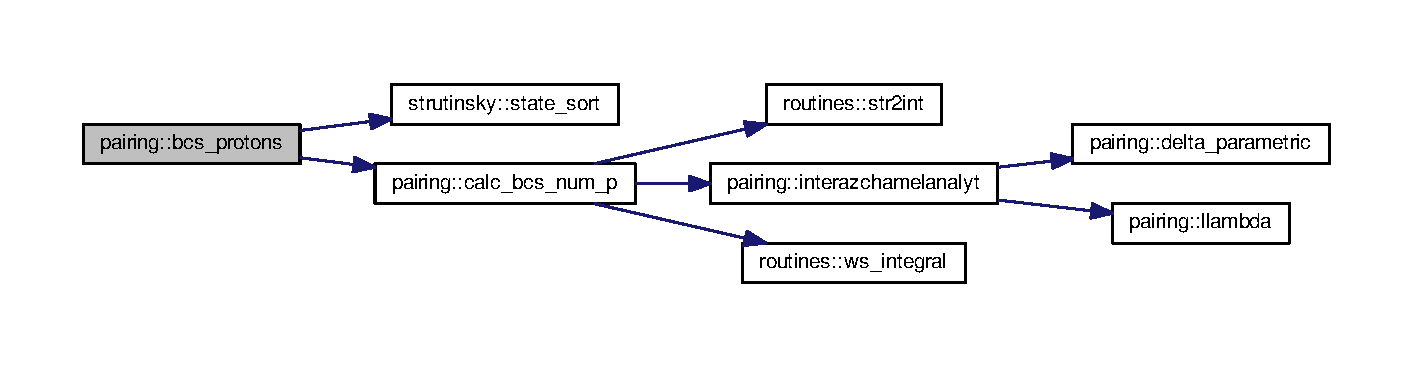
\includegraphics[width=350pt]{namespacepairing_a693cac2cfa7fcb7ad19984fefe20495c_cgraph}
\end{center}
\end{figure}
Here is the caller graph for this function\+:
\nopagebreak
\begin{figure}[H]
\begin{center}
\leavevmode
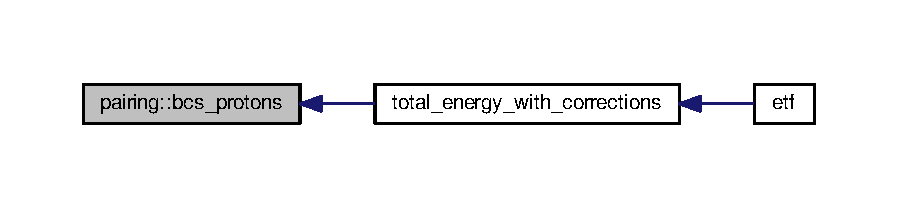
\includegraphics[width=350pt]{namespacepairing_a693cac2cfa7fcb7ad19984fefe20495c_icgraph}
\end{center}
\end{figure}
\mbox{\Hypertarget{namespacepairing_a37440fb2ff0d8a3495d051f3f14c9107}\label{namespacepairing_a37440fb2ff0d8a3495d051f3f14c9107}} 
\index{pairing@{pairing}!calc\+\_\+bcs\+\_\+num\+\_\+p@{calc\+\_\+bcs\+\_\+num\+\_\+p}}
\index{calc\+\_\+bcs\+\_\+num\+\_\+p@{calc\+\_\+bcs\+\_\+num\+\_\+p}!pairing@{pairing}}
\subsubsection{\texorpdfstring{calc\+\_\+bcs\+\_\+num\+\_\+p()}{calc\_bcs\_num\_p()}}
{\footnotesize\ttfamily real(kind=dp) function pairing\+::calc\+\_\+bcs\+\_\+num\+\_\+p (\begin{DoxyParamCaption}\item[{real(kind=dp), intent(in)}]{mu\+\_\+p }\end{DoxyParamCaption})}



Function to solve gap equation at given chemical potential \char`\"{}mu\+\_\+p\char`\"{}, returning the (B\+CS) number of protons. 

\begin{DoxyAuthor}{Author}
M. Shelley, A. Pastore 
\end{DoxyAuthor}

\begin{DoxyParams}[1]{Parameters}
\mbox{\tt in}  & {\em mu\+\_\+p} & Proton chemical potential \\
\hline
\end{DoxyParams}
Here is the call graph for this function\+:
\nopagebreak
\begin{figure}[H]
\begin{center}
\leavevmode
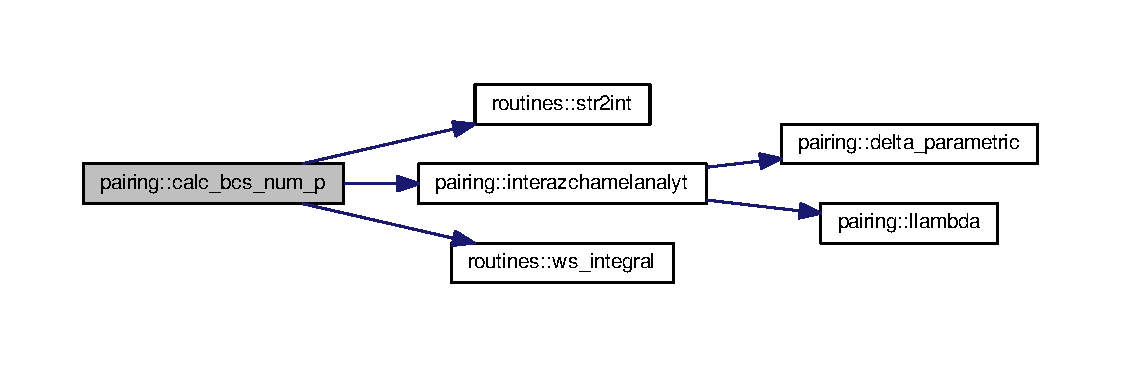
\includegraphics[width=350pt]{namespacepairing_a37440fb2ff0d8a3495d051f3f14c9107_cgraph}
\end{center}
\end{figure}
Here is the caller graph for this function\+:
\nopagebreak
\begin{figure}[H]
\begin{center}
\leavevmode
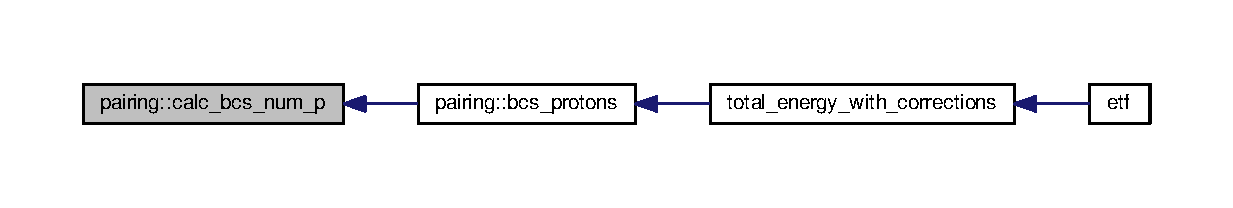
\includegraphics[width=350pt]{namespacepairing_a37440fb2ff0d8a3495d051f3f14c9107_icgraph}
\end{center}
\end{figure}
\mbox{\Hypertarget{namespacepairing_ac34989a934af1e6a63131c619426c5aa}\label{namespacepairing_ac34989a934af1e6a63131c619426c5aa}} 
\index{pairing@{pairing}!calc\+\_\+e\+\_\+pair@{calc\+\_\+e\+\_\+pair}}
\index{calc\+\_\+e\+\_\+pair@{calc\+\_\+e\+\_\+pair}!pairing@{pairing}}
\subsubsection{\texorpdfstring{calc\+\_\+e\+\_\+pair()}{calc\_e\_pair()}}
{\footnotesize\ttfamily subroutine pairing\+::calc\+\_\+e\+\_\+pair (\begin{DoxyParamCaption}{ }\end{DoxyParamCaption})}



Subroutine to calculate the pairing energy for the WS cell, using the method specified in \char`\"{}input.\+in\char`\"{}. 

\begin{DoxyAuthor}{Author}
M. Shelley 
\end{DoxyAuthor}
Here is the call graph for this function\+:
\nopagebreak
\begin{figure}[H]
\begin{center}
\leavevmode
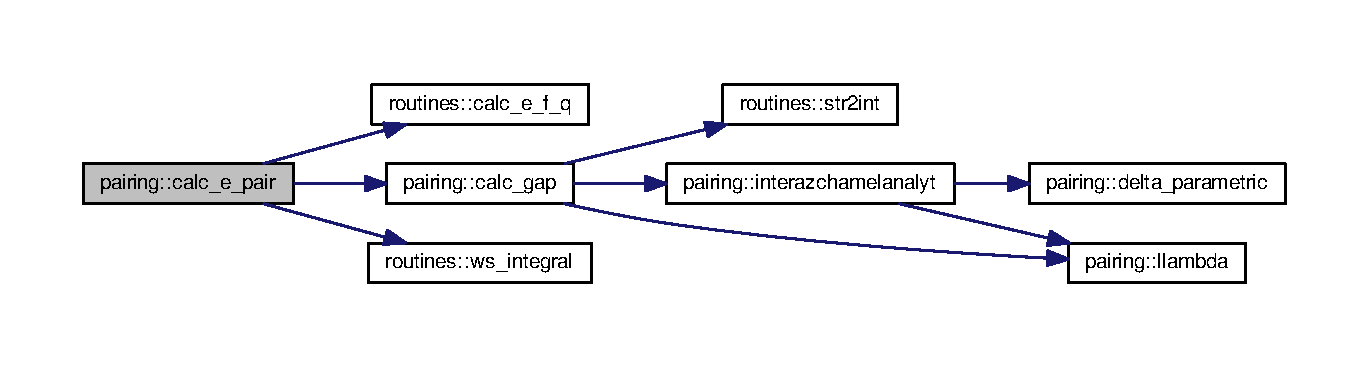
\includegraphics[width=350pt]{namespacepairing_ac34989a934af1e6a63131c619426c5aa_cgraph}
\end{center}
\end{figure}
Here is the caller graph for this function\+:
\nopagebreak
\begin{figure}[H]
\begin{center}
\leavevmode
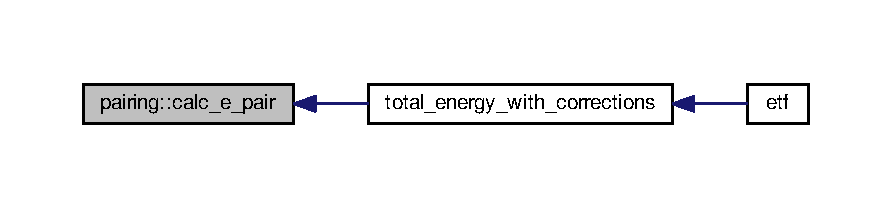
\includegraphics[width=350pt]{namespacepairing_ac34989a934af1e6a63131c619426c5aa_icgraph}
\end{center}
\end{figure}
\mbox{\Hypertarget{namespacepairing_abad69eb8cb33077add1b9da84bff7c55}\label{namespacepairing_abad69eb8cb33077add1b9da84bff7c55}} 
\index{pairing@{pairing}!calc\+\_\+gap@{calc\+\_\+gap}}
\index{calc\+\_\+gap@{calc\+\_\+gap}!pairing@{pairing}}
\subsubsection{\texorpdfstring{calc\+\_\+gap()}{calc\_gap()}}
{\footnotesize\ttfamily real(kind=dp) function pairing\+::calc\+\_\+gap (\begin{DoxyParamCaption}\item[{real(kind=dp), intent(in)}]{r,  }\item[{real(kind=dp), intent(in)}]{rhon,  }\item[{real(kind=dp), intent(in)}]{rhop,  }\item[{real(kind=dp), intent(in)}]{fq,  }\item[{real(kind=dp), intent(in)}]{mu }\end{DoxyParamCaption})}



Function to calculate the pairing gap in infinite neutron matter, for specified density and effective mass. 

\begin{DoxyAuthor}{Author}
M. Shelley 
\end{DoxyAuthor}

\begin{DoxyParams}[1]{Parameters}
\mbox{\tt in}  & {\em r} & Radius \\
\hline
\mbox{\tt in}  & {\em rhon} & Neutron density \\
\hline
\mbox{\tt in}  & {\em rhop} & Proton density \\
\hline
\mbox{\tt in}  & {\em fq} & Effective mass \\
\hline
\mbox{\tt in}  & {\em mu} & Effective chemical potential \\
\hline
\end{DoxyParams}
Here is the call graph for this function\+:
\nopagebreak
\begin{figure}[H]
\begin{center}
\leavevmode
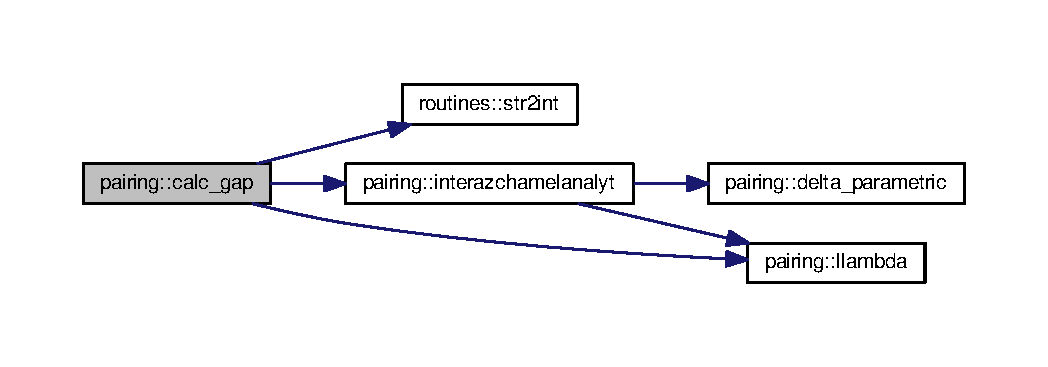
\includegraphics[width=350pt]{namespacepairing_abad69eb8cb33077add1b9da84bff7c55_cgraph}
\end{center}
\end{figure}
Here is the caller graph for this function\+:
\nopagebreak
\begin{figure}[H]
\begin{center}
\leavevmode
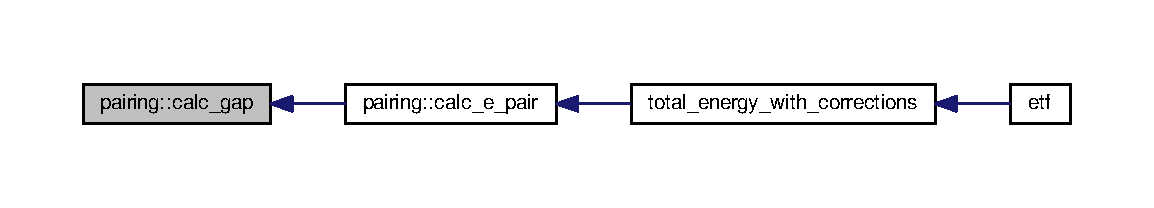
\includegraphics[width=350pt]{namespacepairing_abad69eb8cb33077add1b9da84bff7c55_icgraph}
\end{center}
\end{figure}
\mbox{\Hypertarget{namespacepairing_aaa0b619b1e454229caef01a56d0a61fd}\label{namespacepairing_aaa0b619b1e454229caef01a56d0a61fd}} 
\index{pairing@{pairing}!delta\+\_\+parametric@{delta\+\_\+parametric}}
\index{delta\+\_\+parametric@{delta\+\_\+parametric}!pairing@{pairing}}
\subsubsection{\texorpdfstring{delta\+\_\+parametric()}{delta\_parametric()}}
{\footnotesize\ttfamily real(kind=dp) function pairing\+::delta\+\_\+parametric (\begin{DoxyParamCaption}\item[{real(kind=dp), intent(in)}]{kf,  }\item[{real(kind=dp), intent(in)}]{YY,  }\item[{integer, intent(in)}]{itz,  }\item[{real(kind=dp), intent(in)}]{xk0 }\end{DoxyParamCaption})}



Function to calculate the pairing gap using the analytical B\+Sk expression. Modified by M. Shelley. 

\begin{DoxyAuthor}{Author}
A. Pastore, M. Shelley 
\end{DoxyAuthor}

\begin{DoxyParams}[1]{Parameters}
\mbox{\tt in}  & {\em kf} & Fermi momentum \\
\hline
\mbox{\tt in}  & {\em YY} & Neutron-\/proton composition \\
\hline
\mbox{\tt in}  & {\em itz} & Isospin \\
\hline
\mbox{\tt in}  & {\em xk0} & \char`\"{}\+Average\char`\"{} fermi momentum \\
\hline
\end{DoxyParams}
Here is the caller graph for this function\+:
\nopagebreak
\begin{figure}[H]
\begin{center}
\leavevmode
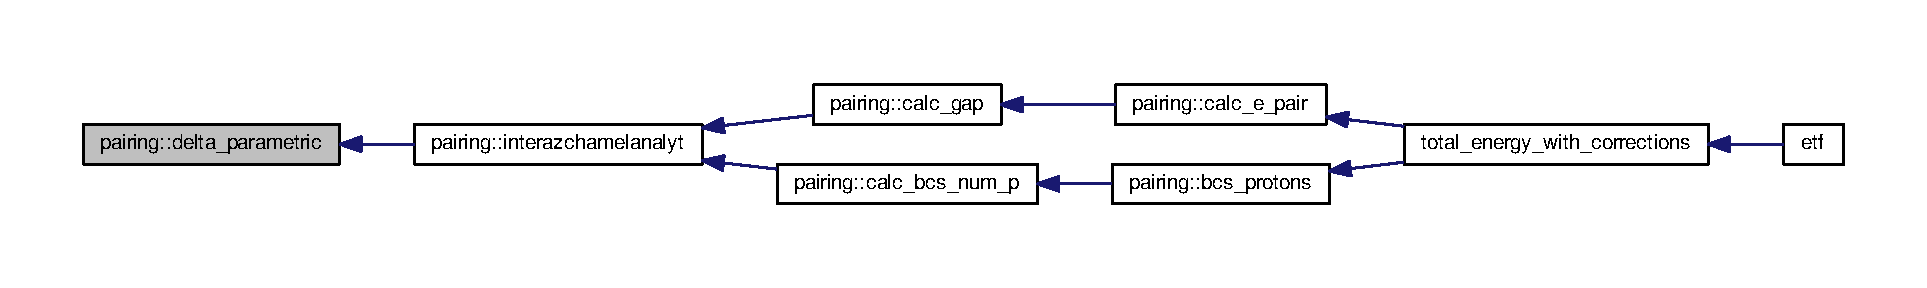
\includegraphics[width=350pt]{namespacepairing_aaa0b619b1e454229caef01a56d0a61fd_icgraph}
\end{center}
\end{figure}
\mbox{\Hypertarget{namespacepairing_aebb21947c7228a3fb9a092edfa226662}\label{namespacepairing_aebb21947c7228a3fb9a092edfa226662}} 
\index{pairing@{pairing}!interazchamelanalyt@{interazchamelanalyt}}
\index{interazchamelanalyt@{interazchamelanalyt}!pairing@{pairing}}
\subsubsection{\texorpdfstring{interazchamelanalyt()}{interazchamelanalyt()}}
{\footnotesize\ttfamily real(kind=dp) function pairing\+::interazchamelanalyt (\begin{DoxyParamCaption}\item[{real(kind=dp), intent(in)}]{rhon,  }\item[{real(kind=dp), intent(in)}]{rhop,  }\item[{real(kind=dp), intent(in)}]{hbm,  }\item[{integer, intent(in)}]{itz }\end{DoxyParamCaption})}



Function to calculate the interaction strength for the effective contact pairing force. Modified by M. Shelley. 

\begin{DoxyAuthor}{Author}
A. Pastore, M. Shelley 
\end{DoxyAuthor}

\begin{DoxyParams}[1]{Parameters}
\mbox{\tt in}  & {\em rhon} & Neutron density \\
\hline
\mbox{\tt in}  & {\em rhop} & Proton density \\
\hline
\mbox{\tt in}  & {\em hbm} & $\frac{\hbar^2}{2m^*}$ \\
\hline
\mbox{\tt in}  & {\em itz} & Isospin \\
\hline
\end{DoxyParams}
Here is the call graph for this function\+:
\nopagebreak
\begin{figure}[H]
\begin{center}
\leavevmode
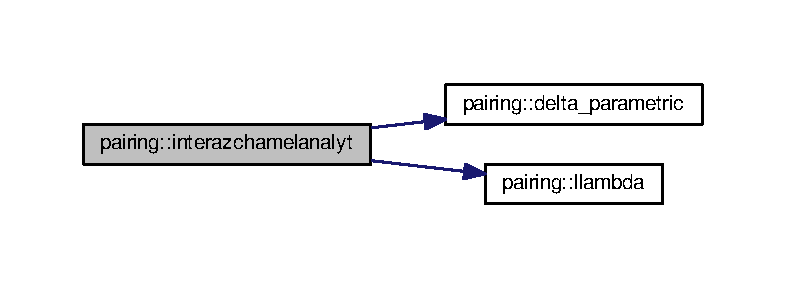
\includegraphics[width=350pt]{namespacepairing_aebb21947c7228a3fb9a092edfa226662_cgraph}
\end{center}
\end{figure}
Here is the caller graph for this function\+:
\nopagebreak
\begin{figure}[H]
\begin{center}
\leavevmode
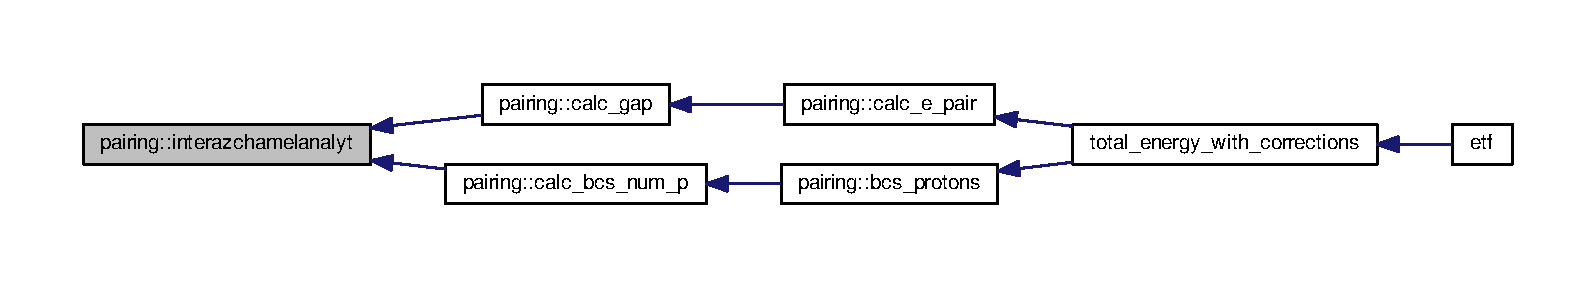
\includegraphics[width=350pt]{namespacepairing_aebb21947c7228a3fb9a092edfa226662_icgraph}
\end{center}
\end{figure}
\mbox{\Hypertarget{namespacepairing_ab022f3dcf7994e9f95315b3b2007a9ee}\label{namespacepairing_ab022f3dcf7994e9f95315b3b2007a9ee}} 
\index{pairing@{pairing}!llambda@{llambda}}
\index{llambda@{llambda}!pairing@{pairing}}
\subsubsection{\texorpdfstring{llambda()}{llambda()}}
{\footnotesize\ttfamily real(kind=dp) function pairing\+::llambda (\begin{DoxyParamCaption}\item[{real(kind=dp), intent(in)}]{x }\end{DoxyParamCaption})}



Function to calculate the pairing cutoff for the effective contact pairing force. 

\begin{DoxyAuthor}{Author}
A. Pastore 
\end{DoxyAuthor}

\begin{DoxyParams}[1]{Parameters}
\mbox{\tt in}  & {\em x} & (D\+D\+CI cutoff) / (Fermi energy) \\
\hline
\end{DoxyParams}
Here is the caller graph for this function\+:
\nopagebreak
\begin{figure}[H]
\begin{center}
\leavevmode
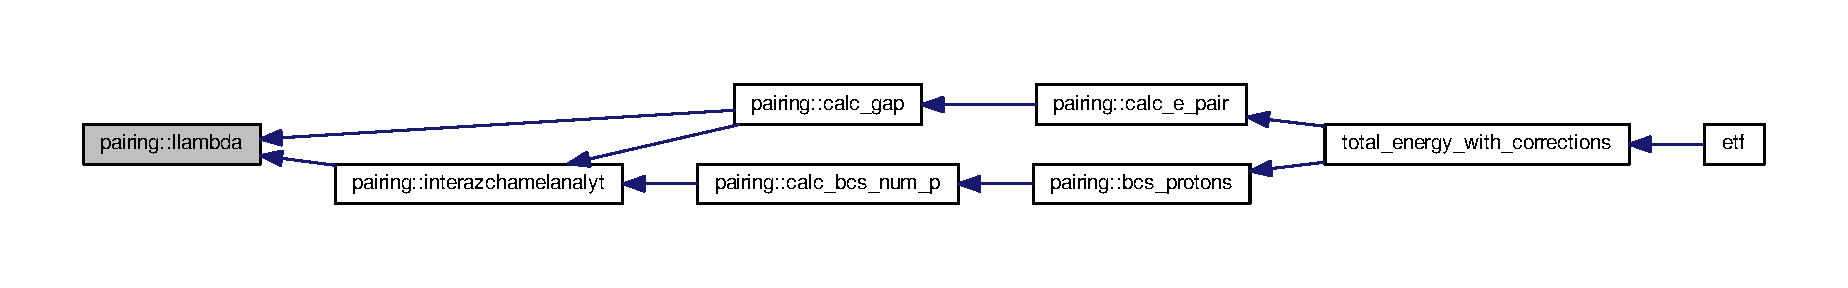
\includegraphics[width=350pt]{namespacepairing_ab022f3dcf7994e9f95315b3b2007a9ee_icgraph}
\end{center}
\end{figure}

\hypertarget{namespaceparameters}{}\section{parameters Module Reference}
\label{namespaceparameters}\index{parameters@{parameters}}


Module to hold global parameters and variables.  


\subsection*{Functions/\+Subroutines}
\begin{DoxyCompactItemize}
\item 
subroutine \mbox{\hyperlink{namespaceparameters_a55242f635842d12dbb53d66ae9248b93}{force\+\_\+initialise}} ()
\begin{DoxyCompactList}\small\item\em Subroutine to initialise Skyrme force parameters with values for a given force specified in \textquotesingle{}input.\+dat\textquotesingle{}. \end{DoxyCompactList}\end{DoxyCompactItemize}
\subsection*{Variables}
\begin{DoxyCompactItemize}
\item 
integer, parameter \mbox{\hyperlink{namespaceparameters_a52f8c6351fd79345d8811e065bcbbb37}{dp}} = selected\+\_\+real\+\_\+kind(15, 300)
\begin{DoxyCompactList}\small\item\em Precision. \end{DoxyCompactList}\item 
real(kind=\mbox{\hyperlink{namespaceparameters_a52f8c6351fd79345d8811e065bcbbb37}{dp}}), parameter \mbox{\hyperlink{group__CONSTANTS_ga399aac088b57a76a8a5a3784448ba3cf}{pi}} = 3.\+1415926535897932\+\_\+dp
\begin{DoxyCompactList}\small\item\em $\pi$ \end{DoxyCompactList}\item 
real(kind=\mbox{\hyperlink{namespaceparameters_a52f8c6351fd79345d8811e065bcbbb37}{dp}}), parameter \mbox{\hyperlink{group__CONSTANTS_gad4b06975615fad2c991376a975fd08f1}{hbar2\+\_\+2m}} = 20.\+73553\+\_\+dp
\begin{DoxyCompactList}\small\item\em $\frac{\hbar^2}{2m}$ for S\+Ly forces \end{DoxyCompactList}\item 
real(kind=\mbox{\hyperlink{namespaceparameters_a52f8c6351fd79345d8811e065bcbbb37}{dp}}), parameter \mbox{\hyperlink{group__CONSTANTS_ga0796781a51dc993c4b563f7ac404c641}{rho0}} = 0.\+16\+\_\+dp
\begin{DoxyCompactList}\small\item\em $\rho_0$, nuclear saturation density $[fm^{-3}]$ \end{DoxyCompactList}\item 
real(kind=\mbox{\hyperlink{namespaceparameters_a52f8c6351fd79345d8811e065bcbbb37}{dp}}), parameter \mbox{\hyperlink{group__CONSTANTS_gaafa6a6262bc00c89fb3d403241497d22}{e2}} = 1.\+439978408596513\+\_\+dp
\begin{DoxyCompactList}\small\item\em $e^2$, electric charge squared $[MeV\cdot fm]$ \end{DoxyCompactList}\item 
real(kind=\mbox{\hyperlink{namespaceparameters_a52f8c6351fd79345d8811e065bcbbb37}{dp}}), parameter \mbox{\hyperlink{group__CONSTANTS_ga8b91e60e1e7c4b066cc282415c740bc9}{mec2}} = 0.\+51099895\+\_\+dp
\begin{DoxyCompactList}\small\item\em Electron rest mass $[MeV/c^2]$. \end{DoxyCompactList}\item 
real(kind=\mbox{\hyperlink{namespaceparameters_a52f8c6351fd79345d8811e065bcbbb37}{dp}}), parameter \mbox{\hyperlink{group__CONSTANTS_ga3cd51d33e13930045ff98294b5044e2c}{mnc2}} = 939.\+56542052\+\_\+dp
\item 
real(kind=\mbox{\hyperlink{namespaceparameters_a52f8c6351fd79345d8811e065bcbbb37}{dp}}), parameter \mbox{\hyperlink{group__CONSTANTS_ga2e354d662a28a3a09a9819c54f818dab}{mpc2}} = 938.\+27208816\+\_\+dp
\item 
real(kind=\mbox{\hyperlink{namespaceparameters_a52f8c6351fd79345d8811e065bcbbb37}{dp}}), parameter \mbox{\hyperlink{group__CONSTANTS_gafb47622609b676d956b2c58f4b909064}{hbarc}} = 197.\+3269804\+\_\+dp
\begin{DoxyCompactList}\small\item\em $\hbar*c$ \end{DoxyCompactList}\item 
real(kind=\mbox{\hyperlink{namespaceparameters_a52f8c6351fd79345d8811e065bcbbb37}{dp}}), parameter \mbox{\hyperlink{group__HBAR2__2M_gaa00326a999bcae07e22d89387404ac19}{mamuc2}} = 931.\+49386\+\_\+dp
\begin{DoxyCompactList}\small\item\em Atomic mass unit $u$. \end{DoxyCompactList}\item 
real(kind=\mbox{\hyperlink{namespaceparameters_a52f8c6351fd79345d8811e065bcbbb37}{dp}}), parameter \mbox{\hyperlink{group__HBAR2__2M_gaad7518fe64b61c89a5fdca4244b22af1}{xmh}} = 7.\+28896940\+\_\+dp
\item 
real(kind=\mbox{\hyperlink{namespaceparameters_a52f8c6351fd79345d8811e065bcbbb37}{dp}}), parameter \mbox{\hyperlink{group__HBAR2__2M_ga1ee1de4838adf9dd601aa5c6d518709c}{rydb}} = 13.\+6056981e-\/6\+\_\+dp
\begin{DoxyCompactList}\small\item\em Rydberg constant. \end{DoxyCompactList}\item 
real(kind=\mbox{\hyperlink{namespaceparameters_a52f8c6351fd79345d8811e065bcbbb37}{dp}}), parameter \mbox{\hyperlink{group__HBAR2__2M_gaca637757baec6d59dc2b73dcf21b6b3d}{xmp}} = \mbox{\hyperlink{group__HBAR2__2M_gaad7518fe64b61c89a5fdca4244b22af1}{xmh}} -\/ \mbox{\hyperlink{group__CONSTANTS_ga8b91e60e1e7c4b066cc282415c740bc9}{mec2}} + \mbox{\hyperlink{group__HBAR2__2M_ga1ee1de4838adf9dd601aa5c6d518709c}{rydb}}
\item 
real(kind=\mbox{\hyperlink{namespaceparameters_a52f8c6351fd79345d8811e065bcbbb37}{dp}}), parameter \mbox{\hyperlink{group__HBAR2__2M_ga54928a3b468a11418226e44d5f2337ce}{xmn}} = 8.\+07132281\+\_\+dp
\item 
real(kind=\mbox{\hyperlink{namespaceparameters_a52f8c6351fd79345d8811e065bcbbb37}{dp}}), parameter \mbox{\hyperlink{group__FRACTIONS_ga22877764fb6363b2fa930793c57a03da}{fr12}} = 1.\+\_\+dp/2
\item 
real(kind=\mbox{\hyperlink{namespaceparameters_a52f8c6351fd79345d8811e065bcbbb37}{dp}}), parameter \mbox{\hyperlink{group__FRACTIONS_gaffec0a7933c65703944576ebea0c1cd1}{fr14}} = 1.\+\_\+dp/4
\item 
real(kind=\mbox{\hyperlink{namespaceparameters_a52f8c6351fd79345d8811e065bcbbb37}{dp}}), parameter \mbox{\hyperlink{group__FRACTIONS_ga59c72e10a23b892113d106b25c1f60d7}{fr18}} = 1.\+\_\+dp/8
\item 
real(kind=\mbox{\hyperlink{namespaceparameters_a52f8c6351fd79345d8811e065bcbbb37}{dp}}), parameter \mbox{\hyperlink{group__FRACTIONS_ga49bc50cd5025d08ac8f93efb9d2f2c57}{fr1\+\_\+16}} = 1.\+\_\+dp/16
\item 
real(kind=\mbox{\hyperlink{namespaceparameters_a52f8c6351fd79345d8811e065bcbbb37}{dp}}), parameter \mbox{\hyperlink{group__FRACTIONS_ga9d703cf8cb03df7ac75c98494659c894}{fr1\+\_\+32}} = 1.\+\_\+dp/32
\item 
real(kind=\mbox{\hyperlink{namespaceparameters_a52f8c6351fd79345d8811e065bcbbb37}{dp}}), parameter \mbox{\hyperlink{group__FRACTIONS_ga7012f1eaa8d54fce4923459913c9ea89}{fr13}} = 1.\+\_\+dp/3
\item 
real(kind=\mbox{\hyperlink{namespaceparameters_a52f8c6351fd79345d8811e065bcbbb37}{dp}}), parameter \mbox{\hyperlink{group__FRACTIONS_ga67d2b3b04777af92b519826b97ce69a4}{fr16}} = 1.\+\_\+dp/6
\item 
real(kind=\mbox{\hyperlink{namespaceparameters_a52f8c6351fd79345d8811e065bcbbb37}{dp}}), parameter \mbox{\hyperlink{group__FRACTIONS_gaa8dad9cec662853b1633da29ad89f6aa}{fr1\+\_\+12}} = 1.\+\_\+dp/12
\item 
real(kind=\mbox{\hyperlink{namespaceparameters_a52f8c6351fd79345d8811e065bcbbb37}{dp}}), parameter \mbox{\hyperlink{group__FRACTIONS_ga6f3d13faca548dd3fb16645525651743}{fr1\+\_\+24}} = 1.\+\_\+dp/24
\item 
real(kind=\mbox{\hyperlink{namespaceparameters_a52f8c6351fd79345d8811e065bcbbb37}{dp}}), parameter \mbox{\hyperlink{group__FRACTIONS_gaa55c45ce58d2200ffa6ff168d00e94d7}{fr1\+\_\+36}} = 1.\+\_\+dp/36
\item 
real(kind=\mbox{\hyperlink{namespaceparameters_a52f8c6351fd79345d8811e065bcbbb37}{dp}}), parameter \mbox{\hyperlink{group__FRACTIONS_gaf550152b4a78556eab5e45a3505a690e}{fr23}} = 2.\+\_\+dp/3
\item 
real(kind=\mbox{\hyperlink{namespaceparameters_a52f8c6351fd79345d8811e065bcbbb37}{dp}}), parameter \mbox{\hyperlink{group__FRACTIONS_gaae4b443a271ca66ffd82ed02a3062073}{fr29}} = 2.\+\_\+dp/9
\item 
real(kind=\mbox{\hyperlink{namespaceparameters_a52f8c6351fd79345d8811e065bcbbb37}{dp}}), parameter \mbox{\hyperlink{group__FRACTIONS_gadb06185f00fedb4688eb75250f7365de}{fr32}} = 3.\+\_\+dp/2
\item 
real(kind=\mbox{\hyperlink{namespaceparameters_a52f8c6351fd79345d8811e065bcbbb37}{dp}}), parameter \mbox{\hyperlink{group__FRACTIONS_ga8f9972a5fa3d36c2893e702ab70c7fff}{fr34}} = 3.\+\_\+dp/4
\item 
real(kind=\mbox{\hyperlink{namespaceparameters_a52f8c6351fd79345d8811e065bcbbb37}{dp}}), parameter \mbox{\hyperlink{group__FRACTIONS_ga51fd0944911031e89f45e11247545886}{fr35}} = 3.\+\_\+dp/5
\item 
real(kind=\mbox{\hyperlink{namespaceparameters_a52f8c6351fd79345d8811e065bcbbb37}{dp}}), parameter \mbox{\hyperlink{group__FRACTIONS_ga7fcdf682bf3d4c7901343542bcee3976}{fr38}} = 3.\+\_\+dp/8
\item 
real(kind=\mbox{\hyperlink{namespaceparameters_a52f8c6351fd79345d8811e065bcbbb37}{dp}}), parameter \mbox{\hyperlink{group__FRACTIONS_gadb8dc3cfa1864abcbb3226845f3d1953}{fr3\+\_\+10}} = 3.\+\_\+dp/10
\item 
real(kind=\mbox{\hyperlink{namespaceparameters_a52f8c6351fd79345d8811e065bcbbb37}{dp}}), parameter \mbox{\hyperlink{group__FRACTIONS_ga1705bf89adaf6e54bdf027386ecdc5a9}{fr43}} = 4.\+\_\+dp/3
\item 
real(kind=\mbox{\hyperlink{namespaceparameters_a52f8c6351fd79345d8811e065bcbbb37}{dp}}), parameter \mbox{\hyperlink{group__FRACTIONS_ga348f3739fc94f9786aeb6045a5c9c76b}{fr53}} = 5.\+\_\+dp/3
\item 
real(kind=\mbox{\hyperlink{namespaceparameters_a52f8c6351fd79345d8811e065bcbbb37}{dp}}), parameter \mbox{\hyperlink{group__FRACTIONS_ga4b5dee914c69f248bc576e0ef5a48cad}{fr54}} = 5.\+\_\+dp/4
\item 
real(kind=\mbox{\hyperlink{namespaceparameters_a52f8c6351fd79345d8811e065bcbbb37}{dp}}), parameter \mbox{\hyperlink{group__FRACTIONS_ga74e22f362165a8830c6acb135f54921a}{fr83}} = 8.\+\_\+dp/3
\item 
real(kind=\mbox{\hyperlink{namespaceparameters_a52f8c6351fd79345d8811e065bcbbb37}{dp}}), parameter \mbox{\hyperlink{group__FRACTIONS_ga5a9e77cd58019aeeb71cd5be86faf68f}{fr260\+\_\+3}} = 260.\+\_\+dp/3
\item 
real(kind=\mbox{\hyperlink{namespaceparameters_a52f8c6351fd79345d8811e065bcbbb37}{dp}}) \mbox{\hyperlink{group__SKYRME__PARS_gabbfefb4415d1278f79fd07d05105335a}{w0}}
\begin{DoxyCompactList}\small\item\em Spin-\/orbit strength $W_0$. \end{DoxyCompactList}\item 
real(kind=\mbox{\hyperlink{namespaceparameters_a52f8c6351fd79345d8811e065bcbbb37}{dp}}) \mbox{\hyperlink{group__SKYRME__PARS_gadbebfa135603ae9f34b4a98ac62ce8d8}{t0}}
\item 
real(kind=\mbox{\hyperlink{namespaceparameters_a52f8c6351fd79345d8811e065bcbbb37}{dp}}) \mbox{\hyperlink{group__SKYRME__PARS_ga86c5690b49e0b02be9cae32459f6cc37}{x0}}
\item 
real(kind=\mbox{\hyperlink{namespaceparameters_a52f8c6351fd79345d8811e065bcbbb37}{dp}}) \mbox{\hyperlink{group__SKYRME__PARS_ga2104f8e3f4c55a866272683975f6acd0}{t1}}
\item 
real(kind=\mbox{\hyperlink{namespaceparameters_a52f8c6351fd79345d8811e065bcbbb37}{dp}}) \mbox{\hyperlink{group__SKYRME__PARS_ga17d86815551fd59fbeaba6cc8e54438b}{x1}}
\item 
real(kind=\mbox{\hyperlink{namespaceparameters_a52f8c6351fd79345d8811e065bcbbb37}{dp}}) \mbox{\hyperlink{group__SKYRME__PARS_ga28e545481d284c866487bfb61e918159}{t2}}
\item 
real(kind=\mbox{\hyperlink{namespaceparameters_a52f8c6351fd79345d8811e065bcbbb37}{dp}}) \mbox{\hyperlink{group__SKYRME__PARS_ga505cd8d8fea1c311291e29cfb0516c91}{x2}}
\item 
real(kind=\mbox{\hyperlink{namespaceparameters_a52f8c6351fd79345d8811e065bcbbb37}{dp}}) \mbox{\hyperlink{group__SKYRME__PARS_ga41ad159facccbc41a3a4bf58942da03d}{t3}}
\item 
real(kind=\mbox{\hyperlink{namespaceparameters_a52f8c6351fd79345d8811e065bcbbb37}{dp}}) \mbox{\hyperlink{group__SKYRME__PARS_ga361bcdef664c7f70557bcc2f42b2abce}{x3}}
\item 
real(kind=\mbox{\hyperlink{namespaceparameters_a52f8c6351fd79345d8811e065bcbbb37}{dp}}) \mbox{\hyperlink{group__SKYRME__PARS_ga3726a27918a1e2929cdac9ffd451ec14}{sigma}}
\item 
real(kind=\mbox{\hyperlink{namespaceparameters_a52f8c6351fd79345d8811e065bcbbb37}{dp}}), dimension(0\+:1) \mbox{\hyperlink{group__SKYRME__PARS_ga8eaaa7306780e89ea9299163596ebc7f}{hbar2\+\_\+2m\+\_\+q}}
\begin{DoxyCompactList}\small\item\em $\frac{\hbar^2}{2m}$ with isospin dependence, as required by B\+Sk forces \end{DoxyCompactList}\item 
logical \mbox{\hyperlink{group__SKYRME__PARS_ga8d1441b6c74260a2058e73213ae60941}{j2\+\_\+terms}}
\begin{DoxyCompactList}\small\item\em Whether functional uses $\textbf{J}^2$ terms. \end{DoxyCompactList}\item 
real(kind=\mbox{\hyperlink{namespaceparameters_a52f8c6351fd79345d8811e065bcbbb37}{dp}}) \mbox{\hyperlink{group__SKYRME__COEFFS_ga370f8790e2b550acb651df944341c38a}{b1}}
\item 
real(kind=\mbox{\hyperlink{namespaceparameters_a52f8c6351fd79345d8811e065bcbbb37}{dp}}) \mbox{\hyperlink{group__SKYRME__COEFFS_gafeab3f7d25c9403fc9278f88e131e394}{b2}}
\item 
real(kind=\mbox{\hyperlink{namespaceparameters_a52f8c6351fd79345d8811e065bcbbb37}{dp}}) \mbox{\hyperlink{group__SKYRME__COEFFS_ga9b2ac7e2a2fd38fad3f2d4aa9eb74827}{b3}}
\item 
real(kind=\mbox{\hyperlink{namespaceparameters_a52f8c6351fd79345d8811e065bcbbb37}{dp}}) \mbox{\hyperlink{group__SKYRME__COEFFS_gaa0e98c8120ce5a6ee2c59e99e54b1564}{b4}}
\item 
real(kind=\mbox{\hyperlink{namespaceparameters_a52f8c6351fd79345d8811e065bcbbb37}{dp}}) \mbox{\hyperlink{group__SKYRME__COEFFS_ga86d34226c6b6f89e732f7acb9d6fc53d}{b5}}
\item 
real(kind=\mbox{\hyperlink{namespaceparameters_a52f8c6351fd79345d8811e065bcbbb37}{dp}}) \mbox{\hyperlink{group__SKYRME__COEFFS_ga375601587cabd94f376823158f6b3573}{b6}}
\item 
real(kind=\mbox{\hyperlink{namespaceparameters_a52f8c6351fd79345d8811e065bcbbb37}{dp}}) \mbox{\hyperlink{group__SKYRME__COEFFS_ga93c2fa7fcb7fac6304867a02d6fb21c3}{b7}}
\item 
real(kind=\mbox{\hyperlink{namespaceparameters_a52f8c6351fd79345d8811e065bcbbb37}{dp}}) \mbox{\hyperlink{group__SKYRME__COEFFS_ga9b6e33a75b631e3ba0f050460ffd5895}{b8}}
\item 
real(kind=\mbox{\hyperlink{namespaceparameters_a52f8c6351fd79345d8811e065bcbbb37}{dp}}) \mbox{\hyperlink{group__SKYRME__COEFFS_ga78905f183069e7fb9d101ae402ddd299}{b9}}
\item 
real(kind=\mbox{\hyperlink{namespaceparameters_a52f8c6351fd79345d8811e065bcbbb37}{dp}}) \mbox{\hyperlink{group__SKYRME__COEFFS_ga8810e38b014109a9b8eab1862dcc48d4}{b10}}
\item 
real(kind=\mbox{\hyperlink{namespaceparameters_a52f8c6351fd79345d8811e065bcbbb37}{dp}}) \mbox{\hyperlink{group__SKYRME__COEFFS_ga1590f4a1a23ab65ab7aebe0422add4d3}{b11}}
\item 
real(kind=\mbox{\hyperlink{namespaceparameters_a52f8c6351fd79345d8811e065bcbbb37}{dp}}) \mbox{\hyperlink{group__SKYRME__COEFFS_gad5af273df649cc4a1f0efdbb3a21078c}{b12}}
\item 
real(kind=\mbox{\hyperlink{namespaceparameters_a52f8c6351fd79345d8811e065bcbbb37}{dp}}) \mbox{\hyperlink{group__SKYRME__COEFFS_ga0cfa3a610d32b67d583a86f8b6e19c47}{b13}}
\item 
real(kind=\mbox{\hyperlink{namespaceparameters_a52f8c6351fd79345d8811e065bcbbb37}{dp}}) \mbox{\hyperlink{group__BSK__EXTRA__PARS_ga8490c300b1682aacdb076ab6349e11b0}{alpha}}
\item 
real(kind=\mbox{\hyperlink{namespaceparameters_a52f8c6351fd79345d8811e065bcbbb37}{dp}}) \mbox{\hyperlink{group__BSK__EXTRA__PARS_ga7c930f664bb545cbbdf20ca315bd20d8}{beta}}
\item 
real(kind=\mbox{\hyperlink{namespaceparameters_a52f8c6351fd79345d8811e065bcbbb37}{dp}}) \mbox{\hyperlink{group__BSK__EXTRA__PARS_ga1baca96d21c6817998a6c1bfadb8645b}{gamma}}
\item 
real(kind=\mbox{\hyperlink{namespaceparameters_a52f8c6351fd79345d8811e065bcbbb37}{dp}}) \mbox{\hyperlink{group__BSK__EXTRA__PARS_ga8e9070bc00ffb35cb30d29a2cdb4cb7d}{t4}}
\item 
real(kind=\mbox{\hyperlink{namespaceparameters_a52f8c6351fd79345d8811e065bcbbb37}{dp}}) \mbox{\hyperlink{group__BSK__EXTRA__PARS_ga48ff3471242a75ae841f4090057d5dda}{x4}}
\item 
real(kind=\mbox{\hyperlink{namespaceparameters_a52f8c6351fd79345d8811e065bcbbb37}{dp}}) \mbox{\hyperlink{group__BSK__EXTRA__PARS_gacca0e8bacd6526d5199e62df3e41b416}{t5}}
\item 
real(kind=\mbox{\hyperlink{namespaceparameters_a52f8c6351fd79345d8811e065bcbbb37}{dp}}) \mbox{\hyperlink{group__BSK__EXTRA__PARS_gac03740f2430e82863d9084708f78d297}{x5}}
\item 
real(kind=\mbox{\hyperlink{namespaceparameters_a52f8c6351fd79345d8811e065bcbbb37}{dp}}) \mbox{\hyperlink{group__BSK__EXTRA__PARS_ga6fd9de4a6f08fe29d2edb25db8ff5b9a}{fn\+\_\+pos}}
\item 
real(kind=\mbox{\hyperlink{namespaceparameters_a52f8c6351fd79345d8811e065bcbbb37}{dp}}) \mbox{\hyperlink{group__BSK__EXTRA__PARS_ga00dd6368c3084b28b39f9ca851465592}{fn\+\_\+neg}}
\item 
real(kind=\mbox{\hyperlink{namespaceparameters_a52f8c6351fd79345d8811e065bcbbb37}{dp}}) \mbox{\hyperlink{group__BSK__EXTRA__PARS_ga5e544dc32f83cdba34677a29c028ef40}{fp\+\_\+pos}}
\item 
real(kind=\mbox{\hyperlink{namespaceparameters_a52f8c6351fd79345d8811e065bcbbb37}{dp}}) \mbox{\hyperlink{group__BSK__EXTRA__PARS_ga6ed17804a32c9e04ddd4c244258b8610}{fp\+\_\+neg}}
\item 
real(kind=\mbox{\hyperlink{namespaceparameters_a52f8c6351fd79345d8811e065bcbbb37}{dp}}) \mbox{\hyperlink{group__BSK__EXTRA__PARS_ga383b5412e8499ce22ba113c539966123}{epsilon\+\_\+lambda}}
\item 
real(kind=\mbox{\hyperlink{namespaceparameters_a52f8c6351fd79345d8811e065bcbbb37}{dp}}), dimension(\+:), allocatable \mbox{\hyperlink{group__MESH_gab0ff28e85164200c8d56a8097bb2fe54}{r}}
\begin{DoxyCompactList}\small\item\em Mesh for r. \end{DoxyCompactList}\item 
real(kind=\mbox{\hyperlink{namespaceparameters_a52f8c6351fd79345d8811e065bcbbb37}{dp}}), dimension(\+:,\+:), allocatable \mbox{\hyperlink{group__DENSITIES_ga75b48fc89c0f01176fd8c58ced2979a8}{rho\+\_\+q}}
\item 
real(kind=\mbox{\hyperlink{namespaceparameters_a52f8c6351fd79345d8811e065bcbbb37}{dp}}), dimension(\+:,\+:), allocatable \mbox{\hyperlink{group__DENSITIES_ga8a7e7d5715287b287f2153291460783b}{del\+\_\+rho\+\_\+q}}
\item 
real(kind=\mbox{\hyperlink{namespaceparameters_a52f8c6351fd79345d8811e065bcbbb37}{dp}}), dimension(\+:,\+:), allocatable \mbox{\hyperlink{group__DENSITIES_ga9ccabc81160e04e43330cf8f61472f0e}{del2\+\_\+rho\+\_\+q}}
\item 
real(kind=\mbox{\hyperlink{namespaceparameters_a52f8c6351fd79345d8811e065bcbbb37}{dp}}), dimension(\+:), allocatable \mbox{\hyperlink{group__DENSITIES_gacd0134e8939522696ec62e629c100fd9}{rho\+\_\+t}}
\item 
real(kind=\mbox{\hyperlink{namespaceparameters_a52f8c6351fd79345d8811e065bcbbb37}{dp}}), dimension(\+:), allocatable \mbox{\hyperlink{group__DENSITIES_ga4d25fcfcb307d476b79d22bc2abe545b}{del\+\_\+rho\+\_\+t}}
\item 
real(kind=\mbox{\hyperlink{namespaceparameters_a52f8c6351fd79345d8811e065bcbbb37}{dp}}), dimension(\+:), allocatable \mbox{\hyperlink{group__DENSITIES_ga419642d914eb5865bb3537f5a4df7d34}{del2\+\_\+rho\+\_\+t}}
\item 
real(kind=\mbox{\hyperlink{namespaceparameters_a52f8c6351fd79345d8811e065bcbbb37}{dp}}), dimension(\+:,\+:), allocatable \mbox{\hyperlink{group__EFF__MASSES_ga5d14e09efe44edd96be9317868828e75}{f\+\_\+q}}
\item 
real(kind=\mbox{\hyperlink{namespaceparameters_a52f8c6351fd79345d8811e065bcbbb37}{dp}}), dimension(\+:,\+:), allocatable \mbox{\hyperlink{group__EFF__MASSES_gadd7fc7f6fdfb5f9f6303c42bfb0eb81c}{del\+\_\+f\+\_\+q}}
\item 
real(kind=\mbox{\hyperlink{namespaceparameters_a52f8c6351fd79345d8811e065bcbbb37}{dp}}), dimension(\+:,\+:), allocatable \mbox{\hyperlink{group__EFF__MASSES_ga0bdacded69f98c713231b1eeaa1a2d05}{del2\+\_\+f\+\_\+q}}
\item 
real(kind=\mbox{\hyperlink{namespaceparameters_a52f8c6351fd79345d8811e065bcbbb37}{dp}}), dimension(\+:,\+:), allocatable \mbox{\hyperlink{group__OTHER__DENSITIES_ga59950b9367b0a0afc462c00ef2eee424}{w\+\_\+q}}
\item 
real(kind=\mbox{\hyperlink{namespaceparameters_a52f8c6351fd79345d8811e065bcbbb37}{dp}}), dimension(\+:,\+:), allocatable \mbox{\hyperlink{group__OTHER__DENSITIES_ga20b386857a74ab08ec424aa7d6524f8b}{div\+\_\+w\+\_\+q}}
\item 
real(kind=\mbox{\hyperlink{namespaceparameters_a52f8c6351fd79345d8811e065bcbbb37}{dp}}), dimension(\+:,\+:), allocatable \mbox{\hyperlink{group__OTHER__DENSITIES_gae3217b84aeb9cb26575532fa2c7990cf}{u\+\_\+q}}
\item 
real(kind=\mbox{\hyperlink{namespaceparameters_a52f8c6351fd79345d8811e065bcbbb37}{dp}}), dimension(\+:,\+:), allocatable \mbox{\hyperlink{group__OTHER__DENSITIES_ga387eae15dcba990096da0b0a974f9858}{j\+\_\+2\+\_\+q}}
\item 
real(kind=\mbox{\hyperlink{namespaceparameters_a52f8c6351fd79345d8811e065bcbbb37}{dp}}), dimension(\+:,\+:), allocatable \mbox{\hyperlink{group__OTHER__DENSITIES_gad0e3f674777d52020dcc69ec065a4710}{j\+\_\+q}}
\item 
real(kind=\mbox{\hyperlink{namespaceparameters_a52f8c6351fd79345d8811e065bcbbb37}{dp}}), dimension(\+:,\+:), allocatable \mbox{\hyperlink{group__OTHER__DENSITIES_gaa93ef4a0286129df654277cffb40933b}{del\+\_\+j\+\_\+q}}
\item 
real(kind=\mbox{\hyperlink{namespaceparameters_a52f8c6351fd79345d8811e065bcbbb37}{dp}}), dimension(\+:,\+:), allocatable \mbox{\hyperlink{group__OTHER__DENSITIES_ga42f7b6eda54c2f6b7dbfbc5a0d3a1bf4}{div\+\_\+j\+\_\+2\+\_\+q}}
\item 
real(kind=\mbox{\hyperlink{namespaceparameters_a52f8c6351fd79345d8811e065bcbbb37}{dp}}), dimension(\+:,\+:), allocatable \mbox{\hyperlink{group__OTHER__DENSITIES_ga8181dfebaf3cbf23118c8322b1eed86d}{div\+\_\+j\+\_\+q}}
\item 
real(kind=\mbox{\hyperlink{namespaceparameters_a52f8c6351fd79345d8811e065bcbbb37}{dp}}), dimension(\+:,\+:), allocatable \mbox{\hyperlink{group__OTHER__DENSITIES_gab6c3712299b2394aa1cdc011d9373ab8}{tau\+\_\+tf\+\_\+q}}
\item 
real(kind=\mbox{\hyperlink{namespaceparameters_a52f8c6351fd79345d8811e065bcbbb37}{dp}}), dimension(\+:,\+:), allocatable \mbox{\hyperlink{group__OTHER__DENSITIES_ga045973682837700d382d75a8f6de7d9c}{tau\+\_\+2\+\_\+l\+\_\+q}}
\item 
real(kind=\mbox{\hyperlink{namespaceparameters_a52f8c6351fd79345d8811e065bcbbb37}{dp}}), dimension(\+:,\+:), allocatable \mbox{\hyperlink{group__OTHER__DENSITIES_ga64b5af532da52ba869f0fba447812146}{tau\+\_\+2\+\_\+nl\+\_\+q}}
\item 
real(kind=\mbox{\hyperlink{namespaceparameters_a52f8c6351fd79345d8811e065bcbbb37}{dp}}), dimension(\+:,\+:), allocatable \mbox{\hyperlink{group__OTHER__DENSITIES_ga8fa22b66605b27eaece8dbd54577ebc8}{tau\+\_\+etf\+\_\+q}}
\item 
real(kind=\mbox{\hyperlink{namespaceparameters_a52f8c6351fd79345d8811e065bcbbb37}{dp}}), dimension(\+:), allocatable \mbox{\hyperlink{group__OTHER__DENSITIES_ga403b0aed00d1b8df4af16d47bc09977f}{j\+\_\+t}}
\item 
real(kind=\mbox{\hyperlink{namespaceparameters_a52f8c6351fd79345d8811e065bcbbb37}{dp}}), dimension(\+:), allocatable \mbox{\hyperlink{group__OTHER__DENSITIES_ga1c75e349365b3d0cd01f2f1ed6fc3a06}{del\+\_\+j\+\_\+t}}
\item 
real(kind=\mbox{\hyperlink{namespaceparameters_a52f8c6351fd79345d8811e065bcbbb37}{dp}}), dimension(\+:), allocatable \mbox{\hyperlink{group__OTHER__DENSITIES_gaae73460a531438ad3711b017dc727066}{div\+\_\+j\+\_\+t}}
\item 
real(kind=\mbox{\hyperlink{namespaceparameters_a52f8c6351fd79345d8811e065bcbbb37}{dp}}), dimension(\+:), allocatable \mbox{\hyperlink{group__OTHER__DENSITIES_ga38f8f27b19a3324faae16c6831f551db}{tau\+\_\+etf\+\_\+t}}
\item 
real(kind=\mbox{\hyperlink{namespaceparameters_a52f8c6351fd79345d8811e065bcbbb37}{dp}}), dimension(\+:), allocatable \mbox{\hyperlink{group__OTHER__DENSITIES_gadb82cb07fdaadb4c3d4fc703ec7d0f32}{e\+\_\+density\+\_\+field}}
\item 
real(kind=\mbox{\hyperlink{namespaceparameters_a52f8c6351fd79345d8811e065bcbbb37}{dp}}), dimension(\+:), allocatable \mbox{\hyperlink{group__OTHER__DENSITIES_ga899215cff7de8d505ca9437a2c7a9e5d}{e\+\_\+density\+\_\+sky}}
\item 
real(kind=\mbox{\hyperlink{namespaceparameters_a52f8c6351fd79345d8811e065bcbbb37}{dp}}), dimension(\+:), allocatable \mbox{\hyperlink{group__OTHER__DENSITIES_ga7503ebd6515d35346e8989c0ace67040}{v\+\_\+c\+\_\+di}}
\item 
real(kind=\mbox{\hyperlink{namespaceparameters_a52f8c6351fd79345d8811e065bcbbb37}{dp}}), dimension(\+:), allocatable \mbox{\hyperlink{group__OTHER__DENSITIES_ga9fa9512dcae76285fafca5bf94f6d548}{v\+\_\+c\+\_\+ex}}
\item 
real(kind=\mbox{\hyperlink{namespaceparameters_a52f8c6351fd79345d8811e065bcbbb37}{dp}}), dimension(\+:), allocatable \mbox{\hyperlink{group__OTHER__DENSITIES_ga87dbb79a5a923879327d170ac2dd0554}{e\+\_\+density\+\_\+c\+\_\+di}}
\item 
real(kind=\mbox{\hyperlink{namespaceparameters_a52f8c6351fd79345d8811e065bcbbb37}{dp}}), dimension(\+:), allocatable \mbox{\hyperlink{group__OTHER__DENSITIES_gae0cdcff4839ee5f5e753521c6110a58c}{e\+\_\+density\+\_\+c\+\_\+ex}}
\item 
real(kind=\mbox{\hyperlink{namespaceparameters_a52f8c6351fd79345d8811e065bcbbb37}{dp}}), dimension(\+:), allocatable \mbox{\hyperlink{group__OTHER__DENSITIES_ga2ace64338ba159caa9b44094efffa81d}{v\+\_\+c\+\_\+pe}}
\item 
real(kind=\mbox{\hyperlink{namespaceparameters_a52f8c6351fd79345d8811e065bcbbb37}{dp}}), dimension(\+:,\+:,\+:), allocatable \mbox{\hyperlink{group__OTHER__DENSITIES_gae767b94dc83914662f299fc87eeaf623}{tau\+\_\+2\+\_\+cont\+\_\+q}}
\item 
real(kind=\mbox{\hyperlink{namespaceparameters_a52f8c6351fd79345d8811e065bcbbb37}{dp}}), dimension(\+:), allocatable \mbox{\hyperlink{group__OTHER__DENSITIES_ga06ab0886762c00b75dd1adf55f9e61a0}{rho\+\_\+ch}}
\begin{DoxyCompactList}\small\item\em Charge density. \end{DoxyCompactList}\item 
real(kind=\mbox{\hyperlink{namespaceparameters_a52f8c6351fd79345d8811e065bcbbb37}{dp}}), dimension(\+:,\+:), allocatable \mbox{\hyperlink{namespaceparameters_a0234a871e1ff1d0be38099df82c5e698}{d2\+\_\+rho\+\_\+q}}
\item 
real(kind=\mbox{\hyperlink{namespaceparameters_a52f8c6351fd79345d8811e065bcbbb37}{dp}}), dimension(\+:,\+:), allocatable \mbox{\hyperlink{namespaceparameters_a1621c80d10f0cca4fec0e20ffbdda0f5}{d3\+\_\+rho\+\_\+q}}
\item 
real(kind=\mbox{\hyperlink{namespaceparameters_a52f8c6351fd79345d8811e065bcbbb37}{dp}}), dimension(\+:,\+:), allocatable \mbox{\hyperlink{namespaceparameters_a59deaa51eaa68f574d57f364fff6c77a}{d4\+\_\+rho\+\_\+q}}
\item 
real(kind=\mbox{\hyperlink{namespaceparameters_a52f8c6351fd79345d8811e065bcbbb37}{dp}}), dimension(\+:,\+:), allocatable \mbox{\hyperlink{namespaceparameters_a4e57ed84b90c4ca5998a9cdaa8ccb2da}{d2\+\_\+f\+\_\+q}}
\item 
real(kind=\mbox{\hyperlink{namespaceparameters_a52f8c6351fd79345d8811e065bcbbb37}{dp}}), dimension(\+:,\+:), allocatable \mbox{\hyperlink{namespaceparameters_ada2cda17d0e9bccb3581a5b22a05f876}{d3\+\_\+f\+\_\+q}}
\item 
real(kind=\mbox{\hyperlink{namespaceparameters_a52f8c6351fd79345d8811e065bcbbb37}{dp}}), dimension(\+:,\+:), allocatable \mbox{\hyperlink{namespaceparameters_af226839e94cc06ff5d33f92af38a014c}{d4\+\_\+f\+\_\+q}}
\item 
real(kind=\mbox{\hyperlink{namespaceparameters_a52f8c6351fd79345d8811e065bcbbb37}{dp}}), dimension(\+:,\+:), allocatable \mbox{\hyperlink{namespaceparameters_a537af93b5aaa713688d624f145ebde80}{a\+\_\+q}}
\item 
real(kind=\mbox{\hyperlink{namespaceparameters_a52f8c6351fd79345d8811e065bcbbb37}{dp}}), dimension(\+:,\+:), allocatable \mbox{\hyperlink{namespaceparameters_aaeb8117f8c15d7a7414e15929e12b0a8}{d1\+\_\+a\+\_\+q}}
\item 
real(kind=\mbox{\hyperlink{namespaceparameters_a52f8c6351fd79345d8811e065bcbbb37}{dp}}), dimension(\+:,\+:), allocatable \mbox{\hyperlink{namespaceparameters_ab2833e12dbfca51501df8955b00dd7d0}{d2\+\_\+a\+\_\+q}}
\item 
real(kind=\mbox{\hyperlink{namespaceparameters_a52f8c6351fd79345d8811e065bcbbb37}{dp}}), dimension(\+:,\+:), allocatable \mbox{\hyperlink{namespaceparameters_a1449283e577e2769bd8bb5d57dbf1876}{d3\+\_\+a\+\_\+q}}
\item 
real(kind=\mbox{\hyperlink{namespaceparameters_a52f8c6351fd79345d8811e065bcbbb37}{dp}}), dimension(\+:,\+:), allocatable \mbox{\hyperlink{namespaceparameters_a68e56fd9914d22072aed5a180c5a17b2}{d4\+\_\+a\+\_\+q}}
\item 
real(kind=\mbox{\hyperlink{namespaceparameters_a52f8c6351fd79345d8811e065bcbbb37}{dp}}), dimension(\+:,\+:), allocatable \mbox{\hyperlink{namespaceparameters_a6722d1e0c27f2796d4e43405bd9c9d81}{tau\+\_\+4\+\_\+no\+\_\+spin\+\_\+q}}
\item 
real(kind=\mbox{\hyperlink{namespaceparameters_a52f8c6351fd79345d8811e065bcbbb37}{dp}}), dimension(\+:,\+:), allocatable \mbox{\hyperlink{namespaceparameters_a6f95c2f318204d32f47cefa370021fe4}{tau\+\_\+4\+\_\+so\+\_\+q}}
\item 
real(kind=\mbox{\hyperlink{namespaceparameters_a52f8c6351fd79345d8811e065bcbbb37}{dp}}), dimension(\+:,\+:), allocatable \mbox{\hyperlink{namespaceparameters_a41689cc1fc405b2fd02236c39ee5528c}{j\+\_\+4\+\_\+q}}
\item 
real(kind=\mbox{\hyperlink{namespaceparameters_a52f8c6351fd79345d8811e065bcbbb37}{dp}}), dimension(\+:,\+:), allocatable \mbox{\hyperlink{namespaceparameters_ab8757a22096c3d5f05f0bf953b59dff4}{div\+\_\+j\+\_\+4\+\_\+q}}
\item 
real(kind=\mbox{\hyperlink{namespaceparameters_a52f8c6351fd79345d8811e065bcbbb37}{dp}}), dimension(\+:,\+:,\+:), allocatable \mbox{\hyperlink{namespaceparameters_a1dd9d0c60fab7b85157b61471151ed92}{tau\+\_\+4\+\_\+cont\+\_\+q}}
\item 
real(kind=\mbox{\hyperlink{namespaceparameters_a52f8c6351fd79345d8811e065bcbbb37}{dp}}), dimension(0\+:1) \mbox{\hyperlink{group__WS__PROPERTIES_gace169ff7d198e04f282498a2b0ee2bc1}{n\+\_\+q}}
\begin{DoxyCompactList}\small\item\em Number of neutrons and protons. \end{DoxyCompactList}\item 
real(kind=\mbox{\hyperlink{namespaceparameters_a52f8c6351fd79345d8811e065bcbbb37}{dp}}) \mbox{\hyperlink{group__WS__PROPERTIES_ga4ea79549c467085cd4c8b95a09ac205e}{n\+\_\+t}}
\begin{DoxyCompactList}\small\item\em Total number of particles. \end{DoxyCompactList}\item 
real(kind=\mbox{\hyperlink{namespaceparameters_a52f8c6351fd79345d8811e065bcbbb37}{dp}}) \mbox{\hyperlink{group__WS__PROPERTIES_gaba6452c229b473b375ee695573482098}{e\+\_\+field}}
\begin{DoxyCompactList}\small\item\em Field energy. \end{DoxyCompactList}\item 
real(kind=\mbox{\hyperlink{namespaceparameters_a52f8c6351fd79345d8811e065bcbbb37}{dp}}) \mbox{\hyperlink{group__WS__PROPERTIES_ga5683bdc3d77765f0e39d27c0a8c07e12}{e\+\_\+skyrme}}
\begin{DoxyCompactList}\small\item\em Skyrme energy. \end{DoxyCompactList}\item 
real(kind=\mbox{\hyperlink{namespaceparameters_a52f8c6351fd79345d8811e065bcbbb37}{dp}}), dimension(0\+:1) \mbox{\hyperlink{group__WS__PROPERTIES_ga488ae2b962fd84ebc096feb2d9b86bdb}{e\+\_\+kinetic\+\_\+q}}
\begin{DoxyCompactList}\small\item\em Kinetic energy for neutron and protons. \end{DoxyCompactList}\item 
real(kind=\mbox{\hyperlink{namespaceparameters_a52f8c6351fd79345d8811e065bcbbb37}{dp}}) \mbox{\hyperlink{group__WS__PROPERTIES_ga6a028c7097c7f19416111f67d7751e0a}{e\+\_\+kinetic\+\_\+t}}
\begin{DoxyCompactList}\small\item\em Total kinetic energy. \end{DoxyCompactList}\item 
real(kind=\mbox{\hyperlink{namespaceparameters_a52f8c6351fd79345d8811e065bcbbb37}{dp}}) \mbox{\hyperlink{group__WS__PROPERTIES_ga1be7ac7adf47738e0cf4ada759e3b038}{e\+\_\+so}}
\begin{DoxyCompactList}\small\item\em Spin-\/orbit energy. \end{DoxyCompactList}\item 
real(kind=\mbox{\hyperlink{namespaceparameters_a52f8c6351fd79345d8811e065bcbbb37}{dp}}) \mbox{\hyperlink{group__WS__PROPERTIES_gad3cbae007568a7ca3045ba174fda13e0}{e\+\_\+coulomb\+\_\+di}}
\begin{DoxyCompactList}\small\item\em Direct Coulomb energy. \end{DoxyCompactList}\item 
real(kind=\mbox{\hyperlink{namespaceparameters_a52f8c6351fd79345d8811e065bcbbb37}{dp}}) \mbox{\hyperlink{group__WS__PROPERTIES_ga089d9dd6556d4555570eed570f9f71f3}{e\+\_\+coulomb\+\_\+ex}}
\begin{DoxyCompactList}\small\item\em Exhange Coulomb energy. \end{DoxyCompactList}\item 
real(kind=\mbox{\hyperlink{namespaceparameters_a52f8c6351fd79345d8811e065bcbbb37}{dp}}) \mbox{\hyperlink{group__WS__PROPERTIES_gaa693f79a53c67f65948484a0d2704154}{e\+\_\+coulomb}}
\begin{DoxyCompactList}\small\item\em Total Coulomb energy. \end{DoxyCompactList}\item 
real(kind=\mbox{\hyperlink{namespaceparameters_a52f8c6351fd79345d8811e065bcbbb37}{dp}}) \mbox{\hyperlink{group__WS__PROPERTIES_ga041ce78d1803675af0825ead4e0a512e}{e\+\_\+total}}
\begin{DoxyCompactList}\small\item\em Total energy. \end{DoxyCompactList}\item 
real(kind=\mbox{\hyperlink{namespaceparameters_a52f8c6351fd79345d8811e065bcbbb37}{dp}}), dimension(0\+:1) \mbox{\hyperlink{group__WS__PROPERTIES_ga640fd108640984ca51ba2f7cc29f2a8f}{mu\+\_\+q}}
\begin{DoxyCompactList}\small\item\em Neutron and proton chemical potential. \end{DoxyCompactList}\item 
real(kind=\mbox{\hyperlink{namespaceparameters_a52f8c6351fd79345d8811e065bcbbb37}{dp}}) \mbox{\hyperlink{group__WS__PROPERTIES_gacc0c124d82adcdfb692fb32f9e736bca}{mu\+\_\+e}}
\begin{DoxyCompactList}\small\item\em Electron chemical potential. \end{DoxyCompactList}\item 
real(kind=\mbox{\hyperlink{namespaceparameters_a52f8c6351fd79345d8811e065bcbbb37}{dp}}) \mbox{\hyperlink{group__WS__PROPERTIES_ga3025178429abf0548bda508408facd69}{mu\+\_\+c}}
\begin{DoxyCompactList}\small\item\em Coulomb interaction contribution to electron chemical potential. \end{DoxyCompactList}\item 
real(kind=\mbox{\hyperlink{namespaceparameters_a52f8c6351fd79345d8811e065bcbbb37}{dp}}) \mbox{\hyperlink{group__WS__PROPERTIES_ga44464a0deab6ab30fe9c2301379ceb71}{delta\+\_\+mu}}
\begin{DoxyCompactList}\small\item\em Overall chemical potential (beta-\/equilibrium condition) \end{DoxyCompactList}\item 
real(kind=\mbox{\hyperlink{namespaceparameters_a52f8c6351fd79345d8811e065bcbbb37}{dp}}) \mbox{\hyperlink{group__WS__PROPERTIES_ga769d654b2408c30dca03771d09945c2a}{pressure\+\_\+nucl}}
\begin{DoxyCompactList}\small\item\em Nuclear pressure. \end{DoxyCompactList}\item 
real(kind=\mbox{\hyperlink{namespaceparameters_a52f8c6351fd79345d8811e065bcbbb37}{dp}}) \mbox{\hyperlink{group__WS__PROPERTIES_ga72c16e4c25186b788d7d47eb8c87c3a4}{pressure\+\_\+e}}
\begin{DoxyCompactList}\small\item\em Electron pressure. \end{DoxyCompactList}\item 
real(kind=\mbox{\hyperlink{namespaceparameters_a52f8c6351fd79345d8811e065bcbbb37}{dp}}) \mbox{\hyperlink{group__WS__PROPERTIES_gab531cc7fbabd91f11cc2be7385cb5854}{pressure\+\_\+ex}}
\begin{DoxyCompactList}\small\item\em Coulomb exchange pressure. \end{DoxyCompactList}\item 
real(kind=\mbox{\hyperlink{namespaceparameters_a52f8c6351fd79345d8811e065bcbbb37}{dp}}) \mbox{\hyperlink{group__WS__PROPERTIES_gaf485019c788a68c4915fca156d59baa1}{pressure\+\_\+t}}
\begin{DoxyCompactList}\small\item\em Total pressure. \end{DoxyCompactList}\item 
integer \mbox{\hyperlink{group__INPUT__PARS_ga2b7774a07afe51f9f1e547e3104833e4}{run\+\_\+mode}}
\begin{DoxyCompactList}\small\item\em Mode to run code in (normal, test) \end{DoxyCompactList}\item 
logical \mbox{\hyperlink{group__INPUT__PARS_ga552f372a0ff4dff467424c48bedd6b49}{verbose}}
\begin{DoxyCompactList}\small\item\em Whether to print all extra messages about run. \end{DoxyCompactList}\item 
real(kind=\mbox{\hyperlink{namespaceparameters_a52f8c6351fd79345d8811e065bcbbb37}{dp}}) \mbox{\hyperlink{group__INPUT__PARS_gaa5f574e72af23ebd482368e0a7232ea1}{dr}}
\begin{DoxyCompactList}\small\item\em Mesh spacing of r $(fm)$. \end{DoxyCompactList}\item 
logical \mbox{\hyperlink{group__INPUT__PARS_ga4f6d2343db9c28bfad5b376839f279d7}{profile\+\_\+r\+\_\+max}}
\begin{DoxyCompactList}\small\item\em Whether to take \char`\"{}r\+\_\+max\char`\"{} from \char`\"{}r\+\_\+ws\char`\"{}. \end{DoxyCompactList}\item 
real(kind=\mbox{\hyperlink{namespaceparameters_a52f8c6351fd79345d8811e065bcbbb37}{dp}}) \mbox{\hyperlink{group__INPUT__PARS_ga9372571e59a93c139d629423a9104d69}{r\+\_\+max}}
\begin{DoxyCompactList}\small\item\em Max value of r $(fm)$. \end{DoxyCompactList}\item 
logical \mbox{\hyperlink{group__INPUT__PARS_ga65180c8e25c7c66a7ef57b72282eaecf}{specify\+\_\+n}}
\begin{DoxyCompactList}\small\item\em Whether to specify \char`\"{}n\char`\"{} instead of \char`\"{}dr\char`\"{}. \end{DoxyCompactList}\item 
integer \mbox{\hyperlink{group__INPUT__PARS_ga2e69dbce49f3e83688fe80de2ce83724}{n}}
\begin{DoxyCompactList}\small\item\em Number of mesh points. \end{DoxyCompactList}\item 
integer \mbox{\hyperlink{group__INPUT__PARS_ga4f15a67f3875d8c184795f8d71ac08aa}{force}}
\begin{DoxyCompactList}\small\item\em Force to use. \end{DoxyCompactList}\item 
integer \mbox{\hyperlink{group__INPUT__PARS_ga47ccf97217bda004b76720993db73258}{etf\+\_\+order}}
\begin{DoxyCompactList}\small\item\em Order at which to calculate kinetic energy densities. \end{DoxyCompactList}\item 
logical \mbox{\hyperlink{group__INPUT__PARS_gadebedfbc56e0abdbb5f8152a34ec9654}{coulomb\+\_\+on}}
\begin{DoxyCompactList}\small\item\em Use Coulomb interaction or not. \end{DoxyCompactList}\item 
logical \mbox{\hyperlink{group__INPUT__PARS_gac0158c8c810d8b150e942815ae3a4478}{electrons\+\_\+on}}
\begin{DoxyCompactList}\small\item\em Add electrons. \end{DoxyCompactList}\item 
integer \mbox{\hyperlink{group__INPUT__PARS_gaa0c2ce3053c1f294c8fe21270389511f}{nmaxstate}}
\begin{DoxyCompactList}\small\item\em Number of states that can be stored. \end{DoxyCompactList}\item 
integer \mbox{\hyperlink{group__INPUT__PARS_gaee5c7e64e0f524d969ac1848094fdbac}{lmax}}
\begin{DoxyCompactList}\small\item\em Maximum angular momentum of states to find. \end{DoxyCompactList}\item 
logical \mbox{\hyperlink{group__INPUT__PARS_ga6e579a9756d3f1c4d2ddc58a161b1f1a}{calc\+\_\+chem\+\_\+pots}}
\begin{DoxyCompactList}\small\item\em Calculate chemical potentials. \end{DoxyCompactList}\item 
logical, dimension(0\+:1) \mbox{\hyperlink{group__INPUT__PARS_gaad3b88a661482173813a2f76cba73b11}{strutinsky\+\_\+on}}
\begin{DoxyCompactList}\small\item\em Use Strutinsky Integral (SI) correction for neutrons and protons. \end{DoxyCompactList}\item 
real(kind=\mbox{\hyperlink{namespaceparameters_a52f8c6351fd79345d8811e065bcbbb37}{dp}}) \mbox{\hyperlink{group__INPUT__PARS_ga0dd8e62aa4b777681ce98d7c88cafdf8}{strut\+\_\+r\+\_\+max}}
\begin{DoxyCompactList}\small\item\em Max value of r to use for box for single particle states $(fm)$. \end{DoxyCompactList}\item 
logical \mbox{\hyperlink{group__INPUT__PARS_gacfc9efb68b340c8246340105af8678e0}{emax0\+\_\+mod}}
\begin{DoxyCompactList}\small\item\em Whether to modify \char`\"{}emax0\char`\"{} to always = 0. \end{DoxyCompactList}\item 
integer \mbox{\hyperlink{group__INPUT__PARS_gad6072a097df429aca7d4c3daf808ceda}{neutron\+\_\+pairing}}
\begin{DoxyCompactList}\small\item\em Type of pairing calculation to perform for neutrons. \end{DoxyCompactList}\item 
logical \mbox{\hyperlink{group__INPUT__PARS_ga7478728bc2b5fc83dee2f2c21724420c}{proton\+\_\+bcs}}
\begin{DoxyCompactList}\small\item\em Whether to do B\+CS for protons. \end{DoxyCompactList}\item 
real(kind=\mbox{\hyperlink{namespaceparameters_a52f8c6351fd79345d8811e065bcbbb37}{dp}}) \mbox{\hyperlink{group__INPUT__PARS_gaddd04025cfa9a151f25211259364f404}{pair\+\_\+qp\+\_\+cut}}
\begin{DoxyCompactList}\small\item\em Cut-\/off for quasiparticle energy for solving gap equation. \end{DoxyCompactList}\item 
logical \mbox{\hyperlink{group__INPUT__PARS_ga20f7226ffbb05232c930c81d83afee32}{smooth\+\_\+qp\+\_\+cut}}
\begin{DoxyCompactList}\small\item\em Whether to use smooth cut-\/off on quasiparticle energy. \end{DoxyCompactList}\item 
real(kind=\mbox{\hyperlink{namespaceparameters_a52f8c6351fd79345d8811e065bcbbb37}{dp}}) \mbox{\hyperlink{group__INPUT__PARS_ga0d7d7715270e262c6f4e02633947b548}{pair\+\_\+k\+\_\+max}}
\begin{DoxyCompactList}\small\item\em Maximum momentum for integral in gap equation. \end{DoxyCompactList}\item 
real(kind=\mbox{\hyperlink{namespaceparameters_a52f8c6351fd79345d8811e065bcbbb37}{dp}}) \mbox{\hyperlink{group__INPUT__PARS_gaecd0609846081f6a90f49cc0f162c9cd}{pair\+\_\+v0}}
\begin{DoxyCompactList}\small\item\em Interaction strength parameter. \end{DoxyCompactList}\item 
real(kind=\mbox{\hyperlink{namespaceparameters_a52f8c6351fd79345d8811e065bcbbb37}{dp}}) \mbox{\hyperlink{group__INPUT__PARS_gacd8c346f8b069e0dca502d57557b21e7}{pair\+\_\+eta}}
\begin{DoxyCompactList}\small\item\em Interaction parameter eta. \end{DoxyCompactList}\item 
real(kind=\mbox{\hyperlink{namespaceparameters_a52f8c6351fd79345d8811e065bcbbb37}{dp}}) \mbox{\hyperlink{group__INPUT__PARS_gaa3116e010e1f1435881ad489d7ea5dad}{pair\+\_\+alpha}}
\begin{DoxyCompactList}\small\item\em Interaction parameter alpha. \end{DoxyCompactList}\item 
real(kind=\mbox{\hyperlink{namespaceparameters_a52f8c6351fd79345d8811e065bcbbb37}{dp}}) \mbox{\hyperlink{group__INPUT__PARS_ga9b9d6d0cf64fa6e7f9dd00f5b15848bd}{pair\+\_\+tol}}
\begin{DoxyCompactList}\small\item\em Gap equation self-\/consistency tolerance. \end{DoxyCompactList}\item 
real(kind=\mbox{\hyperlink{namespaceparameters_a52f8c6351fd79345d8811e065bcbbb37}{dp}}) \mbox{\hyperlink{group__INPUT__PARS_ga6fdafa171f65aa7236a9c76ebaab4d08}{pair\+\_\+mix}}
\begin{DoxyCompactList}\small\item\em Mix of previous iteration in gap equation self-\/consistency loop. \end{DoxyCompactList}\item 
real(kind=\mbox{\hyperlink{namespaceparameters_a52f8c6351fd79345d8811e065bcbbb37}{dp}}) \mbox{\hyperlink{group__INPUT__PARS_ga1c083bc7a4e3979327020ec3e1509220}{pair\+\_\+dk}}
\begin{DoxyCompactList}\small\item\em Step size in integral in gap equation. \end{DoxyCompactList}\item 
real(kind=\mbox{\hyperlink{namespaceparameters_a52f8c6351fd79345d8811e065bcbbb37}{dp}}) \mbox{\hyperlink{group__INPUT__PARS_ga9fe26afec63d3ebfb7900ccc330779d0}{pair\+\_\+del\+\_\+init}}
\begin{DoxyCompactList}\small\item\em Initial guess for pairing gap. \end{DoxyCompactList}\item 
integer \mbox{\hyperlink{group__INPUT__PARS_gafef003bd348d08faadb13f56378b8e4c}{pair\+\_\+max\+\_\+iters}}
\begin{DoxyCompactList}\small\item\em Maximum iterations for gap equation self-\/consistency loop. \end{DoxyCompactList}\item 
real(kind=\mbox{\hyperlink{namespaceparameters_a52f8c6351fd79345d8811e065bcbbb37}{dp}}) \mbox{\hyperlink{group__INPUT__PARS_gad39a7f1795d33065b388d6966d51e190}{pair\+\_\+num\+\_\+tol}}
\begin{DoxyCompactList}\small\item\em B\+CS number equation self-\/consistency tolerance. \end{DoxyCompactList}\item 
real(kind=\mbox{\hyperlink{namespaceparameters_a52f8c6351fd79345d8811e065bcbbb37}{dp}}), dimension(5) \mbox{\hyperlink{group__EXT__PROFILES_ga212100ee82dc6c5f66b280c3d3c59587}{n\+\_\+profile}}
\item 
real(kind=\mbox{\hyperlink{namespaceparameters_a52f8c6351fd79345d8811e065bcbbb37}{dp}}), dimension(5) \mbox{\hyperlink{group__EXT__PROFILES_gac33314b2e7b3b80461c26fff4b4f6a71}{p\+\_\+profile}}
\item 
real(kind=\mbox{\hyperlink{namespaceparameters_a52f8c6351fd79345d8811e065bcbbb37}{dp}}) \mbox{\hyperlink{group__EXT__PROFILES_ga9fdeb5df8ae40efefdff5ae559099b6e}{num\+\_\+n}}
\item 
integer \mbox{\hyperlink{group__EXT__PROFILES_ga25fb3b9dce82aa8bfe7e1f8e99d66edf}{num\+\_\+p}}
\item 
real(kind=\mbox{\hyperlink{namespaceparameters_a52f8c6351fd79345d8811e065bcbbb37}{dp}}) \mbox{\hyperlink{group__EXT__PROFILES_gadf4b1a873d7f2b95b72c0503f71462c4}{r\+\_\+ws}}
\item 
character(18), dimension(10) \mbox{\hyperlink{group__FORMATS_ga75e55b6ae9f977f08dcde5798efa2520}{n\+\_\+floats}} = (/\textquotesingle{}( 1(es24.\+16e3,1x))\textquotesingle{},\textquotesingle{}( 2(es24.\+16e3,1x))\textquotesingle{},\textquotesingle{}( 3(es24.\+16e3,1x))\textquotesingle{}, \textquotesingle{}( 4(es24.\+16e3,1x))\textquotesingle{},\textquotesingle{}( 5(es24.\+16e3,1x))\textquotesingle{},\textquotesingle{}( 6(es24.\+16e3,1x))\textquotesingle{},\textquotesingle{}( 7(es24.\+16e3,1x))\textquotesingle{}, \textquotesingle{}( 8(es24.\+16e3,1x))\textquotesingle{},\textquotesingle{}( 9(es24.\+16e3,1x))\textquotesingle{},\textquotesingle{}(10(es24.\+16e3,1x))\textquotesingle{}/)
\item 
character(27) \mbox{\hyperlink{group__FORMATS_ga1d71f88907da2dbb383e489d23cf1346}{info\+\_\+format}} = \textquotesingle{}(a27,1x,a1,1x,es24.\+16e3)\textquotesingle{}
\item 
character(8) \mbox{\hyperlink{group__STRINGS_gaf1698471c98154361a7783b3bd76fc9b}{force\+\_\+string}}
\item 
character(80), parameter \mbox{\hyperlink{group__STRINGS_ga757aedae1ca22891e6971eee77226285}{line\+\_\+break}} = \textquotesingle{}\#\#\#\#\#\#\#\#\#\#\#\#\#\#\#\#\#\#\#\#\#\#\#\#\#\#\#\#\#\#\#\#\#\#\#\#\#\#\#\#\#\#\#\#\#\#\#\#\#\#\#\#\#\#\#\#\#\#\#\#\#\#\#\#\#\#\#\#\#\#\#\#\#\#\#\#\#\#\#\#\textquotesingle{}
\begin{DoxyCompactList}\small\item\em Separating output. \end{DoxyCompactList}\item 
character(62), parameter \mbox{\hyperlink{group__STRINGS_ga4074473b9d6e05d0b912b06d42301755}{table\+\_\+string}} = \textquotesingle{}-\/-\/-\/-\/-\/-\/-\/-\/-\/-\/-\/-\/-\/-\/-\/-\/-\/-\/-\/-\/-\/-\/-\/-\/-\/-\/-\/-\/+-\/-\/-\/-\/-\/-\/-\/-\/-\/-\/-\/-\/-\/-\/-\/-\/-\/-\/-\/-\/-\/-\/-\/-\/-\/\textquotesingle{}
\item 
character(1), dimension(0\+:1), parameter \mbox{\hyperlink{group__STRINGS_gaa642f410416bdb397b62d3844df96d6c}{iso\+\_\+string}} = (/\textquotesingle{}\mbox{\hyperlink{group__INPUT__PARS_ga2e69dbce49f3e83688fe80de2ce83724}{n}}\textquotesingle{},\textquotesingle{}p\textquotesingle{}/)
\begin{DoxyCompactList}\small\item\em Isospin labels. \end{DoxyCompactList}\item 
character(4), parameter \mbox{\hyperlink{group__STRINGS_ga0f73a365fff78bef9c51e7b776ab6184}{space4}} = \textquotesingle{} \textquotesingle{}
\begin{DoxyCompactList}\small\item\em Whitespace of length 4. \end{DoxyCompactList}\item 
integer \mbox{\hyperlink{group__STRUTINSKY_gac439f84f31aadb3d8940c87b8031f3c5}{strut\+\_\+n}}
\item 
real(kind=\mbox{\hyperlink{namespaceparameters_a52f8c6351fd79345d8811e065bcbbb37}{dp}}), dimension(\+:,\+:), allocatable \mbox{\hyperlink{group__STRUTINSKY_ga5b0cdd0835c3f087c5da53f73ad08bf3}{dhmen}}
\item 
real(kind=\mbox{\hyperlink{namespaceparameters_a52f8c6351fd79345d8811e065bcbbb37}{dp}}), dimension(\+:,\+:), allocatable \mbox{\hyperlink{group__STRUTINSKY_ga51f921a516a9571cb7f002e059909a30}{d2hmen}}
\item 
real(kind=\mbox{\hyperlink{namespaceparameters_a52f8c6351fd79345d8811e065bcbbb37}{dp}}), dimension(\+:,\+:), allocatable \mbox{\hyperlink{group__STRUTINSKY_ga4faafec43e7b862ce36b7c191f7a5b72}{hb2m}}
\item 
real(kind=\mbox{\hyperlink{namespaceparameters_a52f8c6351fd79345d8811e065bcbbb37}{dp}}), dimension(\+:,\+:), allocatable \mbox{\hyperlink{group__STRUTINSKY_gab6a00a0a328c2e57dbb345301d691e78}{vpot}}
\item 
real(kind=\mbox{\hyperlink{namespaceparameters_a52f8c6351fd79345d8811e065bcbbb37}{dp}}), dimension(\+:,\+:), allocatable \mbox{\hyperlink{group__STRUTINSKY_gaf3ea0455435866d9d7095b02b9e40436}{vso}}
\item 
real(kind=\mbox{\hyperlink{namespaceparameters_a52f8c6351fd79345d8811e065bcbbb37}{dp}}), dimension(0\+:1) \mbox{\hyperlink{group__STRUTINSKY_gad6c6de2d2e65ad858f92af1a84c8b24b}{ecut}}
\begin{DoxyCompactList}\small\item\em Cutoff energies for neutrons and protons. \end{DoxyCompactList}\item 
real(kind=\mbox{\hyperlink{namespaceparameters_a52f8c6351fd79345d8811e065bcbbb37}{dp}}), dimension(\+:,\+:), allocatable \mbox{\hyperlink{group__STRUTINSKY_gace20a26f9d6d1c052703baf791c04716}{ps}}
\begin{DoxyCompactList}\small\item\em Storage for single particle wavefunctions. \end{DoxyCompactList}\item 
integer \mbox{\hyperlink{group__STRUTINSKY_gae6e7b96f6ed3aba1ba90ec3567d8e83d}{nnst}}
\begin{DoxyCompactList}\small\item\em Number of states found within cutoff energy. \end{DoxyCompactList}\item 
integer, dimension(\+:), allocatable \mbox{\hyperlink{group__STRUTINSKY_ga73b3d3e4bef13fcc24049d5e9fe16bb2}{jjp}}
\begin{DoxyCompactList}\small\item\em Storage for J of states found. \end{DoxyCompactList}\item 
integer, dimension(\+:), allocatable \mbox{\hyperlink{group__STRUTINSKY_gaff7c4f2e2ade60a6581e2335dca2eda3}{lp}}
\begin{DoxyCompactList}\small\item\em Storage for L of states found. \end{DoxyCompactList}\item 
real(kind=\mbox{\hyperlink{namespaceparameters_a52f8c6351fd79345d8811e065bcbbb37}{dp}}), dimension(\+:), allocatable \mbox{\hyperlink{group__STRUTINSKY_gaa02842b39c139c8fe6da09650a18113a}{ep}}
\begin{DoxyCompactList}\small\item\em Storage for energy of states found. \end{DoxyCompactList}\item 
real(kind=\mbox{\hyperlink{namespaceparameters_a52f8c6351fd79345d8811e065bcbbb37}{dp}}), dimension(0\+:1) \mbox{\hyperlink{group__STRUTINSKY_ga8f402c8fe224c0fa1965b57701b6e597}{e\+\_\+sc\+\_\+q}}
\begin{DoxyCompactList}\small\item\em Storage for shell correction energies. \end{DoxyCompactList}\item 
real(kind=\mbox{\hyperlink{namespaceparameters_a52f8c6351fd79345d8811e065bcbbb37}{dp}}) \mbox{\hyperlink{group__STRUTINSKY_ga48fd0dbdf687c86420599443535e70c8}{e\+\_\+sc\+\_\+t}}
\begin{DoxyCompactList}\small\item\em Storage for total shell correction energy. \end{DoxyCompactList}\item 
real(kind=\mbox{\hyperlink{namespaceparameters_a52f8c6351fd79345d8811e065bcbbb37}{dp}}), dimension(\+:), allocatable \mbox{\hyperlink{group__PAIRING_ga2017e6d9cb3446579e4231db5ee50d0c}{pair\+\_\+gap\+\_\+n}}
\begin{DoxyCompactList}\small\item\em Neutron pairing gap. \end{DoxyCompactList}\item 
real(kind=\mbox{\hyperlink{namespaceparameters_a52f8c6351fd79345d8811e065bcbbb37}{dp}}), dimension(\+:), allocatable \mbox{\hyperlink{group__PAIRING_ga1a7cf61c64e34d8c4ff1348bea510826}{delta\+\_\+n}}
\begin{DoxyCompactList}\small\item\em Neutron pairing field. \end{DoxyCompactList}\item 
real(kind=\mbox{\hyperlink{namespaceparameters_a52f8c6351fd79345d8811e065bcbbb37}{dp}}), dimension(\+:), allocatable \mbox{\hyperlink{group__PAIRING_ga80c6085ca6be5adceadc0f7167218231}{pair\+\_\+gap\+\_\+p}}
\begin{DoxyCompactList}\small\item\em Proton pairing gap. \end{DoxyCompactList}\item 
real(kind=\mbox{\hyperlink{namespaceparameters_a52f8c6351fd79345d8811e065bcbbb37}{dp}}), dimension(\+:), allocatable \mbox{\hyperlink{group__PAIRING_gadffdf74625256112759c5d17e8cfeafc}{delta\+\_\+p}}
\begin{DoxyCompactList}\small\item\em Proton pairing field. \end{DoxyCompactList}\item 
real(kind=\mbox{\hyperlink{namespaceparameters_a52f8c6351fd79345d8811e065bcbbb37}{dp}}), dimension(\+:), allocatable \mbox{\hyperlink{group__PAIRING_ga346a8d96825c42b0dcb9763ed8770a68}{rho\+\_\+p\+\_\+bcs}}
\begin{DoxyCompactList}\small\item\em Proton density (from wavefunctions) \end{DoxyCompactList}\item 
real(kind=\mbox{\hyperlink{namespaceparameters_a52f8c6351fd79345d8811e065bcbbb37}{dp}}), dimension(\+:), allocatable \mbox{\hyperlink{group__PAIRING_ga5ad9bf187e94e8effb3d4bbcc2f2495f}{rho\+\_\+anom\+\_\+p\+\_\+bcs}}
\begin{DoxyCompactList}\small\item\em Anomalous density. \end{DoxyCompactList}\item 
real(kind=\mbox{\hyperlink{namespaceparameters_a52f8c6351fd79345d8811e065bcbbb37}{dp}}), dimension(\+:), allocatable \mbox{\hyperlink{group__PAIRING_ga94c22855af03bc8be5e687f4c8a80ee1}{strength\+\_\+bcs}}
\begin{DoxyCompactList}\small\item\em Interaction strength for protons. \end{DoxyCompactList}\item 
real(kind=\mbox{\hyperlink{namespaceparameters_a52f8c6351fd79345d8811e065bcbbb37}{dp}}), dimension(\+:), allocatable \mbox{\hyperlink{group__PAIRING_ga653f936e90e0606e8b49069e9d2c03d4}{occ\+\_\+v}}
\begin{DoxyCompactList}\small\item\em Particle occupation probabilities. \end{DoxyCompactList}\item 
real(kind=\mbox{\hyperlink{namespaceparameters_a52f8c6351fd79345d8811e065bcbbb37}{dp}}), dimension(\+:), allocatable \mbox{\hyperlink{group__PAIRING_ga705a97e5d2ac10a6facfe20757a6bbd4}{occ\+\_\+u}}
\begin{DoxyCompactList}\small\item\em Hole occupation probabilities. \end{DoxyCompactList}\item 
real(kind=\mbox{\hyperlink{namespaceparameters_a52f8c6351fd79345d8811e065bcbbb37}{dp}}), dimension(\+:), allocatable \mbox{\hyperlink{group__PAIRING_ga19d67e5b89ebd51642f7ef33a88d5cb2}{e\+\_\+qp\+\_\+p}}
\begin{DoxyCompactList}\small\item\em Quasiparticle energies. \end{DoxyCompactList}\item 
real(kind=\mbox{\hyperlink{namespaceparameters_a52f8c6351fd79345d8811e065bcbbb37}{dp}}) \mbox{\hyperlink{group__PAIRING_gaedb771510f7d66badb70bbe3e2ad28c2}{num\+\_\+p\+\_\+bcs}}
\begin{DoxyCompactList}\small\item\em Number of protons calculated from occupations. \end{DoxyCompactList}\item 
real(kind=\mbox{\hyperlink{namespaceparameters_a52f8c6351fd79345d8811e065bcbbb37}{dp}}) \mbox{\hyperlink{group__PAIRING_gae25457a2576ddbfa6a0c4bda3f4f7f58}{e\+\_\+pair\+\_\+bcs}}
\begin{DoxyCompactList}\small\item\em B\+CS pairing energy. \end{DoxyCompactList}\item 
real(kind=\mbox{\hyperlink{namespaceparameters_a52f8c6351fd79345d8811e065bcbbb37}{dp}}), dimension(0\+:1) \mbox{\hyperlink{group__PAIRING_ga9bc3597a7161607a24ef358150c703b1}{e\+\_\+pair\+\_\+q}}
\begin{DoxyCompactList}\small\item\em Storage for pairing condensation energies. \end{DoxyCompactList}\item 
real(kind=\mbox{\hyperlink{namespaceparameters_a52f8c6351fd79345d8811e065bcbbb37}{dp}}) \mbox{\hyperlink{group__PAIRING_ga7791448dd4d929ad8528cfb98b9f984b}{e\+\_\+pair\+\_\+t}}
\begin{DoxyCompactList}\small\item\em Storage for total pairing condensation energy. \end{DoxyCompactList}\item 
real(kind=\mbox{\hyperlink{namespaceparameters_a52f8c6351fd79345d8811e065bcbbb37}{dp}}) \mbox{\hyperlink{group__ELECTRONS_ga395bd413249aeecf9cdbad4ff0740d03}{rho\+\_\+e}}
\begin{DoxyCompactList}\small\item\em Electron density. \end{DoxyCompactList}\item 
real(kind=\mbox{\hyperlink{namespaceparameters_a52f8c6351fd79345d8811e065bcbbb37}{dp}}) \mbox{\hyperlink{group__ELECTRONS_ga3fd2374e88574f66a4a05db80b0c045b}{e\+\_\+kinetic\+\_\+e}}
\begin{DoxyCompactList}\small\item\em Total electron kinetic energy. \end{DoxyCompactList}\item 
real(kind=\mbox{\hyperlink{namespaceparameters_a52f8c6351fd79345d8811e065bcbbb37}{dp}}) \mbox{\hyperlink{group__ELECTRONS_gae8693f5e86170e1a2d3e4a4f7dc81c37}{e\+\_\+coulomb\+\_\+e}}
\begin{DoxyCompactList}\small\item\em Total electron-\/electron potential energy from Coulomb interaction. \end{DoxyCompactList}\item 
real(kind=\mbox{\hyperlink{namespaceparameters_a52f8c6351fd79345d8811e065bcbbb37}{dp}}) \mbox{\hyperlink{group__ELECTRONS_ga62c8de947854059418c7f8c8e5cd9458}{e\+\_\+coulomb\+\_\+pe}}
\begin{DoxyCompactList}\small\item\em Total proton-\/electron potential energy from Coulomb interaction. \end{DoxyCompactList}\end{DoxyCompactItemize}


\subsection{Detailed Description}
Module to hold global parameters and variables. 

\begin{DoxyAuthor}{Author}
M. Shelley 
\end{DoxyAuthor}


\subsection{Function/\+Subroutine Documentation}
\mbox{\Hypertarget{namespaceparameters_a55242f635842d12dbb53d66ae9248b93}\label{namespaceparameters_a55242f635842d12dbb53d66ae9248b93}} 
\index{parameters@{parameters}!force\+\_\+initialise@{force\+\_\+initialise}}
\index{force\+\_\+initialise@{force\+\_\+initialise}!parameters@{parameters}}
\subsubsection{\texorpdfstring{force\+\_\+initialise()}{force\_initialise()}}
{\footnotesize\ttfamily subroutine parameters\+::force\+\_\+initialise (\begin{DoxyParamCaption}{ }\end{DoxyParamCaption})}



Subroutine to initialise Skyrme force parameters with values for a given force specified in \textquotesingle{}input.\+dat\textquotesingle{}. 

\begin{DoxyAuthor}{Author}
M. Shelley 
\end{DoxyAuthor}
Here is the caller graph for this function\+:
\nopagebreak
\begin{figure}[H]
\begin{center}
\leavevmode
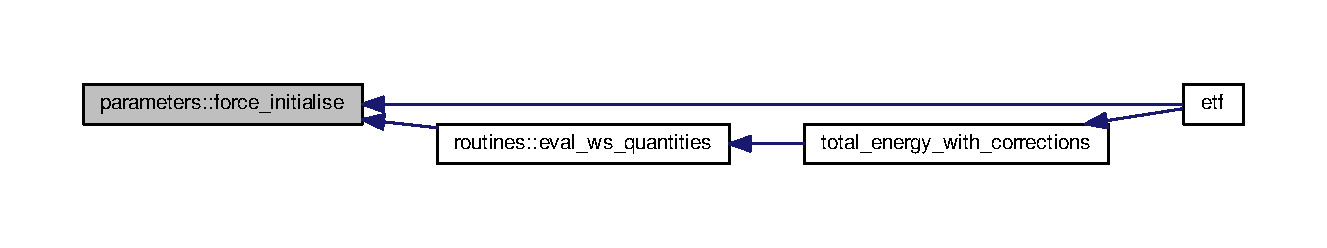
\includegraphics[width=350pt]{namespaceparameters_a55242f635842d12dbb53d66ae9248b93_icgraph}
\end{center}
\end{figure}


\subsection{Variable Documentation}
\mbox{\Hypertarget{namespaceparameters_a537af93b5aaa713688d624f145ebde80}\label{namespaceparameters_a537af93b5aaa713688d624f145ebde80}} 
\index{parameters@{parameters}!a\+\_\+q@{a\+\_\+q}}
\index{a\+\_\+q@{a\+\_\+q}!parameters@{parameters}}
\subsubsection{\texorpdfstring{a\+\_\+q}{a\_q}}
{\footnotesize\ttfamily real(kind=\mbox{\hyperlink{namespaceparameters_a52f8c6351fd79345d8811e065bcbbb37}{dp}}), dimension(\+:,\+:), allocatable parameters\+::a\+\_\+q}

\mbox{\Hypertarget{namespaceparameters_aaeb8117f8c15d7a7414e15929e12b0a8}\label{namespaceparameters_aaeb8117f8c15d7a7414e15929e12b0a8}} 
\index{parameters@{parameters}!d1\+\_\+a\+\_\+q@{d1\+\_\+a\+\_\+q}}
\index{d1\+\_\+a\+\_\+q@{d1\+\_\+a\+\_\+q}!parameters@{parameters}}
\subsubsection{\texorpdfstring{d1\+\_\+a\+\_\+q}{d1\_a\_q}}
{\footnotesize\ttfamily real(kind=\mbox{\hyperlink{namespaceparameters_a52f8c6351fd79345d8811e065bcbbb37}{dp}}), dimension(\+:,\+:), allocatable parameters\+::d1\+\_\+a\+\_\+q}

\mbox{\Hypertarget{namespaceparameters_ab2833e12dbfca51501df8955b00dd7d0}\label{namespaceparameters_ab2833e12dbfca51501df8955b00dd7d0}} 
\index{parameters@{parameters}!d2\+\_\+a\+\_\+q@{d2\+\_\+a\+\_\+q}}
\index{d2\+\_\+a\+\_\+q@{d2\+\_\+a\+\_\+q}!parameters@{parameters}}
\subsubsection{\texorpdfstring{d2\+\_\+a\+\_\+q}{d2\_a\_q}}
{\footnotesize\ttfamily real(kind=\mbox{\hyperlink{namespaceparameters_a52f8c6351fd79345d8811e065bcbbb37}{dp}}), dimension(\+:,\+:), allocatable parameters\+::d2\+\_\+a\+\_\+q}

\mbox{\Hypertarget{namespaceparameters_a4e57ed84b90c4ca5998a9cdaa8ccb2da}\label{namespaceparameters_a4e57ed84b90c4ca5998a9cdaa8ccb2da}} 
\index{parameters@{parameters}!d2\+\_\+f\+\_\+q@{d2\+\_\+f\+\_\+q}}
\index{d2\+\_\+f\+\_\+q@{d2\+\_\+f\+\_\+q}!parameters@{parameters}}
\subsubsection{\texorpdfstring{d2\+\_\+f\+\_\+q}{d2\_f\_q}}
{\footnotesize\ttfamily real(kind=\mbox{\hyperlink{namespaceparameters_a52f8c6351fd79345d8811e065bcbbb37}{dp}}), dimension(\+:,\+:), allocatable parameters\+::d2\+\_\+f\+\_\+q}

\mbox{\Hypertarget{namespaceparameters_a0234a871e1ff1d0be38099df82c5e698}\label{namespaceparameters_a0234a871e1ff1d0be38099df82c5e698}} 
\index{parameters@{parameters}!d2\+\_\+rho\+\_\+q@{d2\+\_\+rho\+\_\+q}}
\index{d2\+\_\+rho\+\_\+q@{d2\+\_\+rho\+\_\+q}!parameters@{parameters}}
\subsubsection{\texorpdfstring{d2\+\_\+rho\+\_\+q}{d2\_rho\_q}}
{\footnotesize\ttfamily real(kind=\mbox{\hyperlink{namespaceparameters_a52f8c6351fd79345d8811e065bcbbb37}{dp}}), dimension(\+:,\+:), allocatable parameters\+::d2\+\_\+rho\+\_\+q}

\mbox{\Hypertarget{namespaceparameters_a1449283e577e2769bd8bb5d57dbf1876}\label{namespaceparameters_a1449283e577e2769bd8bb5d57dbf1876}} 
\index{parameters@{parameters}!d3\+\_\+a\+\_\+q@{d3\+\_\+a\+\_\+q}}
\index{d3\+\_\+a\+\_\+q@{d3\+\_\+a\+\_\+q}!parameters@{parameters}}
\subsubsection{\texorpdfstring{d3\+\_\+a\+\_\+q}{d3\_a\_q}}
{\footnotesize\ttfamily real(kind=\mbox{\hyperlink{namespaceparameters_a52f8c6351fd79345d8811e065bcbbb37}{dp}}), dimension(\+:,\+:), allocatable parameters\+::d3\+\_\+a\+\_\+q}

\mbox{\Hypertarget{namespaceparameters_ada2cda17d0e9bccb3581a5b22a05f876}\label{namespaceparameters_ada2cda17d0e9bccb3581a5b22a05f876}} 
\index{parameters@{parameters}!d3\+\_\+f\+\_\+q@{d3\+\_\+f\+\_\+q}}
\index{d3\+\_\+f\+\_\+q@{d3\+\_\+f\+\_\+q}!parameters@{parameters}}
\subsubsection{\texorpdfstring{d3\+\_\+f\+\_\+q}{d3\_f\_q}}
{\footnotesize\ttfamily real(kind=\mbox{\hyperlink{namespaceparameters_a52f8c6351fd79345d8811e065bcbbb37}{dp}}), dimension(\+:,\+:), allocatable parameters\+::d3\+\_\+f\+\_\+q}

\mbox{\Hypertarget{namespaceparameters_a1621c80d10f0cca4fec0e20ffbdda0f5}\label{namespaceparameters_a1621c80d10f0cca4fec0e20ffbdda0f5}} 
\index{parameters@{parameters}!d3\+\_\+rho\+\_\+q@{d3\+\_\+rho\+\_\+q}}
\index{d3\+\_\+rho\+\_\+q@{d3\+\_\+rho\+\_\+q}!parameters@{parameters}}
\subsubsection{\texorpdfstring{d3\+\_\+rho\+\_\+q}{d3\_rho\_q}}
{\footnotesize\ttfamily real(kind=\mbox{\hyperlink{namespaceparameters_a52f8c6351fd79345d8811e065bcbbb37}{dp}}), dimension(\+:,\+:), allocatable parameters\+::d3\+\_\+rho\+\_\+q}

\mbox{\Hypertarget{namespaceparameters_a68e56fd9914d22072aed5a180c5a17b2}\label{namespaceparameters_a68e56fd9914d22072aed5a180c5a17b2}} 
\index{parameters@{parameters}!d4\+\_\+a\+\_\+q@{d4\+\_\+a\+\_\+q}}
\index{d4\+\_\+a\+\_\+q@{d4\+\_\+a\+\_\+q}!parameters@{parameters}}
\subsubsection{\texorpdfstring{d4\+\_\+a\+\_\+q}{d4\_a\_q}}
{\footnotesize\ttfamily real(kind=\mbox{\hyperlink{namespaceparameters_a52f8c6351fd79345d8811e065bcbbb37}{dp}}), dimension(\+:,\+:), allocatable parameters\+::d4\+\_\+a\+\_\+q}

\mbox{\Hypertarget{namespaceparameters_af226839e94cc06ff5d33f92af38a014c}\label{namespaceparameters_af226839e94cc06ff5d33f92af38a014c}} 
\index{parameters@{parameters}!d4\+\_\+f\+\_\+q@{d4\+\_\+f\+\_\+q}}
\index{d4\+\_\+f\+\_\+q@{d4\+\_\+f\+\_\+q}!parameters@{parameters}}
\subsubsection{\texorpdfstring{d4\+\_\+f\+\_\+q}{d4\_f\_q}}
{\footnotesize\ttfamily real(kind=\mbox{\hyperlink{namespaceparameters_a52f8c6351fd79345d8811e065bcbbb37}{dp}}), dimension(\+:,\+:), allocatable parameters\+::d4\+\_\+f\+\_\+q}

\mbox{\Hypertarget{namespaceparameters_a59deaa51eaa68f574d57f364fff6c77a}\label{namespaceparameters_a59deaa51eaa68f574d57f364fff6c77a}} 
\index{parameters@{parameters}!d4\+\_\+rho\+\_\+q@{d4\+\_\+rho\+\_\+q}}
\index{d4\+\_\+rho\+\_\+q@{d4\+\_\+rho\+\_\+q}!parameters@{parameters}}
\subsubsection{\texorpdfstring{d4\+\_\+rho\+\_\+q}{d4\_rho\_q}}
{\footnotesize\ttfamily real(kind=\mbox{\hyperlink{namespaceparameters_a52f8c6351fd79345d8811e065bcbbb37}{dp}}), dimension(\+:,\+:), allocatable parameters\+::d4\+\_\+rho\+\_\+q}

\mbox{\Hypertarget{namespaceparameters_ab8757a22096c3d5f05f0bf953b59dff4}\label{namespaceparameters_ab8757a22096c3d5f05f0bf953b59dff4}} 
\index{parameters@{parameters}!div\+\_\+j\+\_\+4\+\_\+q@{div\+\_\+j\+\_\+4\+\_\+q}}
\index{div\+\_\+j\+\_\+4\+\_\+q@{div\+\_\+j\+\_\+4\+\_\+q}!parameters@{parameters}}
\subsubsection{\texorpdfstring{div\+\_\+j\+\_\+4\+\_\+q}{div\_j\_4\_q}}
{\footnotesize\ttfamily real(kind=\mbox{\hyperlink{namespaceparameters_a52f8c6351fd79345d8811e065bcbbb37}{dp}}), dimension(\+:,\+:), allocatable parameters\+::div\+\_\+j\+\_\+4\+\_\+q}

\mbox{\Hypertarget{namespaceparameters_a52f8c6351fd79345d8811e065bcbbb37}\label{namespaceparameters_a52f8c6351fd79345d8811e065bcbbb37}} 
\index{parameters@{parameters}!dp@{dp}}
\index{dp@{dp}!parameters@{parameters}}
\subsubsection{\texorpdfstring{dp}{dp}}
{\footnotesize\ttfamily integer, parameter parameters\+::dp = selected\+\_\+real\+\_\+kind(15, 300)}



Precision. 

\mbox{\Hypertarget{namespaceparameters_a41689cc1fc405b2fd02236c39ee5528c}\label{namespaceparameters_a41689cc1fc405b2fd02236c39ee5528c}} 
\index{parameters@{parameters}!j\+\_\+4\+\_\+q@{j\+\_\+4\+\_\+q}}
\index{j\+\_\+4\+\_\+q@{j\+\_\+4\+\_\+q}!parameters@{parameters}}
\subsubsection{\texorpdfstring{j\+\_\+4\+\_\+q}{j\_4\_q}}
{\footnotesize\ttfamily real(kind=\mbox{\hyperlink{namespaceparameters_a52f8c6351fd79345d8811e065bcbbb37}{dp}}), dimension(\+:,\+:), allocatable parameters\+::j\+\_\+4\+\_\+q}

\mbox{\Hypertarget{namespaceparameters_a1dd9d0c60fab7b85157b61471151ed92}\label{namespaceparameters_a1dd9d0c60fab7b85157b61471151ed92}} 
\index{parameters@{parameters}!tau\+\_\+4\+\_\+cont\+\_\+q@{tau\+\_\+4\+\_\+cont\+\_\+q}}
\index{tau\+\_\+4\+\_\+cont\+\_\+q@{tau\+\_\+4\+\_\+cont\+\_\+q}!parameters@{parameters}}
\subsubsection{\texorpdfstring{tau\+\_\+4\+\_\+cont\+\_\+q}{tau\_4\_cont\_q}}
{\footnotesize\ttfamily real(kind=\mbox{\hyperlink{namespaceparameters_a52f8c6351fd79345d8811e065bcbbb37}{dp}}), dimension(\+:,\+:,\+:), allocatable parameters\+::tau\+\_\+4\+\_\+cont\+\_\+q}

\mbox{\Hypertarget{namespaceparameters_a6722d1e0c27f2796d4e43405bd9c9d81}\label{namespaceparameters_a6722d1e0c27f2796d4e43405bd9c9d81}} 
\index{parameters@{parameters}!tau\+\_\+4\+\_\+no\+\_\+spin\+\_\+q@{tau\+\_\+4\+\_\+no\+\_\+spin\+\_\+q}}
\index{tau\+\_\+4\+\_\+no\+\_\+spin\+\_\+q@{tau\+\_\+4\+\_\+no\+\_\+spin\+\_\+q}!parameters@{parameters}}
\subsubsection{\texorpdfstring{tau\+\_\+4\+\_\+no\+\_\+spin\+\_\+q}{tau\_4\_no\_spin\_q}}
{\footnotesize\ttfamily real(kind=\mbox{\hyperlink{namespaceparameters_a52f8c6351fd79345d8811e065bcbbb37}{dp}}), dimension(\+:,\+:), allocatable parameters\+::tau\+\_\+4\+\_\+no\+\_\+spin\+\_\+q}

\mbox{\Hypertarget{namespaceparameters_a6f95c2f318204d32f47cefa370021fe4}\label{namespaceparameters_a6f95c2f318204d32f47cefa370021fe4}} 
\index{parameters@{parameters}!tau\+\_\+4\+\_\+so\+\_\+q@{tau\+\_\+4\+\_\+so\+\_\+q}}
\index{tau\+\_\+4\+\_\+so\+\_\+q@{tau\+\_\+4\+\_\+so\+\_\+q}!parameters@{parameters}}
\subsubsection{\texorpdfstring{tau\+\_\+4\+\_\+so\+\_\+q}{tau\_4\_so\_q}}
{\footnotesize\ttfamily real(kind=\mbox{\hyperlink{namespaceparameters_a52f8c6351fd79345d8811e065bcbbb37}{dp}}), dimension(\+:,\+:), allocatable parameters\+::tau\+\_\+4\+\_\+so\+\_\+q}


\hypertarget{namespaceroutines}{}\section{routines Module Reference}
\label{namespaceroutines}\index{routines@{routines}}


Module to hold main routines\+: densities, energies.  


\subsection*{Functions/\+Subroutines}
\begin{DoxyCompactItemize}
\item 
integer function \mbox{\hyperlink{namespaceroutines_a8146fb4359e556bad19f882b8aabfc4b}{str2int}} (string)
\item 
subroutine \mbox{\hyperlink{namespaceroutines_a0d41e4cd4e61ac1463c75055bf784e8b}{allocate\+\_\+arrays}} ()
\begin{DoxyCompactList}\small\item\em Subroutine to allocate arrays for all densities and effective masses, and for their derivatives. \end{DoxyCompactList}\item 
subroutine \mbox{\hyperlink{namespaceroutines_a5caa9b33bdf3c960b6bb3bfa96771181}{initialise\+\_\+uniform\+\_\+mesh}} ()
\begin{DoxyCompactList}\small\item\em Subroutine to calculate number of mesh points for a uniform grid, allocate array for r, and then populate r with the mesh points. \end{DoxyCompactList}\item 
subroutine \mbox{\hyperlink{namespaceroutines_a27ad9ac802069004010c9759fecced92}{deallocate\+\_\+mesh}} ()
\begin{DoxyCompactList}\small\item\em Subroutine to deallocate array for r. \end{DoxyCompactList}\item 
subroutine \mbox{\hyperlink{namespaceroutines_ae7bc716d30ef4d9ecece5daa22324b77}{deallocate\+\_\+arrays}} ()
\begin{DoxyCompactList}\small\item\em Subroutine to deallocate arrays for all densities and effective masses, and for their derivatives. \end{DoxyCompactList}\item 
real(kind=dp) function \mbox{\hyperlink{namespaceroutines_a407a248748ce7c0e2e9e5dce03cc9415}{calc\+\_\+rho\+\_\+q}} (rhoqgas, rhoqliq, rq, aq, gammaq, r)
\begin{DoxyCompactList}\small\item\em Function to calculate the neutron or proton density at a given radius r, using supplied input parameters. \end{DoxyCompactList}\item 
subroutine \mbox{\hyperlink{namespaceroutines_a701f911aa939448c5bee0589d57369ca}{calc\+\_\+f\+\_\+q}} (rhot, rhoq, q, fq)
\begin{DoxyCompactList}\small\item\em Subroutine to calculate the effective mass ratio $f_q=\frac{m}{m^*_q}$ for neutrons or protons, for standard Skyrme or for B\+Sk forces. \end{DoxyCompactList}\item 
subroutine \mbox{\hyperlink{namespaceroutines_a8c520afea1e9ca6698a0792fbac37e7a}{calc\+\_\+w\+\_\+q}} (delrho, delrhoq, Wq)
\begin{DoxyCompactList}\small\item\em Function to calculate the spin-\/orbit field $\textbf{W}_q$ for neutrons or protons. \end{DoxyCompactList}\item 
subroutine \mbox{\hyperlink{namespaceroutines_a421a5d2cca448f46b0dfb9bcdeec1111}{calc\+\_\+tau\+\_\+tf}} (rhoq, tau\+TF)
\begin{DoxyCompactList}\small\item\em Function to calculate the zeroth-\/order contribution to the kinetic energy density for neutrons or protons. \end{DoxyCompactList}\item 
subroutine \mbox{\hyperlink{namespaceroutines_aaa80f6938f2b9c661821fa8956f8deef}{calc\+\_\+tau\+\_\+2\+\_\+l}} (rhoq, delrhoq, del2rhoq, tau2\+Lq, t2contq)
\begin{DoxyCompactList}\small\item\em Function to calculate the local second-\/order contribution to the kinetic energy density for neutrons or protons. \end{DoxyCompactList}\item 
subroutine \mbox{\hyperlink{namespaceroutines_a72bf2988651a9f3251dfb338ad1a7eca}{calc\+\_\+tau\+\_\+2\+\_\+nl}} (rhoq, delrhoq, fq, delfq, del2fq, Wq, q, tau2\+N\+Lq, t2contq)
\begin{DoxyCompactList}\small\item\em Subroutine to calculate the non-\/local second-\/order contribution to the kinetic energy density for neutrons or protons. \end{DoxyCompactList}\item 
subroutine \mbox{\hyperlink{namespaceroutines_a9c7e02754e0ae8816b1bfeab92df6bc8}{calc\+\_\+tau\+\_\+4\+\_\+no\+\_\+spin}} (rhoq, d1rhoq, d2rhoq, d3rhoq, d4rhoq, fq, d1fq, d2fq, d3fq, d4fq, tau4nospinq, t4contq)
\begin{DoxyCompactList}\small\item\em Subroutine to calculate the fourth-\/order contributions to the kinetic energy density (without spin-\/orbit contributions) $\textbf{tau}_q$ for neutrons or protons. \end{DoxyCompactList}\item 
subroutine \mbox{\hyperlink{namespaceroutines_a8825f02bb2ac98507fff5024d9b54c8f}{calc\+\_\+tau\+\_\+4\+\_\+so}} (rhoq, d1rhoq, fq, d1fq, d2fq, d1\+Aq, d2\+Aq, d3\+Aq, q, tau\+\_\+4\+\_\+so\+\_\+q, t4contq)
\begin{DoxyCompactList}\small\item\em Subroutine to calculate the fourth-\/order contributions to the kinetic energy density (spin-\/orbit contributions) $\textbf{tau}_q$ for neutrons or protons. \end{DoxyCompactList}\item 
subroutine \mbox{\hyperlink{namespaceroutines_af03f37f9deca52ef9a56287f50b982a1}{calc\+\_\+j\+\_\+2\+\_\+q}} (rhoq, Wq, fq, q, J2q)
\begin{DoxyCompactList}\small\item\em Subroutine to calculate the second-\/order contributions to the spin current density $\textbf{J}_q$ for neutrons or protons. \end{DoxyCompactList}\item 
subroutine \mbox{\hyperlink{namespaceroutines_a014fed5fe5fbc19302e7cbc651ba59bd}{calc\+\_\+j\+\_\+4\+\_\+q}} (rhoq, d1rhoq, fq, d1fq, d2fq, d1\+Aq, d2\+Aq, d3\+Aq, q, J4q)
\begin{DoxyCompactList}\small\item\em Subroutine to calculate the fourth-\/order contributions to the spin current density $\textbf{J}_q$ for neutrons or protons. \end{DoxyCompactList}\item 
subroutine \mbox{\hyperlink{namespaceroutines_a136b7a1f0387466390decb98ce91c152}{calc\+\_\+div\+\_\+j\+\_\+2\+\_\+q}} (rhoq, d1rhoq, fq, d1fq, d1\+Aq, d2\+Aq, q, div\+J2q)
\begin{DoxyCompactList}\small\item\em Subroutine to calculate the second-\/order contributions to the divergence of the current density $\textbf{J}_q$ for neutrons or protons. \end{DoxyCompactList}\item 
subroutine \mbox{\hyperlink{namespaceroutines_a7f66729f05be35eda4266dbf47eda026}{calc\+\_\+div\+\_\+j\+\_\+4\+\_\+q}} (rhoq, d1rhoq, d2rhoq, fq, d1fq, d2fq, d3fq, d1\+Aq, d2\+Aq, d3\+Aq, d4\+Aq, q, div\+J4q)
\begin{DoxyCompactList}\small\item\em Subroutine to calculate the fourth-\/order contributions to the divergence of the current density $\textbf{J}_q$ for neutrons or protons. \end{DoxyCompactList}\item 
real(kind=dp) function \mbox{\hyperlink{namespaceroutines_a2a44c591985c939162dabdeab4a4ced8}{calc\+\_\+u\+\_\+q}} (rhot, rhon, rhop, delrhot, delrhon, delrhop, del2rhot, del2rhon, del2rhop, taut, taun, taup, div\+Jt, div\+Jq, q)
\begin{DoxyCompactList}\small\item\em Function to calculate the central potential $U_q$ for neutrons or protons, for standard Skyrme or for B\+Sk forces with extra terms. \end{DoxyCompactList}\item 
subroutine \mbox{\hyperlink{namespaceroutines_aa995449a9eb9c404dbd756bdbea180a2}{eval\+\_\+fields}} ()
\begin{DoxyCompactList}\small\item\em Subroutine to evaluate matter density derivatives, and all fields\+: effective masses (and derivatives), spin-\/orbit fields, spin current densities (and derivatives) \end{DoxyCompactList}\item 
subroutine \mbox{\hyperlink{namespaceroutines_a97bfcff7e603cf9df3dcd48ae21b4612}{eval\+\_\+tau\+\_\+etf}} ()
\begin{DoxyCompactList}\small\item\em Subroutine to calculate the kinetic energy density $\tau_{ETF}$ with the (extended) Thomas-\/\+Fermi approximation at order specified by \char`\"{}etf\+\_\+order\char`\"{}. \end{DoxyCompactList}\item 
subroutine \mbox{\hyperlink{namespaceroutines_afb83677ec76758dadc35de4b01bac45c}{charge}} (rho, Neutr, Nprot, Ngrid1, del1, rhoch)
\begin{DoxyCompactList}\small\item\em Subroutine to calculate the charge density from the matter densities. Modified by M. Shelley. \end{DoxyCompactList}\item 
subroutine \mbox{\hyperlink{namespaceroutines_a74ed186c93b400a14428192e1cb7a0b2}{eval\+\_\+coulomb}} (prot\+\_\+dens, calc\+\_\+exchange)
\begin{DoxyCompactList}\small\item\em Subroutine to evaluate the Coulomb potentials and energy densities, using either the proton or charge density. \end{DoxyCompactList}\item 
subroutine \mbox{\hyperlink{namespaceroutines_a0b55cc503c7168299be63556e2602bd0}{eval\+\_\+electrons}} ()
\begin{DoxyCompactList}\small\item\em Subroutine to evaluate the proton-\/electron potential which contributes to $U_q$, all energy contributions, and the pressure, coming from a homogeneous electron gas. Also calculates the electron chemical potential. \end{DoxyCompactList}\item 
subroutine \mbox{\hyperlink{namespaceroutines_a6ee5e5cd7ce81b013d18b19f5f9a4092}{eval\+\_\+u\+\_\+q}} ()
\begin{DoxyCompactList}\small\item\em Subroutine to evaluate the central fields $U_q$. \end{DoxyCompactList}\item 
subroutine \mbox{\hyperlink{namespaceroutines_ae210968d134fbcc79297971cc4fefb82}{eval\+\_\+skyrme\+\_\+energy\+\_\+density}} ()
\begin{DoxyCompactList}\small\item\em Subroutine to evaluate the Skyrme energy density, after first separately evaluating the field energy density. \end{DoxyCompactList}\item 
subroutine \mbox{\hyperlink{namespaceroutines_a383e2bf5a1fa37fbf95dd5f6ddbcc6be}{pressure}} ()
\begin{DoxyCompactList}\small\item\em Subroutine to calculate the nuclear contribution to the pressure, and then the total pressure. \end{DoxyCompactList}\item 
subroutine \mbox{\hyperlink{namespaceroutines_a0b8346e8e5457d6befb48b0ac56f4fdf}{calc\+\_\+particle\+\_\+number}} ()
\begin{DoxyCompactList}\small\item\em Subroutine to calculate the number of particles in the Wigner-\/\+Seitz cell. \end{DoxyCompactList}\item 
subroutine \mbox{\hyperlink{namespaceroutines_a93de76f3b26ead66893f46dc4892dbcb}{eval\+\_\+ws\+\_\+quantities}} ()
\begin{DoxyCompactList}\small\item\em Subroutine to evaluate the various densities, fields, derivatives, energies, and particle numbers in the WS cell with densities $rho_q$. \end{DoxyCompactList}\item 
real(kind=dp) function \mbox{\hyperlink{namespaceroutines_a8f2a013c7bb06da429f995e288515248}{calc\+\_\+e\+\_\+f\+\_\+q}} (rhoq, fq, q)
\begin{DoxyCompactList}\small\item\em Subroutine to evaluate the Fermi energy at a given density and effective mass, for neutrons or protons. \end{DoxyCompactList}\item 
subroutine \mbox{\hyperlink{namespaceroutines_a92e52c281532c938dfa10d85404a367a}{d1}} (n, h, f, df)
\begin{DoxyCompactList}\small\item\em This subroutine computes the first derivative of function evaluated on the meshpoints 1,...,npt. The input is the function f with extrapolated values in -\/1, 0. Modified by M. Shelley. \end{DoxyCompactList}\item 
subroutine \mbox{\hyperlink{namespaceroutines_aafc8447e9af12216ae995f63c1606f1a}{d2}} (n, h, f, d2f)
\begin{DoxyCompactList}\small\item\em This subroutine computes the second derivative of function evaluated on the meshpoints 1,...,npt. The input is the function f with extrapolated values in -\/1, 0. Modified by M. Shelley. \end{DoxyCompactList}\item 
subroutine \mbox{\hyperlink{namespaceroutines_a635a2461a6c20207dd3b268842381ce3}{lap\+\_\+sphe\+\_\+symm}} (f, df\+\_\+dr, d2f\+\_\+dr2)
\begin{DoxyCompactList}\small\item\em Subroutine to carry out Laplacian in spherical symmetry. \end{DoxyCompactList}\item 
subroutine \mbox{\hyperlink{namespaceroutines_ac563b00969cb307d71ebc02aaef0a3b4}{d3}} (f, d3f\+\_\+dr3)
\begin{DoxyCompactList}\small\item\em Subroutine to calculate third derivative of function f evaluated on evenly-\/spaced meshpoints from 1 to n. Works with extrapolated values in -\/2,-\/1,0. Uses 7-\/point stencil. \end{DoxyCompactList}\item 
subroutine \mbox{\hyperlink{namespaceroutines_a6d38e9b19f2e939feb7840d2575fbb56}{d4}} (f, d4f\+\_\+dr4)
\begin{DoxyCompactList}\small\item\em Subroutine to calculate fourth derivative of function f evaluated on evenly-\/spaced meshpoints from 1 to n. Works with extrapolated values in -\/2,-\/1,0. Uses 7-\/point stencil. \end{DoxyCompactList}\item 
subroutine \mbox{\hyperlink{namespaceroutines_af143340288720f8019e944ec7110a84e}{extrapolate\+\_\+back\+\_\+3}} (grid)
\begin{DoxyCompactList}\small\item\em Subroutine to extrapolate back 3 points on the r mesh, to faciliate the calculation of first and second derivatives using a 5-\/point stencil. Values in grid start at 4, extrapolated values are put in elements 3,2,1. Coefficients come from solving 4th-\/order polynomial, assuming that f\textquotesingle{}(0) = 0, and f(-\/h) = f(h). \end{DoxyCompactList}\item 
real(kind=dp) function \mbox{\hyperlink{namespaceroutines_a5737b4327dcaa959a9ee519e4fca42e8}{ws\+\_\+integral}} (quantity, n\+\_\+max)
\begin{DoxyCompactList}\small\item\em Function to integrate a density or field over the whole W-\/S cell, using Simpson\textquotesingle{}s rule (+ Simpson\textquotesingle{}s 3/8 rule if odd number of points) \end{DoxyCompactList}\item 
subroutine \mbox{\hyperlink{namespaceroutines_a81e61269fb96b5478fd7140a1f185ec1}{write\+\_\+densities}} ()
\begin{DoxyCompactList}\small\item\em Subroutine to write neutron and proton densities to files. \end{DoxyCompactList}\item 
subroutine \mbox{\hyperlink{namespaceroutines_a4a59953c814b7fa48f2c4bf31d1763a2}{write\+\_\+fields}} ()
\begin{DoxyCompactList}\small\item\em Subroutine to write neutron and proton fields to files. \end{DoxyCompactList}\item 
subroutine \mbox{\hyperlink{namespaceroutines_ad51ac6c5da6056a5346d7b15b3fbe7b4}{write\+\_\+sp\+\_\+states\+\_\+p}} ()
\begin{DoxyCompactList}\small\item\em Subroutine to write proton single particle energies to file, and extra details if B\+CS has been performed. \end{DoxyCompactList}\end{DoxyCompactItemize}
\subsection*{Variables}
\begin{DoxyCompactItemize}
\item 
integer \mbox{\hyperlink{namespaceroutines_a4433ed4e6fbf0c81f38d8df1749be025}{file\+\_\+unit\+\_\+0}}
\item 
integer \mbox{\hyperlink{namespaceroutines_a806b34a65a0678e540be124100a0f908}{file\+\_\+unit\+\_\+1}}
\begin{DoxyCompactList}\small\item\em Unit numbers for opening files. \end{DoxyCompactList}\end{DoxyCompactItemize}


\subsection{Detailed Description}
Module to hold main routines\+: densities, energies. 

\begin{DoxyAuthor}{Author}
M. Shelley 
\end{DoxyAuthor}


\subsection{Function/\+Subroutine Documentation}
\mbox{\Hypertarget{namespaceroutines_a0d41e4cd4e61ac1463c75055bf784e8b}\label{namespaceroutines_a0d41e4cd4e61ac1463c75055bf784e8b}} 
\index{routines@{routines}!allocate\+\_\+arrays@{allocate\+\_\+arrays}}
\index{allocate\+\_\+arrays@{allocate\+\_\+arrays}!routines@{routines}}
\subsubsection{\texorpdfstring{allocate\+\_\+arrays()}{allocate\_arrays()}}
{\footnotesize\ttfamily subroutine routines\+::allocate\+\_\+arrays (\begin{DoxyParamCaption}{ }\end{DoxyParamCaption})}



Subroutine to allocate arrays for all densities and effective masses, and for their derivatives. 

\begin{DoxyAuthor}{Author}
M. Shelley 
\end{DoxyAuthor}
Here is the caller graph for this function\+:
\nopagebreak
\begin{figure}[H]
\begin{center}
\leavevmode
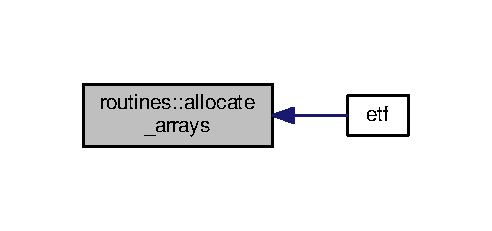
\includegraphics[width=236pt]{namespaceroutines_a0d41e4cd4e61ac1463c75055bf784e8b_icgraph}
\end{center}
\end{figure}
\mbox{\Hypertarget{namespaceroutines_a136b7a1f0387466390decb98ce91c152}\label{namespaceroutines_a136b7a1f0387466390decb98ce91c152}} 
\index{routines@{routines}!calc\+\_\+div\+\_\+j\+\_\+2\+\_\+q@{calc\+\_\+div\+\_\+j\+\_\+2\+\_\+q}}
\index{calc\+\_\+div\+\_\+j\+\_\+2\+\_\+q@{calc\+\_\+div\+\_\+j\+\_\+2\+\_\+q}!routines@{routines}}
\subsubsection{\texorpdfstring{calc\+\_\+div\+\_\+j\+\_\+2\+\_\+q()}{calc\_div\_j\_2\_q()}}
{\footnotesize\ttfamily subroutine routines\+::calc\+\_\+div\+\_\+j\+\_\+2\+\_\+q (\begin{DoxyParamCaption}\item[{real(kind=dp), dimension(1\+:n), intent(in)}]{rhoq,  }\item[{real(kind=dp), dimension(1\+:n), intent(in)}]{d1rhoq,  }\item[{real(kind=dp), dimension(1\+:n), intent(in)}]{fq,  }\item[{real(kind=dp), dimension(1\+:n), intent(in)}]{d1fq,  }\item[{real(kind=dp), dimension(1\+:n), intent(in)}]{d1\+Aq,  }\item[{real(kind=dp), dimension(1\+:n), intent(in)}]{d2\+Aq,  }\item[{integer, intent(in)}]{q,  }\item[{real(kind=dp), dimension(1\+:n), intent(inout)}]{div\+J2q }\end{DoxyParamCaption})}



Subroutine to calculate the second-\/order contributions to the divergence of the current density $\textbf{J}_q$ for neutrons or protons. 

\begin{DoxyAuthor}{Author}
M. Shelley 
\end{DoxyAuthor}

\begin{DoxyParams}[1]{Parameters}
\mbox{\tt in}  & {\em rhoq} & Neutron or proton density \\
\hline
\mbox{\tt in}  & {\em d1rhoq} & First derivative of neutron or proton density \\
\hline
\mbox{\tt in}  & {\em fq} & Effective mass for protons or neutrons \\
\hline
\mbox{\tt in}  & {\em d1fq} & First derivative of effective mass for neutrons or protons \\
\hline
\mbox{\tt in}  & {\em d1\+Aq} & First derivative of \char`\"{}composite\char`\"{} neutron or proton density $A_q$ \\
\hline
\mbox{\tt in}  & {\em d2\+Aq} & Second derivative of \char`\"{}composite\char`\"{} neutron or proton density $A_q$ \\
\hline
\mbox{\tt in}  & {\em q} & Isospin \\
\hline
\mbox{\tt in,out}  & {\em div\+J2q} & Array for second-\/order contributions \\
\hline
\end{DoxyParams}
Here is the caller graph for this function\+:
\nopagebreak
\begin{figure}[H]
\begin{center}
\leavevmode
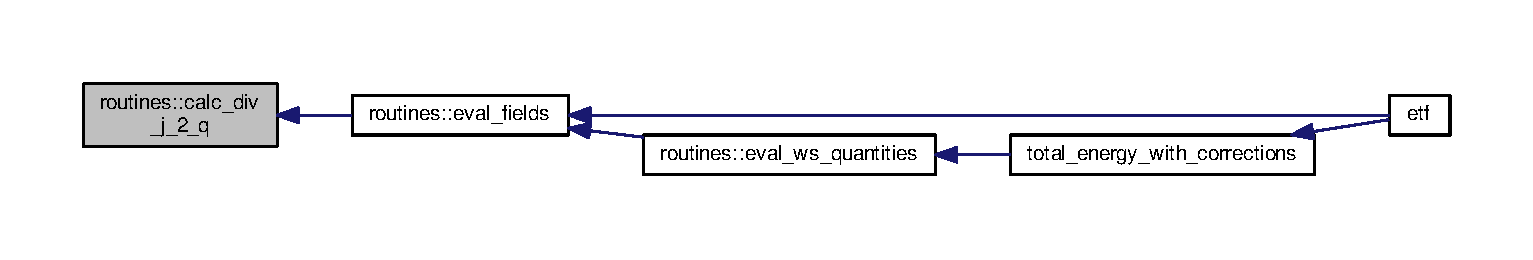
\includegraphics[width=350pt]{namespaceroutines_a136b7a1f0387466390decb98ce91c152_icgraph}
\end{center}
\end{figure}
\mbox{\Hypertarget{namespaceroutines_a7f66729f05be35eda4266dbf47eda026}\label{namespaceroutines_a7f66729f05be35eda4266dbf47eda026}} 
\index{routines@{routines}!calc\+\_\+div\+\_\+j\+\_\+4\+\_\+q@{calc\+\_\+div\+\_\+j\+\_\+4\+\_\+q}}
\index{calc\+\_\+div\+\_\+j\+\_\+4\+\_\+q@{calc\+\_\+div\+\_\+j\+\_\+4\+\_\+q}!routines@{routines}}
\subsubsection{\texorpdfstring{calc\+\_\+div\+\_\+j\+\_\+4\+\_\+q()}{calc\_div\_j\_4\_q()}}
{\footnotesize\ttfamily subroutine routines\+::calc\+\_\+div\+\_\+j\+\_\+4\+\_\+q (\begin{DoxyParamCaption}\item[{real(kind=dp), dimension(1\+:n), intent(in)}]{rhoq,  }\item[{real(kind=dp), dimension(1\+:n), intent(in)}]{d1rhoq,  }\item[{real(kind=dp), dimension(1\+:n), intent(in)}]{d2rhoq,  }\item[{real(kind=dp), dimension(1\+:n), intent(in)}]{fq,  }\item[{real(kind=dp), dimension(1\+:n), intent(in)}]{d1fq,  }\item[{real(kind=dp), dimension(1\+:n), intent(in)}]{d2fq,  }\item[{real(kind=dp), dimension(1\+:n), intent(in)}]{d3fq,  }\item[{real(kind=dp), dimension(1\+:n), intent(in)}]{d1\+Aq,  }\item[{real(kind=dp), dimension(1\+:n), intent(in)}]{d2\+Aq,  }\item[{real(kind=dp), dimension(1\+:n), intent(in)}]{d3\+Aq,  }\item[{real(kind=dp), dimension(1\+:n), intent(in)}]{d4\+Aq,  }\item[{integer, intent(in)}]{q,  }\item[{real(kind=dp), dimension(1\+:n), intent(inout)}]{div\+J4q }\end{DoxyParamCaption})}



Subroutine to calculate the fourth-\/order contributions to the divergence of the current density $\textbf{J}_q$ for neutrons or protons. 

\begin{DoxyAuthor}{Author}
M. Shelley 
\end{DoxyAuthor}

\begin{DoxyParams}[1]{Parameters}
\mbox{\tt in}  & {\em rhoq} & Neutron or proton density \\
\hline
\mbox{\tt in}  & {\em d1rhoq} & First derivative of neutron or proton density \\
\hline
\mbox{\tt in}  & {\em d2rhoq} & Second derivative of neutron or proton density \\
\hline
\mbox{\tt in}  & {\em fq} & Effective mass for protons or neutrons \\
\hline
\mbox{\tt in}  & {\em d1fq} & First derivative of effective mass for neutrons or protons \\
\hline
\mbox{\tt in}  & {\em d2fq} & Second derivative of effective mass for neutrons or protons \\
\hline
\mbox{\tt in}  & {\em d3fq} & Third derivative of effective mass for neutrons or protons \\
\hline
\mbox{\tt in}  & {\em d1\+Aq} & First derivative of \char`\"{}composite\char`\"{} neutron or proton density $A_q$ \\
\hline
\mbox{\tt in}  & {\em d2\+Aq} & Second derivative of \char`\"{}composite\char`\"{} neutron or proton density $A_q$ \\
\hline
\mbox{\tt in}  & {\em d3\+Aq} & Third derivative of \char`\"{}composite\char`\"{} neutron or proton density $A_q$ \\
\hline
\mbox{\tt in}  & {\em d4\+Aq} & Fourth derivative of \char`\"{}composite\char`\"{} neutron or proton density $A_q$ \\
\hline
\mbox{\tt in}  & {\em q} & Isospin \\
\hline
\mbox{\tt in,out}  & {\em div\+J4q} & Array for fourth-\/order contributions \\
\hline
\end{DoxyParams}
Here is the caller graph for this function\+:
\nopagebreak
\begin{figure}[H]
\begin{center}
\leavevmode
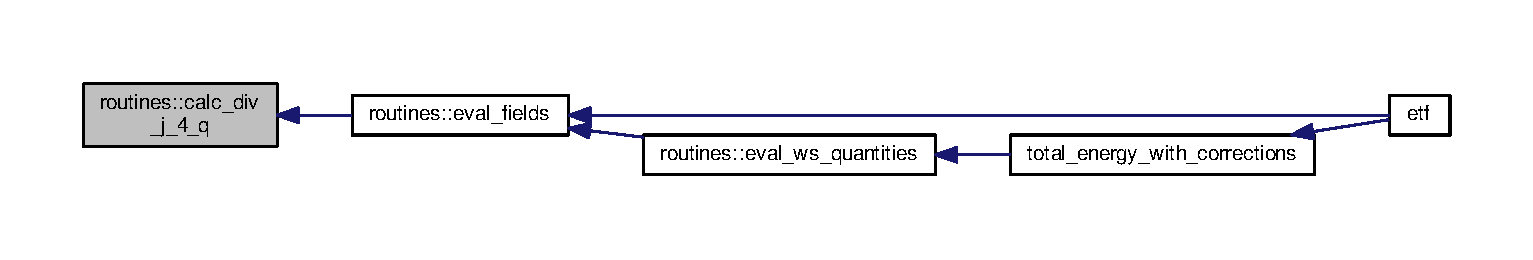
\includegraphics[width=350pt]{namespaceroutines_a7f66729f05be35eda4266dbf47eda026_icgraph}
\end{center}
\end{figure}
\mbox{\Hypertarget{namespaceroutines_a8f2a013c7bb06da429f995e288515248}\label{namespaceroutines_a8f2a013c7bb06da429f995e288515248}} 
\index{routines@{routines}!calc\+\_\+e\+\_\+f\+\_\+q@{calc\+\_\+e\+\_\+f\+\_\+q}}
\index{calc\+\_\+e\+\_\+f\+\_\+q@{calc\+\_\+e\+\_\+f\+\_\+q}!routines@{routines}}
\subsubsection{\texorpdfstring{calc\+\_\+e\+\_\+f\+\_\+q()}{calc\_e\_f\_q()}}
{\footnotesize\ttfamily real(kind=dp) function routines\+::calc\+\_\+e\+\_\+f\+\_\+q (\begin{DoxyParamCaption}\item[{real(kind=dp), intent(in)}]{rhoq,  }\item[{real(kind=dp), intent(in)}]{fq,  }\item[{integer, intent(in)}]{q }\end{DoxyParamCaption})}



Subroutine to evaluate the Fermi energy at a given density and effective mass, for neutrons or protons. 

\begin{DoxyAuthor}{Author}
M. Shelley 
\end{DoxyAuthor}

\begin{DoxyParams}[1]{Parameters}
\mbox{\tt in}  & {\em rhoq} & Neutron or proton density \\
\hline
\mbox{\tt in}  & {\em fn} & Neutron or proton effective mass \\
\hline
\end{DoxyParams}
Here is the caller graph for this function\+:
\nopagebreak
\begin{figure}[H]
\begin{center}
\leavevmode
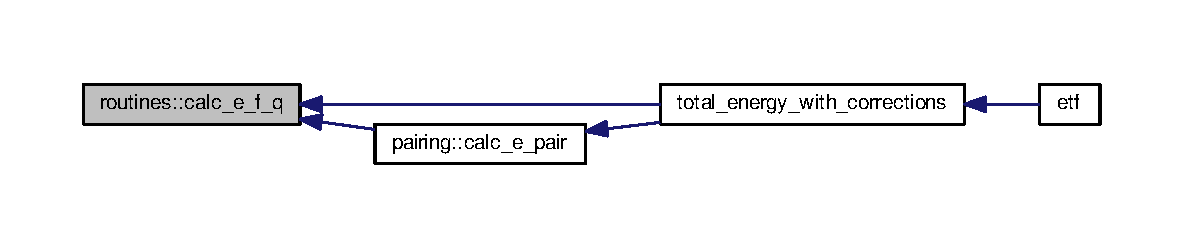
\includegraphics[width=350pt]{namespaceroutines_a8f2a013c7bb06da429f995e288515248_icgraph}
\end{center}
\end{figure}
\mbox{\Hypertarget{namespaceroutines_a701f911aa939448c5bee0589d57369ca}\label{namespaceroutines_a701f911aa939448c5bee0589d57369ca}} 
\index{routines@{routines}!calc\+\_\+f\+\_\+q@{calc\+\_\+f\+\_\+q}}
\index{calc\+\_\+f\+\_\+q@{calc\+\_\+f\+\_\+q}!routines@{routines}}
\subsubsection{\texorpdfstring{calc\+\_\+f\+\_\+q()}{calc\_f\_q()}}
{\footnotesize\ttfamily subroutine routines\+::calc\+\_\+f\+\_\+q (\begin{DoxyParamCaption}\item[{real(kind=dp), dimension(\+:), intent(in)}]{rhot,  }\item[{real(kind=dp), dimension(\+:), intent(in)}]{rhoq,  }\item[{integer, intent(in)}]{q,  }\item[{real(kind=dp), dimension(\+:), intent(inout)}]{fq }\end{DoxyParamCaption})}



Subroutine to calculate the effective mass ratio $f_q=\frac{m}{m^*_q}$ for neutrons or protons, for standard Skyrme or for B\+Sk forces. 

\begin{DoxyAuthor}{Author}
M. Shelley 
\end{DoxyAuthor}

\begin{DoxyParams}[1]{Parameters}
\mbox{\tt in}  & {\em rhot} & Total density \\
\hline
\mbox{\tt in}  & {\em rhoq} & Neutron or proton density \\
\hline
\mbox{\tt in}  & {\em q} & Isospin \\
\hline
\mbox{\tt in,out}  & {\em fq} & Neutron or proton effective mass \\
\hline
\end{DoxyParams}
Here is the call graph for this function\+:
\nopagebreak
\begin{figure}[H]
\begin{center}
\leavevmode
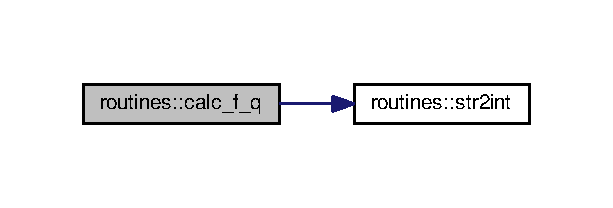
\includegraphics[width=294pt]{namespaceroutines_a701f911aa939448c5bee0589d57369ca_cgraph}
\end{center}
\end{figure}
Here is the caller graph for this function\+:
\nopagebreak
\begin{figure}[H]
\begin{center}
\leavevmode
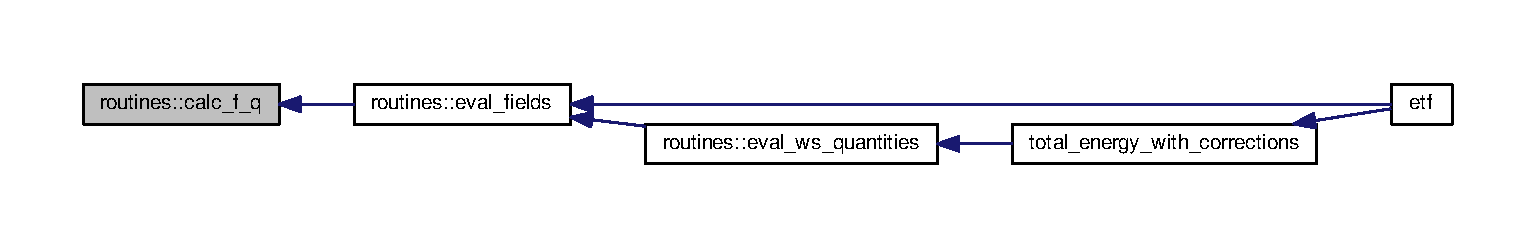
\includegraphics[width=350pt]{namespaceroutines_a701f911aa939448c5bee0589d57369ca_icgraph}
\end{center}
\end{figure}
\mbox{\Hypertarget{namespaceroutines_af03f37f9deca52ef9a56287f50b982a1}\label{namespaceroutines_af03f37f9deca52ef9a56287f50b982a1}} 
\index{routines@{routines}!calc\+\_\+j\+\_\+2\+\_\+q@{calc\+\_\+j\+\_\+2\+\_\+q}}
\index{calc\+\_\+j\+\_\+2\+\_\+q@{calc\+\_\+j\+\_\+2\+\_\+q}!routines@{routines}}
\subsubsection{\texorpdfstring{calc\+\_\+j\+\_\+2\+\_\+q()}{calc\_j\_2\_q()}}
{\footnotesize\ttfamily subroutine routines\+::calc\+\_\+j\+\_\+2\+\_\+q (\begin{DoxyParamCaption}\item[{real(kind=dp), dimension(1\+:n), intent(in)}]{rhoq,  }\item[{real(kind=dp), dimension(1\+:n), intent(in)}]{Wq,  }\item[{real(kind=dp), dimension(1\+:n), intent(in)}]{fq,  }\item[{integer, intent(in)}]{q,  }\item[{real(kind=dp), dimension(1\+:n), intent(inout)}]{J2q }\end{DoxyParamCaption})}



Subroutine to calculate the second-\/order contributions to the spin current density $\textbf{J}_q$ for neutrons or protons. 

\begin{DoxyAuthor}{Author}
M. Shelley 
\end{DoxyAuthor}

\begin{DoxyParams}[1]{Parameters}
\mbox{\tt in}  & {\em rhoq} & Neutron or proton density \\
\hline
\mbox{\tt in}  & {\em Wq} & Spin-\/orbit field \\
\hline
\mbox{\tt in}  & {\em fq} & Effective mass for neutrons or protons \\
\hline
\mbox{\tt in}  & {\em q} & Isospin \mbox{[}in,out\mbox{]} J2q Array for second-\/order contributions \\
\hline
\end{DoxyParams}
Here is the caller graph for this function\+:
\nopagebreak
\begin{figure}[H]
\begin{center}
\leavevmode
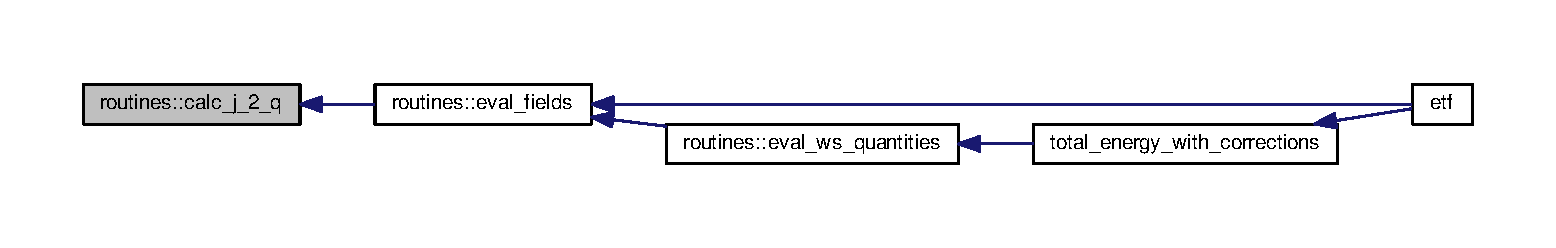
\includegraphics[width=350pt]{namespaceroutines_af03f37f9deca52ef9a56287f50b982a1_icgraph}
\end{center}
\end{figure}
\mbox{\Hypertarget{namespaceroutines_a014fed5fe5fbc19302e7cbc651ba59bd}\label{namespaceroutines_a014fed5fe5fbc19302e7cbc651ba59bd}} 
\index{routines@{routines}!calc\+\_\+j\+\_\+4\+\_\+q@{calc\+\_\+j\+\_\+4\+\_\+q}}
\index{calc\+\_\+j\+\_\+4\+\_\+q@{calc\+\_\+j\+\_\+4\+\_\+q}!routines@{routines}}
\subsubsection{\texorpdfstring{calc\+\_\+j\+\_\+4\+\_\+q()}{calc\_j\_4\_q()}}
{\footnotesize\ttfamily subroutine routines\+::calc\+\_\+j\+\_\+4\+\_\+q (\begin{DoxyParamCaption}\item[{real(kind=dp), dimension(1\+:n), intent(in)}]{rhoq,  }\item[{real(kind=dp), dimension(1\+:n), intent(in)}]{d1rhoq,  }\item[{real(kind=dp), dimension(1\+:n), intent(in)}]{fq,  }\item[{real(kind=dp), dimension(1\+:n), intent(in)}]{d1fq,  }\item[{real(kind=dp), dimension(1\+:n), intent(in)}]{d2fq,  }\item[{real(kind=dp), dimension(1\+:n), intent(in)}]{d1\+Aq,  }\item[{real(kind=dp), dimension(1\+:n), intent(in)}]{d2\+Aq,  }\item[{real(kind=dp), dimension(1\+:n), intent(in)}]{d3\+Aq,  }\item[{integer, intent(in)}]{q,  }\item[{real(kind=dp), dimension(1\+:n), intent(inout)}]{J4q }\end{DoxyParamCaption})}



Subroutine to calculate the fourth-\/order contributions to the spin current density $\textbf{J}_q$ for neutrons or protons. 

\begin{DoxyAuthor}{Author}
M. Shelley 
\end{DoxyAuthor}

\begin{DoxyParams}[1]{Parameters}
\mbox{\tt in}  & {\em rhoq} & Neutron or proton density \\
\hline
\mbox{\tt in}  & {\em d1rhoq} & First derivative of neutron or proton density \\
\hline
\mbox{\tt in}  & {\em fq} & Effective mass for protons or neutrons \\
\hline
\mbox{\tt in}  & {\em d1fq} & First derivative of effective mass for neutrons or protons \\
\hline
\mbox{\tt in}  & {\em d2fq} & Second derivative of effective mass for neutrons or protons \\
\hline
\mbox{\tt in}  & {\em d1\+Aq} & First derivative of \char`\"{}composite\char`\"{} neutron or proton density $A_q$ \\
\hline
\mbox{\tt in}  & {\em d2\+Aq} & Second derivative of \char`\"{}composite\char`\"{} neutron or proton density $A_q$ \\
\hline
\mbox{\tt in}  & {\em d3\+Aq} & Third derivative of \char`\"{}composite\char`\"{} neutron or proton density $A_q$ \\
\hline
\mbox{\tt in}  & {\em q} & Isospin \\
\hline
\mbox{\tt in,out}  & {\em J4q} & Array for fourth-\/order contributions \\
\hline
\end{DoxyParams}
Here is the caller graph for this function\+:
\nopagebreak
\begin{figure}[H]
\begin{center}
\leavevmode
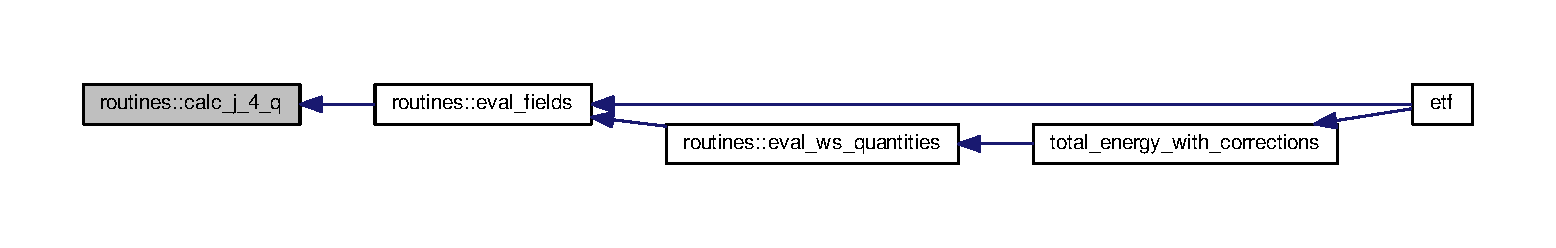
\includegraphics[width=350pt]{namespaceroutines_a014fed5fe5fbc19302e7cbc651ba59bd_icgraph}
\end{center}
\end{figure}
\mbox{\Hypertarget{namespaceroutines_a0b8346e8e5457d6befb48b0ac56f4fdf}\label{namespaceroutines_a0b8346e8e5457d6befb48b0ac56f4fdf}} 
\index{routines@{routines}!calc\+\_\+particle\+\_\+number@{calc\+\_\+particle\+\_\+number}}
\index{calc\+\_\+particle\+\_\+number@{calc\+\_\+particle\+\_\+number}!routines@{routines}}
\subsubsection{\texorpdfstring{calc\+\_\+particle\+\_\+number()}{calc\_particle\_number()}}
{\footnotesize\ttfamily subroutine routines\+::calc\+\_\+particle\+\_\+number (\begin{DoxyParamCaption}{ }\end{DoxyParamCaption})}



Subroutine to calculate the number of particles in the Wigner-\/\+Seitz cell. 

\begin{DoxyAuthor}{Author}
M. Shelley 
\end{DoxyAuthor}
Here is the call graph for this function\+:
\nopagebreak
\begin{figure}[H]
\begin{center}
\leavevmode
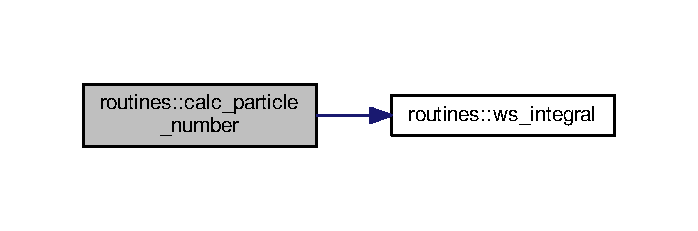
\includegraphics[width=335pt]{namespaceroutines_a0b8346e8e5457d6befb48b0ac56f4fdf_cgraph}
\end{center}
\end{figure}
Here is the caller graph for this function\+:
\nopagebreak
\begin{figure}[H]
\begin{center}
\leavevmode
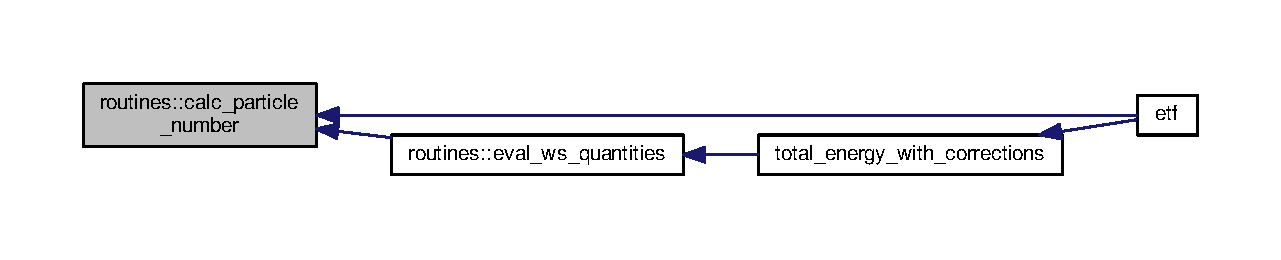
\includegraphics[width=350pt]{namespaceroutines_a0b8346e8e5457d6befb48b0ac56f4fdf_icgraph}
\end{center}
\end{figure}
\mbox{\Hypertarget{namespaceroutines_a407a248748ce7c0e2e9e5dce03cc9415}\label{namespaceroutines_a407a248748ce7c0e2e9e5dce03cc9415}} 
\index{routines@{routines}!calc\+\_\+rho\+\_\+q@{calc\+\_\+rho\+\_\+q}}
\index{calc\+\_\+rho\+\_\+q@{calc\+\_\+rho\+\_\+q}!routines@{routines}}
\subsubsection{\texorpdfstring{calc\+\_\+rho\+\_\+q()}{calc\_rho\_q()}}
{\footnotesize\ttfamily real(kind=dp) function routines\+::calc\+\_\+rho\+\_\+q (\begin{DoxyParamCaption}\item[{real(kind=dp), intent(in)}]{rhoqgas,  }\item[{real(kind=dp), intent(in)}]{rhoqliq,  }\item[{real(kind=dp), intent(in)}]{rq,  }\item[{real(kind=dp), intent(in)}]{aq,  }\item[{real(kind=dp), intent(in)}]{gammaq,  }\item[{real(kind=dp), intent(in)}]{r }\end{DoxyParamCaption})}



Function to calculate the neutron or proton density at a given radius r, using supplied input parameters. 

\begin{DoxyAuthor}{Author}
M. Shelley 
\end{DoxyAuthor}

\begin{DoxyParams}[1]{Parameters}
\mbox{\tt in}  & {\em rhoqgas} & Asymptotic density in gas far from surface \\
\hline
\mbox{\tt in}  & {\em rhoqliq} & Asymptotic density in cluster far from surface \\
\hline
\mbox{\tt in}  & {\em rq} & Cluster radius \\
\hline
\mbox{\tt in}  & {\em aq} & Surface diffuseness \\
\hline
\mbox{\tt in}  & {\em gammaq} & Parameter allowing for \char`\"{}asymmetric surface\char`\"{} \\
\hline
\mbox{\tt in}  & {\em r} & Radius \\
\hline
\end{DoxyParams}
Here is the caller graph for this function\+:
\nopagebreak
\begin{figure}[H]
\begin{center}
\leavevmode
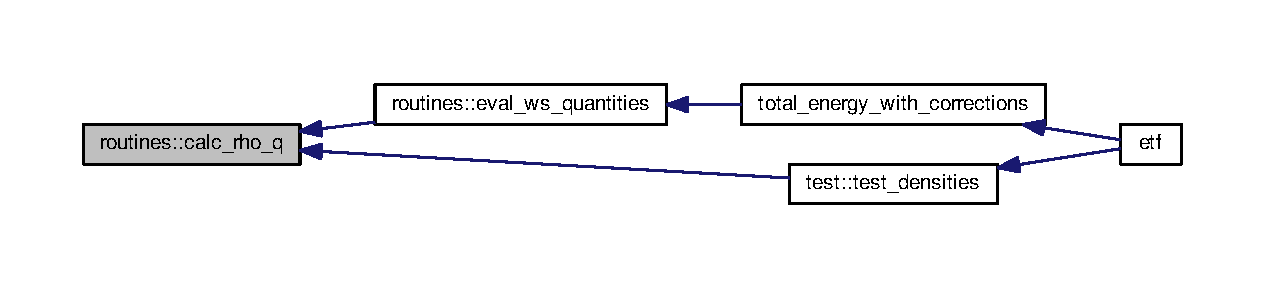
\includegraphics[width=350pt]{namespaceroutines_a407a248748ce7c0e2e9e5dce03cc9415_icgraph}
\end{center}
\end{figure}
\mbox{\Hypertarget{namespaceroutines_aaa80f6938f2b9c661821fa8956f8deef}\label{namespaceroutines_aaa80f6938f2b9c661821fa8956f8deef}} 
\index{routines@{routines}!calc\+\_\+tau\+\_\+2\+\_\+l@{calc\+\_\+tau\+\_\+2\+\_\+l}}
\index{calc\+\_\+tau\+\_\+2\+\_\+l@{calc\+\_\+tau\+\_\+2\+\_\+l}!routines@{routines}}
\subsubsection{\texorpdfstring{calc\+\_\+tau\+\_\+2\+\_\+l()}{calc\_tau\_2\_l()}}
{\footnotesize\ttfamily subroutine routines\+::calc\+\_\+tau\+\_\+2\+\_\+l (\begin{DoxyParamCaption}\item[{real(kind=dp), dimension(1\+:n), intent(in)}]{rhoq,  }\item[{real(kind=dp), dimension(1\+:n), intent(in)}]{delrhoq,  }\item[{real(kind=dp), dimension(1\+:n), intent(in)}]{del2rhoq,  }\item[{real(kind=dp), dimension(1\+:n), intent(inout)}]{tau2\+Lq,  }\item[{real(kind=dp), dimension(1\+:n), intent(inout)}]{t2contq }\end{DoxyParamCaption})}



Function to calculate the local second-\/order contribution to the kinetic energy density for neutrons or protons. 

\begin{DoxyAuthor}{Author}
M. Shelley 
\end{DoxyAuthor}

\begin{DoxyParams}[1]{Parameters}
\mbox{\tt in}  & {\em rhoq} & Neutron or proton density \\
\hline
\mbox{\tt in}  & {\em delrhoq} & Gradient of proton or neutron density \\
\hline
\mbox{\tt in}  & {\em del2rhoq} & Laplacian of proton or neutron density \\
\hline
\mbox{\tt in,out}  & {\em tau2\+Lq} & Array for local second-\/order contributions \\
\hline
\mbox{\tt in,out}  & {\em t2contq} & Array for individual second-\/order contributions \\
\hline
\end{DoxyParams}
Here is the caller graph for this function\+:
\nopagebreak
\begin{figure}[H]
\begin{center}
\leavevmode
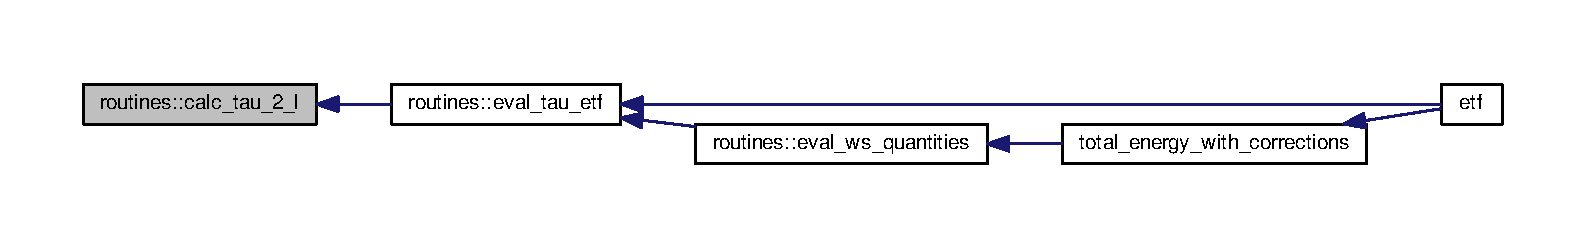
\includegraphics[width=350pt]{namespaceroutines_aaa80f6938f2b9c661821fa8956f8deef_icgraph}
\end{center}
\end{figure}
\mbox{\Hypertarget{namespaceroutines_a72bf2988651a9f3251dfb338ad1a7eca}\label{namespaceroutines_a72bf2988651a9f3251dfb338ad1a7eca}} 
\index{routines@{routines}!calc\+\_\+tau\+\_\+2\+\_\+nl@{calc\+\_\+tau\+\_\+2\+\_\+nl}}
\index{calc\+\_\+tau\+\_\+2\+\_\+nl@{calc\+\_\+tau\+\_\+2\+\_\+nl}!routines@{routines}}
\subsubsection{\texorpdfstring{calc\+\_\+tau\+\_\+2\+\_\+nl()}{calc\_tau\_2\_nl()}}
{\footnotesize\ttfamily subroutine routines\+::calc\+\_\+tau\+\_\+2\+\_\+nl (\begin{DoxyParamCaption}\item[{real(kind=dp), dimension(1\+:n), intent(in)}]{rhoq,  }\item[{real(kind=dp), dimension(1\+:n), intent(in)}]{delrhoq,  }\item[{real(kind=dp), dimension(1\+:n), intent(in)}]{fq,  }\item[{real(kind=dp), dimension(1\+:n), intent(in)}]{delfq,  }\item[{real(kind=dp), dimension(1\+:n), intent(in)}]{del2fq,  }\item[{real(kind=dp), dimension(1\+:n), intent(in)}]{Wq,  }\item[{integer, intent(in)}]{q,  }\item[{real(kind=dp), dimension(1\+:n), intent(inout)}]{tau2\+N\+Lq,  }\item[{real(kind=dp), dimension(1\+:n,2\+:4), intent(inout)}]{t2contq }\end{DoxyParamCaption})}



Subroutine to calculate the non-\/local second-\/order contribution to the kinetic energy density for neutrons or protons. 

\begin{DoxyAuthor}{Author}
M. Shelley 
\end{DoxyAuthor}

\begin{DoxyParams}[1]{Parameters}
\mbox{\tt in}  & {\em rhoq} & Neutron or proton density \\
\hline
\mbox{\tt in}  & {\em delrhoq} & Gradient of neutron or proton density \\
\hline
\mbox{\tt in}  & {\em fq} & Effective mass for neutrons or protons \\
\hline
\mbox{\tt in}  & {\em delfq} & Gradient of effective mass for neutrons or protons \\
\hline
\mbox{\tt in}  & {\em del2fq} & Laplacian of effective mass for neutrons or protons \\
\hline
\mbox{\tt in}  & {\em Wq} & Spin-\/orbit field \\
\hline
\mbox{\tt in}  & {\em q} & Isospin \\
\hline
\mbox{\tt in,out}  & {\em tau2\+N\+Lq} & Array for non-\/local second-\/order contributions \\
\hline
\mbox{\tt in,out}  & {\em t2contq} & Array for individual second-\/order contributions \\
\hline
\end{DoxyParams}
Here is the caller graph for this function\+:
\nopagebreak
\begin{figure}[H]
\begin{center}
\leavevmode
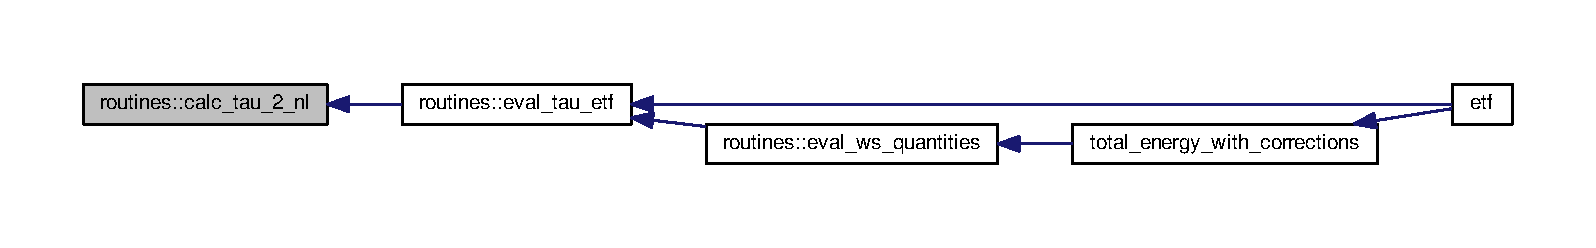
\includegraphics[width=350pt]{namespaceroutines_a72bf2988651a9f3251dfb338ad1a7eca_icgraph}
\end{center}
\end{figure}
\mbox{\Hypertarget{namespaceroutines_a9c7e02754e0ae8816b1bfeab92df6bc8}\label{namespaceroutines_a9c7e02754e0ae8816b1bfeab92df6bc8}} 
\index{routines@{routines}!calc\+\_\+tau\+\_\+4\+\_\+no\+\_\+spin@{calc\+\_\+tau\+\_\+4\+\_\+no\+\_\+spin}}
\index{calc\+\_\+tau\+\_\+4\+\_\+no\+\_\+spin@{calc\+\_\+tau\+\_\+4\+\_\+no\+\_\+spin}!routines@{routines}}
\subsubsection{\texorpdfstring{calc\+\_\+tau\+\_\+4\+\_\+no\+\_\+spin()}{calc\_tau\_4\_no\_spin()}}
{\footnotesize\ttfamily subroutine routines\+::calc\+\_\+tau\+\_\+4\+\_\+no\+\_\+spin (\begin{DoxyParamCaption}\item[{real(kind=dp), dimension(1\+:n), intent(in)}]{rhoq,  }\item[{real(kind=dp), dimension(1\+:n), intent(in)}]{d1rhoq,  }\item[{real(kind=dp), dimension(1\+:n), intent(in)}]{d2rhoq,  }\item[{real(kind=dp), dimension(1\+:n), intent(in)}]{d3rhoq,  }\item[{real(kind=dp), dimension(1\+:n), intent(in)}]{d4rhoq,  }\item[{real(kind=dp), dimension(1\+:n), intent(in)}]{fq,  }\item[{real(kind=dp), dimension(1\+:n), intent(in)}]{d1fq,  }\item[{real(kind=dp), dimension(1\+:n), intent(in)}]{d2fq,  }\item[{real(kind=dp), dimension(1\+:n), intent(in)}]{d3fq,  }\item[{real(kind=dp), dimension(1\+:n), intent(in)}]{d4fq,  }\item[{real(kind=dp), dimension(1\+:n), intent(inout)}]{tau4nospinq,  }\item[{real(kind=dp), dimension(1\+:n,1\+:3), intent(inout)}]{t4contq }\end{DoxyParamCaption})}



Subroutine to calculate the fourth-\/order contributions to the kinetic energy density (without spin-\/orbit contributions) $\textbf{tau}_q$ for neutrons or protons. 

\begin{DoxyAuthor}{Author}
M. Shelley 
\end{DoxyAuthor}

\begin{DoxyParams}[1]{Parameters}
\mbox{\tt in}  & {\em rhoq} & Neutron or proton density \\
\hline
\mbox{\tt in}  & {\em d1rhoq} & First derivative of neutron or proton density \\
\hline
\mbox{\tt in}  & {\em d2rhoq} & Second derivative of neutron or proton density \\
\hline
\mbox{\tt in}  & {\em d3rhoq} & Third derivative of neutron or proton density \\
\hline
\mbox{\tt in}  & {\em d4rhoq} & Fourth derivative of neutron or proton density \\
\hline
\mbox{\tt in}  & {\em fq} & Effective mass for neutrons or protons \\
\hline
\mbox{\tt in}  & {\em d1fq} & First derivative of effective mass for neutrons or protons \\
\hline
\mbox{\tt in}  & {\em d2fq} & Second derivative of effective mass for neutrons or protons \\
\hline
\mbox{\tt in}  & {\em d3fq} & Third derivative of effective mass for neutrons or protons \\
\hline
\mbox{\tt in}  & {\em d4fq} & Fourth derivative of effective mass for neutrons or protons \\
\hline
\mbox{\tt in,out}  & {\em tau4nospinq} & Array for fourth-\/order contributions (no spin-\/orbit) \\
\hline
\mbox{\tt in,out}  & {\em t4contq} & Array for individual fourth-\/order contributions \\
\hline
\end{DoxyParams}
Here is the caller graph for this function\+:
\nopagebreak
\begin{figure}[H]
\begin{center}
\leavevmode
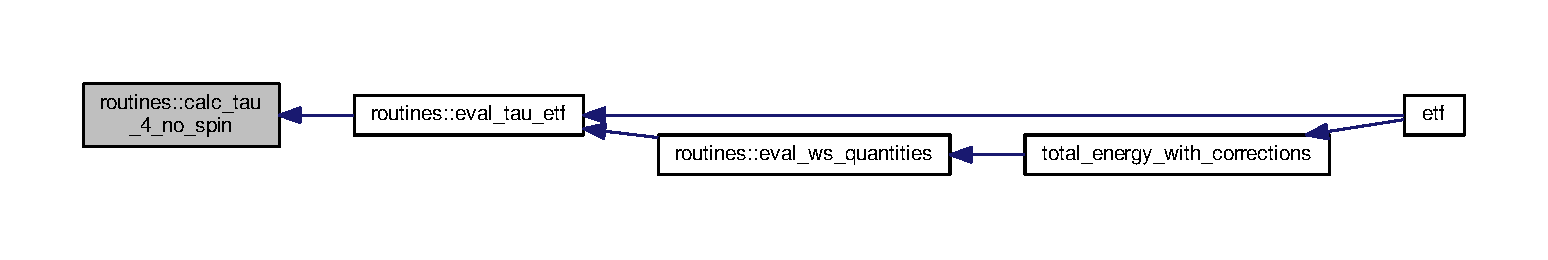
\includegraphics[width=350pt]{namespaceroutines_a9c7e02754e0ae8816b1bfeab92df6bc8_icgraph}
\end{center}
\end{figure}
\mbox{\Hypertarget{namespaceroutines_a8825f02bb2ac98507fff5024d9b54c8f}\label{namespaceroutines_a8825f02bb2ac98507fff5024d9b54c8f}} 
\index{routines@{routines}!calc\+\_\+tau\+\_\+4\+\_\+so@{calc\+\_\+tau\+\_\+4\+\_\+so}}
\index{calc\+\_\+tau\+\_\+4\+\_\+so@{calc\+\_\+tau\+\_\+4\+\_\+so}!routines@{routines}}
\subsubsection{\texorpdfstring{calc\+\_\+tau\+\_\+4\+\_\+so()}{calc\_tau\_4\_so()}}
{\footnotesize\ttfamily subroutine routines\+::calc\+\_\+tau\+\_\+4\+\_\+so (\begin{DoxyParamCaption}\item[{real(kind=dp), dimension(1\+:n), intent(in)}]{rhoq,  }\item[{real(kind=dp), dimension(1\+:n), intent(in)}]{d1rhoq,  }\item[{real(kind=dp), dimension(1\+:n), intent(in)}]{fq,  }\item[{real(kind=dp), dimension(1\+:n), intent(in)}]{d1fq,  }\item[{real(kind=dp), dimension(1\+:n), intent(in)}]{d2fq,  }\item[{real(kind=dp), dimension(1\+:n), intent(in)}]{d1\+Aq,  }\item[{real(kind=dp), dimension(1\+:n), intent(in)}]{d2\+Aq,  }\item[{real(kind=dp), dimension(1\+:n), intent(in)}]{d3\+Aq,  }\item[{integer, intent(in)}]{q,  }\item[{real(kind=dp), dimension(1\+:n), intent(inout)}]{tau\+\_\+4\+\_\+so\+\_\+q,  }\item[{real(kind=dp), dimension(1\+:n), intent(inout)}]{t4contq }\end{DoxyParamCaption})}



Subroutine to calculate the fourth-\/order contributions to the kinetic energy density (spin-\/orbit contributions) $\textbf{tau}_q$ for neutrons or protons. 

\begin{DoxyAuthor}{Author}
M. Shelley 
\end{DoxyAuthor}

\begin{DoxyParams}[1]{Parameters}
\mbox{\tt in}  & {\em rhoq} & Neutron or proton density \\
\hline
\mbox{\tt in}  & {\em d1rhoq} & First derivative of neutron or proton density \\
\hline
\mbox{\tt in}  & {\em fq} & Effective mass for protons or neutrons \\
\hline
\mbox{\tt in}  & {\em d1fq} & First derivative of effective mass for neutrons or protons \\
\hline
\mbox{\tt in}  & {\em d2fq} & Second derivative of effective mass for neutrons or protons \\
\hline
\mbox{\tt in}  & {\em d1\+Aq} & First derivative of \char`\"{}composite\char`\"{} neutron or proton density $A_q$ \\
\hline
\mbox{\tt in}  & {\em d2\+Aq} & Second derivative of \char`\"{}composite\char`\"{} neutron or proton density $A_q$ \\
\hline
\mbox{\tt in}  & {\em d3\+Aq} & Third derivative of \char`\"{}composite\char`\"{} neutron or proton density $A_q$ \\
\hline
\mbox{\tt in}  & {\em q} & Isospin \\
\hline
\mbox{\tt in,out}  & {\em tau\+\_\+4\+\_\+so\+\_\+q} & Array for fourth-\/order contributions (spin-\/ orbit) \\
\hline
\mbox{\tt in,out}  & {\em t4contq} & Array for individual fourth-\/order contributions \\
\hline
\end{DoxyParams}
Here is the caller graph for this function\+:
\nopagebreak
\begin{figure}[H]
\begin{center}
\leavevmode
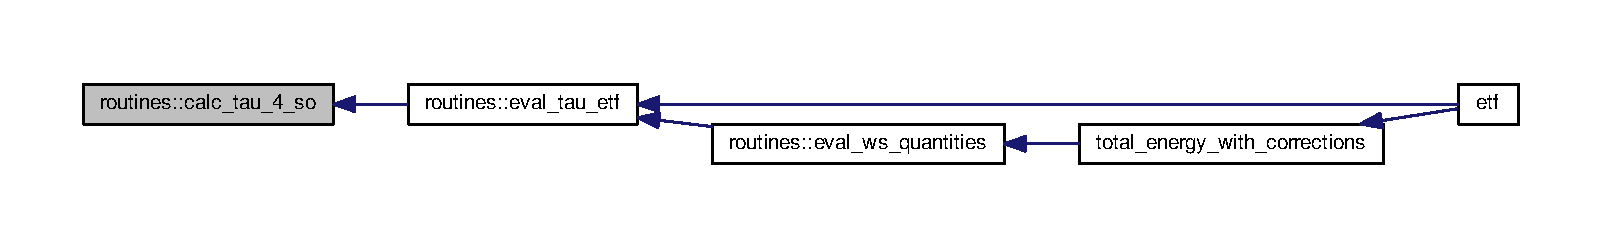
\includegraphics[width=350pt]{namespaceroutines_a8825f02bb2ac98507fff5024d9b54c8f_icgraph}
\end{center}
\end{figure}
\mbox{\Hypertarget{namespaceroutines_a421a5d2cca448f46b0dfb9bcdeec1111}\label{namespaceroutines_a421a5d2cca448f46b0dfb9bcdeec1111}} 
\index{routines@{routines}!calc\+\_\+tau\+\_\+tf@{calc\+\_\+tau\+\_\+tf}}
\index{calc\+\_\+tau\+\_\+tf@{calc\+\_\+tau\+\_\+tf}!routines@{routines}}
\subsubsection{\texorpdfstring{calc\+\_\+tau\+\_\+tf()}{calc\_tau\_tf()}}
{\footnotesize\ttfamily subroutine routines\+::calc\+\_\+tau\+\_\+tf (\begin{DoxyParamCaption}\item[{real(kind=dp), dimension(1\+:n), intent(in)}]{rhoq,  }\item[{real(kind=dp), dimension(1\+:n), intent(inout)}]{tau\+TF }\end{DoxyParamCaption})}



Function to calculate the zeroth-\/order contribution to the kinetic energy density for neutrons or protons. 

\begin{DoxyAuthor}{Author}
M. Shelley 
\end{DoxyAuthor}

\begin{DoxyParams}[1]{Parameters}
\mbox{\tt in}  & {\em rhoq} & Neutron or proton density \\
\hline
\mbox{\tt in,out}  & {\em tau\+TF} & Array for zeroth-\/order contributions \\
\hline
\end{DoxyParams}
Here is the caller graph for this function\+:
\nopagebreak
\begin{figure}[H]
\begin{center}
\leavevmode
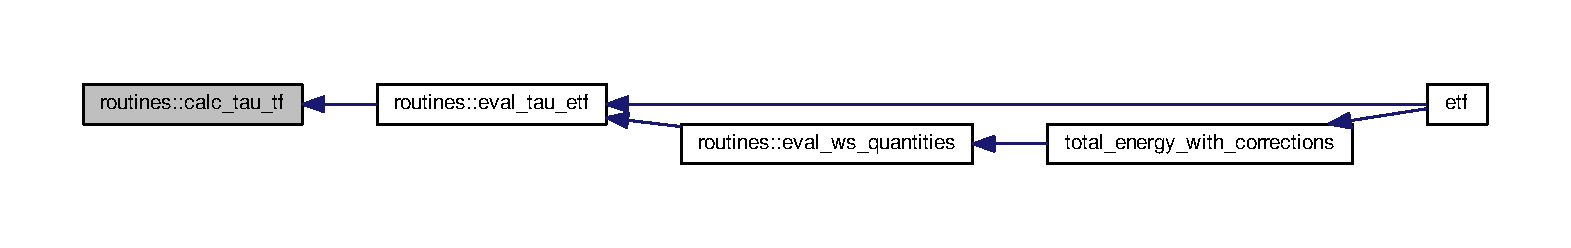
\includegraphics[width=350pt]{namespaceroutines_a421a5d2cca448f46b0dfb9bcdeec1111_icgraph}
\end{center}
\end{figure}
\mbox{\Hypertarget{namespaceroutines_a2a44c591985c939162dabdeab4a4ced8}\label{namespaceroutines_a2a44c591985c939162dabdeab4a4ced8}} 
\index{routines@{routines}!calc\+\_\+u\+\_\+q@{calc\+\_\+u\+\_\+q}}
\index{calc\+\_\+u\+\_\+q@{calc\+\_\+u\+\_\+q}!routines@{routines}}
\subsubsection{\texorpdfstring{calc\+\_\+u\+\_\+q()}{calc\_u\_q()}}
{\footnotesize\ttfamily real(kind=dp) function routines\+::calc\+\_\+u\+\_\+q (\begin{DoxyParamCaption}\item[{real(kind=dp), intent(in)}]{rhot,  }\item[{real(kind=dp), intent(in)}]{rhon,  }\item[{real(kind=dp), intent(in)}]{rhop,  }\item[{real(kind=dp), intent(in)}]{delrhot,  }\item[{real(kind=dp), intent(in)}]{delrhon,  }\item[{real(kind=dp), intent(in)}]{delrhop,  }\item[{real(kind=dp), intent(in)}]{del2rhot,  }\item[{real(kind=dp), intent(in)}]{del2rhon,  }\item[{real(kind=dp), intent(in)}]{del2rhop,  }\item[{real(kind=dp), intent(in)}]{taut,  }\item[{real(kind=dp), intent(in)}]{taun,  }\item[{real(kind=dp), intent(in)}]{taup,  }\item[{real(kind=dp), intent(in)}]{div\+Jt,  }\item[{real(kind=dp), intent(in)}]{div\+Jq,  }\item[{integer, intent(in)}]{q }\end{DoxyParamCaption})}



Function to calculate the central potential $U_q$ for neutrons or protons, for standard Skyrme or for B\+Sk forces with extra terms. 

\begin{DoxyAuthor}{Author}
M. Shelley 
\end{DoxyAuthor}

\begin{DoxyParams}[1]{Parameters}
\mbox{\tt in}  & {\em rhot} & Total density \\
\hline
\mbox{\tt in}  & {\em rhon} & Neutron density \\
\hline
\mbox{\tt in}  & {\em rhop} & Proton density \\
\hline
\mbox{\tt in}  & {\em delrhot} & First derivative of total density \\
\hline
\mbox{\tt in}  & {\em delrhon} & First derivative of neutron density \\
\hline
\mbox{\tt in}  & {\em delrhop} & First derivative of proton density \\
\hline
\mbox{\tt in}  & {\em del2rhot} & Laplacian of total density \\
\hline
\mbox{\tt in}  & {\em del2rhon} & Laplacian of neutron density \\
\hline
\mbox{\tt in}  & {\em del2rhop} & Laplacian of proton density \\
\hline
\mbox{\tt in}  & {\em taut} & Total kinetic density \\
\hline
\mbox{\tt in}  & {\em taun} & Neutron kinetic density \\
\hline
\mbox{\tt in}  & {\em taup} & Proton kinetic density \\
\hline
\mbox{\tt in}  & {\em div\+Jt} & Divergence of total spin current density \\
\hline
\mbox{\tt in}  & {\em div\+Jq} & Divergence of proton or neutron spin current density \\
\hline
\mbox{\tt in}  & {\em q} & Isospin \\
\hline
\end{DoxyParams}
Here is the call graph for this function\+:
\nopagebreak
\begin{figure}[H]
\begin{center}
\leavevmode
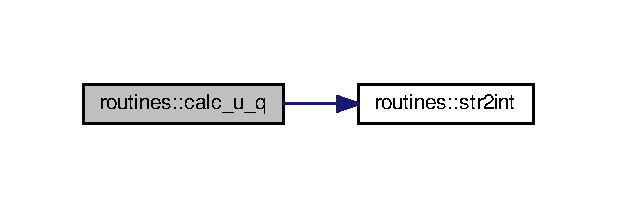
\includegraphics[width=296pt]{namespaceroutines_a2a44c591985c939162dabdeab4a4ced8_cgraph}
\end{center}
\end{figure}
Here is the caller graph for this function\+:
\nopagebreak
\begin{figure}[H]
\begin{center}
\leavevmode
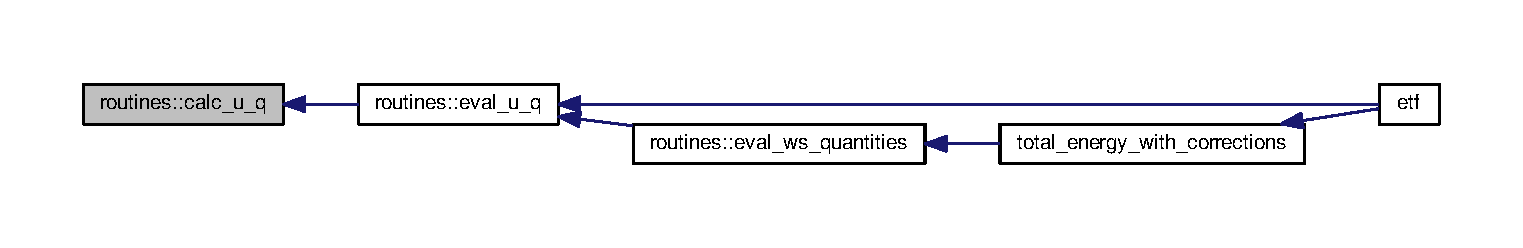
\includegraphics[width=350pt]{namespaceroutines_a2a44c591985c939162dabdeab4a4ced8_icgraph}
\end{center}
\end{figure}
\mbox{\Hypertarget{namespaceroutines_a8c520afea1e9ca6698a0792fbac37e7a}\label{namespaceroutines_a8c520afea1e9ca6698a0792fbac37e7a}} 
\index{routines@{routines}!calc\+\_\+w\+\_\+q@{calc\+\_\+w\+\_\+q}}
\index{calc\+\_\+w\+\_\+q@{calc\+\_\+w\+\_\+q}!routines@{routines}}
\subsubsection{\texorpdfstring{calc\+\_\+w\+\_\+q()}{calc\_w\_q()}}
{\footnotesize\ttfamily subroutine routines\+::calc\+\_\+w\+\_\+q (\begin{DoxyParamCaption}\item[{real(kind=dp), dimension(1\+:n), intent(in)}]{delrho,  }\item[{real(kind=dp), dimension(1\+:n), intent(in)}]{delrhoq,  }\item[{real(kind=dp), dimension(1\+:n), intent(inout)}]{Wq }\end{DoxyParamCaption})}



Function to calculate the spin-\/orbit field $\textbf{W}_q$ for neutrons or protons. 

\begin{DoxyAuthor}{Author}
M. Shelley 
\end{DoxyAuthor}

\begin{DoxyParams}[1]{Parameters}
\mbox{\tt in}  & {\em delrho} & Gradient of total density \\
\hline
\mbox{\tt in}  & {\em delrhoq} & Gradient of neutron or proton density \\
\hline
\mbox{\tt in,out}  & {\em Wq} & Array for spin-\/orbit field \\
\hline
\end{DoxyParams}
Here is the caller graph for this function\+:
\nopagebreak
\begin{figure}[H]
\begin{center}
\leavevmode
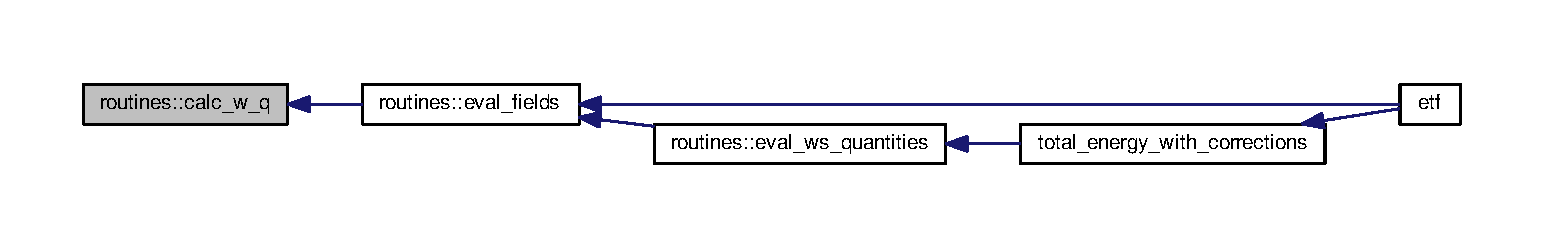
\includegraphics[width=350pt]{namespaceroutines_a8c520afea1e9ca6698a0792fbac37e7a_icgraph}
\end{center}
\end{figure}
\mbox{\Hypertarget{namespaceroutines_afb83677ec76758dadc35de4b01bac45c}\label{namespaceroutines_afb83677ec76758dadc35de4b01bac45c}} 
\index{routines@{routines}!charge@{charge}}
\index{charge@{charge}!routines@{routines}}
\subsubsection{\texorpdfstring{charge()}{charge()}}
{\footnotesize\ttfamily subroutine routines\+::charge (\begin{DoxyParamCaption}\item[{real(kind=dp), dimension(ngrid1,0\+:1), intent(in)}]{rho,  }\item[{real(kind=dp), intent(in)}]{Neutr,  }\item[{real(kind=dp), intent(in)}]{Nprot,  }\item[{integer, intent(in)}]{Ngrid1,  }\item[{real(kind=dp), intent(in)}]{del1,  }\item[{real(kind=dp), dimension(ngrid1), intent(inout)}]{rhoch }\end{DoxyParamCaption})}



Subroutine to calculate the charge density from the matter densities. Modified by M. Shelley. 

\begin{DoxyAuthor}{Author}
A. Pastore, M. Shelley 
\end{DoxyAuthor}

\begin{DoxyParams}[1]{Parameters}
\mbox{\tt in}  & {\em rho} & Neutron and proton densities \\
\hline
\mbox{\tt in}  & {\em Neutr} & Number of neutrons \\
\hline
\mbox{\tt in}  & {\em Nprot} & Number of protons \\
\hline
\mbox{\tt in}  & {\em Ngrid1} & Number of mesh points \\
\hline
\mbox{\tt in}  & {\em del1} & Step size \\
\hline
\mbox{\tt in,out}  & {\em rhoch} & Array for charge density \\
\hline
\end{DoxyParams}
Here is the caller graph for this function\+:
\nopagebreak
\begin{figure}[H]
\begin{center}
\leavevmode
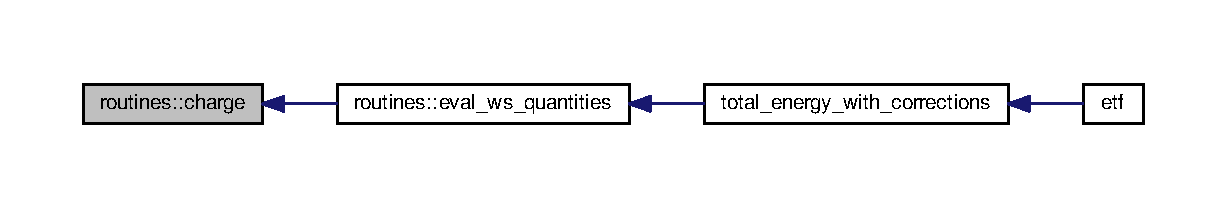
\includegraphics[width=350pt]{namespaceroutines_afb83677ec76758dadc35de4b01bac45c_icgraph}
\end{center}
\end{figure}
\mbox{\Hypertarget{namespaceroutines_a92e52c281532c938dfa10d85404a367a}\label{namespaceroutines_a92e52c281532c938dfa10d85404a367a}} 
\index{routines@{routines}!d1@{d1}}
\index{d1@{d1}!routines@{routines}}
\subsubsection{\texorpdfstring{d1()}{d1()}}
{\footnotesize\ttfamily subroutine routines\+::d1 (\begin{DoxyParamCaption}\item[{integer, intent(in)}]{n,  }\item[{real(kind=dp), intent(in)}]{h,  }\item[{real(kind=dp), dimension(-\/1\+:n), intent(in)}]{f,  }\item[{real(kind=dp), dimension(1\+:n), intent(inout)}]{df }\end{DoxyParamCaption})}



This subroutine computes the first derivative of function evaluated on the meshpoints 1,...,npt. The input is the function f with extrapolated values in -\/1, 0. Modified by M. Shelley. 

\begin{DoxyAuthor}{Author}
A. Pastore, M. Shelley 
\end{DoxyAuthor}

\begin{DoxyParams}[1]{Parameters}
\mbox{\tt in}  & {\em n} & Number of meshpoints \\
\hline
\mbox{\tt in}  & {\em f} & Input function (1\+:n) with extrapolated values in -\/1,0 \\
\hline
\mbox{\tt in}  & {\em h} & Step size \\
\hline
\mbox{\tt in,out}  & {\em df} & Array for first derivatives \\
\hline
\end{DoxyParams}
Here is the caller graph for this function\+:
\nopagebreak
\begin{figure}[H]
\begin{center}
\leavevmode
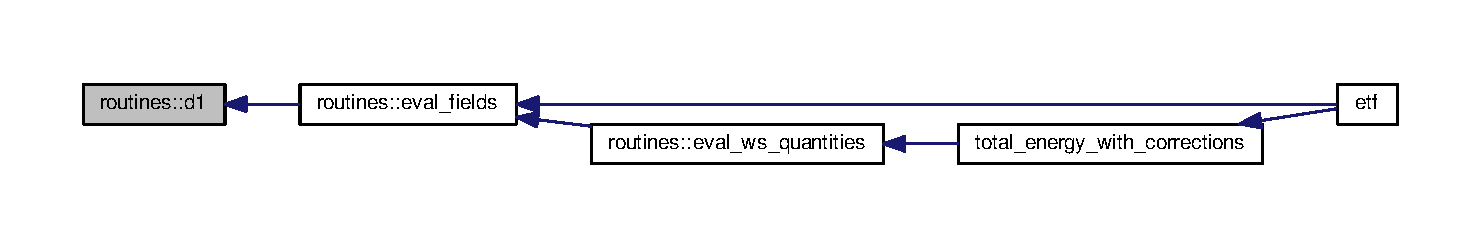
\includegraphics[width=350pt]{namespaceroutines_a92e52c281532c938dfa10d85404a367a_icgraph}
\end{center}
\end{figure}
\mbox{\Hypertarget{namespaceroutines_aafc8447e9af12216ae995f63c1606f1a}\label{namespaceroutines_aafc8447e9af12216ae995f63c1606f1a}} 
\index{routines@{routines}!d2@{d2}}
\index{d2@{d2}!routines@{routines}}
\subsubsection{\texorpdfstring{d2()}{d2()}}
{\footnotesize\ttfamily subroutine routines\+::d2 (\begin{DoxyParamCaption}\item[{integer, intent(in)}]{n,  }\item[{real(kind=dp), intent(in)}]{h,  }\item[{real(kind=dp), dimension(-\/1\+:n), intent(in)}]{f,  }\item[{real(kind=dp), dimension(1\+:n), intent(inout)}]{d2f }\end{DoxyParamCaption})}



This subroutine computes the second derivative of function evaluated on the meshpoints 1,...,npt. The input is the function f with extrapolated values in -\/1, 0. Modified by M. Shelley. 

\begin{DoxyAuthor}{Author}
A. Pastore, M. Shelley 
\end{DoxyAuthor}

\begin{DoxyParams}[1]{Parameters}
\mbox{\tt in}  & {\em n} & Number of meshpoints \\
\hline
\mbox{\tt in}  & {\em f} & Input function (1\+:n) with extrapolated values in -\/1,0 \\
\hline
\mbox{\tt in}  & {\em h} & Step size \\
\hline
\mbox{\tt in,out}  & {\em d2f} & Array for second derivatives \\
\hline
\end{DoxyParams}
Here is the caller graph for this function\+:
\nopagebreak
\begin{figure}[H]
\begin{center}
\leavevmode
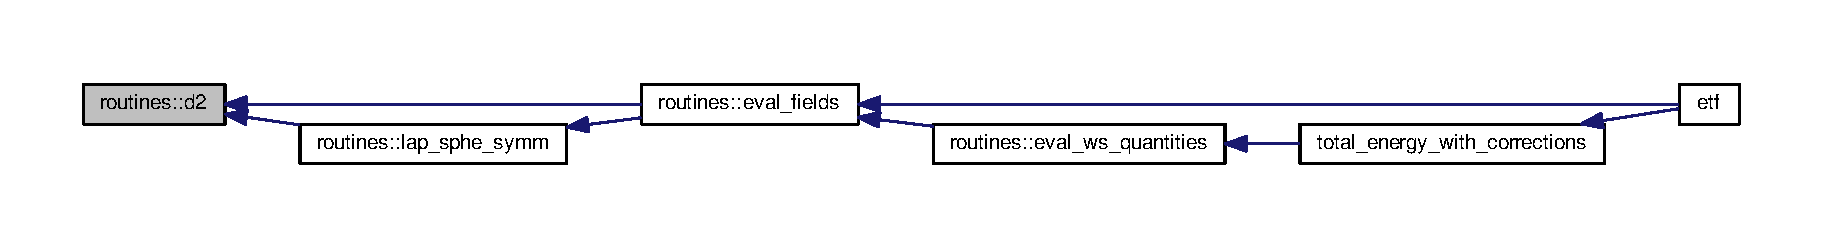
\includegraphics[width=350pt]{namespaceroutines_aafc8447e9af12216ae995f63c1606f1a_icgraph}
\end{center}
\end{figure}
\mbox{\Hypertarget{namespaceroutines_ac563b00969cb307d71ebc02aaef0a3b4}\label{namespaceroutines_ac563b00969cb307d71ebc02aaef0a3b4}} 
\index{routines@{routines}!d3@{d3}}
\index{d3@{d3}!routines@{routines}}
\subsubsection{\texorpdfstring{d3()}{d3()}}
{\footnotesize\ttfamily subroutine routines\+::d3 (\begin{DoxyParamCaption}\item[{real(kind=dp), dimension(-\/2\+:n), intent(in)}]{f,  }\item[{real(kind=dp), dimension(1\+:n), intent(inout)}]{d3f\+\_\+dr3 }\end{DoxyParamCaption})}



Subroutine to calculate third derivative of function f evaluated on evenly-\/spaced meshpoints from 1 to n. Works with extrapolated values in -\/2,-\/1,0. Uses 7-\/point stencil. 

\begin{DoxyAuthor}{Author}
M. Shelley 
\end{DoxyAuthor}

\begin{DoxyParams}[1]{Parameters}
\mbox{\tt in}  & {\em f} & Input function (1\+:n) with extrapolated values in -\/2,-\/1,0 \\
\hline
\mbox{\tt in,out}  & {\em d3f\+\_\+dr3} & Array for third derivative \\
\hline
\end{DoxyParams}
Here is the caller graph for this function\+:
\nopagebreak
\begin{figure}[H]
\begin{center}
\leavevmode
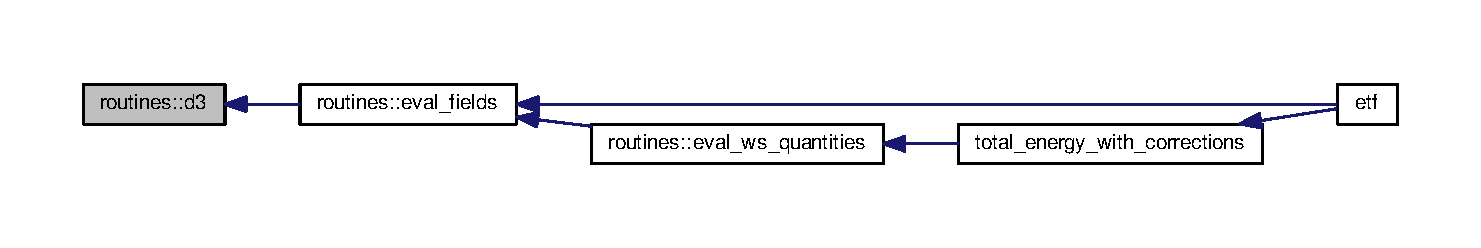
\includegraphics[width=350pt]{namespaceroutines_ac563b00969cb307d71ebc02aaef0a3b4_icgraph}
\end{center}
\end{figure}
\mbox{\Hypertarget{namespaceroutines_a6d38e9b19f2e939feb7840d2575fbb56}\label{namespaceroutines_a6d38e9b19f2e939feb7840d2575fbb56}} 
\index{routines@{routines}!d4@{d4}}
\index{d4@{d4}!routines@{routines}}
\subsubsection{\texorpdfstring{d4()}{d4()}}
{\footnotesize\ttfamily subroutine routines\+::d4 (\begin{DoxyParamCaption}\item[{real(kind=dp), dimension(-\/2\+:n), intent(in)}]{f,  }\item[{real(kind=dp), dimension(1\+:n), intent(inout)}]{d4f\+\_\+dr4 }\end{DoxyParamCaption})}



Subroutine to calculate fourth derivative of function f evaluated on evenly-\/spaced meshpoints from 1 to n. Works with extrapolated values in -\/2,-\/1,0. Uses 7-\/point stencil. 

\begin{DoxyAuthor}{Author}
M. Shelley 
\end{DoxyAuthor}

\begin{DoxyParams}[1]{Parameters}
\mbox{\tt in}  & {\em f} & Input function (1\+:n) with extrapolated values in -\/2,-\/1,0 \\
\hline
\mbox{\tt in,out}  & {\em d4f\+\_\+dr4} & Array for fourth derivative \\
\hline
\end{DoxyParams}
Here is the caller graph for this function\+:
\nopagebreak
\begin{figure}[H]
\begin{center}
\leavevmode
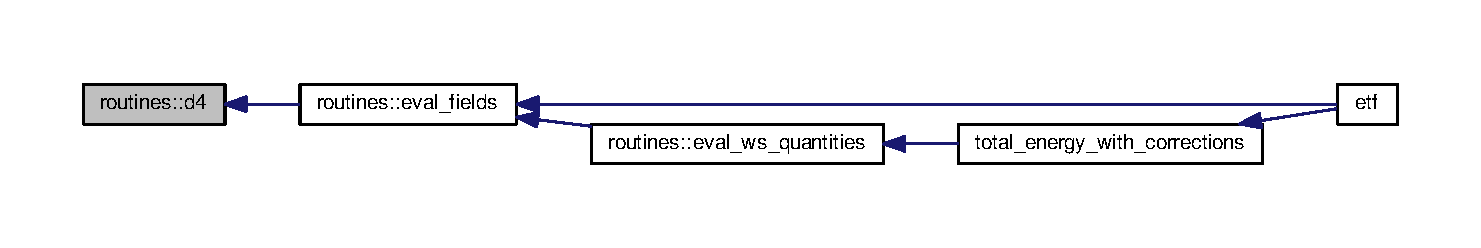
\includegraphics[width=350pt]{namespaceroutines_a6d38e9b19f2e939feb7840d2575fbb56_icgraph}
\end{center}
\end{figure}
\mbox{\Hypertarget{namespaceroutines_ae7bc716d30ef4d9ecece5daa22324b77}\label{namespaceroutines_ae7bc716d30ef4d9ecece5daa22324b77}} 
\index{routines@{routines}!deallocate\+\_\+arrays@{deallocate\+\_\+arrays}}
\index{deallocate\+\_\+arrays@{deallocate\+\_\+arrays}!routines@{routines}}
\subsubsection{\texorpdfstring{deallocate\+\_\+arrays()}{deallocate\_arrays()}}
{\footnotesize\ttfamily subroutine routines\+::deallocate\+\_\+arrays (\begin{DoxyParamCaption}{ }\end{DoxyParamCaption})}



Subroutine to deallocate arrays for all densities and effective masses, and for their derivatives. 

\begin{DoxyAuthor}{Author}
M. Shelley 
\end{DoxyAuthor}
Here is the caller graph for this function\+:
\nopagebreak
\begin{figure}[H]
\begin{center}
\leavevmode
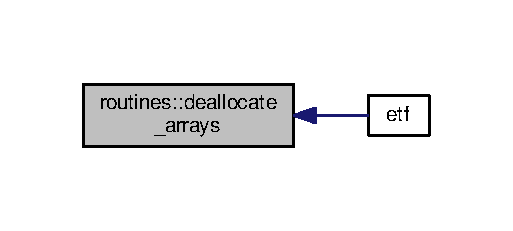
\includegraphics[width=246pt]{namespaceroutines_ae7bc716d30ef4d9ecece5daa22324b77_icgraph}
\end{center}
\end{figure}
\mbox{\Hypertarget{namespaceroutines_a27ad9ac802069004010c9759fecced92}\label{namespaceroutines_a27ad9ac802069004010c9759fecced92}} 
\index{routines@{routines}!deallocate\+\_\+mesh@{deallocate\+\_\+mesh}}
\index{deallocate\+\_\+mesh@{deallocate\+\_\+mesh}!routines@{routines}}
\subsubsection{\texorpdfstring{deallocate\+\_\+mesh()}{deallocate\_mesh()}}
{\footnotesize\ttfamily subroutine routines\+::deallocate\+\_\+mesh (\begin{DoxyParamCaption}{ }\end{DoxyParamCaption})}



Subroutine to deallocate array for r. 

\begin{DoxyAuthor}{Author}
M. Shelley 
\end{DoxyAuthor}
Here is the caller graph for this function\+:
\nopagebreak
\begin{figure}[H]
\begin{center}
\leavevmode
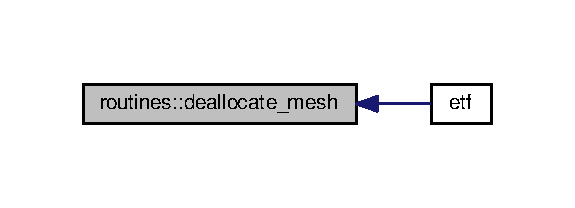
\includegraphics[width=276pt]{namespaceroutines_a27ad9ac802069004010c9759fecced92_icgraph}
\end{center}
\end{figure}
\mbox{\Hypertarget{namespaceroutines_a74ed186c93b400a14428192e1cb7a0b2}\label{namespaceroutines_a74ed186c93b400a14428192e1cb7a0b2}} 
\index{routines@{routines}!eval\+\_\+coulomb@{eval\+\_\+coulomb}}
\index{eval\+\_\+coulomb@{eval\+\_\+coulomb}!routines@{routines}}
\subsubsection{\texorpdfstring{eval\+\_\+coulomb()}{eval\_coulomb()}}
{\footnotesize\ttfamily subroutine routines\+::eval\+\_\+coulomb (\begin{DoxyParamCaption}\item[{real(kind=dp), dimension(1\+:n), intent(in)}]{prot\+\_\+dens,  }\item[{logical, intent(in)}]{calc\+\_\+exchange }\end{DoxyParamCaption})}



Subroutine to evaluate the Coulomb potentials and energy densities, using either the proton or charge density. 

\begin{DoxyAuthor}{Author}
M. Shelley 
\end{DoxyAuthor}

\begin{DoxyParams}[1]{Parameters}
\mbox{\tt in}  & {\em prot\+\_\+dens} & Density to use (proton or charge) \\
\hline
\mbox{\tt in}  & {\em calc\+\_\+exchange} & Whether to calculate exchange potential \\
\hline
\end{DoxyParams}
Here is the call graph for this function\+:
\nopagebreak
\begin{figure}[H]
\begin{center}
\leavevmode
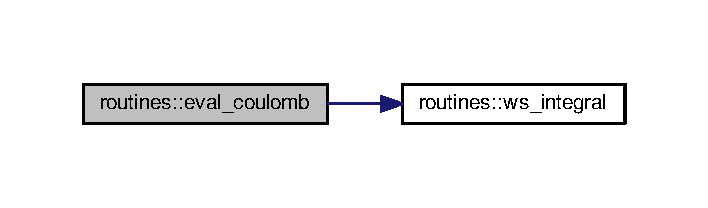
\includegraphics[width=340pt]{namespaceroutines_a74ed186c93b400a14428192e1cb7a0b2_cgraph}
\end{center}
\end{figure}
Here is the caller graph for this function\+:
\nopagebreak
\begin{figure}[H]
\begin{center}
\leavevmode
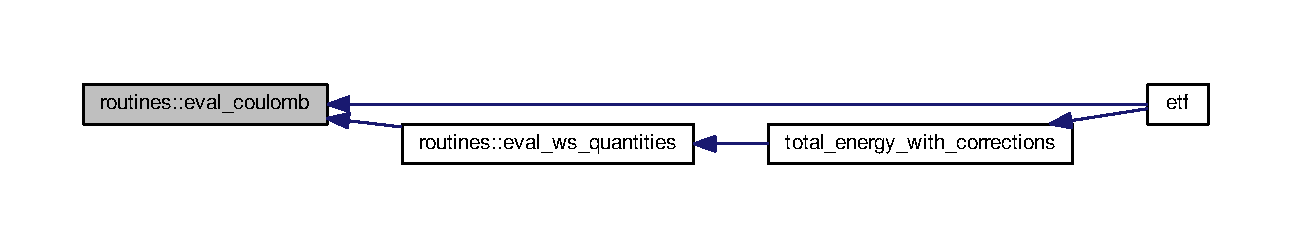
\includegraphics[width=350pt]{namespaceroutines_a74ed186c93b400a14428192e1cb7a0b2_icgraph}
\end{center}
\end{figure}
\mbox{\Hypertarget{namespaceroutines_a0b55cc503c7168299be63556e2602bd0}\label{namespaceroutines_a0b55cc503c7168299be63556e2602bd0}} 
\index{routines@{routines}!eval\+\_\+electrons@{eval\+\_\+electrons}}
\index{eval\+\_\+electrons@{eval\+\_\+electrons}!routines@{routines}}
\subsubsection{\texorpdfstring{eval\+\_\+electrons()}{eval\_electrons()}}
{\footnotesize\ttfamily subroutine routines\+::eval\+\_\+electrons (\begin{DoxyParamCaption}{ }\end{DoxyParamCaption})}



Subroutine to evaluate the proton-\/electron potential which contributes to $U_q$, all energy contributions, and the pressure, coming from a homogeneous electron gas. Also calculates the electron chemical potential. 

\begin{DoxyAuthor}{Author}
M. Shelley 
\end{DoxyAuthor}
Here is the call graph for this function\+:
\nopagebreak
\begin{figure}[H]
\begin{center}
\leavevmode
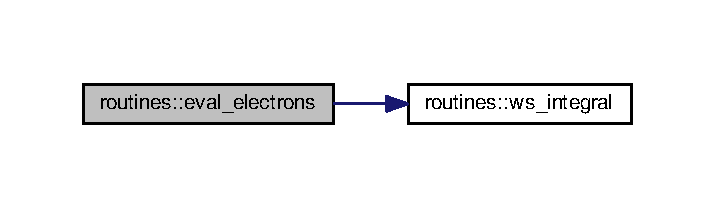
\includegraphics[width=343pt]{namespaceroutines_a0b55cc503c7168299be63556e2602bd0_cgraph}
\end{center}
\end{figure}
Here is the caller graph for this function\+:
\nopagebreak
\begin{figure}[H]
\begin{center}
\leavevmode
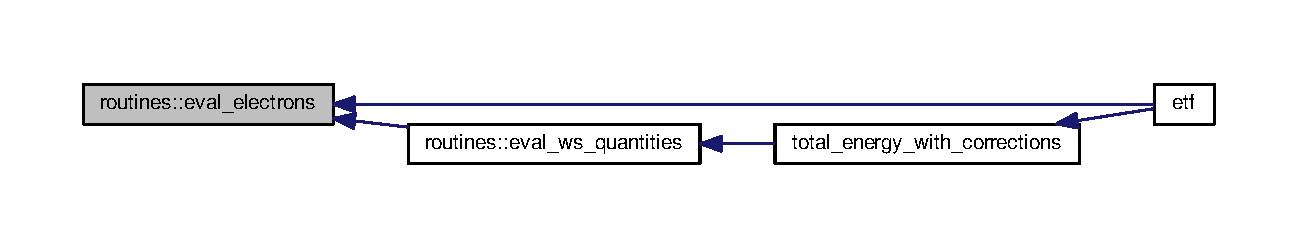
\includegraphics[width=350pt]{namespaceroutines_a0b55cc503c7168299be63556e2602bd0_icgraph}
\end{center}
\end{figure}
\mbox{\Hypertarget{namespaceroutines_aa995449a9eb9c404dbd756bdbea180a2}\label{namespaceroutines_aa995449a9eb9c404dbd756bdbea180a2}} 
\index{routines@{routines}!eval\+\_\+fields@{eval\+\_\+fields}}
\index{eval\+\_\+fields@{eval\+\_\+fields}!routines@{routines}}
\subsubsection{\texorpdfstring{eval\+\_\+fields()}{eval\_fields()}}
{\footnotesize\ttfamily subroutine routines\+::eval\+\_\+fields (\begin{DoxyParamCaption}{ }\end{DoxyParamCaption})}



Subroutine to evaluate matter density derivatives, and all fields\+: effective masses (and derivatives), spin-\/orbit fields, spin current densities (and derivatives) 

\begin{DoxyAuthor}{Author}
M. Shelley 
\end{DoxyAuthor}
Here is the call graph for this function\+:
\nopagebreak
\begin{figure}[H]
\begin{center}
\leavevmode
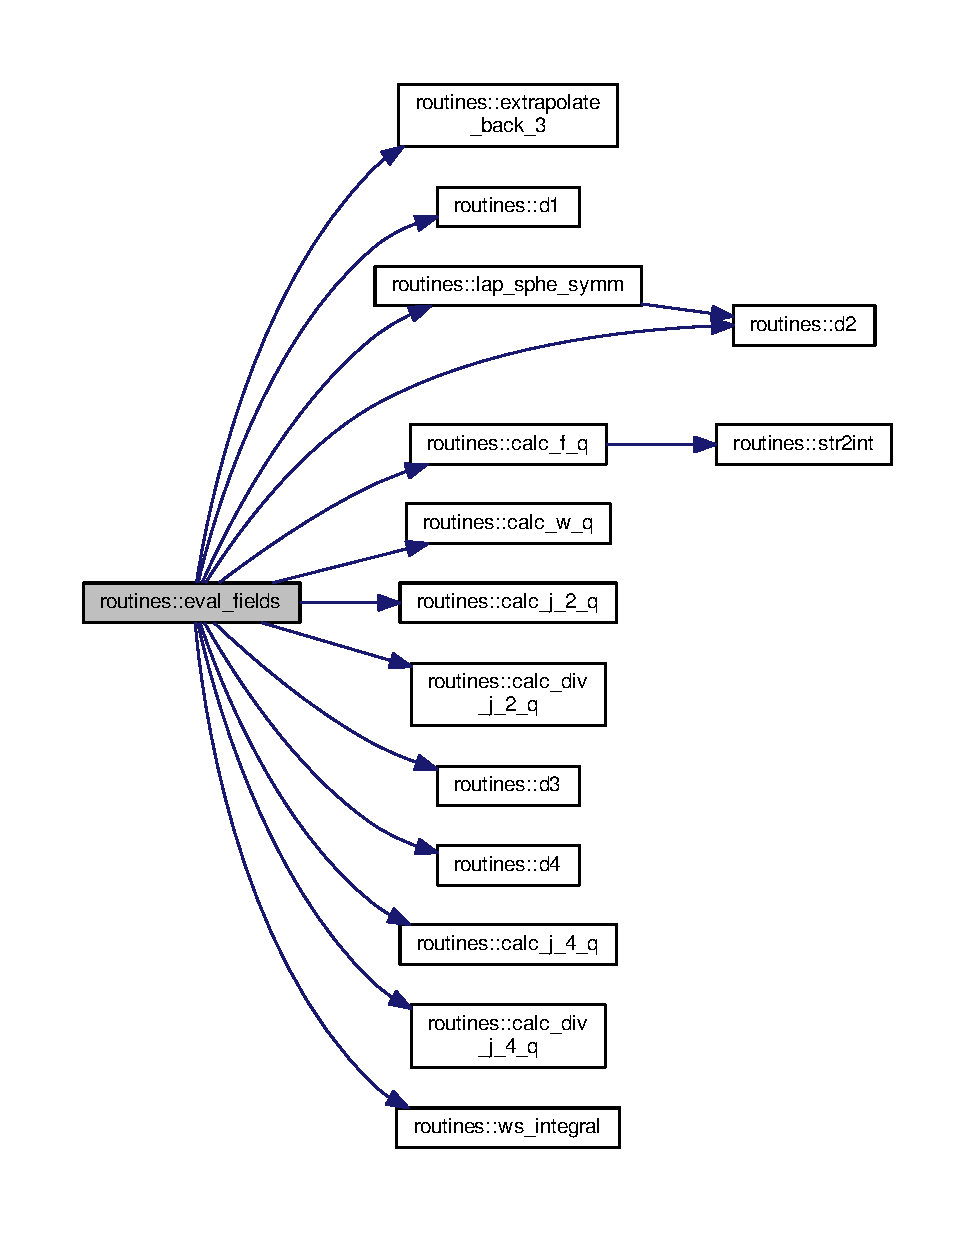
\includegraphics[width=350pt]{namespaceroutines_aa995449a9eb9c404dbd756bdbea180a2_cgraph}
\end{center}
\end{figure}
Here is the caller graph for this function\+:
\nopagebreak
\begin{figure}[H]
\begin{center}
\leavevmode
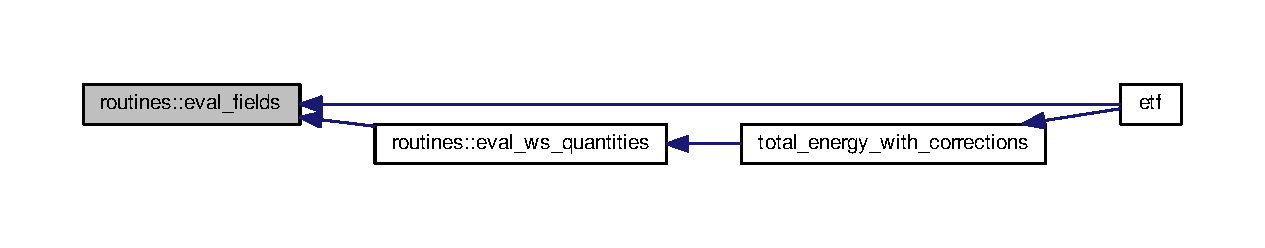
\includegraphics[width=350pt]{namespaceroutines_aa995449a9eb9c404dbd756bdbea180a2_icgraph}
\end{center}
\end{figure}
\mbox{\Hypertarget{namespaceroutines_ae210968d134fbcc79297971cc4fefb82}\label{namespaceroutines_ae210968d134fbcc79297971cc4fefb82}} 
\index{routines@{routines}!eval\+\_\+skyrme\+\_\+energy\+\_\+density@{eval\+\_\+skyrme\+\_\+energy\+\_\+density}}
\index{eval\+\_\+skyrme\+\_\+energy\+\_\+density@{eval\+\_\+skyrme\+\_\+energy\+\_\+density}!routines@{routines}}
\subsubsection{\texorpdfstring{eval\+\_\+skyrme\+\_\+energy\+\_\+density()}{eval\_skyrme\_energy\_density()}}
{\footnotesize\ttfamily subroutine routines\+::eval\+\_\+skyrme\+\_\+energy\+\_\+density (\begin{DoxyParamCaption}{ }\end{DoxyParamCaption})}



Subroutine to evaluate the Skyrme energy density, after first separately evaluating the field energy density. 

\begin{DoxyAuthor}{Author}
M. Shelley 
\end{DoxyAuthor}
Here is the call graph for this function\+:
\nopagebreak
\begin{figure}[H]
\begin{center}
\leavevmode
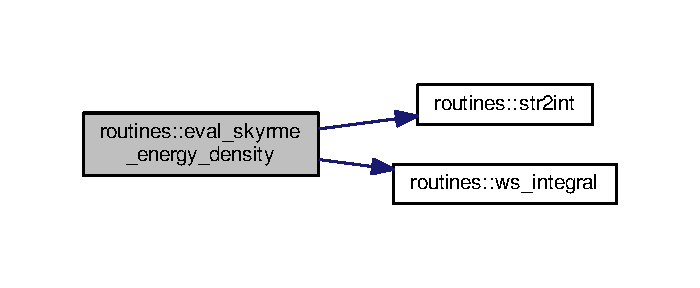
\includegraphics[width=336pt]{namespaceroutines_ae210968d134fbcc79297971cc4fefb82_cgraph}
\end{center}
\end{figure}
Here is the caller graph for this function\+:
\nopagebreak
\begin{figure}[H]
\begin{center}
\leavevmode
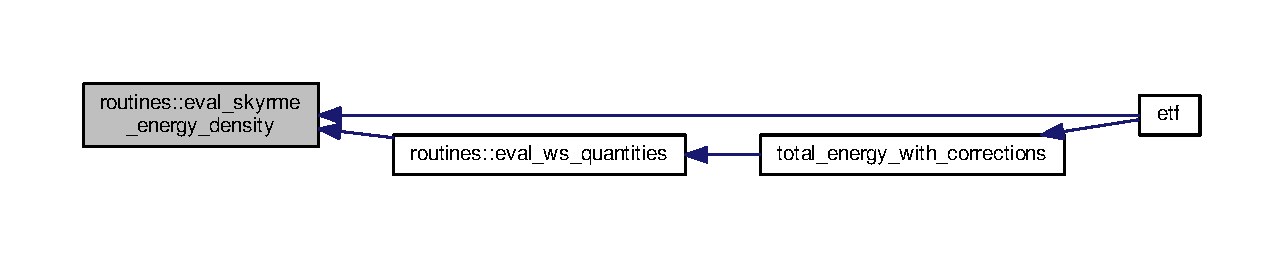
\includegraphics[width=350pt]{namespaceroutines_ae210968d134fbcc79297971cc4fefb82_icgraph}
\end{center}
\end{figure}
\mbox{\Hypertarget{namespaceroutines_a97bfcff7e603cf9df3dcd48ae21b4612}\label{namespaceroutines_a97bfcff7e603cf9df3dcd48ae21b4612}} 
\index{routines@{routines}!eval\+\_\+tau\+\_\+etf@{eval\+\_\+tau\+\_\+etf}}
\index{eval\+\_\+tau\+\_\+etf@{eval\+\_\+tau\+\_\+etf}!routines@{routines}}
\subsubsection{\texorpdfstring{eval\+\_\+tau\+\_\+etf()}{eval\_tau\_etf()}}
{\footnotesize\ttfamily subroutine routines\+::eval\+\_\+tau\+\_\+etf (\begin{DoxyParamCaption}{ }\end{DoxyParamCaption})}



Subroutine to calculate the kinetic energy density $\tau_{ETF}$ with the (extended) Thomas-\/\+Fermi approximation at order specified by \char`\"{}etf\+\_\+order\char`\"{}. 

\begin{DoxyAuthor}{Author}
M. Shelley 
\end{DoxyAuthor}
Here is the call graph for this function\+:
\nopagebreak
\begin{figure}[H]
\begin{center}
\leavevmode
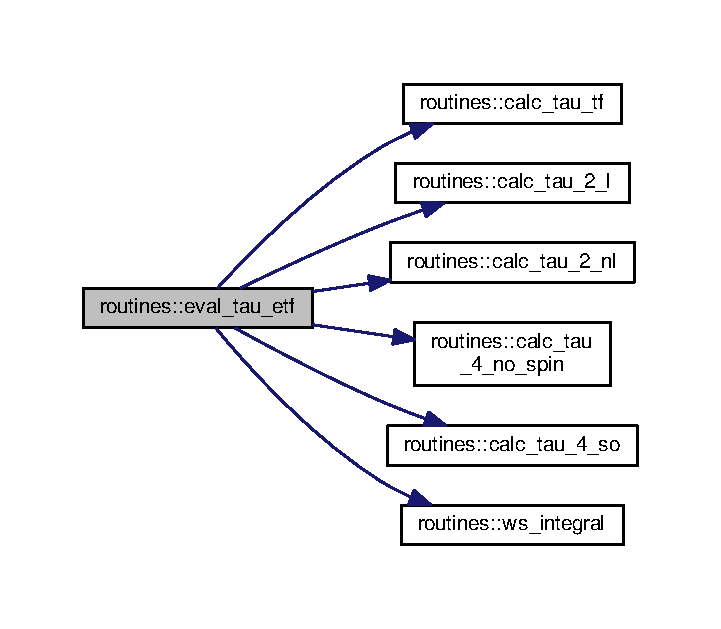
\includegraphics[width=346pt]{namespaceroutines_a97bfcff7e603cf9df3dcd48ae21b4612_cgraph}
\end{center}
\end{figure}
Here is the caller graph for this function\+:
\nopagebreak
\begin{figure}[H]
\begin{center}
\leavevmode
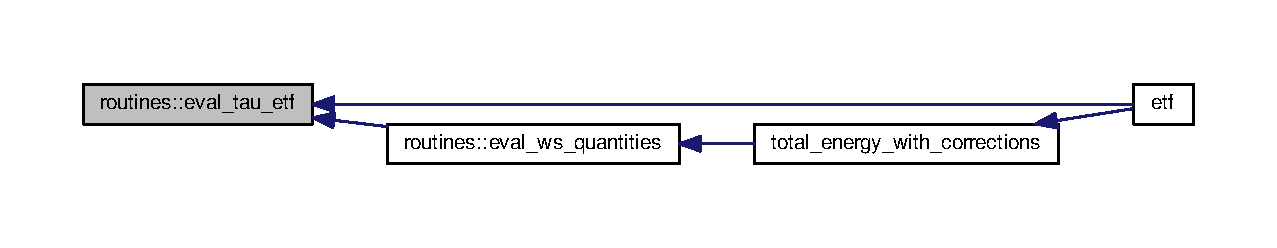
\includegraphics[width=350pt]{namespaceroutines_a97bfcff7e603cf9df3dcd48ae21b4612_icgraph}
\end{center}
\end{figure}
\mbox{\Hypertarget{namespaceroutines_a6ee5e5cd7ce81b013d18b19f5f9a4092}\label{namespaceroutines_a6ee5e5cd7ce81b013d18b19f5f9a4092}} 
\index{routines@{routines}!eval\+\_\+u\+\_\+q@{eval\+\_\+u\+\_\+q}}
\index{eval\+\_\+u\+\_\+q@{eval\+\_\+u\+\_\+q}!routines@{routines}}
\subsubsection{\texorpdfstring{eval\+\_\+u\+\_\+q()}{eval\_u\_q()}}
{\footnotesize\ttfamily subroutine routines\+::eval\+\_\+u\+\_\+q (\begin{DoxyParamCaption}{ }\end{DoxyParamCaption})}



Subroutine to evaluate the central fields $U_q$. 

\begin{DoxyAuthor}{Author}
M. Shelley 
\end{DoxyAuthor}
Here is the call graph for this function\+:
\nopagebreak
\begin{figure}[H]
\begin{center}
\leavevmode
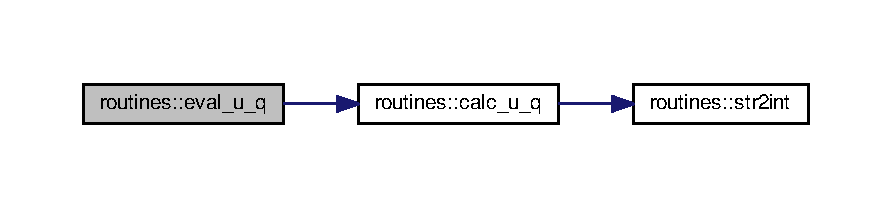
\includegraphics[width=350pt]{namespaceroutines_a6ee5e5cd7ce81b013d18b19f5f9a4092_cgraph}
\end{center}
\end{figure}
Here is the caller graph for this function\+:
\nopagebreak
\begin{figure}[H]
\begin{center}
\leavevmode
\includegraphics[width=350pt]{namespaceroutines_a6ee5e5cd7ce81b013d18b19f5f9a4092_icgraph}
\end{center}
\end{figure}
\mbox{\Hypertarget{namespaceroutines_a93de76f3b26ead66893f46dc4892dbcb}\label{namespaceroutines_a93de76f3b26ead66893f46dc4892dbcb}} 
\index{routines@{routines}!eval\+\_\+ws\+\_\+quantities@{eval\+\_\+ws\+\_\+quantities}}
\index{eval\+\_\+ws\+\_\+quantities@{eval\+\_\+ws\+\_\+quantities}!routines@{routines}}
\subsubsection{\texorpdfstring{eval\+\_\+ws\+\_\+quantities()}{eval\_ws\_quantities()}}
{\footnotesize\ttfamily subroutine routines\+::eval\+\_\+ws\+\_\+quantities (\begin{DoxyParamCaption}{ }\end{DoxyParamCaption})}



Subroutine to evaluate the various densities, fields, derivatives, energies, and particle numbers in the WS cell with densities $rho_q$. 

\begin{DoxyAuthor}{Author}
M. Shelley 
\end{DoxyAuthor}
Here is the call graph for this function\+:
\nopagebreak
\begin{figure}[H]
\begin{center}
\leavevmode
\includegraphics[width=350pt]{namespaceroutines_a93de76f3b26ead66893f46dc4892dbcb_cgraph}
\end{center}
\end{figure}
Here is the caller graph for this function\+:
\nopagebreak
\begin{figure}[H]
\begin{center}
\leavevmode
\includegraphics[width=350pt]{namespaceroutines_a93de76f3b26ead66893f46dc4892dbcb_icgraph}
\end{center}
\end{figure}
\mbox{\Hypertarget{namespaceroutines_af143340288720f8019e944ec7110a84e}\label{namespaceroutines_af143340288720f8019e944ec7110a84e}} 
\index{routines@{routines}!extrapolate\+\_\+back\+\_\+3@{extrapolate\+\_\+back\+\_\+3}}
\index{extrapolate\+\_\+back\+\_\+3@{extrapolate\+\_\+back\+\_\+3}!routines@{routines}}
\subsubsection{\texorpdfstring{extrapolate\+\_\+back\+\_\+3()}{extrapolate\_back\_3()}}
{\footnotesize\ttfamily subroutine routines\+::extrapolate\+\_\+back\+\_\+3 (\begin{DoxyParamCaption}\item[{real(kind=dp), dimension(\+:), intent(inout)}]{grid }\end{DoxyParamCaption})}



Subroutine to extrapolate back 3 points on the r mesh, to faciliate the calculation of first and second derivatives using a 5-\/point stencil. Values in grid start at 4, extrapolated values are put in elements 3,2,1. Coefficients come from solving 4th-\/order polynomial, assuming that f\textquotesingle{}(0) = 0, and f(-\/h) = f(h). 

\begin{DoxyAuthor}{Author}
M. Shelley 
\end{DoxyAuthor}

\begin{DoxyParams}[1]{Parameters}
\mbox{\tt in,out}  & {\em grid} & Array of quantity evaluated on r mesh, with 3 elements before r = dr \\
\hline
\end{DoxyParams}
Here is the caller graph for this function\+:
\nopagebreak
\begin{figure}[H]
\begin{center}
\leavevmode
\includegraphics[width=350pt]{namespaceroutines_af143340288720f8019e944ec7110a84e_icgraph}
\end{center}
\end{figure}
\mbox{\Hypertarget{namespaceroutines_a5caa9b33bdf3c960b6bb3bfa96771181}\label{namespaceroutines_a5caa9b33bdf3c960b6bb3bfa96771181}} 
\index{routines@{routines}!initialise\+\_\+uniform\+\_\+mesh@{initialise\+\_\+uniform\+\_\+mesh}}
\index{initialise\+\_\+uniform\+\_\+mesh@{initialise\+\_\+uniform\+\_\+mesh}!routines@{routines}}
\subsubsection{\texorpdfstring{initialise\+\_\+uniform\+\_\+mesh()}{initialise\_uniform\_mesh()}}
{\footnotesize\ttfamily subroutine routines\+::initialise\+\_\+uniform\+\_\+mesh (\begin{DoxyParamCaption}{ }\end{DoxyParamCaption})}



Subroutine to calculate number of mesh points for a uniform grid, allocate array for r, and then populate r with the mesh points. 

\begin{DoxyAuthor}{Author}
M. Shelley 
\end{DoxyAuthor}
Here is the caller graph for this function\+:
\nopagebreak
\begin{figure}[H]
\begin{center}
\leavevmode
\includegraphics[width=237pt]{namespaceroutines_a5caa9b33bdf3c960b6bb3bfa96771181_icgraph}
\end{center}
\end{figure}
\mbox{\Hypertarget{namespaceroutines_a635a2461a6c20207dd3b268842381ce3}\label{namespaceroutines_a635a2461a6c20207dd3b268842381ce3}} 
\index{routines@{routines}!lap\+\_\+sphe\+\_\+symm@{lap\+\_\+sphe\+\_\+symm}}
\index{lap\+\_\+sphe\+\_\+symm@{lap\+\_\+sphe\+\_\+symm}!routines@{routines}}
\subsubsection{\texorpdfstring{lap\+\_\+sphe\+\_\+symm()}{lap\_sphe\_symm()}}
{\footnotesize\ttfamily subroutine routines\+::lap\+\_\+sphe\+\_\+symm (\begin{DoxyParamCaption}\item[{real(kind=dp), dimension(-\/2\+:n), intent(in)}]{f,  }\item[{real(kind=dp), dimension(1\+:n), intent(in)}]{df\+\_\+dr,  }\item[{real(kind=dp), dimension(1\+:n), intent(inout)}]{d2f\+\_\+dr2 }\end{DoxyParamCaption})}



Subroutine to carry out Laplacian in spherical symmetry. 

\begin{DoxyAuthor}{Author}
M. Shelley 
\end{DoxyAuthor}

\begin{DoxyParams}[1]{Parameters}
\mbox{\tt in}  & {\em f} & Input function (1\+:n) with extrapolated values in -\/2,-\/1,0 \\
\hline
\mbox{\tt in}  & {\em df\+\_\+dr} & First derivative array \\
\hline
\mbox{\tt in,out}  & {\em d2f\+\_\+dr2} & Array for Laplacian \\
\hline
\end{DoxyParams}
Here is the call graph for this function\+:
\nopagebreak
\begin{figure}[H]
\begin{center}
\leavevmode
\includegraphics[width=312pt]{namespaceroutines_a635a2461a6c20207dd3b268842381ce3_cgraph}
\end{center}
\end{figure}
Here is the caller graph for this function\+:
\nopagebreak
\begin{figure}[H]
\begin{center}
\leavevmode
\includegraphics[width=350pt]{namespaceroutines_a635a2461a6c20207dd3b268842381ce3_icgraph}
\end{center}
\end{figure}
\mbox{\Hypertarget{namespaceroutines_a383e2bf5a1fa37fbf95dd5f6ddbcc6be}\label{namespaceroutines_a383e2bf5a1fa37fbf95dd5f6ddbcc6be}} 
\index{routines@{routines}!pressure@{pressure}}
\index{pressure@{pressure}!routines@{routines}}
\subsubsection{\texorpdfstring{pressure()}{pressure()}}
{\footnotesize\ttfamily subroutine routines\+::pressure (\begin{DoxyParamCaption}{ }\end{DoxyParamCaption})}



Subroutine to calculate the nuclear contribution to the pressure, and then the total pressure. 

\begin{DoxyAuthor}{Author}
M. Shelley 
\end{DoxyAuthor}
Here is the call graph for this function\+:
\nopagebreak
\begin{figure}[H]
\begin{center}
\leavevmode
\includegraphics[width=295pt]{namespaceroutines_a383e2bf5a1fa37fbf95dd5f6ddbcc6be_cgraph}
\end{center}
\end{figure}
Here is the caller graph for this function\+:
\nopagebreak
\begin{figure}[H]
\begin{center}
\leavevmode
\includegraphics[width=350pt]{namespaceroutines_a383e2bf5a1fa37fbf95dd5f6ddbcc6be_icgraph}
\end{center}
\end{figure}
\mbox{\Hypertarget{namespaceroutines_a8146fb4359e556bad19f882b8aabfc4b}\label{namespaceroutines_a8146fb4359e556bad19f882b8aabfc4b}} 
\index{routines@{routines}!str2int@{str2int}}
\index{str2int@{str2int}!routines@{routines}}
\subsubsection{\texorpdfstring{str2int()}{str2int()}}
{\footnotesize\ttfamily integer function routines\+::str2int (\begin{DoxyParamCaption}\item[{character(len=$\ast$), intent(in)}]{string }\end{DoxyParamCaption})}

Here is the caller graph for this function\+:
\nopagebreak
\begin{figure}[H]
\begin{center}
\leavevmode
\includegraphics[width=350pt]{namespaceroutines_a8146fb4359e556bad19f882b8aabfc4b_icgraph}
\end{center}
\end{figure}
\mbox{\Hypertarget{namespaceroutines_a81e61269fb96b5478fd7140a1f185ec1}\label{namespaceroutines_a81e61269fb96b5478fd7140a1f185ec1}} 
\index{routines@{routines}!write\+\_\+densities@{write\+\_\+densities}}
\index{write\+\_\+densities@{write\+\_\+densities}!routines@{routines}}
\subsubsection{\texorpdfstring{write\+\_\+densities()}{write\_densities()}}
{\footnotesize\ttfamily subroutine routines\+::write\+\_\+densities (\begin{DoxyParamCaption}{ }\end{DoxyParamCaption})}



Subroutine to write neutron and proton densities to files. 

\begin{DoxyAuthor}{Author}
M. Shelley 
\end{DoxyAuthor}
Here is the caller graph for this function\+:
\nopagebreak
\begin{figure}[H]
\begin{center}
\leavevmode
\includegraphics[width=350pt]{namespaceroutines_a81e61269fb96b5478fd7140a1f185ec1_icgraph}
\end{center}
\end{figure}
\mbox{\Hypertarget{namespaceroutines_a4a59953c814b7fa48f2c4bf31d1763a2}\label{namespaceroutines_a4a59953c814b7fa48f2c4bf31d1763a2}} 
\index{routines@{routines}!write\+\_\+fields@{write\+\_\+fields}}
\index{write\+\_\+fields@{write\+\_\+fields}!routines@{routines}}
\subsubsection{\texorpdfstring{write\+\_\+fields()}{write\_fields()}}
{\footnotesize\ttfamily subroutine routines\+::write\+\_\+fields (\begin{DoxyParamCaption}{ }\end{DoxyParamCaption})}



Subroutine to write neutron and proton fields to files. 

\begin{DoxyAuthor}{Author}
M. Shelley 
\end{DoxyAuthor}
Here is the caller graph for this function\+:
\nopagebreak
\begin{figure}[H]
\begin{center}
\leavevmode
\includegraphics[width=350pt]{namespaceroutines_a4a59953c814b7fa48f2c4bf31d1763a2_icgraph}
\end{center}
\end{figure}
\mbox{\Hypertarget{namespaceroutines_ad51ac6c5da6056a5346d7b15b3fbe7b4}\label{namespaceroutines_ad51ac6c5da6056a5346d7b15b3fbe7b4}} 
\index{routines@{routines}!write\+\_\+sp\+\_\+states\+\_\+p@{write\+\_\+sp\+\_\+states\+\_\+p}}
\index{write\+\_\+sp\+\_\+states\+\_\+p@{write\+\_\+sp\+\_\+states\+\_\+p}!routines@{routines}}
\subsubsection{\texorpdfstring{write\+\_\+sp\+\_\+states\+\_\+p()}{write\_sp\_states\_p()}}
{\footnotesize\ttfamily subroutine routines\+::write\+\_\+sp\+\_\+states\+\_\+p (\begin{DoxyParamCaption}{ }\end{DoxyParamCaption})}



Subroutine to write proton single particle energies to file, and extra details if B\+CS has been performed. 

\begin{DoxyAuthor}{Author}
M. Shelley 
\end{DoxyAuthor}
Here is the caller graph for this function\+:
\nopagebreak
\begin{figure}[H]
\begin{center}
\leavevmode
\includegraphics[width=350pt]{namespaceroutines_ad51ac6c5da6056a5346d7b15b3fbe7b4_icgraph}
\end{center}
\end{figure}
\mbox{\Hypertarget{namespaceroutines_a5737b4327dcaa959a9ee519e4fca42e8}\label{namespaceroutines_a5737b4327dcaa959a9ee519e4fca42e8}} 
\index{routines@{routines}!ws\+\_\+integral@{ws\+\_\+integral}}
\index{ws\+\_\+integral@{ws\+\_\+integral}!routines@{routines}}
\subsubsection{\texorpdfstring{ws\+\_\+integral()}{ws\_integral()}}
{\footnotesize\ttfamily real(kind=dp) function routines\+::ws\+\_\+integral (\begin{DoxyParamCaption}\item[{real(kind=dp), dimension(\+:), intent(in)}]{quantity,  }\item[{integer, intent(in)}]{n\+\_\+max }\end{DoxyParamCaption})}



Function to integrate a density or field over the whole W-\/S cell, using Simpson\textquotesingle{}s rule (+ Simpson\textquotesingle{}s 3/8 rule if odd number of points) 

\begin{DoxyAuthor}{Author}
M. Shelley 
\end{DoxyAuthor}

\begin{DoxyParams}[1]{Parameters}
\mbox{\tt in}  & {\em quantity} & Array of quantity, evaluated on r mesh, to be integrated \\
\hline
\mbox{\tt in}  & {\em n\+\_\+max} & Maximum mesh point in array for integration \\
\hline
\end{DoxyParams}
Here is the caller graph for this function\+:
\nopagebreak
\begin{figure}[H]
\begin{center}
\leavevmode
\includegraphics[width=350pt]{namespaceroutines_a5737b4327dcaa959a9ee519e4fca42e8_icgraph}
\end{center}
\end{figure}


\subsection{Variable Documentation}
\mbox{\Hypertarget{namespaceroutines_a4433ed4e6fbf0c81f38d8df1749be025}\label{namespaceroutines_a4433ed4e6fbf0c81f38d8df1749be025}} 
\index{routines@{routines}!file\+\_\+unit\+\_\+0@{file\+\_\+unit\+\_\+0}}
\index{file\+\_\+unit\+\_\+0@{file\+\_\+unit\+\_\+0}!routines@{routines}}
\subsubsection{\texorpdfstring{file\+\_\+unit\+\_\+0}{file\_unit\_0}}
{\footnotesize\ttfamily integer routines\+::file\+\_\+unit\+\_\+0}

\mbox{\Hypertarget{namespaceroutines_a806b34a65a0678e540be124100a0f908}\label{namespaceroutines_a806b34a65a0678e540be124100a0f908}} 
\index{routines@{routines}!file\+\_\+unit\+\_\+1@{file\+\_\+unit\+\_\+1}}
\index{file\+\_\+unit\+\_\+1@{file\+\_\+unit\+\_\+1}!routines@{routines}}
\subsubsection{\texorpdfstring{file\+\_\+unit\+\_\+1}{file\_unit\_1}}
{\footnotesize\ttfamily integer routines\+::file\+\_\+unit\+\_\+1}



Unit numbers for opening files. 


\hypertarget{namespacerspace}{}\section{rspace Module Reference}
\label{namespacerspace}\index{rspace@{rspace}}


Module to hold routines for calculating single particle energies. Written by A. Pastore, some variables and use statements modified by M. Shelley for integration into etf code.  


\subsection*{Functions/\+Subroutines}
\begin{DoxyCompactItemize}
\item 
subroutine \mbox{\hyperlink{namespacerspace_af32fb6df1b49e330db5a70e2b05faa5b}{boundary}} (h, Lmax, Ecut, Nmaxt, PS, N\+N\+ST, J\+JP, LP, EP, isospin)
\item 
subroutine \mbox{\hyperlink{namespacerspace_a95f8e6b75776b923eb4ab9cc71a3be33}{numerov}} (h, Nrmax, Emax0, N, L, J, E\+F\+I\+N\+AL, U, V, V\+SO, H\+ME, GI, G\+Iprimo, no)
\end{DoxyCompactItemize}


\subsection{Detailed Description}
Module to hold routines for calculating single particle energies. Written by A. Pastore, some variables and use statements modified by M. Shelley for integration into etf code. 

\begin{DoxyAuthor}{Author}
A. Pastore, M. Shelley 
\end{DoxyAuthor}


\subsection{Function/\+Subroutine Documentation}
\mbox{\Hypertarget{namespacerspace_af32fb6df1b49e330db5a70e2b05faa5b}\label{namespacerspace_af32fb6df1b49e330db5a70e2b05faa5b}} 
\index{rspace@{rspace}!boundary@{boundary}}
\index{boundary@{boundary}!rspace@{rspace}}
\subsubsection{\texorpdfstring{boundary()}{boundary()}}
{\footnotesize\ttfamily subroutine rspace\+::boundary (\begin{DoxyParamCaption}\item[{double precision}]{h,  }\item[{integer}]{Lmax,  }\item[{double precision}]{Ecut,  }\item[{integer}]{Nmaxt,  }\item[{double precision, dimension(nmaxstate,nmaxt)}]{PS,  }\item[{integer}]{N\+N\+ST,  }\item[{integer, dimension(nmaxstate)}]{J\+JP,  }\item[{integer, dimension(nmaxstate)}]{LP,  }\item[{double precision, dimension(nmaxstate)}]{EP,  }\item[{integer}]{isospin }\end{DoxyParamCaption})}

Here is the call graph for this function\+:
\nopagebreak
\begin{figure}[H]
\begin{center}
\leavevmode
\includegraphics[width=297pt]{namespacerspace_af32fb6df1b49e330db5a70e2b05faa5b_cgraph}
\end{center}
\end{figure}
Here is the caller graph for this function\+:
\nopagebreak
\begin{figure}[H]
\begin{center}
\leavevmode
\includegraphics[width=350pt]{namespacerspace_af32fb6df1b49e330db5a70e2b05faa5b_icgraph}
\end{center}
\end{figure}
\mbox{\Hypertarget{namespacerspace_a95f8e6b75776b923eb4ab9cc71a3be33}\label{namespacerspace_a95f8e6b75776b923eb4ab9cc71a3be33}} 
\index{rspace@{rspace}!numerov@{numerov}}
\index{numerov@{numerov}!rspace@{rspace}}
\subsubsection{\texorpdfstring{numerov()}{numerov()}}
{\footnotesize\ttfamily subroutine rspace\+::numerov (\begin{DoxyParamCaption}\item[{double precision}]{h,  }\item[{integer}]{Nrmax,  }\item[{double precision}]{Emax0,  }\item[{integer}]{N,  }\item[{integer}]{L,  }\item[{integer}]{J,  }\item[{double precision}]{E\+F\+I\+N\+AL,  }\item[{double precision, dimension(nrmax)}]{U,  }\item[{double precision, dimension(nrmax)}]{V,  }\item[{double precision, dimension(nrmax)}]{V\+SO,  }\item[{double precision, dimension(nrmax)}]{H\+ME,  }\item[{double precision, dimension(nrmax)}]{GI,  }\item[{double precision, dimension(nrmax)}]{G\+Iprimo,  }\item[{integer}]{no }\end{DoxyParamCaption})}

Here is the caller graph for this function\+:
\nopagebreak
\begin{figure}[H]
\begin{center}
\leavevmode
\includegraphics[width=350pt]{namespacerspace_a95f8e6b75776b923eb4ab9cc71a3be33_icgraph}
\end{center}
\end{figure}

\hypertarget{namespacestrutinsky}{}\section{strutinsky Module Reference}
\label{namespacestrutinsky}\index{strutinsky@{strutinsky}}


Module to hold routines for carrying out Strutinsky correction.  


\subsection*{Functions/\+Subroutines}
\begin{DoxyCompactItemize}
\item 
subroutine \mbox{\hyperlink{namespacestrutinsky_a6eeba7570095328226f37df3e89b7a18}{sp\+\_\+states\+\_\+setup}} ()
\begin{DoxyCompactList}\small\item\em Subroutine to allocate + initialise variables needed in \textquotesingle{}boundary\textquotesingle{} routine, and allocate arrays needed for B\+CS. \end{DoxyCompactList}\item 
subroutine \mbox{\hyperlink{namespacestrutinsky_a0a07c6adfd14cbf345bf96b70d3f5d82}{sp\+\_\+states\+\_\+deallocate}} ()
\begin{DoxyCompactList}\small\item\em Subroutine to deallocate arrays needed in \textquotesingle{}boundary\textquotesingle{} routine, and deallocate arrays needed for B\+CS. \end{DoxyCompactList}\item 
subroutine \mbox{\hyperlink{namespacestrutinsky_a106e8ec285383b5042e8436a2376147a}{state\+\_\+sort}} (sp\+\_\+J, sp\+\_\+L, sp\+\_\+E, sp\+\_\+wfns)
\begin{DoxyCompactList}\small\item\em Subroutine to sort single particle states by their energies. Use bubble sort. \end{DoxyCompactList}\item 
subroutine \mbox{\hyperlink{namespacestrutinsky_a7a348b225e6556c53687ee28ee31b316}{calc\+\_\+e\+\_\+sc}} (q)
\begin{DoxyCompactList}\small\item\em Subroutine to calculate the Strutinsky shell correction energy for isospin $q$. First, sum over occupied states of s.\+p. energies. Second, integrate over W-\/S cell of smoothed E\+TF densities and fields. \end{DoxyCompactList}\item 
subroutine \mbox{\hyperlink{namespacestrutinsky_a2cc0d4130d68c345ffe3ffa73706e796}{calc\+\_\+e\+\_\+sc\+\_\+pair}} ()
\begin{DoxyCompactList}\small\item\em Subroutine to calculate the Strutinsky shell correction energy for protons, using B\+CS occupation probabilities. \end{DoxyCompactList}\end{DoxyCompactItemize}


\subsection{Detailed Description}
Module to hold routines for carrying out Strutinsky correction. 

\begin{DoxyAuthor}{Author}
M. Shelley 
\end{DoxyAuthor}


\subsection{Function/\+Subroutine Documentation}
\mbox{\Hypertarget{namespacestrutinsky_a7a348b225e6556c53687ee28ee31b316}\label{namespacestrutinsky_a7a348b225e6556c53687ee28ee31b316}} 
\index{strutinsky@{strutinsky}!calc\+\_\+e\+\_\+sc@{calc\+\_\+e\+\_\+sc}}
\index{calc\+\_\+e\+\_\+sc@{calc\+\_\+e\+\_\+sc}!strutinsky@{strutinsky}}
\subsubsection{\texorpdfstring{calc\+\_\+e\+\_\+sc()}{calc\_e\_sc()}}
{\footnotesize\ttfamily subroutine strutinsky\+::calc\+\_\+e\+\_\+sc (\begin{DoxyParamCaption}\item[{integer, intent(in)}]{q }\end{DoxyParamCaption})}



Subroutine to calculate the Strutinsky shell correction energy for isospin $q$. First, sum over occupied states of s.\+p. energies. Second, integrate over W-\/S cell of smoothed E\+TF densities and fields. 

\begin{DoxyAuthor}{Author}
M. Shelley 
\end{DoxyAuthor}

\begin{DoxyParams}[1]{Parameters}
\mbox{\tt in}  & {\em q} & Isospin\\
\hline
\mbox{\tt in}  & {\em q} & Isospin \\
\hline
\end{DoxyParams}
Here is the call graph for this function\+:
\nopagebreak
\begin{figure}[H]
\begin{center}
\leavevmode
\includegraphics[width=350pt]{namespacestrutinsky_a7a348b225e6556c53687ee28ee31b316_cgraph}
\end{center}
\end{figure}
Here is the caller graph for this function\+:
\nopagebreak
\begin{figure}[H]
\begin{center}
\leavevmode
\includegraphics[width=350pt]{namespacestrutinsky_a7a348b225e6556c53687ee28ee31b316_icgraph}
\end{center}
\end{figure}
\mbox{\Hypertarget{namespacestrutinsky_a2cc0d4130d68c345ffe3ffa73706e796}\label{namespacestrutinsky_a2cc0d4130d68c345ffe3ffa73706e796}} 
\index{strutinsky@{strutinsky}!calc\+\_\+e\+\_\+sc\+\_\+pair@{calc\+\_\+e\+\_\+sc\+\_\+pair}}
\index{calc\+\_\+e\+\_\+sc\+\_\+pair@{calc\+\_\+e\+\_\+sc\+\_\+pair}!strutinsky@{strutinsky}}
\subsubsection{\texorpdfstring{calc\+\_\+e\+\_\+sc\+\_\+pair()}{calc\_e\_sc\_pair()}}
{\footnotesize\ttfamily subroutine strutinsky\+::calc\+\_\+e\+\_\+sc\+\_\+pair (\begin{DoxyParamCaption}{ }\end{DoxyParamCaption})}



Subroutine to calculate the Strutinsky shell correction energy for protons, using B\+CS occupation probabilities. 

\begin{DoxyAuthor}{Author}
M. Shelley 
\end{DoxyAuthor}
Here is the call graph for this function\+:
\nopagebreak
\begin{figure}[H]
\begin{center}
\leavevmode
\includegraphics[width=317pt]{namespacestrutinsky_a2cc0d4130d68c345ffe3ffa73706e796_cgraph}
\end{center}
\end{figure}
Here is the caller graph for this function\+:
\nopagebreak
\begin{figure}[H]
\begin{center}
\leavevmode
\includegraphics[width=350pt]{namespacestrutinsky_a2cc0d4130d68c345ffe3ffa73706e796_icgraph}
\end{center}
\end{figure}
\mbox{\Hypertarget{namespacestrutinsky_a0a07c6adfd14cbf345bf96b70d3f5d82}\label{namespacestrutinsky_a0a07c6adfd14cbf345bf96b70d3f5d82}} 
\index{strutinsky@{strutinsky}!sp\+\_\+states\+\_\+deallocate@{sp\+\_\+states\+\_\+deallocate}}
\index{sp\+\_\+states\+\_\+deallocate@{sp\+\_\+states\+\_\+deallocate}!strutinsky@{strutinsky}}
\subsubsection{\texorpdfstring{sp\+\_\+states\+\_\+deallocate()}{sp\_states\_deallocate()}}
{\footnotesize\ttfamily subroutine strutinsky\+::sp\+\_\+states\+\_\+deallocate (\begin{DoxyParamCaption}{ }\end{DoxyParamCaption})}



Subroutine to deallocate arrays needed in \textquotesingle{}boundary\textquotesingle{} routine, and deallocate arrays needed for B\+CS. 

\begin{DoxyAuthor}{Author}
M. Shelley 
\end{DoxyAuthor}
Here is the caller graph for this function\+:
\nopagebreak
\begin{figure}[H]
\begin{center}
\leavevmode
\includegraphics[width=350pt]{namespacestrutinsky_a0a07c6adfd14cbf345bf96b70d3f5d82_icgraph}
\end{center}
\end{figure}
\mbox{\Hypertarget{namespacestrutinsky_a6eeba7570095328226f37df3e89b7a18}\label{namespacestrutinsky_a6eeba7570095328226f37df3e89b7a18}} 
\index{strutinsky@{strutinsky}!sp\+\_\+states\+\_\+setup@{sp\+\_\+states\+\_\+setup}}
\index{sp\+\_\+states\+\_\+setup@{sp\+\_\+states\+\_\+setup}!strutinsky@{strutinsky}}
\subsubsection{\texorpdfstring{sp\+\_\+states\+\_\+setup()}{sp\_states\_setup()}}
{\footnotesize\ttfamily subroutine strutinsky\+::sp\+\_\+states\+\_\+setup (\begin{DoxyParamCaption}{ }\end{DoxyParamCaption})}



Subroutine to allocate + initialise variables needed in \textquotesingle{}boundary\textquotesingle{} routine, and allocate arrays needed for B\+CS. 

\begin{DoxyAuthor}{Author}
M. Shelley 
\end{DoxyAuthor}
Here is the caller graph for this function\+:
\nopagebreak
\begin{figure}[H]
\begin{center}
\leavevmode
\includegraphics[width=350pt]{namespacestrutinsky_a6eeba7570095328226f37df3e89b7a18_icgraph}
\end{center}
\end{figure}
\mbox{\Hypertarget{namespacestrutinsky_a106e8ec285383b5042e8436a2376147a}\label{namespacestrutinsky_a106e8ec285383b5042e8436a2376147a}} 
\index{strutinsky@{strutinsky}!state\+\_\+sort@{state\+\_\+sort}}
\index{state\+\_\+sort@{state\+\_\+sort}!strutinsky@{strutinsky}}
\subsubsection{\texorpdfstring{state\+\_\+sort()}{state\_sort()}}
{\footnotesize\ttfamily subroutine strutinsky\+::state\+\_\+sort (\begin{DoxyParamCaption}\item[{integer, dimension(\+:), intent(inout)}]{sp\+\_\+J,  }\item[{integer, dimension(\+:), intent(inout)}]{sp\+\_\+L,  }\item[{real(kind=dp), dimension(\+:), intent(inout)}]{sp\+\_\+E,  }\item[{real(kind=dp), dimension(\+:,\+:), intent(inout)}]{sp\+\_\+wfns }\end{DoxyParamCaption})}



Subroutine to sort single particle states by their energies. Use bubble sort. 

\begin{DoxyAuthor}{Author}
M. Shelley 
\end{DoxyAuthor}

\begin{DoxyParams}[1]{Parameters}
\mbox{\tt in,out}  & {\em sp\+\_\+J} & Array for (2)J\textquotesingle{}s of single particle states \\
\hline
\mbox{\tt in,out}  & {\em sp\+\_\+L} & Array for L\textquotesingle{}s of single particle states \\
\hline
\mbox{\tt in,out}  & {\em sp\+\_\+E} & Array for energies of single particle states \\
\hline
\mbox{\tt in,out}  & {\em sp\+\_\+wfns} & Array for wavefunctions of single particle states \\
\hline
\end{DoxyParams}
Here is the caller graph for this function\+:
\nopagebreak
\begin{figure}[H]
\begin{center}
\leavevmode
\includegraphics[width=350pt]{namespacestrutinsky_a106e8ec285383b5042e8436a2376147a_icgraph}
\end{center}
\end{figure}

\hypertarget{namespacetest}{}\section{test Module Reference}
\label{namespacetest}\index{test@{test}}


Module to hold test routines.  


\subsection*{Functions/\+Subroutines}
\begin{DoxyCompactItemize}
\item 
subroutine \mbox{\hyperlink{namespacetest_a2d72f655d80bac0b01030b9cbda3518f}{read\+\_\+test\+\_\+params}} ()
\begin{DoxyCompactList}\small\item\em Subroutine to read from \char`\"{}test\+\_\+input.\+in\char`\"{} parameters used for test routines. \end{DoxyCompactList}\item 
subroutine \mbox{\hyperlink{namespacetest_ac81b1d59a968470b8ef8a165101df52c}{test\+\_\+densities}} ()
\begin{DoxyCompactList}\small\item\em Subroutine to calculate the density profiles using sample parameters. \end{DoxyCompactList}\item 
subroutine \mbox{\hyperlink{namespacetest_a50469f436f9c4caa447dafc48e311558}{test\+\_\+density\+\_\+derivs}} ()
\begin{DoxyCompactList}\small\item\em Subroutine to test some derivatives of the total and individual densities. \end{DoxyCompactList}\item 
subroutine \mbox{\hyperlink{namespacetest_ac49b81619b874cdd8276af19d24675cc}{test\+\_\+eff\+\_\+mass}} ()
\begin{DoxyCompactList}\small\item\em Subroutine to test effective masses $fm^{-3}$. \end{DoxyCompactList}\item 
subroutine \mbox{\hyperlink{namespacetest_a377babe07d6ab6f0791233afee079582}{test\+\_\+kinetic\+\_\+densities}} ()
\begin{DoxyCompactList}\small\item\em Subroutine to test kinetic energy densities. \end{DoxyCompactList}\item 
subroutine \mbox{\hyperlink{namespacetest_a3e49a3b6fd835efb13dd446bfb6e8b1f}{test\+\_\+spin\+\_\+current\+\_\+densities}} ()
\begin{DoxyCompactList}\small\item\em Subroutine to write spin current densities and spin-\/orbit fields to file. \end{DoxyCompactList}\item 
subroutine \mbox{\hyperlink{namespacetest_a12069a39539c68f8d22f7eb4219d2e2b}{orders\+\_\+kinetic\+\_\+densities}} ()
\begin{DoxyCompactList}\small\item\em Subroutine to write order-\/by-\/order comparison of kinetic densities to file. \end{DoxyCompactList}\item 
subroutine \mbox{\hyperlink{namespacetest_a5693dbb30b96995df35fa720f0ab1436}{test\+\_\+central\+\_\+potentials}} ()
\begin{DoxyCompactList}\small\item\em Subroutine to write spin central potentials to file. \end{DoxyCompactList}\item 
subroutine \mbox{\hyperlink{namespacetest_ae6399ba2e0d2b484e6b467b2cee74a1b}{write\+\_\+ws\+\_\+cell\+\_\+array\+\_\+quantity}} (quantity)
\begin{DoxyCompactList}\small\item\em Utility subroutine that can be called anywhere at any time, for writing a quantity (evaluated over WS cell) to file. \end{DoxyCompactList}\item 
subroutine \mbox{\hyperlink{namespacetest_af860540d68e055817e3f618b7a04298a}{test\+\_\+calc\+\_\+particle\+\_\+number}} ()
\begin{DoxyCompactList}\small\item\em Subroutine to test calculation of neutron and proton particle numbers. \end{DoxyCompactList}\item 
subroutine \mbox{\hyperlink{namespacetest_ae4857dad0359d5f90718d5593398f8b3}{test\+\_\+calc\+\_\+coulomb\+\_\+energy}} ()
\begin{DoxyCompactList}\small\item\em Subroutine to test calculation of Coulomb energy. \end{DoxyCompactList}\item 
subroutine \mbox{\hyperlink{namespacetest_aa2a14f70fb7372abc970b6271f19417f}{test\+\_\+calc\+\_\+skyrme\+\_\+energy}} ()
\begin{DoxyCompactList}\small\item\em Subroutine to test calculation of Skyrme energy. \end{DoxyCompactList}\item 
subroutine \mbox{\hyperlink{namespacetest_abeb5e336395994821e96838b809e4140}{test\+\_\+sp\+\_\+energies}} ()
\begin{DoxyCompactList}\small\item\em Subroutine to test calculation of single particle energies. \end{DoxyCompactList}\item 
subroutine \mbox{\hyperlink{namespacetest_afde013e321ba30ada173fc343ca1fa6d}{test\+\_\+si\+\_\+correction}} ()
\begin{DoxyCompactList}\small\item\em Subroutine to test the Strutinsky integral correction. \end{DoxyCompactList}\item 
subroutine \mbox{\hyperlink{namespacetest_a8eb520f312c2647e714f169e9d5b8421}{bartel\+\_\+bencheikh\+\_\+benchmark}} ()
\begin{DoxyCompactList}\small\item\em Subroutine to check different contributions to $\tau_{ETF}$ at 2nd order, for comparison with results in Bartel and Bencheikh (2002) \end{DoxyCompactList}\end{DoxyCompactItemize}
\subsection*{Variables}
\begin{DoxyCompactItemize}
\item 
integer \mbox{\hyperlink{namespacetest_a91c93b5bfe044cfbaabf6b3acfe3be00}{file\+\_\+unit}}
\item 
integer \mbox{\hyperlink{namespacetest_aed47eec898fde16ebc3dae8f3c61abef}{file\+\_\+unit\+\_\+2}}
\begin{DoxyCompactList}\small\item\em Unit numbers for opening files. \end{DoxyCompactList}\item 
integer \mbox{\hyperlink{namespacetest_ab8cdf368336f888e9382efe275ce4d16}{sample\+\_\+profile}}
\begin{DoxyCompactList}\small\item\em Test density profile to use. \end{DoxyCompactList}\end{DoxyCompactItemize}


\subsection{Detailed Description}
Module to hold test routines. 

\begin{DoxyAuthor}{Author}
M. Shelley 
\end{DoxyAuthor}


\subsection{Function/\+Subroutine Documentation}
\mbox{\Hypertarget{namespacetest_a8eb520f312c2647e714f169e9d5b8421}\label{namespacetest_a8eb520f312c2647e714f169e9d5b8421}} 
\index{test@{test}!bartel\+\_\+bencheikh\+\_\+benchmark@{bartel\+\_\+bencheikh\+\_\+benchmark}}
\index{bartel\+\_\+bencheikh\+\_\+benchmark@{bartel\+\_\+bencheikh\+\_\+benchmark}!test@{test}}
\subsubsection{\texorpdfstring{bartel\+\_\+bencheikh\+\_\+benchmark()}{bartel\_bencheikh\_benchmark()}}
{\footnotesize\ttfamily subroutine test\+::bartel\+\_\+bencheikh\+\_\+benchmark (\begin{DoxyParamCaption}{ }\end{DoxyParamCaption})}



Subroutine to check different contributions to $\tau_{ETF}$ at 2nd order, for comparison with results in Bartel and Bencheikh (2002) 

\begin{DoxyAuthor}{Author}
M. Shelley 
\end{DoxyAuthor}
Here is the caller graph for this function\+:
\nopagebreak
\begin{figure}[H]
\begin{center}
\leavevmode
\includegraphics[width=258pt]{namespacetest_a8eb520f312c2647e714f169e9d5b8421_icgraph}
\end{center}
\end{figure}
\mbox{\Hypertarget{namespacetest_a12069a39539c68f8d22f7eb4219d2e2b}\label{namespacetest_a12069a39539c68f8d22f7eb4219d2e2b}} 
\index{test@{test}!orders\+\_\+kinetic\+\_\+densities@{orders\+\_\+kinetic\+\_\+densities}}
\index{orders\+\_\+kinetic\+\_\+densities@{orders\+\_\+kinetic\+\_\+densities}!test@{test}}
\subsubsection{\texorpdfstring{orders\+\_\+kinetic\+\_\+densities()}{orders\_kinetic\_densities()}}
{\footnotesize\ttfamily subroutine test\+::orders\+\_\+kinetic\+\_\+densities (\begin{DoxyParamCaption}{ }\end{DoxyParamCaption})}



Subroutine to write order-\/by-\/order comparison of kinetic densities to file. 

\begin{DoxyAuthor}{Author}
M. Shelley 
\end{DoxyAuthor}
Here is the caller graph for this function\+:
\nopagebreak
\begin{figure}[H]
\begin{center}
\leavevmode
\includegraphics[width=245pt]{namespacetest_a12069a39539c68f8d22f7eb4219d2e2b_icgraph}
\end{center}
\end{figure}
\mbox{\Hypertarget{namespacetest_a2d72f655d80bac0b01030b9cbda3518f}\label{namespacetest_a2d72f655d80bac0b01030b9cbda3518f}} 
\index{test@{test}!read\+\_\+test\+\_\+params@{read\+\_\+test\+\_\+params}}
\index{read\+\_\+test\+\_\+params@{read\+\_\+test\+\_\+params}!test@{test}}
\subsubsection{\texorpdfstring{read\+\_\+test\+\_\+params()}{read\_test\_params()}}
{\footnotesize\ttfamily subroutine test\+::read\+\_\+test\+\_\+params (\begin{DoxyParamCaption}{ }\end{DoxyParamCaption})}



Subroutine to read from \char`\"{}test\+\_\+input.\+in\char`\"{} parameters used for test routines. 

\begin{DoxyAuthor}{Author}
M. Shelley 
\end{DoxyAuthor}
Here is the caller graph for this function\+:
\nopagebreak
\begin{figure}[H]
\begin{center}
\leavevmode
\includegraphics[width=262pt]{namespacetest_a2d72f655d80bac0b01030b9cbda3518f_icgraph}
\end{center}
\end{figure}
\mbox{\Hypertarget{namespacetest_ae4857dad0359d5f90718d5593398f8b3}\label{namespacetest_ae4857dad0359d5f90718d5593398f8b3}} 
\index{test@{test}!test\+\_\+calc\+\_\+coulomb\+\_\+energy@{test\+\_\+calc\+\_\+coulomb\+\_\+energy}}
\index{test\+\_\+calc\+\_\+coulomb\+\_\+energy@{test\+\_\+calc\+\_\+coulomb\+\_\+energy}!test@{test}}
\subsubsection{\texorpdfstring{test\+\_\+calc\+\_\+coulomb\+\_\+energy()}{test\_calc\_coulomb\_energy()}}
{\footnotesize\ttfamily subroutine test\+::test\+\_\+calc\+\_\+coulomb\+\_\+energy (\begin{DoxyParamCaption}{ }\end{DoxyParamCaption})}



Subroutine to test calculation of Coulomb energy. 

\begin{DoxyAuthor}{Author}
M. Shelley 
\end{DoxyAuthor}
Here is the caller graph for this function\+:
\nopagebreak
\begin{figure}[H]
\begin{center}
\leavevmode
\includegraphics[width=266pt]{namespacetest_ae4857dad0359d5f90718d5593398f8b3_icgraph}
\end{center}
\end{figure}
\mbox{\Hypertarget{namespacetest_af860540d68e055817e3f618b7a04298a}\label{namespacetest_af860540d68e055817e3f618b7a04298a}} 
\index{test@{test}!test\+\_\+calc\+\_\+particle\+\_\+number@{test\+\_\+calc\+\_\+particle\+\_\+number}}
\index{test\+\_\+calc\+\_\+particle\+\_\+number@{test\+\_\+calc\+\_\+particle\+\_\+number}!test@{test}}
\subsubsection{\texorpdfstring{test\+\_\+calc\+\_\+particle\+\_\+number()}{test\_calc\_particle\_number()}}
{\footnotesize\ttfamily subroutine test\+::test\+\_\+calc\+\_\+particle\+\_\+number (\begin{DoxyParamCaption}{ }\end{DoxyParamCaption})}



Subroutine to test calculation of neutron and proton particle numbers. 

\begin{DoxyAuthor}{Author}
M. Shelley 
\end{DoxyAuthor}
Here is the caller graph for this function\+:
\nopagebreak
\begin{figure}[H]
\begin{center}
\leavevmode
\includegraphics[width=261pt]{namespacetest_af860540d68e055817e3f618b7a04298a_icgraph}
\end{center}
\end{figure}
\mbox{\Hypertarget{namespacetest_aa2a14f70fb7372abc970b6271f19417f}\label{namespacetest_aa2a14f70fb7372abc970b6271f19417f}} 
\index{test@{test}!test\+\_\+calc\+\_\+skyrme\+\_\+energy@{test\+\_\+calc\+\_\+skyrme\+\_\+energy}}
\index{test\+\_\+calc\+\_\+skyrme\+\_\+energy@{test\+\_\+calc\+\_\+skyrme\+\_\+energy}!test@{test}}
\subsubsection{\texorpdfstring{test\+\_\+calc\+\_\+skyrme\+\_\+energy()}{test\_calc\_skyrme\_energy()}}
{\footnotesize\ttfamily subroutine test\+::test\+\_\+calc\+\_\+skyrme\+\_\+energy (\begin{DoxyParamCaption}{ }\end{DoxyParamCaption})}



Subroutine to test calculation of Skyrme energy. 

\begin{DoxyAuthor}{Author}
M. Shelley 
\end{DoxyAuthor}
Here is the caller graph for this function\+:
\nopagebreak
\begin{figure}[H]
\begin{center}
\leavevmode
\includegraphics[width=261pt]{namespacetest_aa2a14f70fb7372abc970b6271f19417f_icgraph}
\end{center}
\end{figure}
\mbox{\Hypertarget{namespacetest_a5693dbb30b96995df35fa720f0ab1436}\label{namespacetest_a5693dbb30b96995df35fa720f0ab1436}} 
\index{test@{test}!test\+\_\+central\+\_\+potentials@{test\+\_\+central\+\_\+potentials}}
\index{test\+\_\+central\+\_\+potentials@{test\+\_\+central\+\_\+potentials}!test@{test}}
\subsubsection{\texorpdfstring{test\+\_\+central\+\_\+potentials()}{test\_central\_potentials()}}
{\footnotesize\ttfamily subroutine test\+::test\+\_\+central\+\_\+potentials (\begin{DoxyParamCaption}{ }\end{DoxyParamCaption})}



Subroutine to write spin central potentials to file. 

\begin{DoxyAuthor}{Author}
M. Shelley 
\end{DoxyAuthor}
Here is the caller graph for this function\+:
\nopagebreak
\begin{figure}[H]
\begin{center}
\leavevmode
\includegraphics[width=235pt]{namespacetest_a5693dbb30b96995df35fa720f0ab1436_icgraph}
\end{center}
\end{figure}
\mbox{\Hypertarget{namespacetest_ac81b1d59a968470b8ef8a165101df52c}\label{namespacetest_ac81b1d59a968470b8ef8a165101df52c}} 
\index{test@{test}!test\+\_\+densities@{test\+\_\+densities}}
\index{test\+\_\+densities@{test\+\_\+densities}!test@{test}}
\subsubsection{\texorpdfstring{test\+\_\+densities()}{test\_densities()}}
{\footnotesize\ttfamily subroutine test\+::test\+\_\+densities (\begin{DoxyParamCaption}{ }\end{DoxyParamCaption})}



Subroutine to calculate the density profiles using sample parameters. 

\begin{DoxyAuthor}{Author}
M. Shelley 
\end{DoxyAuthor}
Here is the call graph for this function\+:
\nopagebreak
\begin{figure}[H]
\begin{center}
\leavevmode
\includegraphics[width=320pt]{namespacetest_ac81b1d59a968470b8ef8a165101df52c_cgraph}
\end{center}
\end{figure}
Here is the caller graph for this function\+:
\nopagebreak
\begin{figure}[H]
\begin{center}
\leavevmode
\includegraphics[width=245pt]{namespacetest_ac81b1d59a968470b8ef8a165101df52c_icgraph}
\end{center}
\end{figure}
\mbox{\Hypertarget{namespacetest_a50469f436f9c4caa447dafc48e311558}\label{namespacetest_a50469f436f9c4caa447dafc48e311558}} 
\index{test@{test}!test\+\_\+density\+\_\+derivs@{test\+\_\+density\+\_\+derivs}}
\index{test\+\_\+density\+\_\+derivs@{test\+\_\+density\+\_\+derivs}!test@{test}}
\subsubsection{\texorpdfstring{test\+\_\+density\+\_\+derivs()}{test\_density\_derivs()}}
{\footnotesize\ttfamily subroutine test\+::test\+\_\+density\+\_\+derivs (\begin{DoxyParamCaption}{ }\end{DoxyParamCaption})}



Subroutine to test some derivatives of the total and individual densities. 

\begin{DoxyAuthor}{Author}
M. Shelley 
\end{DoxyAuthor}
Here is the caller graph for this function\+:
\nopagebreak
\begin{figure}[H]
\begin{center}
\leavevmode
\includegraphics[width=237pt]{namespacetest_a50469f436f9c4caa447dafc48e311558_icgraph}
\end{center}
\end{figure}
\mbox{\Hypertarget{namespacetest_ac49b81619b874cdd8276af19d24675cc}\label{namespacetest_ac49b81619b874cdd8276af19d24675cc}} 
\index{test@{test}!test\+\_\+eff\+\_\+mass@{test\+\_\+eff\+\_\+mass}}
\index{test\+\_\+eff\+\_\+mass@{test\+\_\+eff\+\_\+mass}!test@{test}}
\subsubsection{\texorpdfstring{test\+\_\+eff\+\_\+mass()}{test\_eff\_mass()}}
{\footnotesize\ttfamily subroutine test\+::test\+\_\+eff\+\_\+mass (\begin{DoxyParamCaption}{ }\end{DoxyParamCaption})}



Subroutine to test effective masses $fm^{-3}$. 

\begin{DoxyAuthor}{Author}
M. Shelley 
\end{DoxyAuthor}
Here is the caller graph for this function\+:
\nopagebreak
\begin{figure}[H]
\begin{center}
\leavevmode
\includegraphics[width=246pt]{namespacetest_ac49b81619b874cdd8276af19d24675cc_icgraph}
\end{center}
\end{figure}
\mbox{\Hypertarget{namespacetest_a377babe07d6ab6f0791233afee079582}\label{namespacetest_a377babe07d6ab6f0791233afee079582}} 
\index{test@{test}!test\+\_\+kinetic\+\_\+densities@{test\+\_\+kinetic\+\_\+densities}}
\index{test\+\_\+kinetic\+\_\+densities@{test\+\_\+kinetic\+\_\+densities}!test@{test}}
\subsubsection{\texorpdfstring{test\+\_\+kinetic\+\_\+densities()}{test\_kinetic\_densities()}}
{\footnotesize\ttfamily subroutine test\+::test\+\_\+kinetic\+\_\+densities (\begin{DoxyParamCaption}{ }\end{DoxyParamCaption})}



Subroutine to test kinetic energy densities. 

\begin{DoxyAuthor}{Author}
M. Shelley 
\end{DoxyAuthor}
Here is the caller graph for this function\+:
\nopagebreak
\begin{figure}[H]
\begin{center}
\leavevmode
\includegraphics[width=234pt]{namespacetest_a377babe07d6ab6f0791233afee079582_icgraph}
\end{center}
\end{figure}
\mbox{\Hypertarget{namespacetest_afde013e321ba30ada173fc343ca1fa6d}\label{namespacetest_afde013e321ba30ada173fc343ca1fa6d}} 
\index{test@{test}!test\+\_\+si\+\_\+correction@{test\+\_\+si\+\_\+correction}}
\index{test\+\_\+si\+\_\+correction@{test\+\_\+si\+\_\+correction}!test@{test}}
\subsubsection{\texorpdfstring{test\+\_\+si\+\_\+correction()}{test\_si\_correction()}}
{\footnotesize\ttfamily subroutine test\+::test\+\_\+si\+\_\+correction (\begin{DoxyParamCaption}{ }\end{DoxyParamCaption})}



Subroutine to test the Strutinsky integral correction. 

\begin{DoxyAuthor}{Author}
M. Shelley 
\end{DoxyAuthor}
Here is the call graph for this function\+:
\nopagebreak
\begin{figure}[H]
\begin{center}
\leavevmode
\includegraphics[width=350pt]{namespacetest_afde013e321ba30ada173fc343ca1fa6d_cgraph}
\end{center}
\end{figure}
Here is the caller graph for this function\+:
\nopagebreak
\begin{figure}[H]
\begin{center}
\leavevmode
\includegraphics[width=261pt]{namespacetest_afde013e321ba30ada173fc343ca1fa6d_icgraph}
\end{center}
\end{figure}
\mbox{\Hypertarget{namespacetest_abeb5e336395994821e96838b809e4140}\label{namespacetest_abeb5e336395994821e96838b809e4140}} 
\index{test@{test}!test\+\_\+sp\+\_\+energies@{test\+\_\+sp\+\_\+energies}}
\index{test\+\_\+sp\+\_\+energies@{test\+\_\+sp\+\_\+energies}!test@{test}}
\subsubsection{\texorpdfstring{test\+\_\+sp\+\_\+energies()}{test\_sp\_energies()}}
{\footnotesize\ttfamily subroutine test\+::test\+\_\+sp\+\_\+energies (\begin{DoxyParamCaption}{ }\end{DoxyParamCaption})}



Subroutine to test calculation of single particle energies. 

\begin{DoxyAuthor}{Author}
M. Shelley 
\end{DoxyAuthor}
Here is the call graph for this function\+:
\nopagebreak
\begin{figure}[H]
\begin{center}
\leavevmode
\includegraphics[width=350pt]{namespacetest_abeb5e336395994821e96838b809e4140_cgraph}
\end{center}
\end{figure}
Here is the caller graph for this function\+:
\nopagebreak
\begin{figure}[H]
\begin{center}
\leavevmode
\includegraphics[width=258pt]{namespacetest_abeb5e336395994821e96838b809e4140_icgraph}
\end{center}
\end{figure}
\mbox{\Hypertarget{namespacetest_a3e49a3b6fd835efb13dd446bfb6e8b1f}\label{namespacetest_a3e49a3b6fd835efb13dd446bfb6e8b1f}} 
\index{test@{test}!test\+\_\+spin\+\_\+current\+\_\+densities@{test\+\_\+spin\+\_\+current\+\_\+densities}}
\index{test\+\_\+spin\+\_\+current\+\_\+densities@{test\+\_\+spin\+\_\+current\+\_\+densities}!test@{test}}
\subsubsection{\texorpdfstring{test\+\_\+spin\+\_\+current\+\_\+densities()}{test\_spin\_current\_densities()}}
{\footnotesize\ttfamily subroutine test\+::test\+\_\+spin\+\_\+current\+\_\+densities (\begin{DoxyParamCaption}{ }\end{DoxyParamCaption})}



Subroutine to write spin current densities and spin-\/orbit fields to file. 

\begin{DoxyAuthor}{Author}
M. Shelley 
\end{DoxyAuthor}
Here is the caller graph for this function\+:
\nopagebreak
\begin{figure}[H]
\begin{center}
\leavevmode
\includegraphics[width=259pt]{namespacetest_a3e49a3b6fd835efb13dd446bfb6e8b1f_icgraph}
\end{center}
\end{figure}
\mbox{\Hypertarget{namespacetest_ae6399ba2e0d2b484e6b467b2cee74a1b}\label{namespacetest_ae6399ba2e0d2b484e6b467b2cee74a1b}} 
\index{test@{test}!write\+\_\+ws\+\_\+cell\+\_\+array\+\_\+quantity@{write\+\_\+ws\+\_\+cell\+\_\+array\+\_\+quantity}}
\index{write\+\_\+ws\+\_\+cell\+\_\+array\+\_\+quantity@{write\+\_\+ws\+\_\+cell\+\_\+array\+\_\+quantity}!test@{test}}
\subsubsection{\texorpdfstring{write\+\_\+ws\+\_\+cell\+\_\+array\+\_\+quantity()}{write\_ws\_cell\_array\_quantity()}}
{\footnotesize\ttfamily subroutine test\+::write\+\_\+ws\+\_\+cell\+\_\+array\+\_\+quantity (\begin{DoxyParamCaption}\item[{real(kind=dp), dimension(1\+:n), intent(in)}]{quantity }\end{DoxyParamCaption})}



Utility subroutine that can be called anywhere at any time, for writing a quantity (evaluated over WS cell) to file. 

\begin{DoxyAuthor}{Author}
M. Shelley 
\end{DoxyAuthor}

\begin{DoxyParams}[1]{Parameters}
\mbox{\tt in}  & {\em quantity} & Array to be written to file (1\+:n) \\
\hline
\end{DoxyParams}


\subsection{Variable Documentation}
\mbox{\Hypertarget{namespacetest_a91c93b5bfe044cfbaabf6b3acfe3be00}\label{namespacetest_a91c93b5bfe044cfbaabf6b3acfe3be00}} 
\index{test@{test}!file\+\_\+unit@{file\+\_\+unit}}
\index{file\+\_\+unit@{file\+\_\+unit}!test@{test}}
\subsubsection{\texorpdfstring{file\+\_\+unit}{file\_unit}}
{\footnotesize\ttfamily integer test\+::file\+\_\+unit}

\mbox{\Hypertarget{namespacetest_aed47eec898fde16ebc3dae8f3c61abef}\label{namespacetest_aed47eec898fde16ebc3dae8f3c61abef}} 
\index{test@{test}!file\+\_\+unit\+\_\+2@{file\+\_\+unit\+\_\+2}}
\index{file\+\_\+unit\+\_\+2@{file\+\_\+unit\+\_\+2}!test@{test}}
\subsubsection{\texorpdfstring{file\+\_\+unit\+\_\+2}{file\_unit\_2}}
{\footnotesize\ttfamily integer test\+::file\+\_\+unit\+\_\+2}



Unit numbers for opening files. 

\mbox{\Hypertarget{namespacetest_ab8cdf368336f888e9382efe275ce4d16}\label{namespacetest_ab8cdf368336f888e9382efe275ce4d16}} 
\index{test@{test}!sample\+\_\+profile@{sample\+\_\+profile}}
\index{sample\+\_\+profile@{sample\+\_\+profile}!test@{test}}
\subsubsection{\texorpdfstring{sample\+\_\+profile}{sample\_profile}}
{\footnotesize\ttfamily integer test\+::sample\+\_\+profile}



Test density profile to use. 


\chapter{File Documentation}
\hypertarget{boundary_8f90}{}\section{srcs/boundary.f90 File Reference}
\label{boundary_8f90}\index{srcs/boundary.\+f90@{srcs/boundary.\+f90}}
\subsection*{Modules}
\begin{DoxyCompactItemize}
\item 
module \mbox{\hyperlink{namespacerspace}{rspace}}
\begin{DoxyCompactList}\small\item\em Module to hold routines for calculating single particle energies. Written by A. Pastore, some variables and use statements modified by M. Shelley for integration into etf code. \end{DoxyCompactList}\end{DoxyCompactItemize}
\subsection*{Functions/\+Subroutines}
\begin{DoxyCompactItemize}
\item 
subroutine \mbox{\hyperlink{namespacerspace_af32fb6df1b49e330db5a70e2b05faa5b}{rspace\+::boundary}} (h, Lmax, Ecut, Nmaxt, PS, N\+N\+ST, J\+JP, LP, EP, isospin)
\item 
subroutine \mbox{\hyperlink{namespacerspace_a95f8e6b75776b923eb4ab9cc71a3be33}{rspace\+::numerov}} (h, Nrmax, Emax0, N, L, J, E\+F\+I\+N\+AL, U, V, V\+SO, H\+ME, GI, G\+Iprimo, no)
\end{DoxyCompactItemize}

\hypertarget{etf_8f90}{}\section{srcs/etf.f90 File Reference}
\label{etf_8f90}\index{srcs/etf.\+f90@{srcs/etf.\+f90}}
\subsection*{Functions/\+Subroutines}
\begin{DoxyCompactItemize}
\item 
program \mbox{\hyperlink{etf_8f90_a77a926a33d4e2b4d7c47fa641fc32e57}{etf}}
\begin{DoxyCompactList}\small\item\em Program to calculate the equation of state in the inner crust with the extended Thomas-\/\+Fermi (E\+TF) approach. \end{DoxyCompactList}\item 
subroutine \mbox{\hyperlink{etf_8f90_a48fed0623ded12967501f647461fb1cb}{total\+\_\+energy\+\_\+with\+\_\+corrections}} (write\+\_\+files\+\_\+print\+\_\+info)
\begin{DoxyCompactList}\small\item\em Subroutine to evaluate all WS quantities using supplied profile parameters, and calculate total energy, with pairing and shell corrections included. Write densities and fields to files, and all info to screen, if specified. \end{DoxyCompactList}\end{DoxyCompactItemize}


\subsection{Function/\+Subroutine Documentation}
\mbox{\Hypertarget{etf_8f90_a77a926a33d4e2b4d7c47fa641fc32e57}\label{etf_8f90_a77a926a33d4e2b4d7c47fa641fc32e57}} 
\index{etf.\+f90@{etf.\+f90}!etf@{etf}}
\index{etf@{etf}!etf.\+f90@{etf.\+f90}}
\subsubsection{\texorpdfstring{etf()}{etf()}}
{\footnotesize\ttfamily program etf (\begin{DoxyParamCaption}{ }\end{DoxyParamCaption})}



Program to calculate the equation of state in the inner crust with the extended Thomas-\/\+Fermi (E\+TF) approach. 

\begin{DoxyAuthor}{Author}
M. Shelley 
\end{DoxyAuthor}
Here is the call graph for this function\+:
\nopagebreak
\begin{figure}[H]
\begin{center}
\leavevmode
\includegraphics[height=550pt]{etf_8f90_a77a926a33d4e2b4d7c47fa641fc32e57_cgraph}
\end{center}
\end{figure}
\mbox{\Hypertarget{etf_8f90_a48fed0623ded12967501f647461fb1cb}\label{etf_8f90_a48fed0623ded12967501f647461fb1cb}} 
\index{etf.\+f90@{etf.\+f90}!total\+\_\+energy\+\_\+with\+\_\+corrections@{total\+\_\+energy\+\_\+with\+\_\+corrections}}
\index{total\+\_\+energy\+\_\+with\+\_\+corrections@{total\+\_\+energy\+\_\+with\+\_\+corrections}!etf.\+f90@{etf.\+f90}}
\subsubsection{\texorpdfstring{total\+\_\+energy\+\_\+with\+\_\+corrections()}{total\_energy\_with\_corrections()}}
{\footnotesize\ttfamily subroutine etf\+::total\+\_\+energy\+\_\+with\+\_\+corrections (\begin{DoxyParamCaption}\item[{logical, intent(in)}]{write\+\_\+files\+\_\+print\+\_\+info }\end{DoxyParamCaption})}



Subroutine to evaluate all WS quantities using supplied profile parameters, and calculate total energy, with pairing and shell corrections included. Write densities and fields to files, and all info to screen, if specified. 

\begin{DoxyAuthor}{Author}
M. Shelley 
\end{DoxyAuthor}

\begin{DoxyParams}[1]{Parameters}
\mbox{\tt in}  & {\em write\+\_\+files\+\_\+print\+\_\+info} & Whether to write to files and screen \\
\hline
\end{DoxyParams}
Here is the call graph for this function\+:
\nopagebreak
\begin{figure}[H]
\begin{center}
\leavevmode
\includegraphics[height=550pt]{etf_8f90_a48fed0623ded12967501f647461fb1cb_cgraph}
\end{center}
\end{figure}
Here is the caller graph for this function\+:
\nopagebreak
\begin{figure}[H]
\begin{center}
\leavevmode
\includegraphics[width=291pt]{etf_8f90_a48fed0623ded12967501f647461fb1cb_icgraph}
\end{center}
\end{figure}

\hypertarget{pairing_8f90}{}\section{srcs/pairing.f90 File Reference}
\label{pairing_8f90}\index{srcs/pairing.\+f90@{srcs/pairing.\+f90}}
\subsection*{Modules}
\begin{DoxyCompactItemize}
\item 
module \mbox{\hyperlink{namespacepairing}{pairing}}
\begin{DoxyCompactList}\small\item\em Module to hold routines for carrying out Strutinsky correction. \end{DoxyCompactList}\end{DoxyCompactItemize}
\subsection*{Functions/\+Subroutines}
\begin{DoxyCompactItemize}
\item 
subroutine \mbox{\hyperlink{namespacepairing_ac34989a934af1e6a63131c619426c5aa}{pairing\+::calc\+\_\+e\+\_\+pair}} ()
\begin{DoxyCompactList}\small\item\em Subroutine to calculate the pairing energy for the WS cell, using the method specified in \char`\"{}input.\+in\char`\"{}. \end{DoxyCompactList}\item 
real(kind=dp) function \mbox{\hyperlink{namespacepairing_abad69eb8cb33077add1b9da84bff7c55}{pairing\+::calc\+\_\+gap}} (r, rhon, rhop, fq, mu)
\begin{DoxyCompactList}\small\item\em Function to calculate the pairing gap in infinite neutron matter, for specified density and effective mass. \end{DoxyCompactList}\item 
subroutine \mbox{\hyperlink{namespacepairing_a693cac2cfa7fcb7ad19984fefe20495c}{pairing\+::bcs\+\_\+protons}} ()
\begin{DoxyCompactList}\small\item\em Subroutine to perform B\+CS for protons. \end{DoxyCompactList}\item 
real(kind=dp) function \mbox{\hyperlink{namespacepairing_a37440fb2ff0d8a3495d051f3f14c9107}{pairing\+::calc\+\_\+bcs\+\_\+num\+\_\+p}} (mu\+\_\+p)
\begin{DoxyCompactList}\small\item\em Function to solve gap equation at given chemical potential \char`\"{}mu\+\_\+p\char`\"{}, returning the (B\+CS) number of protons. \end{DoxyCompactList}\item 
real(kind=dp) function \mbox{\hyperlink{namespacepairing_aebb21947c7228a3fb9a092edfa226662}{pairing\+::interazchamelanalyt}} (rhon, rhop, hbm, itz)
\begin{DoxyCompactList}\small\item\em Function to calculate the interaction strength for the effective contact pairing force. Modified by M. Shelley. \end{DoxyCompactList}\item 
real(kind=dp) function \mbox{\hyperlink{namespacepairing_ab022f3dcf7994e9f95315b3b2007a9ee}{pairing\+::llambda}} (x)
\begin{DoxyCompactList}\small\item\em Function to calculate the pairing cutoff for the effective contact pairing force. \end{DoxyCompactList}\item 
real(kind=dp) function \mbox{\hyperlink{namespacepairing_aaa0b619b1e454229caef01a56d0a61fd}{pairing\+::delta\+\_\+parametric}} (kf, YY, itz, xk0)
\begin{DoxyCompactList}\small\item\em Function to calculate the pairing gap using the analytical B\+Sk expression. Modified by M. Shelley. \end{DoxyCompactList}\end{DoxyCompactItemize}

\hypertarget{parameters_8f90}{}\section{srcs/parameters.f90 File Reference}
\label{parameters_8f90}\index{srcs/parameters.\+f90@{srcs/parameters.\+f90}}
\subsection*{Modules}
\begin{DoxyCompactItemize}
\item 
module \mbox{\hyperlink{namespaceparameters}{parameters}}
\begin{DoxyCompactList}\small\item\em Module to hold global parameters and variables. \end{DoxyCompactList}\end{DoxyCompactItemize}
\subsection*{Functions/\+Subroutines}
\begin{DoxyCompactItemize}
\item 
subroutine \mbox{\hyperlink{namespaceparameters_a55242f635842d12dbb53d66ae9248b93}{parameters\+::force\+\_\+initialise}} ()
\begin{DoxyCompactList}\small\item\em Subroutine to initialise Skyrme force parameters with values for a given force specified in \textquotesingle{}input.\+dat\textquotesingle{}. \end{DoxyCompactList}\end{DoxyCompactItemize}
\subsection*{Variables}
\begin{DoxyCompactItemize}
\item 
integer, parameter \mbox{\hyperlink{namespaceparameters_a52f8c6351fd79345d8811e065bcbbb37}{parameters\+::dp}} = selected\+\_\+real\+\_\+kind(15, 300)
\begin{DoxyCompactList}\small\item\em Precision. \end{DoxyCompactList}\item 
real(kind=dp), parameter \mbox{\hyperlink{group__CONSTANTS_ga399aac088b57a76a8a5a3784448ba3cf}{parameters\+::pi}} = 3.\+1415926535897932\+\_\+dp
\begin{DoxyCompactList}\small\item\em $\pi$ \end{DoxyCompactList}\item 
real(kind=dp), parameter \mbox{\hyperlink{group__CONSTANTS_gad4b06975615fad2c991376a975fd08f1}{parameters\+::hbar2\+\_\+2m}} = 20.\+73553\+\_\+dp
\begin{DoxyCompactList}\small\item\em $\frac{\hbar^2}{2m}$ for S\+Ly forces \end{DoxyCompactList}\item 
real(kind=dp), parameter \mbox{\hyperlink{group__CONSTANTS_ga0796781a51dc993c4b563f7ac404c641}{parameters\+::rho0}} = 0.\+16\+\_\+dp
\begin{DoxyCompactList}\small\item\em $\rho_0$, nuclear saturation density $[fm^{-3}]$ \end{DoxyCompactList}\item 
real(kind=dp), parameter \mbox{\hyperlink{group__CONSTANTS_gaafa6a6262bc00c89fb3d403241497d22}{parameters\+::e2}} = 1.\+439978408596513\+\_\+dp
\begin{DoxyCompactList}\small\item\em $e^2$, electric charge squared $[MeV\cdot fm]$ \end{DoxyCompactList}\item 
real(kind=dp), parameter \mbox{\hyperlink{group__CONSTANTS_ga8b91e60e1e7c4b066cc282415c740bc9}{parameters\+::mec2}} = 0.\+51099895\+\_\+dp
\begin{DoxyCompactList}\small\item\em Electron rest mass $[MeV/c^2]$. \end{DoxyCompactList}\item 
real(kind=dp), parameter \mbox{\hyperlink{group__CONSTANTS_ga3cd51d33e13930045ff98294b5044e2c}{parameters\+::mnc2}} = 939.\+56542052\+\_\+dp
\item 
real(kind=dp), parameter \mbox{\hyperlink{group__CONSTANTS_ga2e354d662a28a3a09a9819c54f818dab}{parameters\+::mpc2}} = 938.\+27208816\+\_\+dp
\item 
real(kind=dp), parameter \mbox{\hyperlink{group__CONSTANTS_gafb47622609b676d956b2c58f4b909064}{parameters\+::hbarc}} = 197.\+3269804\+\_\+dp
\begin{DoxyCompactList}\small\item\em $\hbar*c$ \end{DoxyCompactList}\item 
real(kind=dp), parameter \mbox{\hyperlink{group__HBAR2__2M_gaa00326a999bcae07e22d89387404ac19}{parameters\+::mamuc2}} = 931.\+49386\+\_\+dp
\begin{DoxyCompactList}\small\item\em Atomic mass unit $u$. \end{DoxyCompactList}\item 
real(kind=dp), parameter \mbox{\hyperlink{group__HBAR2__2M_gaad7518fe64b61c89a5fdca4244b22af1}{parameters\+::xmh}} = 7.\+28896940\+\_\+dp
\item 
real(kind=dp), parameter \mbox{\hyperlink{group__HBAR2__2M_ga1ee1de4838adf9dd601aa5c6d518709c}{parameters\+::rydb}} = 13.\+6056981e-\/6\+\_\+dp
\begin{DoxyCompactList}\small\item\em Rydberg constant. \end{DoxyCompactList}\item 
real(kind=dp), parameter \mbox{\hyperlink{group__HBAR2__2M_gaca637757baec6d59dc2b73dcf21b6b3d}{parameters\+::xmp}} = xmh -\/ mec2 + rydb
\item 
real(kind=dp), parameter \mbox{\hyperlink{group__HBAR2__2M_ga54928a3b468a11418226e44d5f2337ce}{parameters\+::xmn}} = 8.\+07132281\+\_\+dp
\item 
real(kind=dp), parameter \mbox{\hyperlink{group__FRACTIONS_ga22877764fb6363b2fa930793c57a03da}{parameters\+::fr12}} = 1.\+\_\+dp/2
\item 
real(kind=dp), parameter \mbox{\hyperlink{group__FRACTIONS_gaffec0a7933c65703944576ebea0c1cd1}{parameters\+::fr14}} = 1.\+\_\+dp/4
\item 
real(kind=dp), parameter \mbox{\hyperlink{group__FRACTIONS_ga59c72e10a23b892113d106b25c1f60d7}{parameters\+::fr18}} = 1.\+\_\+dp/8
\item 
real(kind=dp), parameter \mbox{\hyperlink{group__FRACTIONS_ga49bc50cd5025d08ac8f93efb9d2f2c57}{parameters\+::fr1\+\_\+16}} = 1.\+\_\+dp/16
\item 
real(kind=dp), parameter \mbox{\hyperlink{group__FRACTIONS_ga9d703cf8cb03df7ac75c98494659c894}{parameters\+::fr1\+\_\+32}} = 1.\+\_\+dp/32
\item 
real(kind=dp), parameter \mbox{\hyperlink{group__FRACTIONS_ga7012f1eaa8d54fce4923459913c9ea89}{parameters\+::fr13}} = 1.\+\_\+dp/3
\item 
real(kind=dp), parameter \mbox{\hyperlink{group__FRACTIONS_ga67d2b3b04777af92b519826b97ce69a4}{parameters\+::fr16}} = 1.\+\_\+dp/6
\item 
real(kind=dp), parameter \mbox{\hyperlink{group__FRACTIONS_gaa8dad9cec662853b1633da29ad89f6aa}{parameters\+::fr1\+\_\+12}} = 1.\+\_\+dp/12
\item 
real(kind=dp), parameter \mbox{\hyperlink{group__FRACTIONS_ga6f3d13faca548dd3fb16645525651743}{parameters\+::fr1\+\_\+24}} = 1.\+\_\+dp/24
\item 
real(kind=dp), parameter \mbox{\hyperlink{group__FRACTIONS_gaa55c45ce58d2200ffa6ff168d00e94d7}{parameters\+::fr1\+\_\+36}} = 1.\+\_\+dp/36
\item 
real(kind=dp), parameter \mbox{\hyperlink{group__FRACTIONS_gaf550152b4a78556eab5e45a3505a690e}{parameters\+::fr23}} = 2.\+\_\+dp/3
\item 
real(kind=dp), parameter \mbox{\hyperlink{group__FRACTIONS_gaae4b443a271ca66ffd82ed02a3062073}{parameters\+::fr29}} = 2.\+\_\+dp/9
\item 
real(kind=dp), parameter \mbox{\hyperlink{group__FRACTIONS_gadb06185f00fedb4688eb75250f7365de}{parameters\+::fr32}} = 3.\+\_\+dp/2
\item 
real(kind=dp), parameter \mbox{\hyperlink{group__FRACTIONS_ga8f9972a5fa3d36c2893e702ab70c7fff}{parameters\+::fr34}} = 3.\+\_\+dp/4
\item 
real(kind=dp), parameter \mbox{\hyperlink{group__FRACTIONS_ga51fd0944911031e89f45e11247545886}{parameters\+::fr35}} = 3.\+\_\+dp/5
\item 
real(kind=dp), parameter \mbox{\hyperlink{group__FRACTIONS_ga7fcdf682bf3d4c7901343542bcee3976}{parameters\+::fr38}} = 3.\+\_\+dp/8
\item 
real(kind=dp), parameter \mbox{\hyperlink{group__FRACTIONS_gadb8dc3cfa1864abcbb3226845f3d1953}{parameters\+::fr3\+\_\+10}} = 3.\+\_\+dp/10
\item 
real(kind=dp), parameter \mbox{\hyperlink{group__FRACTIONS_ga1705bf89adaf6e54bdf027386ecdc5a9}{parameters\+::fr43}} = 4.\+\_\+dp/3
\item 
real(kind=dp), parameter \mbox{\hyperlink{group__FRACTIONS_ga348f3739fc94f9786aeb6045a5c9c76b}{parameters\+::fr53}} = 5.\+\_\+dp/3
\item 
real(kind=dp), parameter \mbox{\hyperlink{group__FRACTIONS_ga4b5dee914c69f248bc576e0ef5a48cad}{parameters\+::fr54}} = 5.\+\_\+dp/4
\item 
real(kind=dp), parameter \mbox{\hyperlink{group__FRACTIONS_ga74e22f362165a8830c6acb135f54921a}{parameters\+::fr83}} = 8.\+\_\+dp/3
\item 
real(kind=dp), parameter \mbox{\hyperlink{group__FRACTIONS_ga5a9e77cd58019aeeb71cd5be86faf68f}{parameters\+::fr260\+\_\+3}} = 260.\+\_\+dp/3
\item 
real(kind=dp) \mbox{\hyperlink{group__SKYRME__PARS_gabbfefb4415d1278f79fd07d05105335a}{parameters\+::w0}}
\begin{DoxyCompactList}\small\item\em Spin-\/orbit strength $W_0$. \end{DoxyCompactList}\item 
real(kind=dp) \mbox{\hyperlink{group__SKYRME__PARS_gadbebfa135603ae9f34b4a98ac62ce8d8}{parameters\+::t0}}
\item 
real(kind=dp) \mbox{\hyperlink{group__SKYRME__PARS_ga86c5690b49e0b02be9cae32459f6cc37}{parameters\+::x0}}
\item 
real(kind=dp) \mbox{\hyperlink{group__SKYRME__PARS_ga2104f8e3f4c55a866272683975f6acd0}{parameters\+::t1}}
\item 
real(kind=dp) \mbox{\hyperlink{group__SKYRME__PARS_ga17d86815551fd59fbeaba6cc8e54438b}{parameters\+::x1}}
\item 
real(kind=dp) \mbox{\hyperlink{group__SKYRME__PARS_ga28e545481d284c866487bfb61e918159}{parameters\+::t2}}
\item 
real(kind=dp) \mbox{\hyperlink{group__SKYRME__PARS_ga505cd8d8fea1c311291e29cfb0516c91}{parameters\+::x2}}
\item 
real(kind=dp) \mbox{\hyperlink{group__SKYRME__PARS_ga41ad159facccbc41a3a4bf58942da03d}{parameters\+::t3}}
\item 
real(kind=dp) \mbox{\hyperlink{group__SKYRME__PARS_ga361bcdef664c7f70557bcc2f42b2abce}{parameters\+::x3}}
\item 
real(kind=dp) \mbox{\hyperlink{group__SKYRME__PARS_ga3726a27918a1e2929cdac9ffd451ec14}{parameters\+::sigma}}
\item 
real(kind=dp), dimension(0\+:1) \mbox{\hyperlink{group__SKYRME__PARS_ga8eaaa7306780e89ea9299163596ebc7f}{parameters\+::hbar2\+\_\+2m\+\_\+q}}
\begin{DoxyCompactList}\small\item\em $\frac{\hbar^2}{2m}$ with isospin dependence, as required by B\+Sk forces \end{DoxyCompactList}\item 
logical \mbox{\hyperlink{group__SKYRME__PARS_ga8d1441b6c74260a2058e73213ae60941}{parameters\+::j2\+\_\+terms}}
\begin{DoxyCompactList}\small\item\em Whether functional uses $\textbf{J}^2$ terms. \end{DoxyCompactList}\item 
real(kind=dp) \mbox{\hyperlink{group__SKYRME__COEFFS_ga370f8790e2b550acb651df944341c38a}{parameters\+::b1}}
\item 
real(kind=dp) \mbox{\hyperlink{group__SKYRME__COEFFS_gafeab3f7d25c9403fc9278f88e131e394}{parameters\+::b2}}
\item 
real(kind=dp) \mbox{\hyperlink{group__SKYRME__COEFFS_ga9b2ac7e2a2fd38fad3f2d4aa9eb74827}{parameters\+::b3}}
\item 
real(kind=dp) \mbox{\hyperlink{group__SKYRME__COEFFS_gaa0e98c8120ce5a6ee2c59e99e54b1564}{parameters\+::b4}}
\item 
real(kind=dp) \mbox{\hyperlink{group__SKYRME__COEFFS_ga86d34226c6b6f89e732f7acb9d6fc53d}{parameters\+::b5}}
\item 
real(kind=dp) \mbox{\hyperlink{group__SKYRME__COEFFS_ga375601587cabd94f376823158f6b3573}{parameters\+::b6}}
\item 
real(kind=dp) \mbox{\hyperlink{group__SKYRME__COEFFS_ga93c2fa7fcb7fac6304867a02d6fb21c3}{parameters\+::b7}}
\item 
real(kind=dp) \mbox{\hyperlink{group__SKYRME__COEFFS_ga9b6e33a75b631e3ba0f050460ffd5895}{parameters\+::b8}}
\item 
real(kind=dp) \mbox{\hyperlink{group__SKYRME__COEFFS_ga78905f183069e7fb9d101ae402ddd299}{parameters\+::b9}}
\item 
real(kind=dp) \mbox{\hyperlink{group__SKYRME__COEFFS_ga8810e38b014109a9b8eab1862dcc48d4}{parameters\+::b10}}
\item 
real(kind=dp) \mbox{\hyperlink{group__SKYRME__COEFFS_ga1590f4a1a23ab65ab7aebe0422add4d3}{parameters\+::b11}}
\item 
real(kind=dp) \mbox{\hyperlink{group__SKYRME__COEFFS_gad5af273df649cc4a1f0efdbb3a21078c}{parameters\+::b12}}
\item 
real(kind=dp) \mbox{\hyperlink{group__SKYRME__COEFFS_ga0cfa3a610d32b67d583a86f8b6e19c47}{parameters\+::b13}}
\item 
real(kind=dp) \mbox{\hyperlink{group__BSK__EXTRA__PARS_ga8490c300b1682aacdb076ab6349e11b0}{parameters\+::alpha}}
\item 
real(kind=dp) \mbox{\hyperlink{group__BSK__EXTRA__PARS_ga7c930f664bb545cbbdf20ca315bd20d8}{parameters\+::beta}}
\item 
real(kind=dp) \mbox{\hyperlink{group__BSK__EXTRA__PARS_ga1baca96d21c6817998a6c1bfadb8645b}{parameters\+::gamma}}
\item 
real(kind=dp) \mbox{\hyperlink{group__BSK__EXTRA__PARS_ga8e9070bc00ffb35cb30d29a2cdb4cb7d}{parameters\+::t4}}
\item 
real(kind=dp) \mbox{\hyperlink{group__BSK__EXTRA__PARS_ga48ff3471242a75ae841f4090057d5dda}{parameters\+::x4}}
\item 
real(kind=dp) \mbox{\hyperlink{group__BSK__EXTRA__PARS_gacca0e8bacd6526d5199e62df3e41b416}{parameters\+::t5}}
\item 
real(kind=dp) \mbox{\hyperlink{group__BSK__EXTRA__PARS_gac03740f2430e82863d9084708f78d297}{parameters\+::x5}}
\item 
real(kind=dp) \mbox{\hyperlink{group__BSK__EXTRA__PARS_ga6fd9de4a6f08fe29d2edb25db8ff5b9a}{parameters\+::fn\+\_\+pos}}
\item 
real(kind=dp) \mbox{\hyperlink{group__BSK__EXTRA__PARS_ga00dd6368c3084b28b39f9ca851465592}{parameters\+::fn\+\_\+neg}}
\item 
real(kind=dp) \mbox{\hyperlink{group__BSK__EXTRA__PARS_ga5e544dc32f83cdba34677a29c028ef40}{parameters\+::fp\+\_\+pos}}
\item 
real(kind=dp) \mbox{\hyperlink{group__BSK__EXTRA__PARS_ga6ed17804a32c9e04ddd4c244258b8610}{parameters\+::fp\+\_\+neg}}
\item 
real(kind=dp) \mbox{\hyperlink{group__BSK__EXTRA__PARS_ga383b5412e8499ce22ba113c539966123}{parameters\+::epsilon\+\_\+lambda}}
\item 
real(kind=dp), dimension(\+:), allocatable \mbox{\hyperlink{group__MESH_gab0ff28e85164200c8d56a8097bb2fe54}{parameters\+::r}}
\begin{DoxyCompactList}\small\item\em Mesh for r. \end{DoxyCompactList}\item 
real(kind=dp), dimension(\+:,\+:), allocatable \mbox{\hyperlink{group__DENSITIES_ga75b48fc89c0f01176fd8c58ced2979a8}{parameters\+::rho\+\_\+q}}
\item 
real(kind=dp), dimension(\+:,\+:), allocatable \mbox{\hyperlink{group__DENSITIES_ga8a7e7d5715287b287f2153291460783b}{parameters\+::del\+\_\+rho\+\_\+q}}
\item 
real(kind=dp), dimension(\+:,\+:), allocatable \mbox{\hyperlink{group__DENSITIES_ga9ccabc81160e04e43330cf8f61472f0e}{parameters\+::del2\+\_\+rho\+\_\+q}}
\item 
real(kind=dp), dimension(\+:), allocatable \mbox{\hyperlink{group__DENSITIES_gacd0134e8939522696ec62e629c100fd9}{parameters\+::rho\+\_\+t}}
\item 
real(kind=dp), dimension(\+:), allocatable \mbox{\hyperlink{group__DENSITIES_ga4d25fcfcb307d476b79d22bc2abe545b}{parameters\+::del\+\_\+rho\+\_\+t}}
\item 
real(kind=dp), dimension(\+:), allocatable \mbox{\hyperlink{group__DENSITIES_ga419642d914eb5865bb3537f5a4df7d34}{parameters\+::del2\+\_\+rho\+\_\+t}}
\item 
real(kind=dp), dimension(\+:,\+:), allocatable \mbox{\hyperlink{group__EFF__MASSES_ga5d14e09efe44edd96be9317868828e75}{parameters\+::f\+\_\+q}}
\item 
real(kind=dp), dimension(\+:,\+:), allocatable \mbox{\hyperlink{group__EFF__MASSES_gadd7fc7f6fdfb5f9f6303c42bfb0eb81c}{parameters\+::del\+\_\+f\+\_\+q}}
\item 
real(kind=dp), dimension(\+:,\+:), allocatable \mbox{\hyperlink{group__EFF__MASSES_ga0bdacded69f98c713231b1eeaa1a2d05}{parameters\+::del2\+\_\+f\+\_\+q}}
\item 
real(kind=dp), dimension(\+:,\+:), allocatable \mbox{\hyperlink{group__OTHER__DENSITIES_ga59950b9367b0a0afc462c00ef2eee424}{parameters\+::w\+\_\+q}}
\item 
real(kind=dp), dimension(\+:,\+:), allocatable \mbox{\hyperlink{group__OTHER__DENSITIES_ga20b386857a74ab08ec424aa7d6524f8b}{parameters\+::div\+\_\+w\+\_\+q}}
\item 
real(kind=dp), dimension(\+:,\+:), allocatable \mbox{\hyperlink{group__OTHER__DENSITIES_gae3217b84aeb9cb26575532fa2c7990cf}{parameters\+::u\+\_\+q}}
\item 
real(kind=dp), dimension(\+:,\+:), allocatable \mbox{\hyperlink{group__OTHER__DENSITIES_ga387eae15dcba990096da0b0a974f9858}{parameters\+::j\+\_\+2\+\_\+q}}
\item 
real(kind=dp), dimension(\+:,\+:), allocatable \mbox{\hyperlink{group__OTHER__DENSITIES_gad0e3f674777d52020dcc69ec065a4710}{parameters\+::j\+\_\+q}}
\item 
real(kind=dp), dimension(\+:,\+:), allocatable \mbox{\hyperlink{group__OTHER__DENSITIES_gaa93ef4a0286129df654277cffb40933b}{parameters\+::del\+\_\+j\+\_\+q}}
\item 
real(kind=dp), dimension(\+:,\+:), allocatable \mbox{\hyperlink{group__OTHER__DENSITIES_ga42f7b6eda54c2f6b7dbfbc5a0d3a1bf4}{parameters\+::div\+\_\+j\+\_\+2\+\_\+q}}
\item 
real(kind=dp), dimension(\+:,\+:), allocatable \mbox{\hyperlink{group__OTHER__DENSITIES_ga8181dfebaf3cbf23118c8322b1eed86d}{parameters\+::div\+\_\+j\+\_\+q}}
\item 
real(kind=dp), dimension(\+:,\+:), allocatable \mbox{\hyperlink{group__OTHER__DENSITIES_gab6c3712299b2394aa1cdc011d9373ab8}{parameters\+::tau\+\_\+tf\+\_\+q}}
\item 
real(kind=dp), dimension(\+:,\+:), allocatable \mbox{\hyperlink{group__OTHER__DENSITIES_ga045973682837700d382d75a8f6de7d9c}{parameters\+::tau\+\_\+2\+\_\+l\+\_\+q}}
\item 
real(kind=dp), dimension(\+:,\+:), allocatable \mbox{\hyperlink{group__OTHER__DENSITIES_ga64b5af532da52ba869f0fba447812146}{parameters\+::tau\+\_\+2\+\_\+nl\+\_\+q}}
\item 
real(kind=dp), dimension(\+:,\+:), allocatable \mbox{\hyperlink{group__OTHER__DENSITIES_ga8fa22b66605b27eaece8dbd54577ebc8}{parameters\+::tau\+\_\+etf\+\_\+q}}
\item 
real(kind=dp), dimension(\+:), allocatable \mbox{\hyperlink{group__OTHER__DENSITIES_ga403b0aed00d1b8df4af16d47bc09977f}{parameters\+::j\+\_\+t}}
\item 
real(kind=dp), dimension(\+:), allocatable \mbox{\hyperlink{group__OTHER__DENSITIES_ga1c75e349365b3d0cd01f2f1ed6fc3a06}{parameters\+::del\+\_\+j\+\_\+t}}
\item 
real(kind=dp), dimension(\+:), allocatable \mbox{\hyperlink{group__OTHER__DENSITIES_gaae73460a531438ad3711b017dc727066}{parameters\+::div\+\_\+j\+\_\+t}}
\item 
real(kind=dp), dimension(\+:), allocatable \mbox{\hyperlink{group__OTHER__DENSITIES_ga38f8f27b19a3324faae16c6831f551db}{parameters\+::tau\+\_\+etf\+\_\+t}}
\item 
real(kind=dp), dimension(\+:), allocatable \mbox{\hyperlink{group__OTHER__DENSITIES_gadb82cb07fdaadb4c3d4fc703ec7d0f32}{parameters\+::e\+\_\+density\+\_\+field}}
\item 
real(kind=dp), dimension(\+:), allocatable \mbox{\hyperlink{group__OTHER__DENSITIES_ga899215cff7de8d505ca9437a2c7a9e5d}{parameters\+::e\+\_\+density\+\_\+sky}}
\item 
real(kind=dp), dimension(\+:), allocatable \mbox{\hyperlink{group__OTHER__DENSITIES_ga7503ebd6515d35346e8989c0ace67040}{parameters\+::v\+\_\+c\+\_\+di}}
\item 
real(kind=dp), dimension(\+:), allocatable \mbox{\hyperlink{group__OTHER__DENSITIES_ga9fa9512dcae76285fafca5bf94f6d548}{parameters\+::v\+\_\+c\+\_\+ex}}
\item 
real(kind=dp), dimension(\+:), allocatable \mbox{\hyperlink{group__OTHER__DENSITIES_ga87dbb79a5a923879327d170ac2dd0554}{parameters\+::e\+\_\+density\+\_\+c\+\_\+di}}
\item 
real(kind=dp), dimension(\+:), allocatable \mbox{\hyperlink{group__OTHER__DENSITIES_gae0cdcff4839ee5f5e753521c6110a58c}{parameters\+::e\+\_\+density\+\_\+c\+\_\+ex}}
\item 
real(kind=dp), dimension(\+:), allocatable \mbox{\hyperlink{group__OTHER__DENSITIES_ga2ace64338ba159caa9b44094efffa81d}{parameters\+::v\+\_\+c\+\_\+pe}}
\item 
real(kind=dp), dimension(\+:,\+:,\+:), allocatable \mbox{\hyperlink{group__OTHER__DENSITIES_gae767b94dc83914662f299fc87eeaf623}{parameters\+::tau\+\_\+2\+\_\+cont\+\_\+q}}
\item 
real(kind=dp), dimension(\+:), allocatable \mbox{\hyperlink{group__OTHER__DENSITIES_ga06ab0886762c00b75dd1adf55f9e61a0}{parameters\+::rho\+\_\+ch}}
\begin{DoxyCompactList}\small\item\em Charge density. \end{DoxyCompactList}\item 
real(kind=dp), dimension(\+:,\+:), allocatable \mbox{\hyperlink{namespaceparameters_a0234a871e1ff1d0be38099df82c5e698}{parameters\+::d2\+\_\+rho\+\_\+q}}
\item 
real(kind=dp), dimension(\+:,\+:), allocatable \mbox{\hyperlink{namespaceparameters_a1621c80d10f0cca4fec0e20ffbdda0f5}{parameters\+::d3\+\_\+rho\+\_\+q}}
\item 
real(kind=dp), dimension(\+:,\+:), allocatable \mbox{\hyperlink{namespaceparameters_a59deaa51eaa68f574d57f364fff6c77a}{parameters\+::d4\+\_\+rho\+\_\+q}}
\item 
real(kind=dp), dimension(\+:,\+:), allocatable \mbox{\hyperlink{namespaceparameters_a4e57ed84b90c4ca5998a9cdaa8ccb2da}{parameters\+::d2\+\_\+f\+\_\+q}}
\item 
real(kind=dp), dimension(\+:,\+:), allocatable \mbox{\hyperlink{namespaceparameters_ada2cda17d0e9bccb3581a5b22a05f876}{parameters\+::d3\+\_\+f\+\_\+q}}
\item 
real(kind=dp), dimension(\+:,\+:), allocatable \mbox{\hyperlink{namespaceparameters_af226839e94cc06ff5d33f92af38a014c}{parameters\+::d4\+\_\+f\+\_\+q}}
\item 
real(kind=dp), dimension(\+:,\+:), allocatable \mbox{\hyperlink{namespaceparameters_a537af93b5aaa713688d624f145ebde80}{parameters\+::a\+\_\+q}}
\item 
real(kind=dp), dimension(\+:,\+:), allocatable \mbox{\hyperlink{namespaceparameters_aaeb8117f8c15d7a7414e15929e12b0a8}{parameters\+::d1\+\_\+a\+\_\+q}}
\item 
real(kind=dp), dimension(\+:,\+:), allocatable \mbox{\hyperlink{namespaceparameters_ab2833e12dbfca51501df8955b00dd7d0}{parameters\+::d2\+\_\+a\+\_\+q}}
\item 
real(kind=dp), dimension(\+:,\+:), allocatable \mbox{\hyperlink{namespaceparameters_a1449283e577e2769bd8bb5d57dbf1876}{parameters\+::d3\+\_\+a\+\_\+q}}
\item 
real(kind=dp), dimension(\+:,\+:), allocatable \mbox{\hyperlink{namespaceparameters_a68e56fd9914d22072aed5a180c5a17b2}{parameters\+::d4\+\_\+a\+\_\+q}}
\item 
real(kind=dp), dimension(\+:,\+:), allocatable \mbox{\hyperlink{namespaceparameters_a6722d1e0c27f2796d4e43405bd9c9d81}{parameters\+::tau\+\_\+4\+\_\+no\+\_\+spin\+\_\+q}}
\item 
real(kind=dp), dimension(\+:,\+:), allocatable \mbox{\hyperlink{namespaceparameters_a6f95c2f318204d32f47cefa370021fe4}{parameters\+::tau\+\_\+4\+\_\+so\+\_\+q}}
\item 
real(kind=dp), dimension(\+:,\+:), allocatable \mbox{\hyperlink{namespaceparameters_a41689cc1fc405b2fd02236c39ee5528c}{parameters\+::j\+\_\+4\+\_\+q}}
\item 
real(kind=dp), dimension(\+:,\+:), allocatable \mbox{\hyperlink{namespaceparameters_ab8757a22096c3d5f05f0bf953b59dff4}{parameters\+::div\+\_\+j\+\_\+4\+\_\+q}}
\item 
real(kind=dp), dimension(\+:,\+:,\+:), allocatable \mbox{\hyperlink{namespaceparameters_a1dd9d0c60fab7b85157b61471151ed92}{parameters\+::tau\+\_\+4\+\_\+cont\+\_\+q}}
\item 
real(kind=dp), dimension(0\+:1) \mbox{\hyperlink{group__WS__PROPERTIES_gace169ff7d198e04f282498a2b0ee2bc1}{parameters\+::n\+\_\+q}}
\begin{DoxyCompactList}\small\item\em Number of neutrons and protons. \end{DoxyCompactList}\item 
real(kind=dp) \mbox{\hyperlink{group__WS__PROPERTIES_ga4ea79549c467085cd4c8b95a09ac205e}{parameters\+::n\+\_\+t}}
\begin{DoxyCompactList}\small\item\em Total number of particles. \end{DoxyCompactList}\item 
real(kind=dp) \mbox{\hyperlink{group__WS__PROPERTIES_gaba6452c229b473b375ee695573482098}{parameters\+::e\+\_\+field}}
\begin{DoxyCompactList}\small\item\em Field energy. \end{DoxyCompactList}\item 
real(kind=dp) \mbox{\hyperlink{group__WS__PROPERTIES_ga5683bdc3d77765f0e39d27c0a8c07e12}{parameters\+::e\+\_\+skyrme}}
\begin{DoxyCompactList}\small\item\em Skyrme energy. \end{DoxyCompactList}\item 
real(kind=dp), dimension(0\+:1) \mbox{\hyperlink{group__WS__PROPERTIES_ga488ae2b962fd84ebc096feb2d9b86bdb}{parameters\+::e\+\_\+kinetic\+\_\+q}}
\begin{DoxyCompactList}\small\item\em Kinetic energy for neutron and protons. \end{DoxyCompactList}\item 
real(kind=dp) \mbox{\hyperlink{group__WS__PROPERTIES_ga6a028c7097c7f19416111f67d7751e0a}{parameters\+::e\+\_\+kinetic\+\_\+t}}
\begin{DoxyCompactList}\small\item\em Total kinetic energy. \end{DoxyCompactList}\item 
real(kind=dp) \mbox{\hyperlink{group__WS__PROPERTIES_ga1be7ac7adf47738e0cf4ada759e3b038}{parameters\+::e\+\_\+so}}
\begin{DoxyCompactList}\small\item\em Spin-\/orbit energy. \end{DoxyCompactList}\item 
real(kind=dp) \mbox{\hyperlink{group__WS__PROPERTIES_gad3cbae007568a7ca3045ba174fda13e0}{parameters\+::e\+\_\+coulomb\+\_\+di}}
\begin{DoxyCompactList}\small\item\em Direct Coulomb energy. \end{DoxyCompactList}\item 
real(kind=dp) \mbox{\hyperlink{group__WS__PROPERTIES_ga089d9dd6556d4555570eed570f9f71f3}{parameters\+::e\+\_\+coulomb\+\_\+ex}}
\begin{DoxyCompactList}\small\item\em Exhange Coulomb energy. \end{DoxyCompactList}\item 
real(kind=dp) \mbox{\hyperlink{group__WS__PROPERTIES_gaa693f79a53c67f65948484a0d2704154}{parameters\+::e\+\_\+coulomb}}
\begin{DoxyCompactList}\small\item\em Total Coulomb energy. \end{DoxyCompactList}\item 
real(kind=dp) \mbox{\hyperlink{group__WS__PROPERTIES_ga041ce78d1803675af0825ead4e0a512e}{parameters\+::e\+\_\+total}}
\begin{DoxyCompactList}\small\item\em Total energy. \end{DoxyCompactList}\item 
real(kind=dp), dimension(0\+:1) \mbox{\hyperlink{group__WS__PROPERTIES_ga640fd108640984ca51ba2f7cc29f2a8f}{parameters\+::mu\+\_\+q}}
\begin{DoxyCompactList}\small\item\em Neutron and proton chemical potential. \end{DoxyCompactList}\item 
real(kind=dp) \mbox{\hyperlink{group__WS__PROPERTIES_gacc0c124d82adcdfb692fb32f9e736bca}{parameters\+::mu\+\_\+e}}
\begin{DoxyCompactList}\small\item\em Electron chemical potential. \end{DoxyCompactList}\item 
real(kind=dp) \mbox{\hyperlink{group__WS__PROPERTIES_ga3025178429abf0548bda508408facd69}{parameters\+::mu\+\_\+c}}
\begin{DoxyCompactList}\small\item\em Coulomb interaction contribution to electron chemical potential. \end{DoxyCompactList}\item 
real(kind=dp) \mbox{\hyperlink{group__WS__PROPERTIES_ga44464a0deab6ab30fe9c2301379ceb71}{parameters\+::delta\+\_\+mu}}
\begin{DoxyCompactList}\small\item\em Overall chemical potential (beta-\/equilibrium condition) \end{DoxyCompactList}\item 
real(kind=dp) \mbox{\hyperlink{group__WS__PROPERTIES_ga769d654b2408c30dca03771d09945c2a}{parameters\+::pressure\+\_\+nucl}}
\begin{DoxyCompactList}\small\item\em Nuclear pressure. \end{DoxyCompactList}\item 
real(kind=dp) \mbox{\hyperlink{group__WS__PROPERTIES_ga72c16e4c25186b788d7d47eb8c87c3a4}{parameters\+::pressure\+\_\+e}}
\begin{DoxyCompactList}\small\item\em Electron pressure. \end{DoxyCompactList}\item 
real(kind=dp) \mbox{\hyperlink{group__WS__PROPERTIES_gab531cc7fbabd91f11cc2be7385cb5854}{parameters\+::pressure\+\_\+ex}}
\begin{DoxyCompactList}\small\item\em Coulomb exchange pressure. \end{DoxyCompactList}\item 
real(kind=dp) \mbox{\hyperlink{group__WS__PROPERTIES_gaf485019c788a68c4915fca156d59baa1}{parameters\+::pressure\+\_\+t}}
\begin{DoxyCompactList}\small\item\em Total pressure. \end{DoxyCompactList}\item 
integer \mbox{\hyperlink{group__INPUT__PARS_ga2b7774a07afe51f9f1e547e3104833e4}{parameters\+::run\+\_\+mode}}
\begin{DoxyCompactList}\small\item\em Mode to run code in (normal, test) \end{DoxyCompactList}\item 
logical \mbox{\hyperlink{group__INPUT__PARS_ga552f372a0ff4dff467424c48bedd6b49}{parameters\+::verbose}}
\begin{DoxyCompactList}\small\item\em Whether to print all extra messages about run. \end{DoxyCompactList}\item 
real(kind=dp) \mbox{\hyperlink{group__INPUT__PARS_gaa5f574e72af23ebd482368e0a7232ea1}{parameters\+::dr}}
\begin{DoxyCompactList}\small\item\em Mesh spacing of r $(fm)$. \end{DoxyCompactList}\item 
logical \mbox{\hyperlink{group__INPUT__PARS_ga4f6d2343db9c28bfad5b376839f279d7}{parameters\+::profile\+\_\+r\+\_\+max}}
\begin{DoxyCompactList}\small\item\em Whether to take \char`\"{}r\+\_\+max\char`\"{} from \char`\"{}r\+\_\+ws\char`\"{}. \end{DoxyCompactList}\item 
real(kind=dp) \mbox{\hyperlink{group__INPUT__PARS_ga9372571e59a93c139d629423a9104d69}{parameters\+::r\+\_\+max}}
\begin{DoxyCompactList}\small\item\em Max value of r $(fm)$. \end{DoxyCompactList}\item 
logical \mbox{\hyperlink{group__INPUT__PARS_ga65180c8e25c7c66a7ef57b72282eaecf}{parameters\+::specify\+\_\+n}}
\begin{DoxyCompactList}\small\item\em Whether to specify \char`\"{}n\char`\"{} instead of \char`\"{}dr\char`\"{}. \end{DoxyCompactList}\item 
integer \mbox{\hyperlink{group__INPUT__PARS_ga2e69dbce49f3e83688fe80de2ce83724}{parameters\+::n}}
\begin{DoxyCompactList}\small\item\em Number of mesh points. \end{DoxyCompactList}\item 
integer \mbox{\hyperlink{group__INPUT__PARS_ga4f15a67f3875d8c184795f8d71ac08aa}{parameters\+::force}}
\begin{DoxyCompactList}\small\item\em Force to use. \end{DoxyCompactList}\item 
integer \mbox{\hyperlink{group__INPUT__PARS_ga47ccf97217bda004b76720993db73258}{parameters\+::etf\+\_\+order}}
\begin{DoxyCompactList}\small\item\em Order at which to calculate kinetic energy densities. \end{DoxyCompactList}\item 
logical \mbox{\hyperlink{group__INPUT__PARS_gadebedfbc56e0abdbb5f8152a34ec9654}{parameters\+::coulomb\+\_\+on}}
\begin{DoxyCompactList}\small\item\em Use Coulomb interaction or not. \end{DoxyCompactList}\item 
logical \mbox{\hyperlink{group__INPUT__PARS_gac0158c8c810d8b150e942815ae3a4478}{parameters\+::electrons\+\_\+on}}
\begin{DoxyCompactList}\small\item\em Add electrons. \end{DoxyCompactList}\item 
integer \mbox{\hyperlink{group__INPUT__PARS_gaa0c2ce3053c1f294c8fe21270389511f}{parameters\+::nmaxstate}}
\begin{DoxyCompactList}\small\item\em Number of states that can be stored. \end{DoxyCompactList}\item 
integer \mbox{\hyperlink{group__INPUT__PARS_gaee5c7e64e0f524d969ac1848094fdbac}{parameters\+::lmax}}
\begin{DoxyCompactList}\small\item\em Maximum angular momentum of states to find. \end{DoxyCompactList}\item 
logical \mbox{\hyperlink{group__INPUT__PARS_ga6e579a9756d3f1c4d2ddc58a161b1f1a}{parameters\+::calc\+\_\+chem\+\_\+pots}}
\begin{DoxyCompactList}\small\item\em Calculate chemical potentials. \end{DoxyCompactList}\item 
logical, dimension(0\+:1) \mbox{\hyperlink{group__INPUT__PARS_gaad3b88a661482173813a2f76cba73b11}{parameters\+::strutinsky\+\_\+on}}
\begin{DoxyCompactList}\small\item\em Use Strutinsky Integral (SI) correction for neutrons and protons. \end{DoxyCompactList}\item 
real(kind=dp) \mbox{\hyperlink{group__INPUT__PARS_ga0dd8e62aa4b777681ce98d7c88cafdf8}{parameters\+::strut\+\_\+r\+\_\+max}}
\begin{DoxyCompactList}\small\item\em Max value of r to use for box for single particle states $(fm)$. \end{DoxyCompactList}\item 
logical \mbox{\hyperlink{group__INPUT__PARS_gacfc9efb68b340c8246340105af8678e0}{parameters\+::emax0\+\_\+mod}}
\begin{DoxyCompactList}\small\item\em Whether to modify \char`\"{}emax0\char`\"{} to always = 0. \end{DoxyCompactList}\item 
integer \mbox{\hyperlink{group__INPUT__PARS_gad6072a097df429aca7d4c3daf808ceda}{parameters\+::neutron\+\_\+pairing}}
\begin{DoxyCompactList}\small\item\em Type of pairing calculation to perform for neutrons. \end{DoxyCompactList}\item 
logical \mbox{\hyperlink{group__INPUT__PARS_ga7478728bc2b5fc83dee2f2c21724420c}{parameters\+::proton\+\_\+bcs}}
\begin{DoxyCompactList}\small\item\em Whether to do B\+CS for protons. \end{DoxyCompactList}\item 
real(kind=dp) \mbox{\hyperlink{group__INPUT__PARS_gaddd04025cfa9a151f25211259364f404}{parameters\+::pair\+\_\+qp\+\_\+cut}}
\begin{DoxyCompactList}\small\item\em Cut-\/off for quasiparticle energy for solving gap equation. \end{DoxyCompactList}\item 
logical \mbox{\hyperlink{group__INPUT__PARS_ga20f7226ffbb05232c930c81d83afee32}{parameters\+::smooth\+\_\+qp\+\_\+cut}}
\begin{DoxyCompactList}\small\item\em Whether to use smooth cut-\/off on quasiparticle energy. \end{DoxyCompactList}\item 
real(kind=dp) \mbox{\hyperlink{group__INPUT__PARS_ga0d7d7715270e262c6f4e02633947b548}{parameters\+::pair\+\_\+k\+\_\+max}}
\begin{DoxyCompactList}\small\item\em Maximum momentum for integral in gap equation. \end{DoxyCompactList}\item 
real(kind=dp) \mbox{\hyperlink{group__INPUT__PARS_gaecd0609846081f6a90f49cc0f162c9cd}{parameters\+::pair\+\_\+v0}}
\begin{DoxyCompactList}\small\item\em Interaction strength parameter. \end{DoxyCompactList}\item 
real(kind=dp) \mbox{\hyperlink{group__INPUT__PARS_gacd8c346f8b069e0dca502d57557b21e7}{parameters\+::pair\+\_\+eta}}
\begin{DoxyCompactList}\small\item\em Interaction parameter eta. \end{DoxyCompactList}\item 
real(kind=dp) \mbox{\hyperlink{group__INPUT__PARS_gaa3116e010e1f1435881ad489d7ea5dad}{parameters\+::pair\+\_\+alpha}}
\begin{DoxyCompactList}\small\item\em Interaction parameter alpha. \end{DoxyCompactList}\item 
real(kind=dp) \mbox{\hyperlink{group__INPUT__PARS_ga9b9d6d0cf64fa6e7f9dd00f5b15848bd}{parameters\+::pair\+\_\+tol}}
\begin{DoxyCompactList}\small\item\em Gap equation self-\/consistency tolerance. \end{DoxyCompactList}\item 
real(kind=dp) \mbox{\hyperlink{group__INPUT__PARS_ga6fdafa171f65aa7236a9c76ebaab4d08}{parameters\+::pair\+\_\+mix}}
\begin{DoxyCompactList}\small\item\em Mix of previous iteration in gap equation self-\/consistency loop. \end{DoxyCompactList}\item 
real(kind=dp) \mbox{\hyperlink{group__INPUT__PARS_ga1c083bc7a4e3979327020ec3e1509220}{parameters\+::pair\+\_\+dk}}
\begin{DoxyCompactList}\small\item\em Step size in integral in gap equation. \end{DoxyCompactList}\item 
real(kind=dp) \mbox{\hyperlink{group__INPUT__PARS_ga9fe26afec63d3ebfb7900ccc330779d0}{parameters\+::pair\+\_\+del\+\_\+init}}
\begin{DoxyCompactList}\small\item\em Initial guess for pairing gap. \end{DoxyCompactList}\item 
integer \mbox{\hyperlink{group__INPUT__PARS_gafef003bd348d08faadb13f56378b8e4c}{parameters\+::pair\+\_\+max\+\_\+iters}}
\begin{DoxyCompactList}\small\item\em Maximum iterations for gap equation self-\/consistency loop. \end{DoxyCompactList}\item 
real(kind=dp) \mbox{\hyperlink{group__INPUT__PARS_gad39a7f1795d33065b388d6966d51e190}{parameters\+::pair\+\_\+num\+\_\+tol}}
\begin{DoxyCompactList}\small\item\em B\+CS number equation self-\/consistency tolerance. \end{DoxyCompactList}\item 
real(kind=dp), dimension(5) \mbox{\hyperlink{group__EXT__PROFILES_ga212100ee82dc6c5f66b280c3d3c59587}{parameters\+::n\+\_\+profile}}
\item 
real(kind=dp), dimension(5) \mbox{\hyperlink{group__EXT__PROFILES_gac33314b2e7b3b80461c26fff4b4f6a71}{parameters\+::p\+\_\+profile}}
\item 
real(kind=dp) \mbox{\hyperlink{group__EXT__PROFILES_ga9fdeb5df8ae40efefdff5ae559099b6e}{parameters\+::num\+\_\+n}}
\item 
integer \mbox{\hyperlink{group__EXT__PROFILES_ga25fb3b9dce82aa8bfe7e1f8e99d66edf}{parameters\+::num\+\_\+p}}
\item 
real(kind=dp) \mbox{\hyperlink{group__EXT__PROFILES_gadf4b1a873d7f2b95b72c0503f71462c4}{parameters\+::r\+\_\+ws}}
\item 
character(18), dimension(10) \mbox{\hyperlink{group__FORMATS_ga75e55b6ae9f977f08dcde5798efa2520}{parameters\+::n\+\_\+floats}} = (/\textquotesingle{}( 1(es24.\+16e3,1x))\textquotesingle{},\textquotesingle{}( 2(es24.\+16e3,1x))\textquotesingle{},\textquotesingle{}( 3(es24.\+16e3,1x))\textquotesingle{}, \textquotesingle{}( 4(es24.\+16e3,1x))\textquotesingle{},\textquotesingle{}( 5(es24.\+16e3,1x))\textquotesingle{},\textquotesingle{}( 6(es24.\+16e3,1x))\textquotesingle{},\textquotesingle{}( 7(es24.\+16e3,1x))\textquotesingle{}, \textquotesingle{}( 8(es24.\+16e3,1x))\textquotesingle{},\textquotesingle{}( 9(es24.\+16e3,1x))\textquotesingle{},\textquotesingle{}(10(es24.\+16e3,1x))\textquotesingle{}/)
\item 
character(27) \mbox{\hyperlink{group__FORMATS_ga1d71f88907da2dbb383e489d23cf1346}{parameters\+::info\+\_\+format}} = \textquotesingle{}(a27,1x,a1,1x,es24.\+16e3)\textquotesingle{}
\item 
character(8) \mbox{\hyperlink{group__STRINGS_gaf1698471c98154361a7783b3bd76fc9b}{parameters\+::force\+\_\+string}}
\item 
character(80), parameter \mbox{\hyperlink{group__STRINGS_ga757aedae1ca22891e6971eee77226285}{parameters\+::line\+\_\+break}} = \textquotesingle{}\#\#\#\#\#\#\#\#\#\#\#\#\#\#\#\#\#\#\#\#\#\#\#\#\#\#\#\#\#\#\#\#\#\#\#\#\#\#\#\#\#\#\#\#\#\#\#\#\#\#\#\#\#\#\#\#\#\#\#\#\#\#\#\#\#\#\#\#\#\#\#\#\#\#\#\#\#\#\#\#\textquotesingle{}
\begin{DoxyCompactList}\small\item\em Separating output. \end{DoxyCompactList}\item 
character(62), parameter \mbox{\hyperlink{group__STRINGS_ga4074473b9d6e05d0b912b06d42301755}{parameters\+::table\+\_\+string}} = \textquotesingle{}-\/-\/-\/-\/-\/-\/-\/-\/-\/-\/-\/-\/-\/-\/-\/-\/-\/-\/-\/-\/-\/-\/-\/-\/-\/-\/-\/-\/+-\/-\/-\/-\/-\/-\/-\/-\/-\/-\/-\/-\/-\/-\/-\/-\/-\/-\/-\/-\/-\/-\/-\/-\/-\/\textquotesingle{}
\item 
character(1), dimension(0\+:1), parameter \mbox{\hyperlink{group__STRINGS_gaa642f410416bdb397b62d3844df96d6c}{parameters\+::iso\+\_\+string}} = (/\textquotesingle{}n\textquotesingle{},\textquotesingle{}p\textquotesingle{}/)
\begin{DoxyCompactList}\small\item\em Isospin labels. \end{DoxyCompactList}\item 
character(4), parameter \mbox{\hyperlink{group__STRINGS_ga0f73a365fff78bef9c51e7b776ab6184}{parameters\+::space4}} = \textquotesingle{} \textquotesingle{}
\begin{DoxyCompactList}\small\item\em Whitespace of length 4. \end{DoxyCompactList}\item 
integer \mbox{\hyperlink{group__STRUTINSKY_gac439f84f31aadb3d8940c87b8031f3c5}{parameters\+::strut\+\_\+n}}
\item 
real(kind=dp), dimension(\+:,\+:), allocatable \mbox{\hyperlink{group__STRUTINSKY_ga5b0cdd0835c3f087c5da53f73ad08bf3}{parameters\+::dhmen}}
\item 
real(kind=dp), dimension(\+:,\+:), allocatable \mbox{\hyperlink{group__STRUTINSKY_ga51f921a516a9571cb7f002e059909a30}{parameters\+::d2hmen}}
\item 
real(kind=dp), dimension(\+:,\+:), allocatable \mbox{\hyperlink{group__STRUTINSKY_ga4faafec43e7b862ce36b7c191f7a5b72}{parameters\+::hb2m}}
\item 
real(kind=dp), dimension(\+:,\+:), allocatable \mbox{\hyperlink{group__STRUTINSKY_gab6a00a0a328c2e57dbb345301d691e78}{parameters\+::vpot}}
\item 
real(kind=dp), dimension(\+:,\+:), allocatable \mbox{\hyperlink{group__STRUTINSKY_gaf3ea0455435866d9d7095b02b9e40436}{parameters\+::vso}}
\item 
real(kind=dp), dimension(0\+:1) \mbox{\hyperlink{group__STRUTINSKY_gad6c6de2d2e65ad858f92af1a84c8b24b}{parameters\+::ecut}}
\begin{DoxyCompactList}\small\item\em Cutoff energies for neutrons and protons. \end{DoxyCompactList}\item 
real(kind=dp), dimension(\+:,\+:), allocatable \mbox{\hyperlink{group__STRUTINSKY_gace20a26f9d6d1c052703baf791c04716}{parameters\+::ps}}
\begin{DoxyCompactList}\small\item\em Storage for single particle wavefunctions. \end{DoxyCompactList}\item 
integer \mbox{\hyperlink{group__STRUTINSKY_gae6e7b96f6ed3aba1ba90ec3567d8e83d}{parameters\+::nnst}}
\begin{DoxyCompactList}\small\item\em Number of states found within cutoff energy. \end{DoxyCompactList}\item 
integer, dimension(\+:), allocatable \mbox{\hyperlink{group__STRUTINSKY_ga73b3d3e4bef13fcc24049d5e9fe16bb2}{parameters\+::jjp}}
\begin{DoxyCompactList}\small\item\em Storage for J of states found. \end{DoxyCompactList}\item 
integer, dimension(\+:), allocatable \mbox{\hyperlink{group__STRUTINSKY_gaff7c4f2e2ade60a6581e2335dca2eda3}{parameters\+::lp}}
\begin{DoxyCompactList}\small\item\em Storage for L of states found. \end{DoxyCompactList}\item 
real(kind=dp), dimension(\+:), allocatable \mbox{\hyperlink{group__STRUTINSKY_gaa02842b39c139c8fe6da09650a18113a}{parameters\+::ep}}
\begin{DoxyCompactList}\small\item\em Storage for energy of states found. \end{DoxyCompactList}\item 
real(kind=dp), dimension(0\+:1) \mbox{\hyperlink{group__STRUTINSKY_ga8f402c8fe224c0fa1965b57701b6e597}{parameters\+::e\+\_\+sc\+\_\+q}}
\begin{DoxyCompactList}\small\item\em Storage for shell correction energies. \end{DoxyCompactList}\item 
real(kind=dp) \mbox{\hyperlink{group__STRUTINSKY_ga48fd0dbdf687c86420599443535e70c8}{parameters\+::e\+\_\+sc\+\_\+t}}
\begin{DoxyCompactList}\small\item\em Storage for total shell correction energy. \end{DoxyCompactList}\item 
real(kind=dp), dimension(\+:), allocatable \mbox{\hyperlink{group__PAIRING_ga2017e6d9cb3446579e4231db5ee50d0c}{parameters\+::pair\+\_\+gap\+\_\+n}}
\begin{DoxyCompactList}\small\item\em Neutron pairing gap. \end{DoxyCompactList}\item 
real(kind=dp), dimension(\+:), allocatable \mbox{\hyperlink{group__PAIRING_ga1a7cf61c64e34d8c4ff1348bea510826}{parameters\+::delta\+\_\+n}}
\begin{DoxyCompactList}\small\item\em Neutron pairing field. \end{DoxyCompactList}\item 
real(kind=dp), dimension(\+:), allocatable \mbox{\hyperlink{group__PAIRING_ga80c6085ca6be5adceadc0f7167218231}{parameters\+::pair\+\_\+gap\+\_\+p}}
\begin{DoxyCompactList}\small\item\em Proton pairing gap. \end{DoxyCompactList}\item 
real(kind=dp), dimension(\+:), allocatable \mbox{\hyperlink{group__PAIRING_gadffdf74625256112759c5d17e8cfeafc}{parameters\+::delta\+\_\+p}}
\begin{DoxyCompactList}\small\item\em Proton pairing field. \end{DoxyCompactList}\item 
real(kind=dp), dimension(\+:), allocatable \mbox{\hyperlink{group__PAIRING_ga346a8d96825c42b0dcb9763ed8770a68}{parameters\+::rho\+\_\+p\+\_\+bcs}}
\begin{DoxyCompactList}\small\item\em Proton density (from wavefunctions) \end{DoxyCompactList}\item 
real(kind=dp), dimension(\+:), allocatable \mbox{\hyperlink{group__PAIRING_ga5ad9bf187e94e8effb3d4bbcc2f2495f}{parameters\+::rho\+\_\+anom\+\_\+p\+\_\+bcs}}
\begin{DoxyCompactList}\small\item\em Anomalous density. \end{DoxyCompactList}\item 
real(kind=dp), dimension(\+:), allocatable \mbox{\hyperlink{group__PAIRING_ga94c22855af03bc8be5e687f4c8a80ee1}{parameters\+::strength\+\_\+bcs}}
\begin{DoxyCompactList}\small\item\em Interaction strength for protons. \end{DoxyCompactList}\item 
real(kind=dp), dimension(\+:), allocatable \mbox{\hyperlink{group__PAIRING_ga653f936e90e0606e8b49069e9d2c03d4}{parameters\+::occ\+\_\+v}}
\begin{DoxyCompactList}\small\item\em Particle occupation probabilities. \end{DoxyCompactList}\item 
real(kind=dp), dimension(\+:), allocatable \mbox{\hyperlink{group__PAIRING_ga705a97e5d2ac10a6facfe20757a6bbd4}{parameters\+::occ\+\_\+u}}
\begin{DoxyCompactList}\small\item\em Hole occupation probabilities. \end{DoxyCompactList}\item 
real(kind=dp), dimension(\+:), allocatable \mbox{\hyperlink{group__PAIRING_ga19d67e5b89ebd51642f7ef33a88d5cb2}{parameters\+::e\+\_\+qp\+\_\+p}}
\begin{DoxyCompactList}\small\item\em Quasiparticle energies. \end{DoxyCompactList}\item 
real(kind=dp) \mbox{\hyperlink{group__PAIRING_gaedb771510f7d66badb70bbe3e2ad28c2}{parameters\+::num\+\_\+p\+\_\+bcs}}
\begin{DoxyCompactList}\small\item\em Number of protons calculated from occupations. \end{DoxyCompactList}\item 
real(kind=dp) \mbox{\hyperlink{group__PAIRING_gae25457a2576ddbfa6a0c4bda3f4f7f58}{parameters\+::e\+\_\+pair\+\_\+bcs}}
\begin{DoxyCompactList}\small\item\em B\+CS pairing energy. \end{DoxyCompactList}\item 
real(kind=dp), dimension(0\+:1) \mbox{\hyperlink{group__PAIRING_ga9bc3597a7161607a24ef358150c703b1}{parameters\+::e\+\_\+pair\+\_\+q}}
\begin{DoxyCompactList}\small\item\em Storage for pairing condensation energies. \end{DoxyCompactList}\item 
real(kind=dp) \mbox{\hyperlink{group__PAIRING_ga7791448dd4d929ad8528cfb98b9f984b}{parameters\+::e\+\_\+pair\+\_\+t}}
\begin{DoxyCompactList}\small\item\em Storage for total pairing condensation energy. \end{DoxyCompactList}\item 
real(kind=dp) \mbox{\hyperlink{group__ELECTRONS_ga395bd413249aeecf9cdbad4ff0740d03}{parameters\+::rho\+\_\+e}}
\begin{DoxyCompactList}\small\item\em Electron density. \end{DoxyCompactList}\item 
real(kind=dp) \mbox{\hyperlink{group__ELECTRONS_ga3fd2374e88574f66a4a05db80b0c045b}{parameters\+::e\+\_\+kinetic\+\_\+e}}
\begin{DoxyCompactList}\small\item\em Total electron kinetic energy. \end{DoxyCompactList}\item 
real(kind=dp) \mbox{\hyperlink{group__ELECTRONS_gae8693f5e86170e1a2d3e4a4f7dc81c37}{parameters\+::e\+\_\+coulomb\+\_\+e}}
\begin{DoxyCompactList}\small\item\em Total electron-\/electron potential energy from Coulomb interaction. \end{DoxyCompactList}\item 
real(kind=dp) \mbox{\hyperlink{group__ELECTRONS_ga62c8de947854059418c7f8c8e5cd9458}{parameters\+::e\+\_\+coulomb\+\_\+pe}}
\begin{DoxyCompactList}\small\item\em Total proton-\/electron potential energy from Coulomb interaction. \end{DoxyCompactList}\end{DoxyCompactItemize}

\hypertarget{routines_8f90}{}\section{srcs/routines.f90 File Reference}
\label{routines_8f90}\index{srcs/routines.\+f90@{srcs/routines.\+f90}}
\subsection*{Modules}
\begin{DoxyCompactItemize}
\item 
module \mbox{\hyperlink{namespaceroutines}{routines}}
\begin{DoxyCompactList}\small\item\em Module to hold main routines\+: densities, energies. \end{DoxyCompactList}\end{DoxyCompactItemize}
\subsection*{Functions/\+Subroutines}
\begin{DoxyCompactItemize}
\item 
integer function \mbox{\hyperlink{namespaceroutines_a8146fb4359e556bad19f882b8aabfc4b}{routines\+::str2int}} (string)
\item 
subroutine \mbox{\hyperlink{namespaceroutines_a0d41e4cd4e61ac1463c75055bf784e8b}{routines\+::allocate\+\_\+arrays}} ()
\begin{DoxyCompactList}\small\item\em Subroutine to allocate arrays for all densities and effective masses, and for their derivatives. \end{DoxyCompactList}\item 
subroutine \mbox{\hyperlink{namespaceroutines_a5caa9b33bdf3c960b6bb3bfa96771181}{routines\+::initialise\+\_\+uniform\+\_\+mesh}} ()
\begin{DoxyCompactList}\small\item\em Subroutine to calculate number of mesh points for a uniform grid, allocate array for r, and then populate r with the mesh points. \end{DoxyCompactList}\item 
subroutine \mbox{\hyperlink{namespaceroutines_a27ad9ac802069004010c9759fecced92}{routines\+::deallocate\+\_\+mesh}} ()
\begin{DoxyCompactList}\small\item\em Subroutine to deallocate array for r. \end{DoxyCompactList}\item 
subroutine \mbox{\hyperlink{namespaceroutines_ae7bc716d30ef4d9ecece5daa22324b77}{routines\+::deallocate\+\_\+arrays}} ()
\begin{DoxyCompactList}\small\item\em Subroutine to deallocate arrays for all densities and effective masses, and for their derivatives. \end{DoxyCompactList}\item 
real(kind=dp) function \mbox{\hyperlink{namespaceroutines_a407a248748ce7c0e2e9e5dce03cc9415}{routines\+::calc\+\_\+rho\+\_\+q}} (rhoqgas, rhoqliq, rq, aq, gammaq, r)
\begin{DoxyCompactList}\small\item\em Function to calculate the neutron or proton density at a given radius r, using supplied input parameters. \end{DoxyCompactList}\item 
subroutine \mbox{\hyperlink{namespaceroutines_a701f911aa939448c5bee0589d57369ca}{routines\+::calc\+\_\+f\+\_\+q}} (rhot, rhoq, q, fq)
\begin{DoxyCompactList}\small\item\em Subroutine to calculate the effective mass ratio $f_q=\frac{m}{m^*_q}$ for neutrons or protons, for standard Skyrme or for B\+Sk forces. \end{DoxyCompactList}\item 
subroutine \mbox{\hyperlink{namespaceroutines_a8c520afea1e9ca6698a0792fbac37e7a}{routines\+::calc\+\_\+w\+\_\+q}} (delrho, delrhoq, Wq)
\begin{DoxyCompactList}\small\item\em Function to calculate the spin-\/orbit field $\textbf{W}_q$ for neutrons or protons. \end{DoxyCompactList}\item 
subroutine \mbox{\hyperlink{namespaceroutines_a421a5d2cca448f46b0dfb9bcdeec1111}{routines\+::calc\+\_\+tau\+\_\+tf}} (rhoq, tau\+TF)
\begin{DoxyCompactList}\small\item\em Function to calculate the zeroth-\/order contribution to the kinetic energy density for neutrons or protons. \end{DoxyCompactList}\item 
subroutine \mbox{\hyperlink{namespaceroutines_aaa80f6938f2b9c661821fa8956f8deef}{routines\+::calc\+\_\+tau\+\_\+2\+\_\+l}} (rhoq, delrhoq, del2rhoq, tau2\+Lq, t2contq)
\begin{DoxyCompactList}\small\item\em Function to calculate the local second-\/order contribution to the kinetic energy density for neutrons or protons. \end{DoxyCompactList}\item 
subroutine \mbox{\hyperlink{namespaceroutines_a72bf2988651a9f3251dfb338ad1a7eca}{routines\+::calc\+\_\+tau\+\_\+2\+\_\+nl}} (rhoq, delrhoq, fq, delfq, del2fq, Wq, q, tau2\+N\+Lq, t2contq)
\begin{DoxyCompactList}\small\item\em Subroutine to calculate the non-\/local second-\/order contribution to the kinetic energy density for neutrons or protons. \end{DoxyCompactList}\item 
subroutine \mbox{\hyperlink{namespaceroutines_a9c7e02754e0ae8816b1bfeab92df6bc8}{routines\+::calc\+\_\+tau\+\_\+4\+\_\+no\+\_\+spin}} (rhoq, d1rhoq, d2rhoq, d3rhoq, d4rhoq, fq, d1fq, d2fq, d3fq, d4fq, tau4nospinq, t4contq)
\begin{DoxyCompactList}\small\item\em Subroutine to calculate the fourth-\/order contributions to the kinetic energy density (without spin-\/orbit contributions) $\textbf{tau}_q$ for neutrons or protons. \end{DoxyCompactList}\item 
subroutine \mbox{\hyperlink{namespaceroutines_a8825f02bb2ac98507fff5024d9b54c8f}{routines\+::calc\+\_\+tau\+\_\+4\+\_\+so}} (rhoq, d1rhoq, fq, d1fq, d2fq, d1\+Aq, d2\+Aq, d3\+Aq, q, tau\+\_\+4\+\_\+so\+\_\+q, t4contq)
\begin{DoxyCompactList}\small\item\em Subroutine to calculate the fourth-\/order contributions to the kinetic energy density (spin-\/orbit contributions) $\textbf{tau}_q$ for neutrons or protons. \end{DoxyCompactList}\item 
subroutine \mbox{\hyperlink{namespaceroutines_af03f37f9deca52ef9a56287f50b982a1}{routines\+::calc\+\_\+j\+\_\+2\+\_\+q}} (rhoq, Wq, fq, q, J2q)
\begin{DoxyCompactList}\small\item\em Subroutine to calculate the second-\/order contributions to the spin current density $\textbf{J}_q$ for neutrons or protons. \end{DoxyCompactList}\item 
subroutine \mbox{\hyperlink{namespaceroutines_a014fed5fe5fbc19302e7cbc651ba59bd}{routines\+::calc\+\_\+j\+\_\+4\+\_\+q}} (rhoq, d1rhoq, fq, d1fq, d2fq, d1\+Aq, d2\+Aq, d3\+Aq, q, J4q)
\begin{DoxyCompactList}\small\item\em Subroutine to calculate the fourth-\/order contributions to the spin current density $\textbf{J}_q$ for neutrons or protons. \end{DoxyCompactList}\item 
subroutine \mbox{\hyperlink{namespaceroutines_a136b7a1f0387466390decb98ce91c152}{routines\+::calc\+\_\+div\+\_\+j\+\_\+2\+\_\+q}} (rhoq, d1rhoq, fq, d1fq, d1\+Aq, d2\+Aq, q, div\+J2q)
\begin{DoxyCompactList}\small\item\em Subroutine to calculate the second-\/order contributions to the divergence of the current density $\textbf{J}_q$ for neutrons or protons. \end{DoxyCompactList}\item 
subroutine \mbox{\hyperlink{namespaceroutines_a7f66729f05be35eda4266dbf47eda026}{routines\+::calc\+\_\+div\+\_\+j\+\_\+4\+\_\+q}} (rhoq, d1rhoq, d2rhoq, fq, d1fq, d2fq, d3fq, d1\+Aq, d2\+Aq, d3\+Aq, d4\+Aq, q, div\+J4q)
\begin{DoxyCompactList}\small\item\em Subroutine to calculate the fourth-\/order contributions to the divergence of the current density $\textbf{J}_q$ for neutrons or protons. \end{DoxyCompactList}\item 
real(kind=dp) function \mbox{\hyperlink{namespaceroutines_a2a44c591985c939162dabdeab4a4ced8}{routines\+::calc\+\_\+u\+\_\+q}} (rhot, rhon, rhop, delrhot, delrhon, delrhop, del2rhot, del2rhon, del2rhop, taut, taun, taup, div\+Jt, div\+Jq, q)
\begin{DoxyCompactList}\small\item\em Function to calculate the central potential $U_q$ for neutrons or protons, for standard Skyrme or for B\+Sk forces with extra terms. \end{DoxyCompactList}\item 
subroutine \mbox{\hyperlink{namespaceroutines_aa995449a9eb9c404dbd756bdbea180a2}{routines\+::eval\+\_\+fields}} ()
\begin{DoxyCompactList}\small\item\em Subroutine to evaluate matter density derivatives, and all fields\+: effective masses (and derivatives), spin-\/orbit fields, spin current densities (and derivatives) \end{DoxyCompactList}\item 
subroutine \mbox{\hyperlink{namespaceroutines_a97bfcff7e603cf9df3dcd48ae21b4612}{routines\+::eval\+\_\+tau\+\_\+etf}} ()
\begin{DoxyCompactList}\small\item\em Subroutine to calculate the kinetic energy density $\tau_{ETF}$ with the (extended) Thomas-\/\+Fermi approximation at order specified by \char`\"{}etf\+\_\+order\char`\"{}. \end{DoxyCompactList}\item 
subroutine \mbox{\hyperlink{namespaceroutines_afb83677ec76758dadc35de4b01bac45c}{routines\+::charge}} (rho, Neutr, Nprot, Ngrid1, del1, rhoch)
\begin{DoxyCompactList}\small\item\em Subroutine to calculate the charge density from the matter densities. Modified by M. Shelley. \end{DoxyCompactList}\item 
subroutine \mbox{\hyperlink{namespaceroutines_a74ed186c93b400a14428192e1cb7a0b2}{routines\+::eval\+\_\+coulomb}} (prot\+\_\+dens, calc\+\_\+exchange)
\begin{DoxyCompactList}\small\item\em Subroutine to evaluate the Coulomb potentials and energy densities, using either the proton or charge density. \end{DoxyCompactList}\item 
subroutine \mbox{\hyperlink{namespaceroutines_a0b55cc503c7168299be63556e2602bd0}{routines\+::eval\+\_\+electrons}} ()
\begin{DoxyCompactList}\small\item\em Subroutine to evaluate the proton-\/electron potential which contributes to $U_q$, all energy contributions, and the pressure, coming from a homogeneous electron gas. Also calculates the electron chemical potential. \end{DoxyCompactList}\item 
subroutine \mbox{\hyperlink{namespaceroutines_a6ee5e5cd7ce81b013d18b19f5f9a4092}{routines\+::eval\+\_\+u\+\_\+q}} ()
\begin{DoxyCompactList}\small\item\em Subroutine to evaluate the central fields $U_q$. \end{DoxyCompactList}\item 
subroutine \mbox{\hyperlink{namespaceroutines_ae210968d134fbcc79297971cc4fefb82}{routines\+::eval\+\_\+skyrme\+\_\+energy\+\_\+density}} ()
\begin{DoxyCompactList}\small\item\em Subroutine to evaluate the Skyrme energy density, after first separately evaluating the field energy density. \end{DoxyCompactList}\item 
subroutine \mbox{\hyperlink{namespaceroutines_a383e2bf5a1fa37fbf95dd5f6ddbcc6be}{routines\+::pressure}} ()
\begin{DoxyCompactList}\small\item\em Subroutine to calculate the nuclear contribution to the pressure, and then the total pressure. \end{DoxyCompactList}\item 
subroutine \mbox{\hyperlink{namespaceroutines_a0b8346e8e5457d6befb48b0ac56f4fdf}{routines\+::calc\+\_\+particle\+\_\+number}} ()
\begin{DoxyCompactList}\small\item\em Subroutine to calculate the number of particles in the Wigner-\/\+Seitz cell. \end{DoxyCompactList}\item 
subroutine \mbox{\hyperlink{namespaceroutines_a93de76f3b26ead66893f46dc4892dbcb}{routines\+::eval\+\_\+ws\+\_\+quantities}} ()
\begin{DoxyCompactList}\small\item\em Subroutine to evaluate the various densities, fields, derivatives, energies, and particle numbers in the WS cell with densities $rho_q$. \end{DoxyCompactList}\item 
real(kind=dp) function \mbox{\hyperlink{namespaceroutines_a8f2a013c7bb06da429f995e288515248}{routines\+::calc\+\_\+e\+\_\+f\+\_\+q}} (rhoq, fq, q)
\begin{DoxyCompactList}\small\item\em Subroutine to evaluate the Fermi energy at a given density and effective mass, for neutrons or protons. \end{DoxyCompactList}\item 
subroutine \mbox{\hyperlink{namespaceroutines_a92e52c281532c938dfa10d85404a367a}{routines\+::d1}} (n, h, f, df)
\begin{DoxyCompactList}\small\item\em This subroutine computes the first derivative of function evaluated on the meshpoints 1,...,npt. The input is the function f with extrapolated values in -\/1, 0. Modified by M. Shelley. \end{DoxyCompactList}\item 
subroutine \mbox{\hyperlink{namespaceroutines_aafc8447e9af12216ae995f63c1606f1a}{routines\+::d2}} (n, h, f, d2f)
\begin{DoxyCompactList}\small\item\em This subroutine computes the second derivative of function evaluated on the meshpoints 1,...,npt. The input is the function f with extrapolated values in -\/1, 0. Modified by M. Shelley. \end{DoxyCompactList}\item 
subroutine \mbox{\hyperlink{namespaceroutines_a635a2461a6c20207dd3b268842381ce3}{routines\+::lap\+\_\+sphe\+\_\+symm}} (f, df\+\_\+dr, d2f\+\_\+dr2)
\begin{DoxyCompactList}\small\item\em Subroutine to carry out Laplacian in spherical symmetry. \end{DoxyCompactList}\item 
subroutine \mbox{\hyperlink{namespaceroutines_ac563b00969cb307d71ebc02aaef0a3b4}{routines\+::d3}} (f, d3f\+\_\+dr3)
\begin{DoxyCompactList}\small\item\em Subroutine to calculate third derivative of function f evaluated on evenly-\/spaced meshpoints from 1 to n. Works with extrapolated values in -\/2,-\/1,0. Uses 7-\/point stencil. \end{DoxyCompactList}\item 
subroutine \mbox{\hyperlink{namespaceroutines_a6d38e9b19f2e939feb7840d2575fbb56}{routines\+::d4}} (f, d4f\+\_\+dr4)
\begin{DoxyCompactList}\small\item\em Subroutine to calculate fourth derivative of function f evaluated on evenly-\/spaced meshpoints from 1 to n. Works with extrapolated values in -\/2,-\/1,0. Uses 7-\/point stencil. \end{DoxyCompactList}\item 
subroutine \mbox{\hyperlink{namespaceroutines_af143340288720f8019e944ec7110a84e}{routines\+::extrapolate\+\_\+back\+\_\+3}} (grid)
\begin{DoxyCompactList}\small\item\em Subroutine to extrapolate back 3 points on the r mesh, to faciliate the calculation of first and second derivatives using a 5-\/point stencil. Values in grid start at 4, extrapolated values are put in elements 3,2,1. Coefficients come from solving 4th-\/order polynomial, assuming that f\textquotesingle{}(0) = 0, and f(-\/h) = f(h). \end{DoxyCompactList}\item 
real(kind=dp) function \mbox{\hyperlink{namespaceroutines_a5737b4327dcaa959a9ee519e4fca42e8}{routines\+::ws\+\_\+integral}} (quantity, n\+\_\+max)
\begin{DoxyCompactList}\small\item\em Function to integrate a density or field over the whole W-\/S cell, using Simpson\textquotesingle{}s rule (+ Simpson\textquotesingle{}s 3/8 rule if odd number of points) \end{DoxyCompactList}\item 
subroutine \mbox{\hyperlink{namespaceroutines_a81e61269fb96b5478fd7140a1f185ec1}{routines\+::write\+\_\+densities}} ()
\begin{DoxyCompactList}\small\item\em Subroutine to write neutron and proton densities to files. \end{DoxyCompactList}\item 
subroutine \mbox{\hyperlink{namespaceroutines_a4a59953c814b7fa48f2c4bf31d1763a2}{routines\+::write\+\_\+fields}} ()
\begin{DoxyCompactList}\small\item\em Subroutine to write neutron and proton fields to files. \end{DoxyCompactList}\item 
subroutine \mbox{\hyperlink{namespaceroutines_ad51ac6c5da6056a5346d7b15b3fbe7b4}{routines\+::write\+\_\+sp\+\_\+states\+\_\+p}} ()
\begin{DoxyCompactList}\small\item\em Subroutine to write proton single particle energies to file, and extra details if B\+CS has been performed. \end{DoxyCompactList}\end{DoxyCompactItemize}
\subsection*{Variables}
\begin{DoxyCompactItemize}
\item 
integer \mbox{\hyperlink{namespaceroutines_a4433ed4e6fbf0c81f38d8df1749be025}{routines\+::file\+\_\+unit\+\_\+0}}
\item 
integer \mbox{\hyperlink{namespaceroutines_a806b34a65a0678e540be124100a0f908}{routines\+::file\+\_\+unit\+\_\+1}}
\begin{DoxyCompactList}\small\item\em Unit numbers for opening files. \end{DoxyCompactList}\end{DoxyCompactItemize}

\hypertarget{strutinsky_8f90}{}\section{srcs/strutinsky.f90 File Reference}
\label{strutinsky_8f90}\index{srcs/strutinsky.\+f90@{srcs/strutinsky.\+f90}}
\subsection*{Modules}
\begin{DoxyCompactItemize}
\item 
module \mbox{\hyperlink{namespacestrutinsky}{strutinsky}}
\begin{DoxyCompactList}\small\item\em Module to hold routines for carrying out Strutinsky correction. \end{DoxyCompactList}\end{DoxyCompactItemize}
\subsection*{Functions/\+Subroutines}
\begin{DoxyCompactItemize}
\item 
subroutine \mbox{\hyperlink{namespacestrutinsky_a6eeba7570095328226f37df3e89b7a18}{strutinsky\+::sp\+\_\+states\+\_\+setup}} ()
\begin{DoxyCompactList}\small\item\em Subroutine to allocate + initialise variables needed in \textquotesingle{}boundary\textquotesingle{} routine, and allocate arrays needed for B\+CS. \end{DoxyCompactList}\item 
subroutine \mbox{\hyperlink{namespacestrutinsky_a0a07c6adfd14cbf345bf96b70d3f5d82}{strutinsky\+::sp\+\_\+states\+\_\+deallocate}} ()
\begin{DoxyCompactList}\small\item\em Subroutine to deallocate arrays needed in \textquotesingle{}boundary\textquotesingle{} routine, and deallocate arrays needed for B\+CS. \end{DoxyCompactList}\item 
subroutine \mbox{\hyperlink{namespacestrutinsky_a106e8ec285383b5042e8436a2376147a}{strutinsky\+::state\+\_\+sort}} (sp\+\_\+J, sp\+\_\+L, sp\+\_\+E, sp\+\_\+wfns)
\begin{DoxyCompactList}\small\item\em Subroutine to sort single particle states by their energies. Use bubble sort. \end{DoxyCompactList}\item 
subroutine \mbox{\hyperlink{namespacestrutinsky_a7a348b225e6556c53687ee28ee31b316}{strutinsky\+::calc\+\_\+e\+\_\+sc}} (q)
\begin{DoxyCompactList}\small\item\em Subroutine to calculate the Strutinsky shell correction energy for isospin $q$. First, sum over occupied states of s.\+p. energies. Second, integrate over W-\/S cell of smoothed E\+TF densities and fields. \end{DoxyCompactList}\item 
subroutine \mbox{\hyperlink{namespacestrutinsky_a2cc0d4130d68c345ffe3ffa73706e796}{strutinsky\+::calc\+\_\+e\+\_\+sc\+\_\+pair}} ()
\begin{DoxyCompactList}\small\item\em Subroutine to calculate the Strutinsky shell correction energy for protons, using B\+CS occupation probabilities. \end{DoxyCompactList}\end{DoxyCompactItemize}

\hypertarget{test_8f90}{}\section{srcs/test.f90 File Reference}
\label{test_8f90}\index{srcs/test.\+f90@{srcs/test.\+f90}}
\subsection*{Modules}
\begin{DoxyCompactItemize}
\item 
module \mbox{\hyperlink{namespacetest}{test}}
\begin{DoxyCompactList}\small\item\em Module to hold test routines. \end{DoxyCompactList}\end{DoxyCompactItemize}
\subsection*{Functions/\+Subroutines}
\begin{DoxyCompactItemize}
\item 
subroutine \mbox{\hyperlink{namespacetest_a2d72f655d80bac0b01030b9cbda3518f}{test\+::read\+\_\+test\+\_\+params}} ()
\begin{DoxyCompactList}\small\item\em Subroutine to read from \char`\"{}test\+\_\+input.\+in\char`\"{} parameters used for test routines. \end{DoxyCompactList}\item 
subroutine \mbox{\hyperlink{namespacetest_ac81b1d59a968470b8ef8a165101df52c}{test\+::test\+\_\+densities}} ()
\begin{DoxyCompactList}\small\item\em Subroutine to calculate the density profiles using sample parameters. \end{DoxyCompactList}\item 
subroutine \mbox{\hyperlink{namespacetest_a50469f436f9c4caa447dafc48e311558}{test\+::test\+\_\+density\+\_\+derivs}} ()
\begin{DoxyCompactList}\small\item\em Subroutine to test some derivatives of the total and individual densities. \end{DoxyCompactList}\item 
subroutine \mbox{\hyperlink{namespacetest_ac49b81619b874cdd8276af19d24675cc}{test\+::test\+\_\+eff\+\_\+mass}} ()
\begin{DoxyCompactList}\small\item\em Subroutine to test effective masses $fm^{-3}$. \end{DoxyCompactList}\item 
subroutine \mbox{\hyperlink{namespacetest_a377babe07d6ab6f0791233afee079582}{test\+::test\+\_\+kinetic\+\_\+densities}} ()
\begin{DoxyCompactList}\small\item\em Subroutine to test kinetic energy densities. \end{DoxyCompactList}\item 
subroutine \mbox{\hyperlink{namespacetest_a3e49a3b6fd835efb13dd446bfb6e8b1f}{test\+::test\+\_\+spin\+\_\+current\+\_\+densities}} ()
\begin{DoxyCompactList}\small\item\em Subroutine to write spin current densities and spin-\/orbit fields to file. \end{DoxyCompactList}\item 
subroutine \mbox{\hyperlink{namespacetest_a12069a39539c68f8d22f7eb4219d2e2b}{test\+::orders\+\_\+kinetic\+\_\+densities}} ()
\begin{DoxyCompactList}\small\item\em Subroutine to write order-\/by-\/order comparison of kinetic densities to file. \end{DoxyCompactList}\item 
subroutine \mbox{\hyperlink{namespacetest_a5693dbb30b96995df35fa720f0ab1436}{test\+::test\+\_\+central\+\_\+potentials}} ()
\begin{DoxyCompactList}\small\item\em Subroutine to write spin central potentials to file. \end{DoxyCompactList}\item 
subroutine \mbox{\hyperlink{namespacetest_ae6399ba2e0d2b484e6b467b2cee74a1b}{test\+::write\+\_\+ws\+\_\+cell\+\_\+array\+\_\+quantity}} (quantity)
\begin{DoxyCompactList}\small\item\em Utility subroutine that can be called anywhere at any time, for writing a quantity (evaluated over WS cell) to file. \end{DoxyCompactList}\item 
subroutine \mbox{\hyperlink{namespacetest_af860540d68e055817e3f618b7a04298a}{test\+::test\+\_\+calc\+\_\+particle\+\_\+number}} ()
\begin{DoxyCompactList}\small\item\em Subroutine to test calculation of neutron and proton particle numbers. \end{DoxyCompactList}\item 
subroutine \mbox{\hyperlink{namespacetest_ae4857dad0359d5f90718d5593398f8b3}{test\+::test\+\_\+calc\+\_\+coulomb\+\_\+energy}} ()
\begin{DoxyCompactList}\small\item\em Subroutine to test calculation of Coulomb energy. \end{DoxyCompactList}\item 
subroutine \mbox{\hyperlink{namespacetest_aa2a14f70fb7372abc970b6271f19417f}{test\+::test\+\_\+calc\+\_\+skyrme\+\_\+energy}} ()
\begin{DoxyCompactList}\small\item\em Subroutine to test calculation of Skyrme energy. \end{DoxyCompactList}\item 
subroutine \mbox{\hyperlink{namespacetest_abeb5e336395994821e96838b809e4140}{test\+::test\+\_\+sp\+\_\+energies}} ()
\begin{DoxyCompactList}\small\item\em Subroutine to test calculation of single particle energies. \end{DoxyCompactList}\item 
subroutine \mbox{\hyperlink{namespacetest_afde013e321ba30ada173fc343ca1fa6d}{test\+::test\+\_\+si\+\_\+correction}} ()
\begin{DoxyCompactList}\small\item\em Subroutine to test the Strutinsky integral correction. \end{DoxyCompactList}\item 
subroutine \mbox{\hyperlink{namespacetest_a8eb520f312c2647e714f169e9d5b8421}{test\+::bartel\+\_\+bencheikh\+\_\+benchmark}} ()
\begin{DoxyCompactList}\small\item\em Subroutine to check different contributions to $\tau_{ETF}$ at 2nd order, for comparison with results in Bartel and Bencheikh (2002) \end{DoxyCompactList}\end{DoxyCompactItemize}
\subsection*{Variables}
\begin{DoxyCompactItemize}
\item 
integer \mbox{\hyperlink{namespacetest_a91c93b5bfe044cfbaabf6b3acfe3be00}{test\+::file\+\_\+unit}}
\item 
integer \mbox{\hyperlink{namespacetest_aed47eec898fde16ebc3dae8f3c61abef}{test\+::file\+\_\+unit\+\_\+2}}
\begin{DoxyCompactList}\small\item\em Unit numbers for opening files. \end{DoxyCompactList}\item 
integer \mbox{\hyperlink{namespacetest_ab8cdf368336f888e9382efe275ce4d16}{test\+::sample\+\_\+profile}}
\begin{DoxyCompactList}\small\item\em Test density profile to use. \end{DoxyCompactList}\end{DoxyCompactItemize}

%--- End generated contents ---

% Index
\backmatter
\newpage
\phantomsection
\clearemptydoublepage
\addcontentsline{toc}{chapter}{Index}
\printindex

\end{document}
